% $Id$
% !Mode:: "TeX:DE"    % Setting document mode and submode for WinEdt
% ..........................................................................
%              E l e m e n t a r e  Z a h l e n t h e o r i e
% ~~~~~~~~~~~~~~~~~~~~~~~~~~~~~~~~~~~~~~~~~~~~~~~~~~~~~~~~~~~~~~~~~~~~~~~~~~

\begin{refsegment}

	
%\def\QM {{,\kern -0.9 pt ,}}
\setcounter{satz}{0}
\setcounter{definition}{0}

\hypertarget{Chapter_ElementaryNT}{}
\chapter{Einführung in die elementare Zahlentheorie mit Beispielen}
\chaptermark{Zahlentheorie}
\label{Chapter_ElementaryNT}
(\hyperlink{author_Bernhard-Esslinger}{Bernhard Esslinger}, Juli 2001;
 Updates: Nov. 2001, Juni 2002, Mai 2003,
 Mai 2005, März 2006, Juni 2007, Juli 2009, Jan. 2010, Aug. 2013, Juli 2016)\\

Diese \glqq Einführung\grqq~bietet einen Einstieg für mathematisch
Interessierte. Erforderlich sind nicht mehr Vorkenntnisse als die, die im
Grundkurs Mathematik am Gymnasium vermittelt werden.\par
Wir haben uns bewusst an \glqq Einsteigern\grqq~und \glqq Interessenten\grqq~
orientiert, und nicht an den Gepflogenheiten mathematischer Lehrbücher, die
auch dann \glqq Einführung\grqq~genannt werden, wenn sie schon auf der 5. Seite
nicht mehr auf Anhieb zu verstehen sind und sie eigentlich den Zweck haben, dass
man danach auch spezielle Monographien zu dem Thema lesen können soll.



% ++++++++++++++++++++++++++++++++++++++++++++++++++++++++++++++++++++++++++
\section{Mathematik und Kryptographie}
Ein großer Teil der modernen, asymmetrischen Kryptographie beruht auf
mathematischen Erkenntnissen -- auf den Eigenschaften (\glqq Gesetzen\grqq)
ganzer Zahlen, die in der elementaren \index{Zahlentheorie!elementar}
Zahlentheorie untersucht werden. \glqq Elementar\grqq\ bedeutet hier,
%  Ist \grqq\ bedeutet  identisch mit \grqq~bedeutet
dass die zahlentheoretischen Fra"-ge"-stellungen im wesentlichen
in der Menge der natürlichen und der ganzen Zahlen durchgeführt werden.

Weitere mathematische Disziplinen, die heute in der Kryptographie
Verwendung finden, sind
(vgl. \cite[S. 2]{Bauer1995}, \cite[Seite 3]{Bauer2000}) :
\begin{itemize}
    \item Gruppentheorie\index{Gruppe}
    \item Kombinatorik
    \item Komplexitätstheorie\index{Komplexität}
    \item Stochastik (Ergodentheorie)
    \item Informationstheorie.
\end{itemize}

Die Zahlentheorie oder Arithmetik (hier wird mehr der Aspekt des Rechnens
mit Zahlen betont) wurde von Gauss\footnote{%
  Carl Friedrich Gauss, deutscher Mathematiker und Astronom,
  30.4.1777$-$23.2.1855.
}
\index{Gauss, Carl Friedrich}
als besondere mathematische Disziplin begründet. Zu ihren elementaren
Gegenständen gehören: größter gemeinsamer Teiler\footnote{%
Auf ggT\index{ggT}, englisch gcd (greatest common divisor), geht dieser
Artikel in Anhang~\ref{nt:NumberTheory_Appendix_GCD} ein.
} (ggT), Kongruenzen (Restklassen), Faktorisierung, Satz von Euler-Fermat und
primitive Wurzeln. Kernbegriff sind jedoch die Primzahlen und ihre
multiplikative Verknüpfung.

Lange Zeit galt gerade die Zahlentheorie als Forschung pur, als
Paradebeispiel für die Forschung im Elfenbeinturm. Sie erforschte die
\glqq geheimnisvollen Gesetze im Reich der Zahlen\grqq~und gab Anlass zu
philosophischen Erörterungen, ob sie beschreibt, was überall in der Natur
schon da ist, oder ob sie ihre Elemente (Zahlen, Operatoren, Eigenschaften)
nicht künstlich konstruiert.

Inzwischen weiß man, dass sich zahlentheoretische Muster überall in der Natur
finden. Zum Beispiel verhalten sich die Anzahl der links- und der
rechtsdrehenden Spiralen einer Sonnenblume zueinander wie zwei
aufeinanderfolgende\index{Fibonacci} Fibonacci-Zahlen\footnote{%
Die Folge der Fibonacci-Zahlen $(a_i)_{i \in \mathbb{N}}$ ist definiert durch
die \glqq rekursive\grqq~Vorschrift $a_1 := a_2 := 1$ und für alle Zahlen  $n=1,2,3,\cdots$ definiert man
$a_{n+2} := a_{n+1}+a_n$.  Zu dieser historischen Folge gibt es viele interessante
Anwendungen in der Natur (siehe z.B. \cite[S. 290 ff]{Graham1994}\index{Graham 1994}
oder die Web-Seite von \hyperlink{knott}{Ron Knott:}\index{Knott, Ron}
Hier dreht sich alles um Fibonacci-Zahlen).
Die Fibonacci-Folge\index{Fibonacci} ist gut verstanden und wird heute als
wichtiges Werkzeug in der Mathematik benutzt.
}, also z.B.  wie  $21 : 34$.

Außerdem wurde spätestens mit den zahlentheoretischen Anwendungen der
modernen Kryptographie klar, dass eine jahrhundertelang als theoretisch
geltende Disziplin praktische Anwendung findet, nach deren Experten heute
eine hohe Nachfrage auf dem Arbeitsmarkt besteht.

Anwendungen der (Computer-)Sicherheit bedienen sich heute der Kryptographie,
weil Kryptographie als mathematische Disziplin einfach besser und
beweisbarer ist als alle im Laufe der Jahrhunderte erfundenen \glqq kreativen\grqq~
Verfahren der Substitution und besser als alle ausgefeilten physischen
Techniken wie beispielsweise beim Banknotendruck \cite[S. 4]{Beutelspacher1996}.

In diesem Artikel werden in einer leicht verständlichen Art die
grundlegenden Erkenntnisse der elementaren Zahlentheorie anhand vieler
Beispiele vorgestellt -- auf Beweise wird (fast) vollständig verzichtet
(diese finden sich in den mathematischen Lehrbüchern).

Ziel ist nicht die umfassende Darstellung der zahlentheoretischen Erkenntnisse,
sondern das Aufzeigen der wesentlichen Vorgehensweisen. Der Umfang des Stoffes
orientiert sich daran, das RSA-Verfahren\index{RSA} verstehen und anwenden
zu können.

Dazu wird sowohl an Beispielen als auch in der Theorie erklärt, wie man in
endlichen Mengen rechnet und wie dies in der Kryptographie Anwendung findet.
Insbesondere wird auf die klassischen Public-Key-Verfahren Diffie-Hellman
\index{Diffie-Hellman} (DH) und RSA\index{RSA} eingegangen.\footnote{%
  Das gleiche Ziele verfolgt auch die Artikelserie
  {\em RSA \& Co. in der Schule: Neue Folge}.
  Links zu den Artikeln mit kurzer Inhaltsangabe finden sich z.B. unter
  \url{https://www.cryptoportal.org/}, Menü \glqq Linksammlung\grqq,
  Stichwort \glqq rsa\grqq.\index{RSA \& Co. in der Schule}
}

Es war mir wichtig, fundierte Aussagen zur Sicherheit des RSA-Verfahrens zu
machen, und für möglichst alle Beispiele SageMath-Code anzugeben.


% ++++++++++++++++++++++++++++++++++++++++++++++++++++++++++++++++++++++++++
\newpage
\begin{ctsquote}
Die Mathematik ist die Königin der Wissenschaften, die Zahlentheorie aber
ist die Königin der Mathematik.
\caption{Carl Friedrich Gauss}\index{Gauss, Carl Friedrich}
\end{ctsquote}

% ++++++++++++++++++++++++++++++++++++++++++++++++++++++++++++++++++++++++++
%Ohne eckige Klammern geht es nicht: \section{Einführung in die Zahlentheorie\footnotemark}
\section[Einführung in die Zahlentheorie]{Einführung in die Zahlentheorie\footnotemark}
\footnotetext{%
  Ein didaktisch sehr gut aufbereiteter Artikel zur elementaren Zahlentheorie
  mit historischen Bezügen findet sich in der Artikelserie {\em RSA \& Co. in der Schule:
  Moderne Kryptologie, alte Mathematik, raffinierte Protokolle}. Siehe NF Teil 3 \cite{Witten2008}.
  \index{RSA \& Co. in der Schule}
}
\index{Zahlentheorie!Einführung}

Die Zahlentheorie entstand aus Interesse an den positiven ganzen Zahlen $1,
2, 3, 4, \cdots ,$ die auch als die Menge der \index{Zahlen!natürlich}
{\em natürlichen Zahlen} $\mathbb{N}$ bezeichnet
werden. Sie sind die ersten mathematischen Konstrukte der menschlichen
Zivilisation. Nach Kronecker\footnote{%
Leopold Kronecker, deutscher Mathematiker, 7.12.1823$-$29.12.1891.
}
\index{Kronecker, Leopold} hat sie der liebe Gott geschaffen,
nach Dedekind\footnote{Julius Wilhelm Richard Dedekind,
deutscher Mathematiker, 06.10.1831$-$12.02.1916.
}
\index{Dedekind, Julius} der menschliche Geist.
Das ist je nach Weltanschauung ein unlösbarer Widerspruch oder
ein und dasselbe.

Im Altertum gab es keinen Unterschied zwischen Zahlentheorie und
Numerologie, die einzelnen Zahlen mystische Bedeutung zumaß. So wie sich
während der Renaissance (ab dem 14. Jahrhundert) die Astronomie allmählich
von der Astrologie und die Chemie von der Alchemie löste, so ließ auch die
Zahlentheorie die Numerologie hinter sich.

Die Zahlentheorie faszinierte schon immer Amateure wie auch professionelle
Mathematiker. Im Unterschied zu anderen Teilgebieten der Mathematik können
viele der Probleme und Sätze auch von Laien verstanden werden, andererseits
widersetzten sich die Lösungen zu den Problemen und die Beweise zu den Sätzen
oft sehr lange den Mathematikern. Es ist also leicht, gute Fragen zu stellen,
aber es ist ganz etwas anderes, die Antwort zu finden. Ein Beispiel dafür ist
der sogenannte letzte (oder große) Satz von Fermat%
\index{Fermat!letzter Satz}\index{Fermat, Pierre}.\footnote{%
   In der Schul-Mathematik wird der Satz von Pythagoras\index{Pythagoras!Satz von}
   behandelt: Den Schülern wird beigebracht, dass in einem ebenen, rechtwinkligen
   Dreieck gilt: $a^2 + b^2 = c^2$, wobei $a, b$ die Schenkellängen sind und
   c die Länge der Hypothenuse ist.\\
   Fermats berühmte Behauptung ist, dass für $a,b,c \in \mathbb{N}$ und
   für ganzzahlige Exponenten $n > 2$ immer die Ungleichheit
   $a^n + b^n \not= c^n$ gilt.
   Leider fand Fermat am Rand seiner Ausgabe des Buches von Diophant, wo er die
   Behauptung aufstellte, nicht genügend Platz, um den Satz zu beweisen.
   Der Satz konnte erst über 300 Jahre später bewiesen
   werden \cite[S. 433-551]{Wiles1994}.\index{Wiles, Andrew}
}

Bis zur Mitte des 20. Jahrhunderts wurde die Zahlentheorie als das reinste
Teilgebiet der Mathematik angesehen -- ohne Verwendung in der wirklichen Welt.
Mit dem Aufkommen der Computer und der digitalen Kommunikation änderte sich
das: die Zahlentheorie konnte einige unerwartete Antworten für reale
Aufgabenstellungen liefern. Gleichzeitig halfen die Fortschritte in der EDV,
dass die Zahlentheoretiker große Fortschritte machten im Faktorisieren großer
Zahlen, in der Bestimmung neuer Primzahlen, im Testen von (alten)
Vermutungen und beim Lösen bisher unlösbarer numerischer Probleme.

Die moderne Zahlentheorie \index{Zahlentheorie!modern} besteht aus Teilgebieten wie
\begin{itemize}
    \item Elementare Zahlentheorie
    \item Algebraische Zahlentheorie
    \item Analytische Zahlentheorie
    \item Geometrische Zahlentheorie
    \item Kombinatorische Zahlentheorie
    \item Numerische Zahlentheorie und
    \item Wahrscheinlichkeitstheorie.
\end{itemize}

Die verschiedenen Teilgebiete beschäftigen sich alle mit Fragestellungen zu
den ganzen Zahlen (positive und negative ganze Zahlen und die Null), gehen
diese jedoch mit verschiedenen Methoden an.

Dieser Artikel beschäftigt sich nur mit dem Teilgebiet der elementaren
Zahlentheorie.


% --------------------------------------------------------------------------
\vskip +40 pt
\subsection{Konvention}
\index{Konvention}
Wird nichts anderes gesagt, gilt:
\begin{itemize}
\item Die Buchstaben $a, b, c, d, e, k, n, m, p, q$ stehen für ganze Zahlen.
\item Die Buchstaben $i$ ~\mbox{und} ~$j$ stehen für natürliche Zahlen.
\item Der Buchstabe $p$ steht stets für eine Primzahl.
\item Die Mengen $\mathbb{N} = \{ 1, 2, 3, \cdots \}$ und $\mathbb{Z} =\{ \cdots, -3, -2, -1, 0, 1, 2, 3, \cdots \}$
sind die {\em natürlichen} und die {\em ganzen} Zahlen.
\end{itemize}



% ++++++++++++++++++++++++++++++++++++++++++++++++++++++++++++++++++++++++++
%\vskip +40 pt
\newpage
\begin{ctsquote}
Das ist nicht Zauberei, das ist Logik, ein Rätsel.
Viele von den größten Zauberern haben keine Unze Logik im Kopf.
\caption[Joanne K. Rowling]{Joanne K. Rowling\footnotemark}\index{Rowling, Joanne}
\end{ctsquote}
\addtocounter{footnote}{0}\footnotetext{Joanne K. Rowling,~\glqq Harry Potter
und der Stein der Weisen\grqq, Carlsen, (c) 1997, Kapitel ~\glqq Durch die Falltür\grqq, S. 310, Hermine.}


% ++++++++++++++++++++++++++++++++++++++++++++++++++++++++++++++++++++++++++
\section[Primzahlen und der erste Hauptsatz der elementaren Zahlentheorie]
        {Primzahlen und der erste Hauptsatz der elementaren Zah"-lentheorie}
\index{Zahlentheorie!elementar}
Viele der Fragestellungen in der elementaren Zahlentheorie beschäftigen sich
mit Primzahlen (siehe Kapitel~\ref{Chapter_Primes}).

Jede ganze Zahl hat Teiler oder Faktoren. Die Zahl 1 hat nur einen, nämlich
sich selbst. Die Zahl 12 hat die sechs Teiler 1, 2, 3, 4, 6 und 12.\footnote{%
  Aufgrund der großen Teilerzahl von 12 findet sich diese Zahl -- und Vielfache
  dieser Zahl -- oft im Alltag wieder:
  Die 12 Stunden-Skala der Uhr, die 60 Minuten einer Stunde, die 360 Grad-Skala
  der Winkelmessung, usw. Teilt man diese Skalen in Bruchteile auf, so ergeben
  in vielen Fällen die Brüche ganze Zahlen. Mit diesen kann
  man im Kopf einfacher rechnen als mit gebrochenen Zahlen.
}
Viele Zahlen sind nur teilbar durch sich selbst und durch 1. Bezüglich der
Multiplikation sind dies die \glqq Atome\grqq~im Bereich der Zahlen.

\index{Primzahl}
\begin{definition}\label{def-zth-prime}
\textbf{Primzahlen} sind natürliche Zahlen größer als $1$, die nur durch $1$ und sich
selbst teilbar sind.
\end{definition}

Per Definition ist $1$ keine Primzahl.

Schreibt man die Primzahlen in aufsteigender Folge (Primzahlenfolge), so
ergibt sich
$$2,~ 3,~ 5,~ 7,~ 11, ~13,~ 17,~ 19, ~23, ~29, ~31, ~37,~ 41,~ 43,~ 47,~ 53, ~59, ~61, ~67, ~71,
~73, ~79, ~83, ~89, ~97, \cdots.$$

Unter den ersten $100$ Zahlen gibt es genau $25$ Primzahlen. Danach nimmt ihr
prozentualer Anteil ab, wird aber nie Null.

Primzahlen treten als ganze Zahlen nicht selten auf. Allein im letzten
Jahrzehnt waren drei Jahre prim: $1993, 1997$ und $1999$. Wären sie selten,
könnte die Kryptographie auch nicht so mit ihnen arbeiten, wie sie es tut.

Primzahlen können nur auf eine einzige (\glqq triviale\grqq) Weise zerlegt werden:
\begin{eqnarray*}
5 & = & 1 * 5 \nonumber\\
17 & =  & 1 * 17 \nonumber\\
1.013 &  = & 1 * 1013 \nonumber\\
1.296.409 & = & 1 * 1.296.409. \nonumber
\end{eqnarray*}

\index{Zahlen!zusammengesetzt}
\begin{definition}\label{def-zth-composite}
Natürliche Zahlen größer $1$, die keine Primzahlen sind, heißen
\textbf{zusammengesetzte Zahlen}: Diese haben mindestens zwei von $1$ verschiedene
Faktoren.
\end{definition}


\begin{example}{ Primfaktorzerlegung\index{Primfaktor!Zerlegung} solcher Zahlen:}
\begin{eqnarray*}
4 & = & 2*2  \nonumber\\
6 & = & 2*3  \nonumber\\
91 & = & 7*13  \nonumber\\
161 & = & 7*23  \nonumber\\
767 & = & 13*59  \nonumber\\
1029 & = & 3 * 7^3  \nonumber\\
5324 & = & 22 * 11^3.  \nonumber
\end{eqnarray*}

\begin{satz}\label{thm-zth-cnum}
Jede zusammengesetzte Zahl $a$ besitzt einen kleinsten Teiler größer
als $1$. Dieser Teiler ist eine Primzahl $p$ und kleiner oder gleich der Quadratwurzel
aus $a$.
\end{satz}
\end{example}
Aus den Primzahlen lassen sich alle ganzen Zahlen größer als $1$
zusammensetzen -- und das sogar in einer {\em eindeutigen} Weise.

Dies besagt \index{Zahlentheorie!Hauptsatz} der 1. {\em Hauptsatz der Zahlentheorie} (= Hauptsatz der elementaren
Zahlentheorie = fundamental theorem of arithmetic = fundamental building
block of all positive integers). Er wurde das erste Mal präzise von Carl
Friedrich Gauss in seinen Disquisitiones Arithmeticae (1801) formuliert.
\index{Zahlentheorie!Hauptsatz}  \index{Gauss, Carl Friedrich}

\begin{satz}\textbf{Gauss 1801}\label{thm-zth-mthm}
Jede natürliche Zahl $a$ größer als $1$ lässt sich als Produkt von
Primzahlen schreiben. Sind zwei solche Zerlegungen $a = p_1*p_2*\cdots*p_n = q_1*q_2*\cdots*q_m$ gegeben, dann
gilt nach eventuellem Umsortieren $n = m$ und für alle $i$: $p_i = q_i$.
\end{satz}

In anderen Worten: Jede natürliche Zahl außer der $1$ lässt sich auf genau eine
Weise als Produkt von Primzahlen schreiben, wenn man von der Reihenfolge der
Faktoren absieht. Die Faktoren sind also eindeutig (die \glqq Expansion in
Faktoren\grqq~ist eindeutig)!

Zum Beispiel ist $60 = 2*2*3*5 = 2^2*3*5$. Und das ist --- bis auf eine
veränderte Reihenfolge der Faktoren --- die einzige Möglichkeit, die Zahl $60$
in Primfaktoren\index{Primfaktor} zu zerlegen.

Wenn man nicht nur Primzahlen als Faktoren zulässt, gibt es mehrere
Möglichkeiten der Zerlegung in Faktoren und die {\em Eindeutigkeit} (uniqueness)
geht verloren:
$$60 = 1*60 = 2*30 = 4*15 = 5*12 = 6*10 = 2*3*10 = 2*5*6 = 3*4*5 = \cdots$$
Der 1. Hauptsatz ist nur scheinbar selbstverständlich. Man kann viele andere
Zahlenmengen\footnote{%
Diese Mengen werden speziell aus der Menge der natürlichen Zahlen gebildet.
Ein Beispiel findet sich in diesem \hyperlink{uniqueness}{Skript}
auf Seite~\pageref{thm-pz-euklid} %eigentlich \pageref{remFundTheoOfArithm},
%aber hyperref ist buggy
am Ende von Kapitel~\ref{primesinmath}.
}
konstruieren, bei denen eine multiplikative Zerlegung in die Primfaktoren
dieser Mengen {\em nicht} eindeutig ist.

Für eine mathematische Aussage ist es deshalb nicht nur wichtig, für welche
Operation sie definiert wird, sondern auch auf welcher Grundmenge diese
Operation definiert wird.

Weitere Details zu den Primzahlen (z.B. wie der \glqq Kleine Satz von
Fermat\grqq~zum Testen von sehr großen Zahlen auf ihre Primzahleigenschaft
benutzt werden kann) finden sich in diesem Skript in dem Artikel über
Primzahlen, Kapitel~\ref{Chapter_Primes}.


% ++++++++++++++++++++++++++++++++++++++++++++++++++++++++++++++++++++++++++
\newpage
\section[Teilbarkeit, Modulus und Restklassen]
        {Teilbarkeit, Modulus und Restklassen\footnotemark}
%\nopagebreak  % Keines der vier nopagebreak brachte etwas -> hart newpage davor.
\footnotetext{%
    \index{ZT, Lernprogramm Zahlentheorie}%
    \index{Lernprogramm ZT}%
    Mit dem Lernprogramm \textbf{ZT} können Sie das hier und im Folgekapitel
    vorgestellte Rechnen mit Kongruenzen spielerisch nachvollziehen
    (siehe ZT-Lern-Kapitel 2.1, Seiten 2-9/40).\\
    ZT können Sie in CT1\index{CT1} über das Menü
    \textbf{Einzelverfahren \textbackslash{} Zahlentheorie
    interaktiv \textbackslash{} Lernprogramm für Zahlentheorie} aufrufen.
    Siehe Anhang~\ref{s:appendix-Learn-NT}.
    % Eine Visualisierung dieser Verfahren ist in CT2\index{CT2}
    % in dem Tutorial \glqq \textbf{Die Welt der Primzahlen}\grqq~enthalten.
}
%\nopagebreak
\index{Modulus} \index{Teilbarkeit}
%\nopagebreak
Werden ganze Zahlen addiert, subtrahiert oder multipliziert, ist das
Ergebnis stets wieder eine ganze Zahl.
%\nopagebreak
Die Division zweier ganzer Zahlen ergibt nicht immer eine ganze Zahl. Wenn
man z.B. $158$ durch $10$ teilt, ist das Ergebnis die Dezimalzahl $15,8$.
Dies ist keine ganze Zahl!

Teilt man $158$ dagegen durch $2$, ist das Ergebnis $79$ eine ganze Zahl.
In der Zahlentheorie sagt man, $158$ ist {\em teilbar} durch $2$, aber nicht durch $10$.
Allgemein sagt man:

\begin{definition}\label{def-zth-divisibility} \index{Teilbarkeit}
Eine ganze Zahl $n$ ist \textbf{teilbar} durch eine ganze Zahl $d$, wenn der
Quotient $n/d$ eine ganze Zahl $c$ ist, so dass $n = c * d$.
\end{definition}

Die Zahl $n$ wird {\em Vielfaches} von $d$ genannt; $d$ wird {\em Teiler,
Divisor} \index{Teiler} \index{Divisor} oder \index{Faktor} {\em Faktor} von
$n$ genannt.

Mathematisch schreibt man das: $d | n$ (gelesen: \glqq  $d$ teilt $n$\grqq).
Die Schreibweise $d \!\!\not| n$ bedeutet, dass $d$ die Zahl $n$ nicht teilt.

Also gilt in unserem obigen Beispiel: $10\!\!\not| 158$, aber $2 | 158$.


% --------------------------------------------------------------------------
\subsection{Die Modulo-Operation -- Rechnen mit Kongruenzen} \index{Kongruenz}

Bei Teilbarkeitsuntersuchungen kommt es nur auf die Reste der Division an:
Teilt man eine Zahl $n$ durch $m$, so benutzt man oft die folgende Schreibweise:
$$\frac{n}{m} = c + \frac{r}{m} ,$$
wobei $c$ eine ganze Zahl ist und $r$ eine Zahl mit den Werten $0,1,\cdots,
m-1$.
Diese Schreibweise heißt Division mit Rest. Dabei heißt $c$ der ganzzahlige
\glqq Quotient\grqq~und $r$ der \glqq Rest\grqq~der Division.

\begin{example}{:}
$$\frac{19}{7} = 2 + \frac{5}{7} \quad (m=7, c = 2, r = 5)$$
\end{example}
Was haben die Zahlen $5, 12, 19, 26, \cdots$ bei der Division durch $7$
gemeinsam?
Es ergibt sich immer der Rest $r = 5$.
Bei der Division durch $7$ sind nur die folgenden Reste möglich:
$$r = 0, 1, 2, \cdots, 6$$

Wenn $r = 0$, dann gilt: $m | n$ (\glqq  $m$ teilt $n$\grqq).

Wir fassen bei der Division durch $7$ die Zahlen, die den gleichen Rest $r$
ergeben, in die \glqq Restklasse $r$ modulo $7$\grqq~zusammen. Zwei Zahlen $a$
und $b$, die zur gleichen Restklasse modulo $7$ gehören, bezeichnen wir als
\glqq kongruent modulo 7\grqq. Oder ganz allgemein:

\begin{definition}\label{def-zth-remainder} \index{Restklasse}
Als \textbf{Restklasse $r$ modulo $m$} bezeichnet man alle ganzen Zahlen $a$, die
bei der Division durch $m$ denselben Rest $r$ haben.
\end{definition}
\newpage
\begin{example}{ von Restklassen:}
%\begin{itemize}
\begin{compactitem}
\item[] Restklasse $0$ modulo $4 = \{ x | x = 4*n; \; n \in \mathbb{Z} \} = \{ \dots, -16, -12, -8, -4, 0, 4, 8, 12, 16, \dots \}$
\item[] Restklasse $3$ modulo $4 = \{ x | x = 4*n + 3;\; n \in \mathbb{Z} \} = \{ \dots, -13, -9, -5, -1, 3, 7, 11, 15, \dots \}$
%\end{itemize}
\end{compactitem}
\end{example}
Da modulo $m$ nur die Reste $0, 1, 2, \cdots, m-1$ möglich sind, rechnet die modulare Arithmetik in endlichen Mengen.
Zu jedem Modul $m$ gibt es genau $m$ Restklassen.

Das Ergebnis der Modulo-Operation lässt sich so ausdrücken:
$~a \bmod{m} ~ =  ~ a - m * \lfloor a/m \rfloor$\\



\begin{definition}\label{def-zth-congruence} \index{Kongruenz}
Zwei Zahlen $a, b \in \mathbb{N}$  heißen \index{restgleich}
\textbf{restgleich oder kongruent bezüglich $m \in \mathbb{N}$}  genau dann,
wenn beim Teilen durch $m$ der gleiche Rest bleibt.
\end{definition}

Man schreibt: $a \equiv b {\rm ~(mod~} m)$. Und sagt:  {\em $a$ ist kongruent $b$ modulo $m$}. Das bedeutet,
dass $a$ und $b$ zur gleichen Restklasse gehören. Der Modul ist also der Teiler. Diese Schreibweise wurde von
Gauss eingeführt. Gewöhnlich ist der Teiler positiv, aber $a$ und $b$ können auch beliebige ganze Zahlen sein.

\begin{example}{:}
%\begin{itemize}
\begin{compactitem}
   \item[] $19 \equiv 12 {\rm ~(mod~} 7)$,
           denn die Reste sind gleich:  $19 / 7 = 2$ Rest $5$  und  $12 / 7 = 1$ Rest $5$.
   \item[] $23103 \equiv 0 {\rm ~(mod~} 453)$, denn $23103 / 453 = 51$ Rest $0$  und  $0 / 453 = 0$ Rest $0$.
%\end{itemize}
\end{compactitem}
\end{example}

\vskip +20 pt
\begin{satz}\label{thm-zth-div}
$a \equiv b$ (mod $m$) gilt genau dann,  wenn die Differenz $(a - b)$ durch $m$
teilbar ist, also wenn ein $q\in \mathbf{Z}$ existiert mit $ (a-b)=q*m.$\footnote{%
Die obige Äquivalenz gilt nur für die Differenz $(a - b)$, nicht für die
Summe $(a + b)$!

\begin{example}{:}\\
$11 \equiv 2$ (mod $3$), also ist $11 - 2 = 9 \equiv 0$ (mod $3$); aber $11 + 2 = 13$ ist nicht durch $3$ teilbar.
\end{example}

\noindent Für Summen gilt die Aussage von Satz~\ref{thm-zth-div} nicht einmal
in eine Richtung. Richtig ist sie bei Summen nur für den Rest $0$ und nur in
der folgenden Richtung: Teilt ein Teiler beide Summanden ohne Rest, teilt er
auch die Summe ohne Rest.
}
\end{satz}

\noindent In anderen Worten:~~~
$ a \equiv b \bmod{m}   ~~ \Longleftrightarrow ~~
  m | (a-b)             ~~ \Longleftrightarrow ~~
  (a-b) \equiv 0 \bmod{m} $


Daraus ergibt sich: Wenn $m$ die Differenz teilt, gibt es eine ganze Zahl $q$, so
dass gilt: $a = b + q*m$.
Alternativ zur Kongruenzschreibweise kann man auch die Teilbarkeitsschreibweise
verwenden: $m | (a - b)$.\\

\begin{example}{ für äquivalente Aussagen:}\\
$35 \equiv 11$ (mod $3) \Longleftrightarrow  35 - 11 \equiv 0$ (mod $3)$,
wobei $35 - 11 = 24$ sich ohne Rest durch $3$ teilen lässt, während $35:3$ und
$11:3$ beide den Rest $2$ ergeben.
\end{example}

%\begin{remark}{:}\\
%\end{remark}

Anwenden kann man die obige Äquivalenz von Satz~\ref{thm-zth-div}, wenn man schnell
und geschickt für große Zahlen entscheiden will, ob sie durch eine bestimmte
Zahl teilbar sind.

%\newpage
\begin{example}{:}\\
Ist $69.993$ durch $7$ teilbar?\\
Da die Zahl in eine Differenz zerlegt werden kann, bei der einfach zu ersehen
ist, dass jeder Operand durch $7$ teilbar ist, ist auch die Differenz durch $7$
teilbar: $69.993 = 70.000 - 7$.\\
\end{example}

Diese Überlegungen und Definitionen mögen recht theoretisch erscheinen, sind
uns im Alltag aber so vertraut, dass wir die formale Vorgehensweise gar nicht
mehr wahrnehmen: Bei der Uhr werden die $24$ h eines Tages durch die Zahlen
$1, 2, \cdots, 12$ repräsentiert. Die Stunden nach 12:00 mittags erhält man als
Reste einer Division durch 12. Wir wissen sofort, dass $2$ Uhr nachmittags
dasselbe wie 14:00 ist.

Die \glqq modulare\grqq, also auf die Divisionsreste bezogene Arithmetik ist die
Basis der asymmetrischen Verschlüsselungsverfahren.
Kryptographische Berechnungen spielen sich also nicht wie das Schulrechnen
unter den reellen Zahlen ab, sondern unter Zeichenketten begrenzter Länge,
das heißt unter positiven ganzen Zahlen, die einen gewissen Wert nicht
überschreiten dürfen.
Aus diesem und anderen Gründen wählt man sich eine große Zahl $m$ und \glqq rechnet
modulo $m$\grqq, das heißt, man ignoriert ganzzahlige Vielfache von $m$ und rechnet
statt mit einer Zahl nur mit dem Rest bei Division dieser Zahl durch $m$.
Dadurch bleiben alle Ergebnisse im Bereich von $0$ bis $m-1$.


% ++++++++++++++++++++++++++++++++++++++++++++++++++++++++++++++++++++++++++
\newpage
\section{Rechnen in endlichen Mengen}

% --------------------------------------------------------------------------
\subsection{Gesetze beim modularen Rechnen}
\label{Laws-modular-calcs}

Aus Sätzen der Algebra folgt, dass wesentliche Teile der üblichen
Rechenregeln beim Übergang zum modularen Rechnen über der Grundmenge
$\mathbb{Z}$ erhalten bleiben: Die Addition ist nach wie vor kommutativ.
Gleiches gilt für die Multiplikation modulo $m$. Das Ergebnis einer
Division\footnote{%
Die Division modulo $m$\index{Division modulo $n$} ist nur für Zahlen, die
teilerfremd\index{Zahlen!teilerfremd (co-prime)} zu $m$ sind, definiert, da
andere Zahlen die gleiche Eigenschaft wie Null haben, d.h. zu ihnen gibt es
keine Inverse.
Vergleiche das Gesetz Nummer 6 \textbf{Existenz des inversen Elements}.
Vergleiche Fußnote~\ref{ftn-mod6} in Kapitel~\ref{addmult} und
Tabelle~\ref{mulmod6} in Kapitel~\ref{add-and-mult-inverses}.
\label{ftn-res-divmodn}\label{ftn-zth-divmodn}
} ist kein Bruch, sondern eine ganze Zahl zwischen $0$ und $m-1$.

\noindent Es gelten die bekannten Gesetze:
\begin{itemize}
\item[\textbf{1.}] \textbf{Assoziativgesetz:}\index{Assoziativgesetz}\\
    $((a+b) + c) {\rm ~(mod~ } m) \equiv  (a + (b+c)) {\rm ~(mod~ } m).$\\
    $((a*b) * c) {\rm ~(mod~ } m) \equiv  (a * (b*c)) {\rm ~(mod~ } m).$
\item[\textbf{2.}] \textbf{Kommutativgesetz:} \index{Kommutativgesetz}\\
    $(a+b) {\rm ~(mod~ } m) \equiv  (b+a) {\rm ~(mod~ } m).$\\
     $(a*b) {\rm ~(mod~ } m) \equiv  (b*a) {\rm ~(mod~ } m).$
\end{itemize}
Assoziativgesetz und Kommutativgesetz gelten sowohl für die Addition als auch für die Multiplikation.
\begin{itemize}
\item[\textbf{3.}] \textbf{Distributivgesetz:} \index{Distributivgesetz}\\
    $ (a * (b+c)) {\rm ~(mod~ } m) \equiv  (a*b + a*c) {\rm ~(mod~ } m).$
\item[\textbf{4.}] \textbf{Reduzierbarkeit:} \index{Reduzierbarkeit}\\
    $(a+b) {\rm ~(mod~} m) \equiv  (a {\rm ~(mod~ } m) + b {\rm ~(mod~ } m)) {\rm ~(mod~} m).$\\
    $(a*b) {\rm ~(mod~} m) \equiv  (a {\rm ~(mod~ } m) * b {\rm ~(mod~ } m)) {\rm ~(mod~} m).$\\
    Beim Addieren und Multiplizieren ist es gleichgültig, in welcher Reihenfolge die Modulo-Operation durchgeführt wird.
\end{itemize}

\begin{itemize}
\item[\textbf{5.}] \textbf{Existenz einer Identität (neutrales Element):} \index{Identität}\\
    $(a + 0) {\rm ~(mod~ } m) \equiv  (0 + a) {\rm ~(mod~ } m) \equiv  a {\rm ~(mod~ } m).$\\
    $(a * 1) {\rm ~(mod~ } m) \equiv  (1 * a) {\rm ~(mod~ } m) \equiv  a {\rm ~(mod~ } m).$




\item[\textbf{6.}] \textbf{Existenz des inversen Elements}\footnote{%
Inverse sind nur dann Inverse, wenn sie bezüglich der gegebenen Operation
eindeutig sind.
}:
\begin{compactitem}

\item \textbf{Additive Inverse}\index{Inverse!additiv}\\
   Für jedes ganzzahlige $a$ und $m$ gibt es eine ganze Zahl $-a$, so dass
   gilt:\\
   $(a + (-a)) {\rm ~(mod~}m) \equiv  0 {\rm ~(mod~ } m)$
   % \quad (additive Inverse)

\item \textbf{Multiplikative Inverse modulo einer Primzahl p}\\
   Für jedes ganzzahlige $a$ (mit $a \not\equiv 0 {\rm ~(mod~ } p$) und $p$
   prim) gibt es eine ganze Zahl $a^{-1}$, so dass gilt:~~~
   $(a * a^{-1}) {\rm ~(mod~ } p) \equiv 1 {\rm ~(mod~}p)$
   % \quad (multiplikative Inverse).
   \index{Inverse!multiplikativ}.

\item \textbf{Multiplikative Inverse modulo einer zusammengesetzten
           Zahl m}\footnote{%
    Da $8 \equiv 3 ~mod~ 5$ und $ 3 * 2 \equiv 1 ~mod~ 5$,
    ist $ 2 = 3^{-1} = 8^{-1}$ eine (eindeutige) Inverse für $3$ und $8$.\\
    Ein Vielfaches von p oder m hat keine Inverse mod p oder mod m:
    $5 \equiv 10 \equiv 0 ~mod~ 5$.
}\\
    Für alle ganzzahligen $a$ und $m$ (mit $a \not\equiv 0 {\rm ~(mod~ } m$)
    und $ggT(a,m) = 1$) gibt es eine ganze Zahl $a^{-1}$, so dass gilt:
    $(a * a^{-1}) {\rm ~(mod~ } m) \equiv 1 {\rm ~(mod~}m)$


\end{compactitem}



\item[\textbf{7.}] \index{Abgeschlossenheit} \textbf{Abgeschlossenheit}\footnote{%
\label{ftn-closed}Diese Eigenschaft wird innerhalb einer Menge immer bezüglich
     einer Operation definiert.
     Siehe Kapitel~\ref{nt:NumberTheory_Appendix_B}
     \glqq \nameref{nt:NumberTheory_Appendix_B}\grqq.
     %%% Siehe \hyperlink{nt:NumberTheory_Appendix_B}{Anhang B zu diesem Kapitel}.
}:\\
$a, b \in G  \Longrightarrow  ( a + b ) \in G.$\\
$a, b \in G  \Longrightarrow  ( a * b ) \in G.$

\item[\textbf{8.}] \index{Transitivität} \textbf{Transitivität:}\\
$ [ a \equiv b {\rm ~mod~ } m, ~b \equiv c {\rm ~mod~ } m] \Longrightarrow [ a \equiv c {\rm ~mod~ } m].
$
\end{itemize}


% --------------------------------------------------------------------------
\hypertarget{Chapter_ElementaryNT_5_2}{}
\subsection{Muster und Strukturen} \index{Struktur}
\label{Label_Chapter_ElementaryNT_5_2}

Generell untersuchen die Mathematiker \glqq Strukturen\grqq. Sie fragen sich
z.B. bei $ a * x \equiv b {\rm ~mod~ } m, $ welche Werte $x$ für gegebene
Werte $a,b,m$ annehmen kann.

Insbesondere wird dies untersucht für den Fall, dass das Ergebnis $b$ der
Operation das neutrale Element ist. Dann ist $x$ die Inverse von $a$
bezüglich dieser Operation.




\newpage
\begin{ctsquote}
    Lang ist der Weg durch Lehren, kurz und wirksam durch Beispiele.
\caption[Seneca]{Seneca\footnotemark}\index{Seneca}
\end{ctsquote}
\addtocounter{footnote}{0}
\footnotetext{Lucius Annaeus Seneca, philosophischer Schriftsteller und
              Dichter, 4~v.~Chr. $-$ 65~n.~Chr.}

% ++++++++++++++++++++++++++++++++++++++++++++++++++++++++++++++++++++++++++
% \pagebreak
\section{Beispiele für modulares Rechnen}

Wir haben bisher gesehen:

Für zwei natürliche Zahlen $a$ und $m$ bezeichnet  $a$ mod $m$  den Rest, den
man erhält, wenn man $a$ durch $m$ teilt. Daher ist $a {\rm ~(mod~ } m$) stets
eine Zahl zwischen $0$ und $m-1$.

Zum Beispiel gilt: $1 \equiv  6  \equiv  41 {\rm ~(mod~ } 5)$, denn der Rest
ist jeweils $1$. Ein anderes Beispiel ist: $2000  \equiv  0 {\rm ~(mod~ } 4)$,
denn $4$ geht in $2000$ ohne Rest auf.

In der modularen Arithmetik gibt es nur eine eingeschränkte Menge
nicht-negativer Zahlen. Deren Anzahl wird durch einen Modul $m$ vorgegeben.
Ist der Modul $m = 5$, werden nur die 5 Zahlen der Menge $\{ 0, 1, 2, 3, 4\}$
benutzt.

Ein Rechenergebnis größer als $4$ wird dann \glqq modulo\grqq~$5$ umgeformt, d.h.
es ist der Rest, der sich bei der Division des Ergebnisses durch $5$ ergibt.
So ist etwa $2*4 \equiv 8 \equiv 3 {\rm ~(mod~ } 5)$, da $3$ der Rest ist,
wenn man $8$ durch $5$ teilt.


% --------------------------------------------------------------------------
\subsection{Addition und Multiplikation} \index{Addition}\index{Multiplikation}
\label{addmult}

Im folgenden werden zwei Tabellen aufgestellt:
\begin{itemize}

\item die Additionstabelle\footnote{%
      Bemerkung zur Subtraktion modulo 5:\\
      $2 - 4 = -2 \equiv 3{\rm ~mod~}5.$\\
      Es gilt modulo $5$ also nicht, dass $-2 = 2$
      (siehe Kapitel~\ref{nt:NumberTheory_Appendix_C}
      \glqq \nameref{nt:NumberTheory_Appendix_C}\grqq).
      }
für ${\rm mod~ } 5$ (Tabelle~\ref{addmod5}) und

\item die Multiplikationstabellen\footnote{\label{ftn-mod6}%
Bemerkung zur modulo Division:\index{Division modulo $n$}\\
Aufgrund der besonderen Rolle der $0$ als Identität bei der Addition,
darf nicht durch die Null geteilt werden.\\
Für alle $a$ gilt $a*0=0, $ denn $a*0 = a*(0+0) =a*0 + a*0.$ Es ist
offensichtlich, dass $0$ keine Inverse bzgl. der Multiplikation besitzt,
denn sonst müsste gelten: $0 = 0 * 0^{-1} = 1.$ Vergleiche Fußnote
\ref{ftn-res-divmodn} in Kapitel~\ref{Laws-modular-calcs}.  }
für mod $5$ (Tabelle~\ref{mulmod5}) und für mod $6$ (Tabelle~\ref{mulmod6}).

\end{itemize}


% --------------------------------------------------------------------------
\begin{example}{ Additionstabelle:}\\
Das Ergebnis der Addition von $3$ und $4 {\rm ~(mod~ } 5)$ wird folgendermaßen
bestimmt:
Berechne $3 + 4 = 7$ und ziehe solange die $5$ vom Ergebnis ab, bis sich ein
Ergebnis kleiner als der Modul ergibt: $7 - 5 = 2$.
Also ist: $3 + 4 \equiv 2 {\rm ~(mod~ } 5)$.

\begin{table}[!ht]
\begin{center}
\begin{tabular}{r|ccccc}
+ &  0 & 1 & 2 & 3 & 4\\
\hline
0 &  0 & 1 & 2 & 3 & 4\\
1 & 1 &  2 & 3 & 4 & 0\\
2 & 2 & 3 & 4 & 0 & 1\\
3 & 3 & 4 & 0 & 1 & 2\\
4 & 4 & 0 & 1 & 2 & 3
\end{tabular}
\end{center}
\caption{Additionstabelle modulo 5}
\label{addmod5}
\end{table}
\end{example}

% --------------------------------------------------------------------------
\begin{example}{ Multiplikationstabelle:}\\
Das Ergebnis der Multiplikation $4 * 4 {\rm ~(mod~ } 5)$ wird folgendermaßen
bestimmt: Berechne $ 4*4=16$ und ziehe solange die $5$ ab, bis sich ein
Ergebnis kleiner als der Modul ergibt.
$$16 - 5 = 11;~ 11 - 5 = 6;~6- 5 = 1$$
Direkt ergibt es sich auch aus Tabelle~\ref{mulmod5}: $4 * 4 \equiv
1 {\rm ~(mod~} 5)$, weil $16 : 5 = 3$ Rest $1$.\\
Beachte: Die Multiplikation wird auf der Menge $\mathbb{Z}$ ohne $0$ definiert
(da $0*x$ immer $0$ ergibt und $0$ keine Inverse hat).

\begin{table}[ht]
\begin{center}
\begin{tabular}{r|cccc}
* & 1& 2 & 3 & 4\\
\hline
1 & 1 &    2    &    3    & 4\\
2 & 2 & \textbf{4} & \textbf{1} & 3\\
3 & 3 & \textbf{1} & \textbf{4} & 2\\
4 & 4 &    3    &    2    & 1
\end{tabular}
\end{center}
\caption{Multiplikationstabelle modulo 5}
\label{mulmod5}
\end{table}
\end{example}


% --------------------------------------------------------------------------
%\newpage
\subsection{Additive und multiplikative Inverse}
\label{add-and-mult-inverses}\label{multmodn}
\index{Inverse!additiv} \index{Inverse!multiplikativ}

Aus den Tabellen kann man zu jeder Zahl die Inversen bezüglich der Addition
und der Multiplikation ablesen.

Die Inverse einer Zahl ist diejenige Zahl, die bei Addition der beiden
Zahlen das Ergebnis $0$ und bei der Multiplikation das Ergebnis $1$ ergibt. So
ist die Inverse von $4$ für die Addition mod $5$ die $1$ und für die
Multiplikation mod $5$ die $4$ selbst, denn
\begin{alignat}{2}
4 + 1 &  =  & 5 & \equiv 0 {\rm ~(mod~ } 5); \nonumber\\
4 * 4 &  = & ~16 & \equiv 1 {\rm ~(mod~ } 5). \nonumber
\end{alignat}
Die Inverse von $1$ bei der Multiplikation mod $5$ ist $1$; die Inverse modulo $5$
von $2$ ist $3$ und weil die Multiplikation kommutativ ist, ist die Inverse von
$3$ wiederum die $2$.

Wenn man zu einer beliebigen Zahl (hier $2$) eine weitere beliebige Zahl (hier $4$) addiert bzw.
multipliziert und danach zum Zwischenergebnis ($1$ bzw. $3$)
die jeweilige Inverse der weiteren Zahl ($1$ bzw. $4$)
addiert\footnote{%
Allgemein: $x + y + (-y) \equiv x{\rm ~(mod~}m)$ [$(-y)$ = additive Inverse zu $y{\rm ~(mod~}m)$]
} bzw. multipliziert,
ist das Gesamtergebnis gleich dem Ausgangswert.

\begin{example}{:}
\begin{eqnarray*}
2 + 4 \equiv 6 \equiv 1 {\rm ~(mod~ } 5) ; \quad 1 + 1 \equiv 2 \equiv 2 {\rm ~(mod~ } 5)  \nonumber\\
2 * 4 \equiv 8 \equiv 3 {\rm ~(mod~ } 5) ; \quad 3 * 4 \equiv 12 \equiv 2 {\rm ~(mod~ } 5) \nonumber
\end{eqnarray*}
\end{example}


In der Menge $\mathbb{Z}_5 = \{0, 1, 2, 3, 4\}$ für die Addition, und in der
Menge $\mathbb{Z}_5 \setminus \{ 0\}$  für die Multiplikation haben alle Zahlen
eine \textbf{eindeutige} Inverse bezüglich modulo $5$.

Bei der modularen Addition ist das für jeden Modul (also nicht nur für $5$)
so.

Bei der modularen Multiplikation dagegen ist das nicht so (wichtiger Satz):
\begin{satz}\label{thm-zth-multinv}
Für eine natürliche Zahl $a$ aus der Menge $\{1, \cdots, m-1\}$ gibt es genau
dann eine\index{ggT} modulare multiplikative Inverse, wenn sie mit dem Modul
$m$ teilerfremd\footnote{%
  Es gilt: Zwei ganze Zahlen $a$ und $b$ sind genau dann teilerfremd\index{Zahlen!teilerfremd (co-prime)}, wenn ${\rm ggT}(a, b) = 1$.\\
  Desweiteren gilt: Ist $p$ prim und $a$ eine beliebige ganze Zahl, die kein
  Vielfaches von $p$ ist, so sind beide Zahlen teilerfremd.\\
  Weitere Bezeichnungen zum Thema Teilerfremdheit (mit $a_i \in \mathbb{Z},
  i=1, \cdots, n$):
  \begin{enumerate}
  \item $a_1,a_2, \cdots, a_n$ heißen {\em relativ prim}
    \index{Primzahl!relativ}\index{Zahlen!relativ prim},
    wenn $ {\rm~ggT}(a_1, \cdots , a_n) =1.$
  \item Für mehr als $2$ Zahlen  ist eine noch stärkere Anforderung:\\
    $a_1, \cdots , a_n$ heißen {\em paarweise relativ prim}, wenn für alle
    $i=1, \cdots, n$ und $j=1, \cdots , n$ mit $ i \neq j $ gilt:
    $ {\rm ggT} (a_i, a_j) =1. $
  \end{enumerate}
  \begin{example}{:}\\
  $2,3,6 $ sind relativ prim, da $ {\rm~ggT} (2,3,6)=1.$
  Sie sind nicht paarweise prim, da $ {\rm~ggT} (2,6)=2>1.$
  \end{example}
} ist, d.h. wenn $a$ und $m$ keine gemeinsamen Primfaktoren haben.
\end{satz}

Da $m=5$ eine Primzahl ist, sind die Zahlen $1$ bis $4$ teilerfremd zu $5$, und
es gibt mod $5$ zu \textbf{jeder} dieser Zahlen eine multiplikative Inverse.

Ein Gegenbeispiel zeigt die Multiplikationstabelle für mod $6$
(da der Modul $m = 6$ nicht prim ist, sind nicht alle Elemente aus
$\mathbb{Z}_6\setminus \{0\}$ zu $6$ teilerfremd):

\begin{table}[ht]
\begin{center}
\begin{tabular}{r|ccccc}
* &  1 & 2 & 3 & 4 & 5\\
\hline
1 &  1 & 2 & 3 & 4 & 5\\
2 &  2 & \textbf{4} & \textbf{0} & \textbf{2} & 4\\
3 &  3 & \textbf{0} & \textbf{3} & \textbf{0} & 3\\
4 &  4 & \textbf{2} & \textbf{0} & \textbf{4} & 2\\
5 &  5 & 4 & 3 & 2 & 1\\
\end{tabular}
\end{center}
\caption{Multiplikationstabelle modulo $6$}
\label{mulmod6}
\end{table}


Neben der $0$ gibt es auch bei den Zahlen $2, 3$ und $4$ keinen passenden Faktor,
so dass das Produkt mod $6$ die $1$ ergibt. Man sagt auch, diese Zahlen haben
\textbf{keine} Inverse.% Es ist die elementare Eigenschaft einer Inversen, eindeutig zu sein.

Die Zahlen $2, 3$ und $4$ haben mit dem Modul $6$ den Faktor $2$ oder $3$
gemeinsam.
Nur die zu $6$ teilerfremden\index{Zahlen!teilerfremd (co-prime)} Zahlen
$1$ und $5$ haben multiplikative Inverse, nämlich jeweils sich selbst.

Die Anzahl der zum Modul $m$ teilerfremden Zahlen ist auch die Anzahl
derjenigen Zahlen, die eine multiplikative Inverse haben (vgl. die
\hyperlink{EulerFunction}{Euler-Funktion} \index{Eulersche Phi-Funktion}
$\phi(m)$ in Kapitel~\ref{L-Euler-Function}).

Für die beiden in den Multiplikationstabellen verwendeten Moduli $5$ und $6$
bedeutet dies:
Der Modul $5$ ist bereits eine Primzahl. Also gibt es in mod $5$ genau $\phi(5) = 5 - 1 = 4$
mit dem Modul teilerfremde Zahlen, also alle von $1$ bis $4$.

Da $6$ keine Primzahl ist, zerlegen wir $6$ in seine Faktoren: $6 = 2 * 3$.
Daher gibt es in mod $6$ genau $\phi(6) = (2-1)*(3-1) = 1 * 2 = 2$ Zahlen, die eine
multiplikative Inverse haben, nämlich die $1$ und die $5$.

Für große Moduli scheint es nicht einfach, die Tabelle der multiplikativen
Inversen zu berechnen (das gilt nur für die in den oberen
Multiplikationstabellen fett markierten Zahlen). Mit Hilfe des kleinen Satzes
von Fermat\index{Fermat!kleiner Satz} kann man dafür einen einfachen
Algorithmus aufstellen \cite[S. 80]{Pfleeger1997}. Schnellere Algorithmen
werden z.B. in \cite{Knuth1998} \index{Euklidscher Algorithmus!erweiterter}
beschrieben.\footnote{%
Mit dem erweiterten Satz von Euklid \index{ggT}(erweiterter ggT) kann man die
multiplikative Inverse berechnen und die Invertierbarkeit bestimmen
(siehe Anhang~\ref{nt:NumberTheory_Appendix_GCD}).
Alternativ kann auch die Primitivwurzel\index{Primitivwurzel} genutzt werden.
}

\vskip +10 pt
Kryptographisch ist nicht nur die Eindeutigkeit der Inversen, sondern auch das
Ausschöpfen des gesamten Wertebereiches\index{Wertebereich} eine wichtige
Eigenschaft.

\begin{satz} \label{thm-zth-exhperm}
Sei $a,i\in \{1, \cdots , m-1\}$ mit ${\rm~ggT} (a,m)=1, $ dann nimmt für
eine bestimmte Zahl $a$ das Produkt $a*i {\rm ~mod~} m$  alle Werte aus
$ \{1, \cdots ,m-1\}$ an (erschöpfende Permutation\index{Permutation} der
Länge $m-1$).\footnote{%
Vergleiche auch Satz~\ref{thm-zth-ordp} in \hyperlink{Chapter_ElementaryNT_9}
{Kapitel~\ref{MultOrdPrimitveRoot}, Multiplikative Ordnung und
Primitivwurzel\index{Primitivwurzel}}.
}
\end{satz}


\noindent Die folgenden drei Beispiele\footnote{%
  In Kapitel~\ref{nt:AppArith1} \glqq \nameref{nt:AppArith1}\grqq~
  finden Sie den Quellcode zur Berechnung der Tabellen mit SageMath.\index{SageMath}
}
veranschaulichen Eigenschaften der multiplikativen Inversen (hier sind nicht
mehr die vollständigen Multiplikationstabellen angegeben, sondern nur die Zeilen
für die Faktoren $5$ und $6$).

\noindent Tabelle~\textbf{\ref{mulmod17}} (Multiplikationstabelle mod $17$ wurde
für $i = 1, 2, \cdots, 18$ berechnet:
\begin{itemize}
   \item[] $(5*i)/17 = a$ Rest $r$ und hervorgehoben $5*i \equiv 1$ (mod $17$),
   \item[] $(6*i)/17 = a$ Rest $r$ und hervorgehoben $6*i \equiv 1$ (mod $17$).
\end{itemize}

\textbf{Gesucht} ist das $i$, für das der Produktrest $a*i$ modulo $17$ mit $a=5$
bzw. $a=6$ den Wert $1$ hat (also die multiplikative Inverse von $a*i$).

\begin{table}[ht]
\begin{center}
\begin{tabular}{|l@{\:}||c|c|c|c|c|c|c|c|c|c|c|c|c|c|c|c||c|c|}
\hline
i $\Rightarrow$     & 1  & 2  & 3  & 4  & 5  & 6  & 7  & 8  & 9 & 10 & 11 & 12 & 13 & 14 & 15 & 16  & 17 & 18\\
\hline
\hline
$5*i$               & 5 & 10 & 15 & 20 & 25 & 30 & 35 & 40 & 45 & 50 & 55 & 60 & 65 & 70 & 75 & 80  & 85 & 90\\
Rest                & 5 & 10 & 15  & 3  & 8 & 13  & \textbf{1}  & 6 & 11 & 16  & 4  & 9 & 14  & 2  & 7 & 12   & 0  & 5\\
\hline
$6*i$               & 6 & 12 & 18 & 24 & 30 & 36 & 42 & 48 & 54 & 60 & 66 & 72 & 78 & 84 & 90 & 96 & 102 & 108\\
Rest                & 6 & 12  & \textbf{1}  & 7 & 13  & 2  & 8 & 14  & 3  & 9 & 15  & 4 & 10 & 16  & 5 & 11   & 0  & 6\\
\hline
\end{tabular}
\end{center}
\caption{Multiplikationstabelle modulo $17$ (für $a=5$ und $a=6$)}
\label{SrcArith1a} \label{mulmod17}
\end{table}

Da sowohl $5$ als auch $6$ jeweils teilerfremd \index{Zahlen!teilerfremd
(co-prime)}\index{Primzahl!relativ}\index{Zahlen!relativ prim} zum Modul
$m=17$ sind, kommen zwischen $i=1, \cdots, m$ für die Reste alle Werte zwischen
$0, \cdots, m-1$ vor (vollständige $m$-Permutation\index{Permutation}).
% \enlargethispage{0.5cm}

\noindent \textbf{Die multiplikative Inverse von $5$ (mod $17$)
ist $7$, die Inverse von $6$ (mod $17$) ist $3$.}




\vskip + 20pt
\noindent Tabelle~\textbf{\ref{mulmod13}} (Multiplikationstabelle mod $13$
berechnet die Reste der Produkte $5*i$ und $6*i$:
\begin{table}[ht] \label{SrcArith1b}
\begin{center}                                                                  \begin{tabular}{|l@{\:}||c|c|c|c|c|c|c|c|c|c|c|c||c|c|c|c|c|c|}
\hline
i $\Rightarrow$      & 1  & 2  & 3  & 4  & 5  & 6  & 7  & 8  & 9 & 10 & 11 & 12 & 13 & 14 & 15 & 16  & 17  & 18\\
\hline
\hline
$5*i$                 & 5 & 10 & 15 & 20 & 25 & 30 & 35 & 40 & 45 & 50 & 55 & 60 & 65 & 70 & 75 & 80  & 85  & 90\\
Rest                 & 5 & 10  & 2  & 7  & 12  & 4 & 9  & \textbf{1}  & 6  & 11 & 3  & 8  & 0 & 5  & 10  & 2   & 7   & 12\\
\hline
$6*i$                  & 6 & 12 & 18 & 24 & 30 & 36 & 42 & 48 & 54 & 60 & 66 & 72 & 78 & 84 & 90 & 96 & 102 & 108\\
Rest                 & 6  & 12  & 5  & 11  & 4  & 10  & 3  & 9  & 2  & 8  & \textbf{1}  & 7  & 0  & 6  & 12  & 5   & 11   & 4\\
\hline
\end{tabular}
\end{center}
\caption{Multiplikationstabelle modulo $13$ (für $a=5$ und $a=6$)}
\label{mulmod13}
\end{table}

Da sowohl $5$ als auch $6$ auch zum Modul $m=13$ jeweils
teilerfremd\index{Zahlen!teilerfremd (co-prime)} sind, kommen
zwischen $i=1, \cdots, m$ für die Reste alle Werte zwischen
$0, \cdots, m-1$ vor.


\noindent \textbf{Die multiplikative Inverse von $5$ (mod $13$)
ist $8$, die Inverse von $6$ (mod $13$) ist $11$.}



\vskip + 20pt
\noindent Tabelle~\textbf{\ref{mulmod12}} enthält ein Beispiel dafür, wo der
Modul $m$ und die Zahl $(a=6)$ {\em nicht} teilerfremd sind.

\begin{table}[ht]
\begin{center}                                                                  \begin{tabular}{|l@{\:}||c|c|c|c|c|c|c|c|c|c|c||c|c|c|c|c|c|c|}
\hline
i $\Rightarrow$      & 1  & 2  & 3  & 4  & 5  & 6  & 7  & 8  & 9 & 10 & 11 & 12 & 13 & 14 & 15 & 16  & 17  & 18\\
\hline
\hline
5*i                  & 5 & 10 & 15 & 20 & 25 & 30 & 35 & 40 & 45 & 50 & 55 & 60 & 65 & 70 & 75 & 80  & 85  & 90\\
Rest                 & 5 & 10  & 3  & 8  & \textbf{1}  & 6 & 11  & 4  & 9  & 2  & 7  & 0  & 5 & 10  & 3  & 8   & 1   & 6\\
\hline
6*i                  & 6 & 12 & 18 & 24 & 30 & 36 & 42 & 48 & 54 & 60 & 66 & 72 & 78 & 84 & 90 & 96 & 102 & 108\\
Rest                 & 6  & 0  & 6  & 0  & 6  & 0  & 6  & 0  & 6  & 0  & 6  & 0  & 6  & 0  & 6  & 0   & 6   & 0\\
\hline
\end{tabular}
\end{center}
\caption{Multiplikationstabelle modulo $12$ (für $a=5$ und $a=6$)}
\label{mulmod12}
\end{table}

Berechnet wurde $(5 * i)$ (mod $12$) und $(6*i)$ (mod $12$).
Da $6$ und der Modul $m=12$ nicht teilerfremd\index{Zahlen!teilerfremd (co-prime)}
sind, kommen zwischen $i=1, \cdots, m$ nicht alle Werte zwischen
$0, \cdots, m-1$ vor und $6$ hat mod $12$ auch keine Inverse!
\index{Inverse!additiv} \index{Inverse!multiplikativ}

\noindent \textbf{Die multiplikative Inverse von $5$ (mod $12$)
ist $5$. Die Zahl $6$ hat keine Inverse (mod $12$). }



% --------------------------------------------------------------------------
\subsection{Potenzieren}
\index{Potenzieren}
Das Potenzieren ist in der modularen Arithmetik definiert als wiederholtes
Multiplizieren -- wie üblich.
Es gelten mit kleinen Einschränkungen die üblichen Rechenregeln wie
\begin{eqnarray*}
a^{b+c} & = & a^b * a^c,  \nonumber\\
(a^b)^c & = & a^{b*c} = a^{c*b} = (a^c)^b \nonumber
\end{eqnarray*}


Analog der modularen Addition und der modularen Multiplikation funktioniert
das modulare Potenzieren:
$$ 3^2 = 9 \equiv 4 {\rm ~(mod~} 5). $$
Auch aufeinanderfolgendes Potenzieren geht analog:

\begin{example}{ 1:}
$$ (4^3)^2 = 64^2 \equiv 4096 \equiv 1 {\rm ~(mod~} 5). $$
\begin{quote}
(1) Reduziert man bereits \textbf{Zwischenergebnisse} modulo $5$, kann man
schneller\footnote{%
Die Rechenzeit der Multiplikation zweier Zahlen hängt normalerweise von der
Länge der Zahlen ab. Dies sieht man, wenn man nach der Schulmethode z.B.
$474*228$ berechnet: Der Aufwand steigt quadratisch, da $3*3$ Ziffern
multipliziert werden müssen. Durch die Reduktion der Zwischenergebnisse
werden die Zahlen deutlich kleiner.
} rechnen, muss aber auch aufpassen, da sich dann \textit{nicht} immer alles wie in der
gewöhn"-lichen Arithmetik verhält.
\begin{eqnarray*}
(4^3)^2 & \equiv & (4^3{\rm ~(mod~}5))^2{\rm ~(mod~}5) \nonumber\\
            & \equiv & (64{\rm ~(mod~}5))^2\;{\rm ~(mod~}5) \nonumber\\
            & \equiv & 4^2{\rm ~(mod~}5) \nonumber\\
            & \equiv & 16 \equiv 1 {\rm ~(mod~}5). \nonumber
\end{eqnarray*}

(2) Aufeinanderfolgende Potenzierungen lassen sich in der gewöhnlichen
Arithmetik auf eine einfache Potenzierung zurückführen, indem man die
Exponenten miteinander multipliziert:
$$ (4^3)^2 = 4^{3*2} = 4^6 = 4096. $$
In der modularen Arithmetik geht das nicht ganz so einfach, denn man erhielte:
$$ (4^3)^2 \equiv 4^{3*2{\rm ~(mod~}5)} \equiv 4^{6{\rm ~(mod~}5)} \equiv 4^1 \equiv 4{\rm ~(mod~}5). $$
Wie wir oben sahen, ist das richtige Ergebnis aber $1$ !

(3) Deshalb ist für das fortgesetzte Potenzieren in der modularen Arithmetik
die Regel etwas anders: Man multipliziert die Exponenten nicht in (mod $m$),
sondern in (mod $\phi(m)$).

Mit $\phi(5) = 4$ ergibt sich:
$$
(4^3)^2 \equiv 4^{3\:*\:2{\rm ~(mod~}\phi(5))} \equiv 4^{6{\rm ~mod~}4} \equiv 4^2 \equiv 16 \equiv 1 {\rm ~(mod~}5).
$$
Das liefert das richtige Ergebnis.
\end{quote}
\end{example}
\vskip + 10 pt


\begin{satz}\label{thm-zth-pot}
$(a^b)^c \equiv a^{b*c{\rm ~(mod~}\phi(m))}{\rm ~(mod~}m)$.
\end{satz}

\begin{example}{ 2:}
$$
3^{28} = 3^{4\:*\:7} \equiv 3^{4\:*\:7{\rm ~(mod~}10)} \equiv 3^8 \equiv 6561 \equiv 5 {\rm ~(mod~}11).
$$
\end{example}


% --------------------------------------------------------------------------
\vskip + 10pt
\hypertarget{hohpot}{}
\subsection{Schnelles Berechnen hoher Potenzen}
\label{hohpot} \index{Potenz}
Bei RSA-Ver- und Entschlüsselungen\footnote{%
Siehe Kapitel~\ref{rsabeweis} (\glqq \nameref{rsabeweis}\grqq) und
Kapitel~\ref{rsaconcrete} (\glqq \nameref{rsaconcrete}\grqq).
} müssen hohe Potenzen modulo $m$ berechnet werden. Schon die Berechnung $(100^5)
{\rm ~mod~}3$ sprengt den $32$ Bit langen \index{Long-Integer}
Long-Integer-Zahlenbereich, sofern man zur Berechnung von $a^n$ getreu der
Definition $a$ tatsächlich $n$-mal mit sich selbst multipliziert. Bei sehr
großen Zahlen wäre selbst ein
schneller Computerchip mit einer einzigen Exponentiation länger beschäftigt
als das Weltall existiert. Glücklicherweise gibt es für die Exponentiation
(nicht aber für das Logarithmieren) eine sehr wirksame Abkürzung.

Wird der Ausdruck anhand der Rechenregeln der modularen Arithmetik anders
aufgeteilt, sprengt die Berechnung nicht einmal den $16$ Bit langen
Short-Integer-Bereich:\index{Short-Integer}
$$
(a^5) \equiv (((a^2{\rm ~(mod~}m))^2 {\rm ~(mod~}m)) * a){\rm ~(mod~}m).
$$


Dies kann man verallgemeinern, indem man den Exponenten binär darstellt.
Beispielsweise würde die Berechnung von $a^n$ für $n = 37$ auf dem naiven Wege $36$
Multiplikationen erfordern.
Schreibt man jedoch $n$ in der Binärdarstellung als $100101 = 1*2^5 + 1*2^2 + 1*2^0$,
so kann man umformen: $a^{37} = a^{2^5 + 2^2 + 2^0} = a^{2^5} * a^{2^2} * a^1$.\\


\begin{example}{ 3:} $87^{43}{\rm ~(mod~}103)$.

Da $43 = 32+8+2+1$, $103$ prim , $43<\phi(103)$ ist und

die Quadrate (mod $103$) vorab berechnet werden können
\begin{eqnarray*}
87^2 & \equiv & 50 {\rm ~(mod~}103),\\
87^4 & \equiv & 50^2 \equiv 28 {\rm ~(mod~}103),\\
87^8 & \equiv & 28^2 \equiv 63 {\rm ~(mod~}103),\\
87^{16} & \equiv & 63^2 \equiv 55 {\rm ~(mod~}103),\\
87^{32} & \equiv & 55^2 \equiv 38 {\rm ~(mod~}103),
\end{eqnarray*}
gilt\footnote{%
  In Kapitel~\ref{nt:AppArith2} \glqq \nameref{nt:AppArith2}\grqq~
  finden Sie den Beispielcode
  zum Nachrechnen der Square-and-Multiply-Methode mit SageMath.
}:
\label{SrcArith2}
\begin{eqnarray*}
87^{43} & \equiv & 87^{32+8+2+1}{\rm ~(mod~}103) \nonumber\\
        & \equiv & 87^{32} * 87^8 * 87^2 * 87 {\rm ~(mod~}103) \nonumber\\
    & \equiv & 38 * 63 * 50 * 87 \equiv 85 {\rm ~(mod~}103). \nonumber
\end{eqnarray*}
\end{example}

Die Potenzen $(a^2)^k$ sind durch fortgesetztes Quadrieren leicht zu bestimmen.
Solange sich $a$ nicht ändert, kann ein Computer sie vorab berechnen und --
bei ausreichend Speicherplatz -- abspeichern. Um dann im Einzelfall $a^n$ zu
finden, muss er nur noch genau diejenigen $(a^2)^k$ miteinander multiplizieren,
für die an der $k$-ten Stelle der Binärdarstellung von n eine Eins steht. Der
typische Aufwand für $n=600$ sinkt dadurch von $2^{600}$ auf $2*600$ Multiplikationen!
Dieser häufig verwendete Algorithmus heißt \glqq Square and Multiply\grqq. \index{Square and multiply}



% --------------------------------------------------------------------------
\vskip +40 pt
\subsection{Wurzeln und Logarithmen} \index{Wurzel}

Die Umkehrungen des Potenzierens modulo m sind ebenfalls definiert: Wurzeln und
Logarithmen sind abermals ganze Zahlen, aber im Gegensatz zur üblichen
Situation sind sie nicht nur mühsam, sondern bei sehr großen Zahlen in
\glqq erträglicher\grqq~ Zeit überhaupt nicht zu berechnen.

\noindent Gegeben sei die Gleichung: $a \equiv b^c{\rm ~(mod~}m)$.

\begin{itemize}
\item [\textbf{a)}]
      \textbf{Logarithmieren\index{Logarithmieren} (Bestimmen von $c$) ---
       Diskretes Logarithmusproblem\footnotemark:}
\footnotetext{%
Weitere Details zum \index{Logarithmusproblem!diskret}
\hyperlink{HT-Discrete-Logarithm-as-Basis}{Diskreten Logarithmusproblem}
finden sie in Kapitel~\ref{L-Discrete-Logarithm-as-Basis}.
}

\index{Logarithmusproblem!diskret}
\index{DL-Problem}\index{diskreter Logarithmus}
Wenn man von den drei Zahlen $a, b, c$, welche diese Gleichung erfüllen,
$a$ und $b$ kennt, ist jede bekannte Methode, $c$ zu finden, ungefähr so
aufwendig wie das Durchprobieren aller $m$ denkbaren Werte für $c$ -- bei
einem typischen $m$ in der Größenordnung von $10^{180}$ für
$600$-stellige Binärzahlen ein hoffnungsloses Unterfangen. Genauer ist für
geeignet große Zahlen $m$ der Aufwand nach heutigem Wissensstand proportional
zu
\[
{\rm exp}\left( C*( \log m [\log \log m]^2)^{1/3}\right)
\]
mit einer Konstanten $C > 1$.


\item[\textbf{b)}] \textbf{Wurzel-Berechnung (Bestimmen von $b$):}

Ähnliches gilt, wenn $b$ die Unbekannte ist und die Zahlen $a$ und $c$ bekannt
sind.\\
Wenn die Euler-Funktion\footnote{%
  Siehe Kapitel~\ref{L-Euler-Function}, \glqq \nameref{L-Euler-Function}\grqq.
} \index{Eulersche Phi-Funktion} $\phi(m)$ bekannt ist, kann man leicht\footnote{%
  Siehe Kapitel~\ref{nt:NumberTheory_Appendix_GCD}, \glqq \nameref{nt:NumberTheory_Appendix_GCD}\grqq.
}\index{ggT}
$d$ finden mittels $c*d \equiv 1 {\rm ~(mod~} \phi(m))$
und erhält mit Satz~\ref{thm-zth-pot}
$$
   a^d \equiv (b^c)^d \equiv b^{c*d} \equiv b^{c*d~(mod~\phi(m))} \equiv b^1 \equiv b {\rm ~(mod~} m)
$$
die {\em $c$-te Wurzel} $b$ von $a$. \par

Für den Fall, dass $\phi(m)$ in der Praxis nicht bestimmt werden
kann\footnote{%
Nach dem ersten Hauptsatz der Zahlentheorie und Satz~\ref{thm-zth-phinum}
kann man $\phi(m)$ mit Hilfe der Primfaktorzerlegung\index{Primfaktor!Zerlegung}
von $m$ bestimmen.
}, ist die Berechnung der $c$-ten Wurzel schwierig. Hierauf beruhen die
Sicherheitsannahmen für das RSA-Kryptosystem (siehe Kapitel~\ref{rsabeweis}
oder Kapitel~\ref{rsaverfahren}).

\end{itemize}
Dagegen ist der Aufwand für die Umkehrung von Addition und Multiplikation
nur proportional zu $\log m$ beziehungsweise $(\log m)^2$.
Potenzieren (zu einer Zahl $x$ berechne $x^a$ mit festem $a$) und Exponentiation
(zu einer Zahl $x$ berechne $a^x$ mit festem $a$) sind also typische
Einwegfunktionen\index{Einwegfunktion}
(vergleiche Kapitel~\ref{OneWayFunktion1} und~\ref{OneWayFunktion2}).
%(siehe Übersicht über Einwegfunktionen im \hyperlink{OneWayFunktion1}{Skript}
%[[Absatz/Kapitel~\ref{OneWayFunktion1}]] oder in diesem
%\hyperlink{OneWayFunktion2}{Artikel} [[Absatz/Kapitel~\ref{OneWayFunktion2}]] ).


% ++++++++++++++++++++++++++++++++++++++++++++++++++++++++++++++++++++++++++
\section{Gruppen und modulare Arithmetik über \texorpdfstring{$ \mathbb{Z}_n\; $ und $ \mathbb{Z}^*_n $}{Zn und Zn*}}
\index{Gruppe}
In der Zahlentheorie und in der Kryptographie spielen mathematische
\glqq {\em Gruppen}\grqq~eine entscheidende Rolle. Von Gruppen spricht man nur, wenn für
eine definierte Menge und eine definierte Relation (eine Operation wie
Addition oder Multiplikation) die folgenden Eigenschaften erfüllt sind:
\begin{itemize}
\item Abgeschlossenheit \index{Abgeschlossenheit}
\item Existenz des neutralen Elements
\item Existenz eines inversen Elements zu jedem Element und
\item Gültigkeit des Assoziativgesetzes.
\end{itemize}
Die abgekürzte mathematische Schreibweise lautet: $(G, +)$ oder $(G,*)$.
\begin{definition}\label{def-zth-zn}
$\mathbb{Z}_n$ :\index{Z@$\mathbb{Z}_n$}
$$\mathbb{Z}_n \text{ umfasst alle ganzen Zahlen von } 0 \text{ bis } n-1: \mathbb{Z}_n = \{0, 1, 2,\cdots, n-2, n-1\}.$$
\end{definition}
$\mathbb{Z}_n$ ist eine häufig verwendete endliche Gruppe aus den natürlichen Zahlen. Sie
wird manchmal auch als Restmenge $R$ modulo $n$ \index{Restmenge} bezeichnet.

Beispielsweise rechnen 32 Bit-Computer (übliche PCs) mit ganzen Zahlen
direkt nur in einer endlichen Menge, nämlich in dem Wertebereich $0, 1, 2,
\cdots, 2^{32}-1$.

Dieser Zahlenbereich ist äquivalent zur Menge $\mathbb{Z}_{2^{32}}$.


% --------------------------------------------------------------------------
\subsection{Addition in einer Gruppe}\index{Addition}

Definiert man auf einer solchen Menge die Operation mod+ mit
$$ a {\rm ~mod+~} b := (a + b){\rm ~(mod~}n) , $$
so ist die Menge $\mathbb{Z}_n$ zusammen mit der Relation mod+ eine Gruppe, denn es
gelten die folgenden Eigenschaften einer Gruppe für alle Elemente von $\mathbb{Z}_n$:
\begin{itemize}
    \item   $ a {\rm ~mod+~} b$ ist ein Element von $\mathbb{Z}_n$  (Abgeschlossenheit),
    \item   $(a {\rm ~mod+~} b) {\rm ~mod+~} c \equiv a {\rm ~mod+~} (b {\rm ~mod+~} c)$  (mod+ ist assoziativ),
    \item   das neutrale Element ist die $0$.
  \item   jedes Element $a \in \mathbb{Z}_n$ besitzt bezüglich dieser Operation ein Inverses, nämlich $n-a$\\
                (denn es gilt: $a {\rm ~mod+~} (n-a) \equiv a + (n-a){\rm ~(mod~}n) \equiv n \equiv 0 {\rm ~(mod~}n)$).
\end{itemize}
Da die Operation kommutativ ist, d.h. es gilt $(a {\rm ~mod+~} b) = (b {\rm ~mod+~} a)$, ist diese Struktur \index{Struktur} sogar
eine \glqq kommutative Gruppe\grqq.


% --------------------------------------------------------------------------
\subsection{Multiplikation in einer Gruppe}\index{Multiplikation}

Definiert man in der Menge $\mathbb{Z}_n$ die Operation mod* mit
$$ a {\rm ~mod*~} b := (a * b){\rm ~(mod~}n), $$
so ist $\mathbb{Z}_n$ zusammen mit dieser Operation \textbf{normalerweise keine} Gruppe, weil
nicht für jedes $n$ alle Eigenschaften erfüllt sind.

\begin{example}{:}
\mbox{}
\begin{itemize}
\item[a)] In $\mathbb{Z}_{15}$ besitzt z.B. das Element $5$ kein Inverses.
  Es gibt nämlich kein $a$ mit\\ $5 * a \equiv 1 {\rm ~(mod~}15).$
  Jedes Modulo-Produkt mit $5$ ergibt auf dieser Menge $5, 10$ oder $0$.
\item[b)] In $\mathbb{Z}_{55} \setminus \{0\}$ besitzen z.B. die Elemente $5$
  und $11$ keine multiplikativen Inversen. Es gibt nämlich kein $a$ aus
  $\mathbb{Z}_{55}$ mit $5 * a \equiv 1 {\rm ~(mod~}55)$ und kein $a$ mit
  $11 *a \equiv 1 {\rm ~(mod~}55)$.
  Das liegt daran, dass $5$ und $11$ nicht
  teilerfremd\index{Zahlen!teilerfremd (co-prime)} zu $55$ sind.
  Jedes Modulo-Produkt mit $5$ ergibt auf dieser Menge $5, 10, 15, \cdots, 50$
  oder $0$. Jedes Modulo-Produkt mit $11$ ergibt auf dieser Menge $11, 22, 33,
  44$ oder $0$.
\end{itemize}
\end{example}
Dagegen gibt es Teilmengen von $\mathbb{Z}_n$, die bezüglich mod* eine Gruppe
bilden.
Wählt man sämtliche Elemente aus $\mathbb{Z}_n$ aus, die teilerfremd zu $n$
sind, so ist diese Menge eine Gruppe bezüglich mod*. Diese Menge bezeichnet
man mit $\mathbb{Z}_n^*$ .

\begin{definition}\label{def-zth-znmult}
\textbf{$\mathbb{Z}_n^*$} : \index{Z@$\mathbb{Z}_n^*$}
$$ \mathbb{Z}_n^* := \{ a \in \mathbb{Z}_n \big| {\rm ggT}(a,n) = 1 \}.$$
\end{definition}

\noindent $\mathbb{Z}_n^*$ wird manchmal auch als \index{Restmenge!reduziert}
{\em reduzierte Restmenge} $R'$ modulo $n$ bezeichnet.

\begin{example}{:}
Für $n = 10=2*5$ gilt: \index{Restmenge!vollständig}
\begin{itemize}
  \item[] vollständige Restmenge $R = \mathbb{Z}_n = \{ 0, 1, 2, 3, 4, 5, 6, 7, 8, 9 \}.$
  \item[] reduzierte Restmenge $R' = \mathbb{Z}_n^* = \{ 1, 3, 7, 9 \} \longrightarrow \phi(n)=4$.
\end{itemize}
\end{example}

\begin{remark}{:}\\
$R'$ bzw. $\mathbb{Z}_n^*$ ist immer eine echte Teilmenge von $R$ bzw. $\mathbb{Z}_n$, da $0$ immer
Element von $\mathbb{Z}_n$, aber nie Element von $\mathbb{Z}_n^*$ ist. Da $1$ (per Definition) und $n-1$ immer teilerfremd\index{Zahlen!teilerfremd (co-prime)}
zu $n$ sind, sind sie stets Elemente beider Mengen.
\end{remark}

Wählt man irgendein Element aus $\mathbb{Z}_n^*$ und multipliziert es mit jedem
anderen Element von $\mathbb{Z}_n^*$, so sind die Produkte\footnote{%
Dies ergibt sich aus der Abgeschlossenheit von $\mathbb{Z}_n^*$ bezüglich der
Multiplikation und der ggT-Eigenschaft:\\
$[a, b \in \mathbb{Z}_n^* ] \Rightarrow [((a * b) {\rm ~(mod~} n)) \in \mathbb{Z}_n^*]$, genauer:\\
$[a, b \in \mathbb{Z}_n^* ] \Rightarrow  [{\rm ggT}(a, n) = 1, {\rm ggT}(b, n) = 1]
\Rightarrow  [{\rm ggT}(a*b, n) = 1] \Rightarrow  [((a * b) {\rm ~(mod~} n)) \in \mathbb{Z}_n^*]$.
} alle wieder in $\mathbb{Z}_n^*$ und außerdem sind die Ergebnisse eine
eindeutige Permutation der Elemente von $\mathbb{Z}_n^*$. Da die $1$ immer
Element von $\mathbb{Z}_n^*$ ist, gibt es in dieser Menge eindeutig einen
\glqq Partner\grqq, so dass das Produkt $1$ ergibt. Mit anderen Worten:

\begin{satz}\label{thm-zth-znmult}
Jedes Element in $\mathbb{Z}_n^*$ hat eine multiplikative Inverse.
\end{satz}

\begin{example}{:}\\
$a = 3$ modulo $10$ mit $\mathbb{Z}_n^* = \{ 1, 3, 7, 9 \}$ gilt $a^{-1} = 7$:
\end{example}
\begin{eqnarray*}
3 & \equiv & 3 * 1{\rm ~(mod~}10), \nonumber\\
9 & \equiv & 3 * 3{\rm ~(mod~}10), \nonumber\\
1 & \equiv & 3 * 7{\rm ~(mod~}10), \nonumber\\
7 & \equiv & 3 * 9{\rm ~(mod~}10). \nonumber
\end{eqnarray*}
Die eindeutige Invertierung (Umkehrbarkeit)\index{Umkehrbarkeit} ist eine
notwendige Bedingung für die Kryptographie (siehe Kapitel~\ref{rsabeweis}:
\hyperlink{RSABeweis}{Beweis des RSA-Verfahrens mit Euler-Fermat}).




% --------------------------------------------------------------------------
\pagebreak
\begin{ctsquote}
Die mathematische Spielanalyse postuliert Spieler, die rational reagieren.
Die transaktionale Spielanalyse dagegen befasst sich mit Spielen, die
unrational, ja sogar \textbf{irrational und damit wirklichkeitsnäher} sind.
\caption[Eric Berne]{Eric Berne\footnotemark}\index{Berne, Eric}
\end{ctsquote}
\addtocounter{footnote}{0}\footnotetext{Eric Berne, \glqq Spiele der
     Erwachsenen\grqq, rororo, (c) 1964, S. 235.}
\vskip +4pt

% ++++++++++++++++++++++++++++++++++++++++++++++++++++++++++++++++++++++++++
\hypertarget{Chapter_ElementaryNT_8}{}
\section[Euler-Funktion, kleiner Satz von Fermat und Satz von Euler-Fermat]
        {Euler-Funktion, kleiner Satz von Fermat und Satz von Eu"-ler-Fermat}

% --------------------------------------------------------------------------
\hypertarget{patternsandstructures}{}
\subsection{Muster und Strukturen}\index{Struktur}
\label{patternsandstructures}
So wie Mathematiker die Struktur $a*x \equiv b {\rm ~mod~}m $ untersuchen
(s. \hyperlink{Chapter_ElementaryNT_5_2}
{Kapitel~\ref{Label_Chapter_ElementaryNT_5_2}}),
so interessiert sie auch die Struktur $ x^{a}\equiv b {\rm ~mod~}m$.

Auch hierbei sind insbesondere die Fälle interessant, wenn $b=1$ ist
(also wenn $b$ den Wert der multiplikativen Einheit annimmt) und wenn $b=x$ ist
(also die Funktion $ f(x) = x^{a} {\rm ~mod~} m$ einen Fixpunkt\index{Fixpunkt} hat).
Zu den RSA-Fixpunkten: siehe \ref{l:NumberTheory_Sage_Number-of-RSA-FixedPoints}.


% --------------------------------------------------------------------------
\subsection{Die Eulersche Phi-Funktion}\index{Eulersche Phi-Funktion}
\label{L-Euler-Function}

Bei vorgegebenem $n$ ist die Anzahl der Zahlen aus der Menge $\{1, \cdots,
n-1\}$, die zu $n$ teilerfremd\index{Zahlen!teilerfremd (co-prime)} sind,
gleich dem Wert der Euler\footnote{%
  Leonhard Euler, schweizer Mathematiker, 15.4.1707 -- 18.9.1783\index{Euler,
  Leonhard}
}-Funktion $\phi(n)$.\footnote{%
  Vergleiche auch die Erläuterungen zu der \hyperlink{mc:Euler-phi}{Eulerschen Phi-Funktion}
  $\phi(n)$ in Kapitel~\ref{mc:Euler-phi} \glqq \nameref{mc:Euler-phi}\grqq.
}

\begin{definition}\label{def-zth-phiofn} \hypertarget{EulerFunction}{}
  Die Eulersche Phi-Funktion\footnote{%
    Die Eulersche Phi-Funktion\index{Eulersche Phi-Funktion} wird auch
    $\Phi(n)$ oder $phi(n)$ geschrieben.
  }
  $\phi(n)$ gibt die Anzahl der Elemente von $\mathbb{Z}_n^*$ an.
\end{definition}

$\phi(n)$ gibt auch an, wieviele ganze Zahlen in mod $n$ multiplikative Inverse
haben. $\phi(n)$ lässt sich ganz leicht berechnen, wenn man die Primfaktorzerlegung
\index{Primfaktor!Zerlegung} von $n$ kennt.

\begin{satz}\label{thm-zth-phiprime}
Für eine Primzahl gilt: $\phi(p) = p - 1.$
\end{satz}

\begin{satz}\label{thm-zth-phipq} \label{J_of_pq}
Ist $n$ das Produkt zweier verschiedenen Primzahlen $p$ und $q$, so gilt:
$$\phi(p*q) = (p - 1) * (q - 1) \quad {\rm oder} \quad \phi(p * q) = \phi(p) * \phi(q).$$
\end{satz}
\noindent Dieser Fall ist für das RSA-Verfahren wichtig.

\begin{satz}\label{thm-zth-phimultprime} \label{J_of_p1..pk}
Ist $n = p_1 * p_2 * \cdots * p_k$, wobei $p_1$ bis $p_k$ verschiedene
Primzahlen sind (d.h. $p_i \not= p_j$ für $i \not= j$), dann gilt (als
Verallgemeinerung von Satz~\ref{J_of_pq}):
$$\phi(n) = (p_1 - 1)*(p_2 - 1)* \cdots *(p_k - 1).$$
\end{satz}


\begin{satz}\label{thm-zth-phinum} \label{J_of_n}

Verallgemeinert gilt für jede Primzahl $p$ und jedes $n$ aus $\mathbb{N}$:
\begin{itemize}
 \item[1.] $\phi(p^n) = p^{n-1} * (p-1)$.
 \item[2.] Ist $n = p_1^{e_1} * p_2^{e_2} * \cdots *p_k^{e_k}$,
           wobei $p_1$ bis $p_k$ verschiedene Primzahlen sind, dann gilt:
           $$\phi(n) = [(p_1^{e_1-1}) * (p_1-1)] * \cdots * [(p_k^{e_k-1})*(p_k - 1)] = n * ([(p_1-1) / p_1] * \cdots * [(p_k-1) / p_k]).$$
\end{itemize}
\end{satz}


\pagebreak  % Oder \newpage oder \vskip +12pt
\begin{example}{:}
% \nopagebreak dazwischen nützte nichts --> vskip !!
\begin{itemize}
% \nopagebreak Nützte nichts !!
\item  $n=70=2*5*7 \Longrightarrow $ nach Satz~\ref{J_of_p1..pk}: $ \phi(n)= 1\cdot 4 \cdot 6 =24.$
\item  $n=9=3^2 \Longrightarrow$ nach Satz~\ref{J_of_n}: $ \phi(n)= 3^1\cdot 2 =6,$ weil  $\mathbb{Z}_9^* =\{ 1,2,4,5,7,8\}.$
\item $n = 2.701.125 = 3^2 * 5^3 * 7^4$ $\Longrightarrow$ nach Satz~\ref{J_of_n}:
$\phi(n) = [3^1 * 2] * [5^2 * 4] * [7^3 * 6] = 1.234.800.$
\end{itemize}
\end{example}



% TodoTodo: Eventuell später ein extra Kapitel zu ZT-Funktionen im primes-Kapitel,
%           und dann dieses Remark mit der Grafik dahin verschieben.
\vskip +25 pt
\begin{remark}{: Zahlentheoretische Funktionen in CT2}\\
\label{mc:NT-functions-in-CT2-01} \hypertarget{mc:NT-functions-in-CT2-01}{}
\index{Eulersche Phi-Funktion}

Die Eulersche Phi-Funktion ist nur eine von mehreren verbreiteten zahlentheoretischen
Funktionen bzw. Statistiken. Eine Übersicht und einen schnellen Vergleich für
verschiedene Zahlen findet sich in CT2. In der folgenden Abbildung ist beispielsweise
die Eulersche Phi-Funktion für die Zahl 24 hervorgehoben.

\begin{figure}[!hb]
\begin{center}
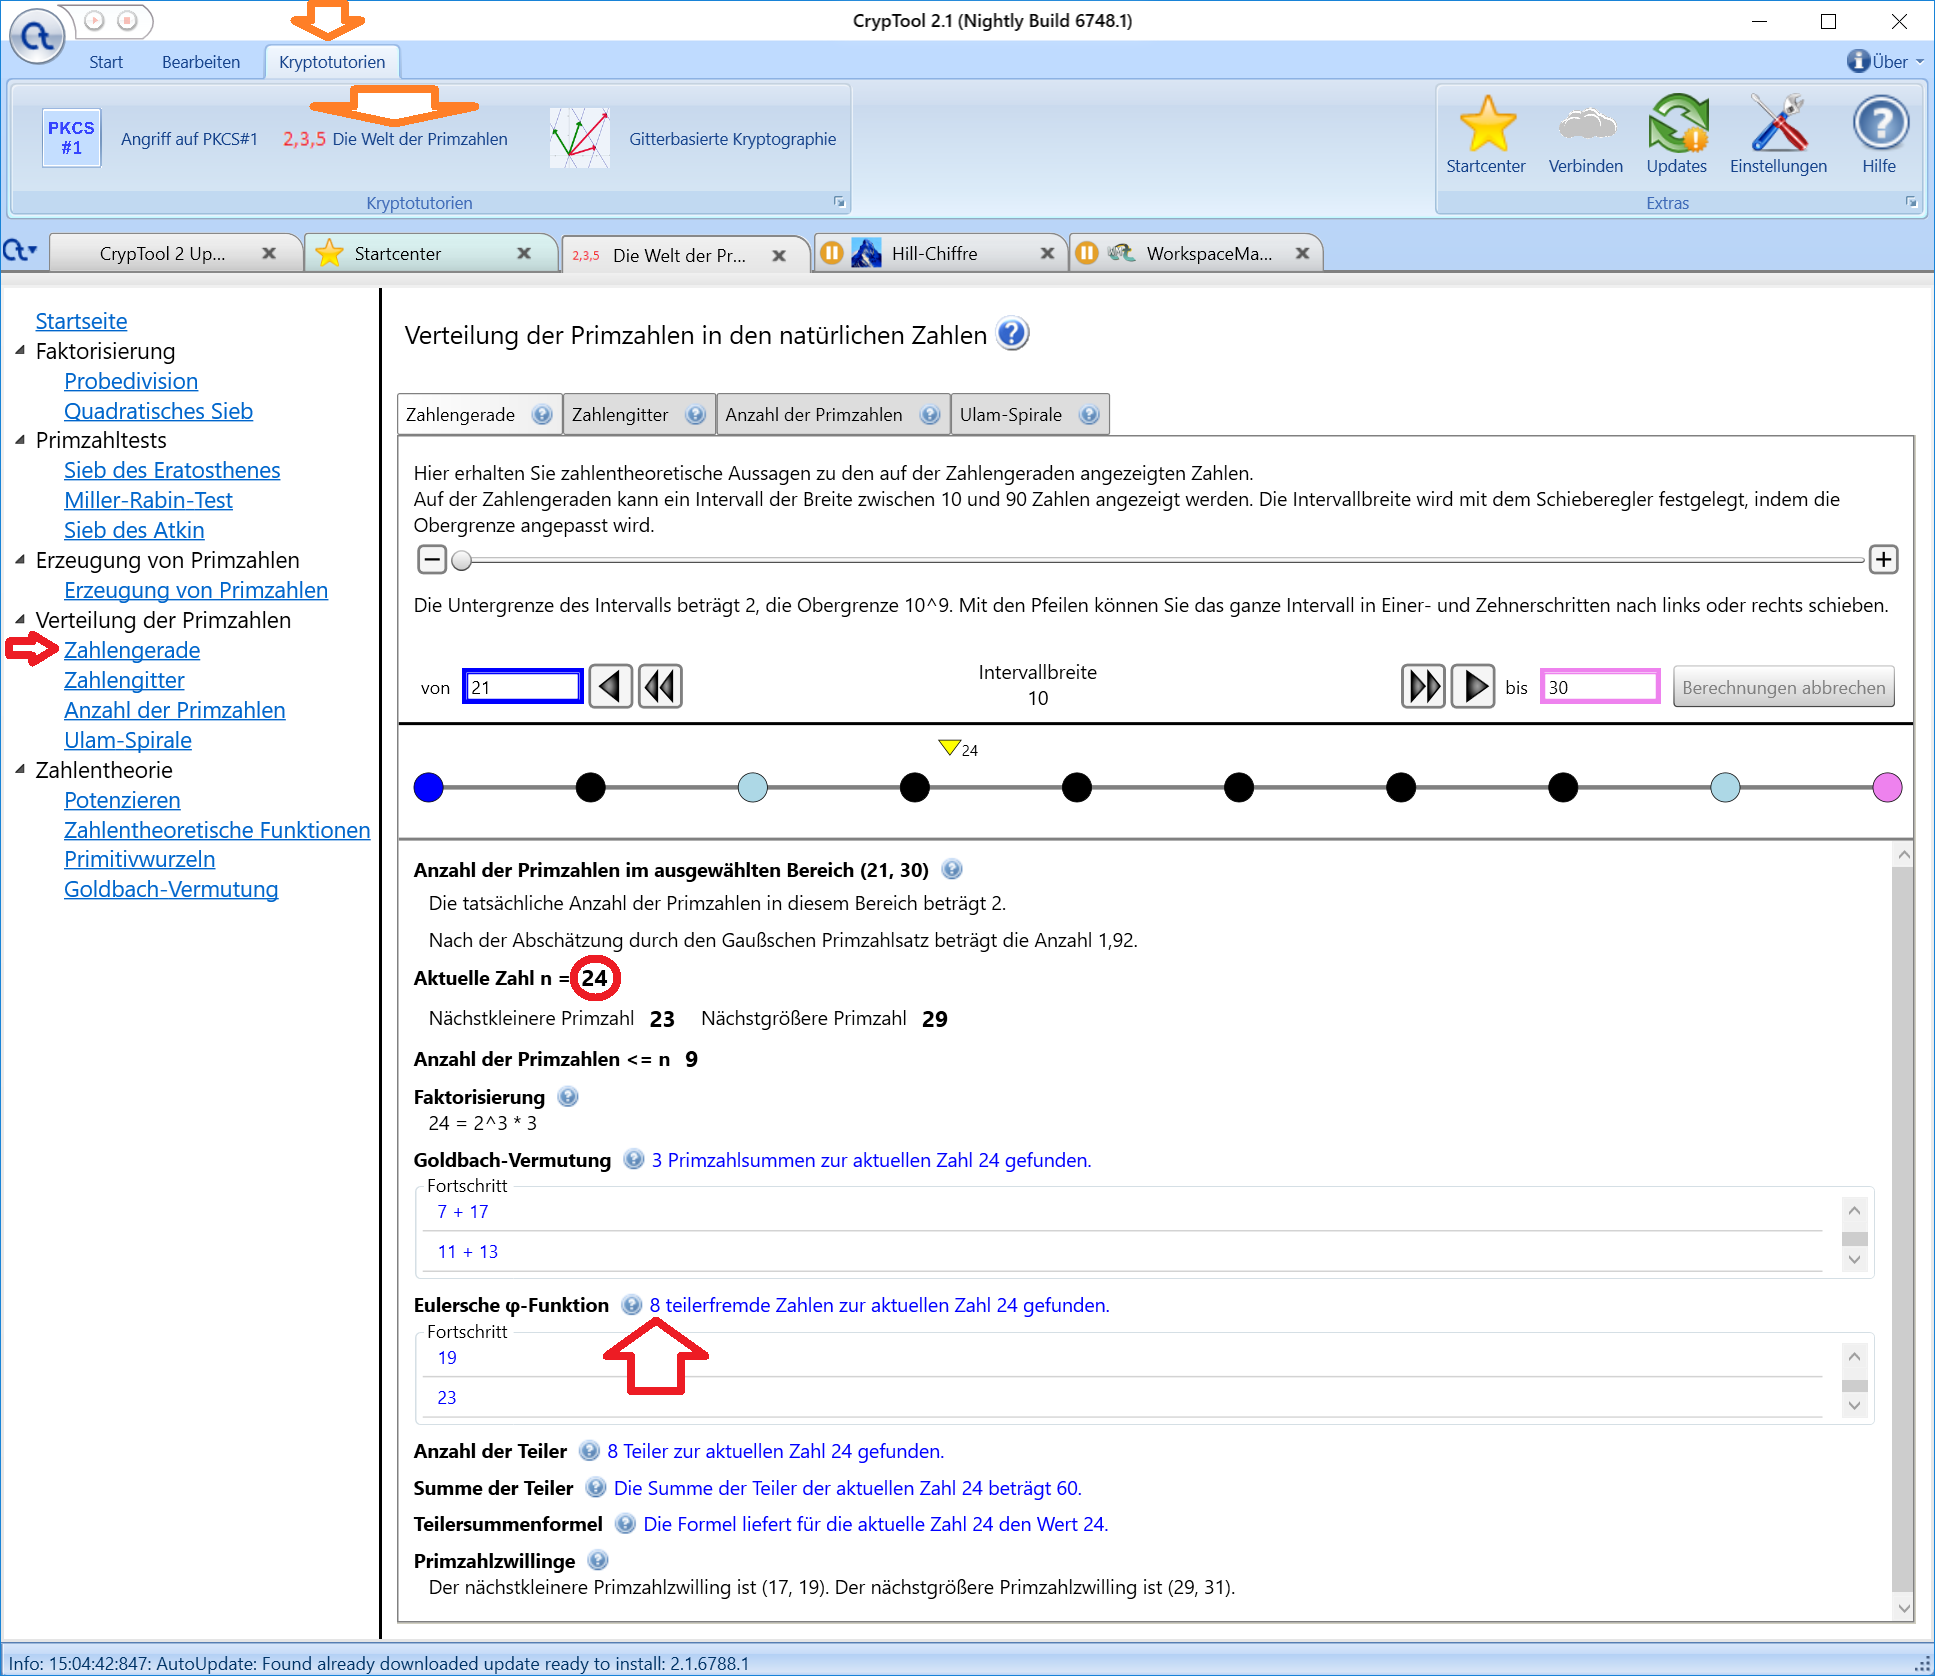
\includegraphics[scale=0.46]{figures/Euler-phi-of-24_in_CT2-WoP.png}
\caption[Zahlentheoretische Funktionen in CT2]
        {Zahlentheoretische Funktionen in CT2\protect\footnotemark}
\label{Euler-phi-of-24_in_CT2-WoP-figure}
\end{center}
\end{figure}
\footnotetext{%
   Grafik von CT2, Menü Kryptotutorien, Die Welt der Primzahlen,
   Verteilung der Primzahlen, Zahlengerade.\index{CT2}
}

\end{remark}
\newpage





% --------------------------------------------------------------------------
\subsection{Der Satz von Euler-Fermat}\index{Euler, Leonhard}\index{RSA}
\label{Label_KleinerSatzFermat-chap3}
Für den Beweis des RSA-Verfahrens brauchen wir den Satz von Fermat und
dessen Verallgemeinerung (Satz von Euler-Fermat) --
\hyperlink{KleinerSatzFermat-chap2}{vergleiche Kapitel~\ref{primality_tests}}.

\hypertarget{KleinerSatzFermat-chap3}{}
\index{Fermat!kleiner Satz}
\begin{satz}\label{thm-zth-fermat1}\textbf{Kleiner Satz von Fermat}\footnote{%
  Pierre de Fermat, französischer Mathematiker, 17.8.1601 -- 12.1.1665.
  \index{Fermat, Pierre}
}
\hypertarget{kleiner-Fermat}Sei $p$ eine Primzahl und $a$ eine beliebige ganze Zahl, dann gilt:
$$a^p \equiv a {\rm ~(mod~} p).$$
\end{satz}

Eine alternative Formulierung des kleinen Satzes von Fermat lautet:
Sei $p$ eine Primzahl und $a$ eine beliebige ganze Zahl, die
teilerfremd\index{Zahlen!teilerfremd (co-prime)} zu $p$ ist, dann gilt:
$$a^{p-1} \equiv 1 {\rm ~(mod~} p).$$
\begin{satz}{\label{thm-zth-fermateuler}}
\textbf{Satz von Euler-Fermat (Verallgemeinerung des kleines Satzes
von Fermat)}\hypertarget{Euler-Fermat}{}
Für alle Elemente $a$ aus der Gruppe $\mathbb{Z}_n^*$ gilt (d.h. $a$
und $n$ sind natürliche Zahlen, die teilerfremd zueinander sind):
$$  a^{\phi(n)} \equiv 1  {\rm ~(mod~} n).$$
\end{satz}
\index{Euler, Leonhard} \index{Fermat, Pierre}

Dieser Satz besagt, dass wenn man ein Gruppenelement (hier $a$) mit der
Ordnung der Gruppe (hier $\phi(n)$) potenziert,
ergibt sich immer das neutrale Element der Multiplikation (die Zahl 1).

Die 2. Formulierung des kleinen Satzes von Fermat ergibt sich direkt
aus dem Satz von Euler, wenn $n$ eine Primzahl ist.

Falls $n$ das Produkt zweier verschiedenen Primzahlen ist, kann man mit
dem Satz von Euler in bestimmten Fällen sehr schnell das Ergebnis einer
modularen Potenz berechnen.
Es gilt: $a^{(p-1)*(q-1)} \equiv 1 {\rm ~(mod~}pq)$.
\vskip +7 pt

\begin{example}{ Berechnung einer modularen Potenz:}
\vskip -4pt
\begin{itemize}
   \item Was ist $5^{2} {\rm ~(mod~}6)$ ?\\
         Mit $2 = 1 * 2$ und $6 = 2*3$, wobei $2$ und $3$ jeweils prim;
         $\phi(6) = 2$, da nur $1$ und $5$ zu $6$ teilerfremd
         \index{Zahlen!teilerfremd (co-prime)} sind, folgt
         $5^2 \equiv 5^{\phi(6)} \equiv 1 {\rm ~(mod~}6)$,
         ohne dass man die Potenz berechnen musste.
   \item Was ist $31^{792} {\rm ~(mod~}851)$ ?\\
         Mit $792 = 22 * 36$ und $23*37 = 851$, wobei $23$ und $37$ jeweils
         prim sind, folgt für $31 \in \mathbb{Z}_{851}^*$\\
         $31^{792} \equiv 31^{\phi(23*37)} \equiv 31^{\phi(851)} \equiv 1
         {\rm ~(mod~}851)$.
\end{itemize}
\end{example}

% --------------------------------------------------------------------------
\subsection{Bestimmung der multiplikativen Inversen}

Eine weitere interessante Anwendung ist ein Sonderfall der Bestimmung der
multiplikativen Inverse mit Hilfe des Satzes von Euler-Fermat
(multiplikative Inverse werden ansonsten mit dem \index{Euklidscher Algorithmus!erweiterter} erweiterten Euklid'schen
Algorithmus ermittelt).

\begin{example}{:}\\
Finde die multiplikative Inverse von $1579$ modulo $7351$.

Nach Euler-Fermat gilt: $a^{\phi(n)}= 1$ mod $n$ für alle $a$ aus $\mathbb{Z}_n^*$.
Teilt man beide Seiten durch $a$, ergibt sich: $a^{\phi(n) - 1} \equiv a^{-1}$ (mod $n$).
Für den Spezialfall, dass der Modul prim ist, gilt $\phi(n) = p - 1$.
Also gilt für die modulare Inverse $ a^{-1}$ von a:
$$a^{-1} \equiv a^{\phi(n) - 1} \equiv a^{(p-1)-1} \equiv a^{p-2} {\rm ~(mod~} p). $$
Für unser Beispiel bedeutet das:
\begin{itemize}
   \item[]  Da der Modul $7351$ prim ist, ist $p-2 = 7349$.\\
        $1579^{-1} \equiv 1579^{7349}$ (mod $p$).
\end{itemize}
Durch geschicktes Zerlegen des Exponenten kann man diese Potenz relativ einfach
berechnen\footnote{%
Siehe Kapitel~\ref{hohpot}, \glqq \nameref{hohpot}\grqq.
}:
\begin{itemize}
   \item[] $7349 = 4096 + 2048 + 1024 + 128 + 32 + 16 + 4 + 1$
   \item[] $1579^{-1} \equiv 4716$ (mod $7351$)
\end{itemize}
\end{example}

% --------------------------------------------------------------------------
%\subsection{Wie viele private RSA-Schlüssel d gibt es modulo 26}
%\subsection[Wie viele private RSA-Schlüssel d gibt es modulo 26]{Wie viele private RSA-Schlüssel $d$ gibt es modulo 26}
\subsection{Wie viele private RSA-Schlüssel \texorpdfstring{$d$}{d} gibt es modulo 26}
\label{L_nt_Num-of-d-mod-26}

Laut Satz~\ref{thm-zth-pot} werden die arithmetischen Operationen von modularen
Ausdrücken in den Exponenten modulo $\phi(n)$ und nicht modulo $n$
durchgeführt.\footnote{%
Für das folgende Beispiel wird der Modul wie beim RSA-Verfahren üblich mit
\glqq $n$\grqq~statt mit \glqq $m$\grqq~bezeichnet.}

Wenn man in $a^{e*d} \equiv a^1$ (mod $n$) die Inverse z.B. für den Faktor $e$
im Exponenten bestimmen will, muss man modulo $\phi(n)$ rechnen.

\begin{example}{:} (mit Bezug zum RSA-Algorithmus)\index{RSA}\\
Wenn man modulo $26$ rechnet, aus welcher Menge können $e$ und $d$ kommen?

Lösung: Es gilt $e*d \equiv 1$ (mod $\phi(26)$).
\begin{itemize}
   \item[] Die reduzierte Restmenge\index{Restmenge!reduziert}
$R' = \mathbb{Z}_{26}^* = \{ 1, 3, 5, 7, 9, 11, 15, 17, 19, 21, 23, 25 \}$ sind die
Elemente in $\mathbb{Z}_{26}, $ die eine multiplikative Inverse haben,
also teilerfremd
\index{Zahlen!teilerfremd (co-prime)}\index{Primzahl!relativ}\index{Zahlen!relativ prim}
zu $26$ sind (vgl. \ref{def-zth-znmult}).
   \item[] Die reduzierte Restmenge $R''$ enthält nur die Elemente aus
           $R'$, die teilerfremd zu $\phi(26) = 12$ sind:
           $R'' = \{ 1, 5, 7, 11 \}$.
   \item[] Für jedes $e$ aus $R''$ gibt es ein $d$ aus $R''$, so dass
           $a \equiv (a^e)^d{\rm ~(mod~}n)$.
\end{itemize}
Somit gibt es also zu jedem $e$ in $R''$ genau ein (nicht unbedingt von
$e$ verschiedenes) Element, so dass gilt: $e*d \equiv 1$ (mod $\phi(26)$).

Der allgemeine Fall, wo $n$ beliebige natürliche Zahlen annehmen kann (in
dem Beispiel hier galt ja immer $n = 26$), wird in Kapitel
\ref{l:NumberTheory_Sage_Number-of-RSA-keys} behandelt. Dort ist auch ein
SageMath-Programm, das die Anzahl aller $d$ liefert. Für alle $e$, die
teilerfremd\index{Zahlen!teilerfremd (co-prime)} zu $\phi(n)$ sind, kann man
das $d$ nach dem Satz von Euler-Fermat folgendermaßen berechnen:
\begin{eqnarray*}
 d & \equiv & e^{-1}      {\rm ~(mod~} \phi(n)) \nonumber\\
   & \equiv & e^{\phi(\phi(n))-1}  {\rm ~(mod~} \phi(n)), \quad  {\rm denn~}  a^{\phi(n)} \equiv 1 {\rm ~(mod~} n)
      \quad {\rm ~entspricht~~} a^{\phi(n)-1} \equiv a^{-1} {\rm ~(mod~} n). \nonumber
\end{eqnarray*}
\end{example}

Besteht die Zahl $n$ aus zwei verschiedenen Primfaktoren (und sind noch ein
paar weitere Kriterien erfüllt), so sind die Faktorisierung\index{Faktorisierung!Faktorisierungsproblem} von $n$ und das Finden von $\phi(n)$ ähnlich schwierig\footnote{%
Für $n=pq$  mit $p\neq q$ gilt $ \phi(n) = (p-1)*(q-1)
= n -(p+q)+1.$ Ferner sind die Zahlen $p$ und $q$ Lösungen der quadratischen Gleichung
$x^2-(p+q)x+pq=0. $\\
Sind nur
$n$ und $\phi(n)$ bekannt, so gilt $pq=n$ und $p+q= n +1 -\phi(n).$  Man erhält somit die Faktoren $p$ und $q$ von $n$, indem man die folgende quadratische Gleichung löst:
$$ x^2 +(\phi(n)-n-1)x +n=0 $$\vspace{-\baselineskip}
}
(vergleiche Forderung 3 in \hyperlink{Chapter_ElementaryNT_10_1}
{Kapitel~\ref{Label_Chapter_ElementaryNT_10_1}}).



% ++++++++++++++++++++++++++++++++++++++++++++++++++++++++++++++++++++++++++
\hypertarget{Chapter_ElementaryNT_9}{}
\section[Multiplikative Ordnung und Primitivwurzel]
        {Multiplikative Ordnung und Primitivwurzel\footnotemark}
\footnotetext{%
    \index{ZT, Lernprogramm Zahlentheorie}%
    \index{Lernprogramm ZT}%
    \index{Primitivwurzel}%
    Mit dem Lernprogramm \textbf{ZT} können Sie einige der hier besprochenen
    Verfahren vertiefen (siehe Lern-Kapitel 2.2, Seiten 10-14/40 und 24-40/40).\\
    ZT können Sie in CT1\index{CT1} über das Menü
    \textbf{Einzelverfahren \textbackslash{} Zahlentheorie
    interaktiv \textbackslash{} Lernprogramm für Zahlentheorie} aufrufen.
    Siehe Anhang~\ref{s:appendix-Learn-NT}.\\
    Siehe auch die SageMath-Beispiele in \ref{nt:AppArith3a1}.
}
\label{MultOrdPrimitveRoot}

Die Multiplikative Ordnung (order) und die Primitivwurzel (primitive root)
sind zwei nützliche Konstrukte (Konzepte) der elementaren Zahlentheorie.

Mathematiker stellen sich die Frage, unter welchen Bedingungen ergibt
die wiederholte Anwendung einer Operation das neutrale Element
(vergleiche \hyperlink{patternsandstructures}{Muster und Strukturen},
Kapitel~\ref{patternsandstructures}\index{Struktur}).

Für die $i$-fach aufeinander folgende modulare Multiplikation einer
Zahl $a$ für \mbox{$i=1, \dots, m-1$} ergibt sich als Produkt das neutrale
Element der Multiplikation nur dann, wenn $a$ und $m$
teilerfremd\index{Zahlen!teilerfremd (co-prime)} sind.

\begin{definition}\label{def-zth-ordn}
Die \textbf{multiplikative Ordnung} \index{Ordnung!multiplikativ}
$ord_m(a)$ einer ganzen Zahl $a {\rm ~(mod~} m)$ (wobei $a$ und $m$
teilerfremd sind) ist die kleinste ganze Zahl $i$, für die gilt:
 $a^i \equiv 1 {\rm ~(mod~} m)$.
\end{definition}

Die folgende Tabelle~\ref{expmod11} zeigt, dass in einer multiplikativen Gruppe
(hier $\mathbb{Z}_{11}^*$) nicht notwen"-dig alle Zahlen die gleiche Ordnung
haben: Die Ordnungen sind $1, 2, 5$ und $10$. Es gilt:
\begin{enumerate}
  \item Die Ordnungen sind alle Teiler von 10.
  \item Die Zahlen $a = 2, 6, 7$ und $8$ haben die Ordnung $10$.
        Man sagt diese Zahlen haben in $\mathbb{Z}_{11}^*$
        \textbf{maximale Ordnung}\index{Ordnung!maximal}.
\end{enumerate}

\newpage
\begin{example}{ 1:}\\
Die folgende Tabelle~\ref{expmod11}\footnote{%
  Das SageMath-Beispiel~\ref{nt_Sage-code_MultOrder_expmod11} enthält den
  Quelltext zur Berechnung der Tabelle~\ref{expmod11}.
  Siehe Kapitel~\ref{nt:AppArith3a1} \glqq \nameref{nt:AppArith3a1}\grqq.}
zeigt die Werte $a^i{\rm ~mod~}11$ für die Exponenten $i = 1, 2, \cdots, 10$
und für die Basen $a = 1, 2, \cdots, 10$, sowie den sich für jedes a daraus
ergebenden Wert $ord_{11}(a)$.
\end{example}\\

\begin{table}[ht]
\begin{center} \label{SrcArith3a}
\begin{tabular}{|l||c|c|c|c|c|c|c|c|c|c|c|c|c|c|}
\hline
              & i=1 & i=2 & i=3 & i=4 & i=5 & i=6 & i=7 & i=8 & i=9 & i=10  & $ord_{11}(a)$\\
\hline
\hline
a=1           & \textbf{1}  & 1    & 1  & 1    & 1    & 1    & 1  & 1    & 1  & 1     & 1\\
\hline
a=2           & 2  & 4    & 8  & 5   & 10    & 9    & 7  & 3    & 6  & \textbf{1}    & 10\\
\hline
a=3           & 3  & 9    & 5  & 4 & \textbf{1} & 3    & 9  & 5    & 4  & 1     & 5\\
\hline
a=4           & 4  & 5    & 9  & 3 & \textbf{1} & 4    & 5  & 9    & 3  & 1    & 5\\
\hline
a=5           & 5  & 3    & 4  & 9 & \textbf{1} & 5    & 3  & 4    & 9  & 1    & 5\\
\hline
a=6           & 6  & 3    & 7  & 9   & 10    & 5    & 8  & 4    & 2  & \textbf{1}    & 10\\
\hline
a=7           & 7  & 5    & 2  & 3   & 10    & 4    & 6  & 9    & 8  & \textbf{1}    & 10\\
\hline
a=8           & 8  & 9    & 6  & 4   & 10    & 3    & 2  & 5    & 7  & \textbf{1}    & 10\\
\hline
a=9           & 9  & 4    & 3  & 5 & \textbf{1} & 9    & 4  & 3    & 5  & 1    & 5\\
\hline
a=10         & 10  & \textbf{1}   & 10  & 1   & 10    & 1   & 10  & 1   & 10  & 1    & 2\\
\hline
\end{tabular}
\end{center}
\caption{Werte von $a^i{\rm ~mod~}11, 1\leq a,i<11$ und zugehörige Ordnung von $a$ modulo $11$}
\label{expmod11}
\end{table}

\noindent Aus der Tabelle~\ref{expmod11} kann man ersehen, dass z.B. die
Ordnung von $3$ modulo $11$ den Wert $5$ hat.\\


\begin{definition}\label{def-zth-primitiveroot}
Sind $a$ und $m$ teilerfremd\index{Zahlen!teilerfremd (co-prime)} und
gilt $ord_m(a) = \phi(m)$, (d.h. $a$ hat maximale Ordnung), dann nennt man
$a$ eine \textbf{Primitivwurzel} \index{Primitivwurzel} von $m$.\footnote{%
  In Kapitel~\ref{nt:AppArith3a2}, \glqq \nameref{nt:AppArith3a2}\grqq~finden Sie
  SageMath-Programme zur Berechnung von Primitivwurzeln.%%\label{primitive-roots-with-sage}
}
\end{definition}

Nicht zu jedem Modul $m$ gibt es eine Zahl $a$, die eine
Primitivwurzel\index{Primitivwurzel} ist. %%% Gibt es m, die keine Primitivwurzel haben?
In der Tabelle~\ref{expmod11} sind nur $a = 2, 6, 7$ und $8$ bezüglich mod
$11$ eine Primitivwurzel\index{Primitivwurzel} ($ord_m(a) = \phi(11) = 10$).

Mit Hilfe der Primitivwurzel\index{Primitivwurzel} kann man die Bedingungen
klar herausarbeiten, wann Potenzen modulo $m$ {\em eindeutig invertierbar}
\index{invertierbar} sind und die Berechnung in den Exponenten handhabbar
ist.\footnote{%
  Eine gute Übersicht zu Primitivwurzeln findet sich auch in Wikipedia:
  \url{https://de.wikipedia.org/wiki/Primitivwurzel} und vor allem
  \url{https://en.wikipedia.org/wiki/Primitive_root_modulo_n}.
}

Die folgenden beiden Tabellen \ref{expmod45} und \ref{expmod46} zeigen
multiplikative Ordnung und Primitivwurzel\index{Primitivwurzel} modulo
$45$ und modulo $46$.

\newpage
\begin{example}{ 2:}\\
Die folgende Tabelle~\ref{expmod45}\footnote{%
  Das SageMath-Beispiel~\ref{nt_Sage-code_MultOrder_expmod45} enthält den
  Quelltext zur Berechnung der Tabelle~\ref{expmod45}.
  Siehe Kapitel~\ref{nt:AppArith3b}, \glqq \nameref{nt:AppArith3b}\grqq.}
zeigt die Werte $a^i{\rm ~mod~}45$ für die Exponenten $i = 1, 2, \cdots, 12$
und für die Basen $a = 1, 2, \cdots, 12$ sowie den sich für jedes $a$ daraus
ergebenden Wert $ord_{45}(a)$.
\end{example}

\begin{table}[ht]
\begin{center} \label{SrcArith3b}
\begin{tabular}{|l||c|c|c|c|c|c|c|c|c|c|c|c|c|c|c|c|c|c|c|c|c|c|c|c|c|}
\hline
 $a\setminus i$ & 1            & 2            & 3 & 4 & 5 & 6 & 7 & 8 & 9 & 10 & 11 & 12     & $ord_{45}(a)$       & $\phi(45)$\\
\hline
\hline
1             & 1              & 1   & 1   & 1   & 1   & 1   & 1   & 1   & 1    & 1    & 1    & 1 & 1              & 24\\
\hline
2             & 2              & 4   & 8  & 16  & 32  & 19  & 38  & 31  & 17   & 34   & 23    & 1 & 12             & 24\\
\hline
3             & 3              & 9  & 27  & 36  & 18   & 9  & 27  & 36  & 18    & 9   & 27   & 36  & ---            & 24\\
\hline
4             & 4             & 16  & 19  & 31  & 34   & 1   & 4  & 16  & 19   & 31   & 34    & 1  & 6              & 24\\
\hline
5             & 5             & 25  & 35  & 40  & 20  & 10   & 5  & 25  & 35   & 40   & 20   & 10  & ---            & 24\\
\hline
6             & 6             & 36  & 36  & 36  & 36  & 36  & 36  & 36  & 36   & 36   & 36   & 36  & ---            & 24\\
\hline
7             & 7              & 4  & 28  & 16  & 22  & 19  & 43  & 31  & 37   & 34   & 13    & 1  & 12             & 24\\
\hline
8             & 8             & 19  & 17   & 1   & 8  & 19  & 17   & 1   & 8   & 19   & 17    & 1  & 4              & 24\\
\hline
9             & 9             & 36   & 9  & 36   & 9  & 36   & 9  & 36   & 9   & 36    & 9   & 36  & ---            & 24\\
\hline
10           & 10             & 10  & 10  & 10  & 10  & 10  & 10  & 10  & 10   & 10   & 10   & 10  & ---            & 24\\
\hline
11           & 11             & 31  & 26  & 16  & 41   & 1  & 11  & 31  & 26   & 16   & 41    & 1  & 6              & 24\\
\hline
12           & 12              & 9  & 18  & 36  & 27   & 9  & 18  & 36  & 27    & 9   & 18   & 36  & ---            & 24\\
\hline
\end{tabular}
\end{center}
\caption{Werte von $a^i{\rm ~mod~}45, 1\leq a,i<13$ und zugehörige Ordnung von $a$ modulo $45$}
\label{expmod45}
\end{table}

\vskip +10 pt
\noindent $\phi(45)$ berechnet sich nach Satz~\ref{J_of_n}: $\phi(45) = \phi(3^2*5) = [3^1*2] * [1*4] = 24$.

\noindent Da $45$ keine Primzahl ist, gibt es nicht für alle Werte von $a$
eine \glqq Multiplikative Ordnung\grqq~(für alle nicht zu $45$
teilerfremden\index{Zahlen!teilerfremd (co-prime)} Zahlen:
$3, 5, 6, 9, 10, 12, \cdots,$ da $45 = 3^2*5$).



\vspace{\baselineskip}
\vspace{\baselineskip}
\begin{example}{ 3:}\\
Hat $7$ eine Primitivwurzel\index{Primitivwurzel} modulo $45$?

\noindent Die notwendige, aber nicht hinreichende Voraussetzung/Bedingung
ggT$(7,45)=1$ ist erfüllt.
Aus der Tabelle~\ref{expmod45} kann man ersehen, dass die
Zahl $a=7$ keine Primitivwurzel\index{Primitivwurzel} von $45$ ist,
denn $ord_{45}(7) = 12 \not= 24 = \phi(45)$.%\vskip + 1em
\end{example}



\newpage
\begin{example}{ 4:}\\
Die folgende Tabelle~\ref{expmod46}\footnote{%
  Das SageMath-Beispiel~\ref{nt_Sage-code_MultOrder_expmod46} enthält den
  Quelltext zur Berechnung der Tabelle~\ref{expmod46}.
  Siehe Kapitel~\ref{nt:AppArith3c}, \glqq \nameref{nt:AppArith3c}\grqq.}
beantwortet die Frage, ob die Zahl $a=7$ eine Primitivwurzel\index{Primitivwurzel} von $46$ ist.

\noindent Die notwendige, aber nicht hinreichende Voraussetzung/Bedingung
ggT$(7,46)=1$ ist erfüllt.\\
$\phi(46)$ berechnet sich nach Satz~\ref{J_of_pq}: $\phi(46) = \phi(2*23) = 1*22 = 22$.
Die Zahl $7$ ist eine Primitivwurzel\index{Primitivwurzel} von $46$,
denn $ord_{46}(7) = 22 = \phi(46)$.
\end{example}

\begin{table}[ht]
\label{SrcArith3c}
{\textmd \small
\begin{center}
%\vspace{-5ex}  %Dieses vspace bewirkte, dass die Überschrift in der Tab. stand.
\vspace{-2ex}  % Rein, damit Kap. 4.10 oben auf der ff. Seite beginnt.
\begin{tabular}{|p{16 pt}||@{\:}r@{\:}|@{\:}r@{\:}|@{\:}r@{\:}|@{\:}r@{\:}|@{\:}r@{\:}|@{\:}r@{\:}|@{\:}r@{\:}|@{\:}r@{\:}|@{\:}r@{\:}|@{\:}r@{\:}|@{\:}r@{\:}|@{\:}r@{\:}|@{\:}r@{\:}|@{\:}r@{\:}|@{\:}r@{\:}|@{\:}r@{\:}|@{\:}r@{\:}|@{\:}r@{\:}|@{\:}r@{\:}|@{\:}r@{\:}|@{\:}r@{\:}|@{\:}r@{\:}|@{\:}r@{\:}|c|}
\hline
$a \setminus i$   & 1 & 2 & 3 & 4 & 5 & 6 & 7 & 8 & 9 & 10 & 11 & 12 & 13 & 14 & 15 & 16 & 17 & 18 & 19 & 20 & 21 & 22 & 23 & ord\\
\hline
\hline
1    & 1  & 1  & 1  & 1  & 1  & 1  & 1  & 1  & 1  & 1  & 1  & 1  & 1  & 1  & 1  & 1  & 1  & 1  & 1  & 1  & 1  & 1  & 1 & 1\\
\hline
2 & 2  & 4  & 8 & 16 & 32 & 18 & 36 & 26  & 6 & 12 & 24  & 2  & 4  & 8 & 16 & 32 & 18 & 36 & 26  & 6 & 12 & 24  & 2 & --\\
\hline
3 & 3  & 9 & 27 & 35 & 13 & 39 & 25 & 29 & 41 & 31  & 1  & 3  & 9 & 27 & 35 & 13 & 39 & 25 & 29 & 41 & 31  & 1  & 3 & 11\\
\hline
4  & 4 & 16 & 18 & 26 & 12  & 2  & 8 & 32 & 36  & 6 & 24  & 4 & 16 & 18 & 26 & 12  & 2  & 8 & 32 & 36  & 6 & 24  & 4 & --\\
\hline
5 & 5 & 25 & 33 & 27 & 43 & 31 & 17 & 39 & 11  & 9 & 45 & 41 & 21 & 13 & 19  & 3 & 15 & 29  & 7 & 35 & 37  & 1  & 5 & 22\\
\hline
6 & 6 & 36 & 32  & 8  & 2 & 12 & 26 & 18 & 16  & 4 & 24  & 6 & 36 & 32  & 8  & 2 & 12 & 26 & 18 & 16  & 4 & 24  & 6 & --\\
\hline
7 & 7  & 3 & 21  & 9 & 17 & 27  & 5 & 35 & 15 & 13 & 45 & 39 & 43 & 25 & 37 & 29 & 19 & 41 & 11 & 31 & 33  & \textbf{1}  & 7 & 22\\
\hline
8 & 8 & 18  & 6  & 2 & 16 & 36 & 12  & 4 & 32 & 26 & 24  & 8 & 18  & 6  & 2 & 16 & 36 & 12  & 4 & 32 & 26 & 24  & 8 & --\\
\hline
9 & 9 & 35 & 39 & 29 & 31  & 3 & 27 & 13 & 25 & 41  & 1  & 9 & 35 & 39 & 29 & 31  & 3 & 27 & 13 & 25 & 41  & 1  & 9 & 11\\
\hline
10 & 10  & 8 & 34 & 18 & 42  & 6 & 14  & 2 & 20 & 16 & 22 & 36 & 38 & 12 & 28  & 4 & 40 & 32 & 44 & 26 & 30 & 24 & 10 & --\\
\hline
11 & 11 & 29 & 43 & 13  & 5  & 9  & 7 & 31 & 19 & 25 & 45 & 35 & 17  & 3 & 33 & 41 & 37 & 39 & 15 & 27 & 21  & 1 & 11 & 22\\
\hline
12 & 12  & 6 & 26 & 36 & 18 & 32 & 16  & 8  & 4  & 2 & 24 & 12  & 6 & 26 & 36 & 18 & 32 & 16  & 8  & 4  & 2 & 24 & 12 & --\\
\hline
13 & 13 & 31 & 35 & 41 & 27 & 29  & 9 & 25  & 3 & 39  & 1 & 13 & 31 & 35 & 41 & 27 & 29  & 9 & 25  & 3 & 39  & 1 & 13 & 11\\
\hline
14 & 14 & 12 & 30  & 6 & 38 & 26 & 42 & 36 & 44 & 18 & 22 & 32 & 34 & 16 & 40  & 8 & 20  & 4 & 10  & 2 & 28 & 24 & 14 & --\\
\hline
15 & 15 & 41 & 17 & 25  & 7 & 13 & 11 & 27 & 37  & 3 & 45 & 31  & 5 & 29 & 21 & 39 & 33 & 35 & 19  & 9 & 43  & 1 & 15 & 22\\
\hline
16 & 16 & 26  & 2 & 32  & 6  & 4 & 18 & 12  & 8 & 36 & 24 & 16 & 26  & 2 & 32  & 6  & 4 & 18 & 12  & 8 & 36 & 24 & 16 & --\\
\hline
17 & 17 & 13 & 37 & 31 & 21 & 35 & 43 & 41  & 7 & 27 & 45 & 29 & 33  & 9 & 15 & 25 & 11  & 3  & 5 & 39 & 19  & 1 & 17 & 22\\
\hline
18 & 18  & 2 & 36  & 4 & 26  & 8  & 6 & 16 & 12 & 32 & 24 & 18  & 2 & 36  & 4 & 26  & 8  & 6 & 16 & 12 & 32 & 24 & 18 & --\\
\hline
19  & 19 & 39  & 5  & 3 & 11 & 25 & 15  & 9 & 33 & 29 & 45 & 27  & 7 & 41 & 43 & 35 & 21 & 31 & 37 & 13 & 17  & 1 & 19 & 22\\
\hline
20  & 20 & 32 & 42 & 12 & 10 & 16 & 44  & 6 & 28  & 8 & 22 & 26 & 14  & 4 & 34 & 36 & 30  & 2 & 40 & 18 & 38 & 24 & 20 & --\\
\hline
21 & 21 & 27 & 15 & 39 & 37 & 41 & 33  & 3 & 17 & 35 & 45 & 25 & 19 & 31  & 7  & 9  & 5 & 13 & 43 & 29 & 11  & 1 & 21 & 22\\
\hline
22 & 22 & 24 & 22 & 24 & 22 & 24 & 22 & 24 & 22 & 24 & 22 & 24 & 22 & 24 & 22 & 24 & 22 & 24 & 22 & 24 & 22 & 24 & 22 & --\\
\hline
23 & 23 & 23 & 23 & 23 & 23 & 23 & 23 & 23 & 23 & 23 & 23 & 23 & 23 & 23 & 23 & 23 & 23 & 23 & 23 & 23 & 23 & 23 & 23 & --\\
\hline
\end{tabular}
\end{center}
}
\caption{Werte von $a^i{\rm ~mod~}46, 1\leq a,i<24$ und zugehörige Ordnung von $a$ modulo $46$}
\label{expmod46}
\end{table}


\vskip +10 pt
\begin{satz}\label{thm-zth-ordp}
Für einen Modul $n$ und eine Zahl $a$,
teilerfremd\index{Zahlen!teilerfremd (co-prime)} zu $n$ gilt:\\
Die Menge $\{ a^i\; (\mbox{mod }n) |\; i = 1,\dots,\phi(n)\}$ ist gleich
der multiplikativen Gruppe $Z_n^*$ genau dann, wenn  $ord_n(a) = \phi(n)$.\footnote{%
    Für Primmoduli $p$ haben alle $a$ mit $0 < a < p$ die Ordnung $\phi(p) = p
    - 1$.  Vergleiche dazu Tabelle~\ref{expmod45}. In diesem Fall nimmt $a^i (\mbox{mod
    }n)$ alle Werte $1,\dots,p-1$ an. Dieses Ausschöpfen des
    Wertebereiches\index{Wertebereich} ist eine wichtige kryptographische
    Eigenschaft (vergleiche Satz~\ref{thm-zth-exhperm}). Hiermit wird eine
    Permutation\index{Permutation} $\pi(p-1)$ festgelegt.
}${}^,$\footnote{%
Tabelle~\ref{expmod46} zeigt, dass bei zusammengesetzten Moduli $n$ nicht alle $a$ die
maximale Ordnung $\phi(n)$ haben. In diesem Beispiel haben nur $5,7,11,15,17,19
\mbox{ und } 21$
die Ordnung 22.
}
\end{satz}
\noindent Die multiplikative Gruppe $Z_n^*$ nimmt nur dann alle Werte von $1$ bis $n-1$
an, wenn n prim ist (vgl. Definition \ref{def-zth-znmult}).




\newpage
\begin{example}{ 5: Zykluslängen}

\noindent Die folgenden Tabellen~\ref{expmod14} und~\ref{expmod22}\footnote{%
  In Kapitel~\ref{nt:AppArith3d}, \glqq \nameref{nt:AppArith3d}\grqq~
  finden Sie den Quelltext zur Berechnung der Tabellen~\ref{expmod14} und~\ref{expmod22}
  mit SageMath.
} dienen als Beispiele, um Zykluslängen\index{Zykluslänge} zu betrachten -- ein
Thema, das über die multiplikative Ordnung hinausführt.

\noindent Als Zyklus bezeichnet man hier eine Folge von Zahlen $a^i{\rm ~mod~}n$
mit $1\leq i<n$ für ein festes $a$, wobei sich die Folge wiederholt. Hier kommt
innerhalb eines Zyklus jede Zahl nur einmal vor (aufgrund der Erzeugung als
modulare Potenz). Die Zyklen hier müssen die $1$ nicht enthalten -- es sei
denn, dieser Zyklus gehört zu einer multiplikativen Ordnung $\ge 1$
(diese haben die $1$ immer am Ende des Zyklus und an der Stelle
$a^{n-1} ~mod~n$).\\
\noindent Im Folgenden bezeichnet $l$ die Zykluslänge.

\noindent Die maximale Zykluslänge $l_{max}$ ist $\phi(n)$.

\noindent Für die folgenden Tabellen~\ref{expmod14} und~\ref{expmod22} gilt
(nach Satz~\ref{J_of_n}):\\
\indent  - $\phi(14) = \phi(2*7) = 1*6 = 6$.\\
\indent  - $\phi(22) = \phi(2*11) = 1*10 = 10$.

\noindent a) Falls die multiplikative Ordnung für $a$ existiert, gilt (egal
ob $a$ prim ist): $ord_{n}(a) = l$.
\indent Beispiele: Die maximale Länge $l_{max}$\footnote{%
            Wir kennen keine Formel, für welche a die maximale Länge erreicht wird.}
wird beispielsweise erreicht für:\\
\indent  - $a=3$ mit $l_{max} = ord_{14}(a) = 6$ in Tabelle~\ref{expmod14}, oder\\
\indent  - $a=10$ mit $l_{max} = ord_{22}(a) = 10$ in Tabelle~\ref{expmod22}.

\noindent b) Auch wenn für $a$ keine multiplikative Ordnung existiert, kann
die Zykluslänge maximal sein.\footnote{%
         Die Folgen hier werden gebildet per $a^i{\rm ~mod~}n$ mit $1\leq i<n$,
         und enthalten für zusammengesetzte $n$ nie alle Zahlen $1, ..., n-1$.\\
         Dies ist nicht zu verwechseln mit RSA, wo die \glqq Folge\grqq~anders
         gebildet wird,  $m^e{\rm ~mod~}n$ mit $0\leq m<n$, und diese Folge
         dann alle Zahlen $0, ..., n-1$ durchläuft (Permutation).
}\\
\indent Beispiele:\\
\indent  - In Tabelle~\ref{expmod14} ist $l_{max}=\phi(14)=6$ für $a=10, 12$.\\
\indent  - In Tabelle~\ref{expmod22} ist $l_{max}=\phi(22)=10$ für $a=2, 6, 8, 18$.

\end{example}



\begin{table}[ht]
\begin{center}
\begin{tabular}{|l||c|c|c|c|c|c|c|c|c|c|c|c|c||c|c|c|}
\hline
$a \setminus i$ & 1 & 2 & 3 & 4 & 5 & 6 & 7 & 8 & 9 & 10 & 11 & 12 & 13 & $ord_{14}(a)$       & $\phi(14)$ & $l$\\
\hline
\hline
1 & 1 & 1 & 1 & 1 & 1 & 1 & 1 & 1 & 1 & 1 & 1 & 1 & 1 & 1 & 6 & 1\\
\hline
2 & 2 & 4 & 8 & 2 & 4 & 8 & 2 & 4 & 8 & 2 & 4 & 8 & 2 & 0 & 6 & 3\\
\hline
3 & 3 & 9 & 13 & 11 & 5 & 1 & 3 & 9 & 13 & 11 & 5 & 1 & 3 & 6 & 6 & 6\\
\hline
4 & 4 & 2 & 8 & 4 & 2 & 8 & 4 & 2 & 8 & 4 & 2 & 8 & 4 & 0 & 6 & 3\\
\hline
5 & 5 & 11 & 13 & 9 & 3 & 1 & 5 & 11 & 13 & 9 & 3 & 1 & 5 & 6 & 6 & 6\\
\hline
6 & 6 & 8 & 6 & 8 & 6 & 8 & 6 & 8 & 6 & 8 & 6 & 8 & 6 & 0 & 6 & 2\\
\hline
7 & 7 & 7 & 7 & 7 & 7 & 7 & 7 & 7 & 7 & 7 & 7 & 7 & 7 & 0 & 6 & 1\\
\hline
8 & 8 & 8 & 8 & 8 & 8 & 8 & 8 & 8 & 8 & 8 & 8 & 8 & 8 & 0 & 6 & 1\\
\hline
9 & 9 & 11 & 1 & 9 & 11 & 1 & 9 & 11 & 1 & 9 & 11 & 1 & 9 & 3 & 6 & 3\\
\hline
10 & 10 & 2 & 6 & 4 & 12 & 8 & 10 & 2 & 6 & 4 & 12 & 8 & 10 & 0 & 6 & 6\\
\hline
11 & 11 & 9 & 1 & 11 & 9 & 1 & 11 & 9 & 1 & 11 & 9 & 1 & 11 & 3 & 6 & 3\\
\hline
12 & 12 & 4 & 6 & 2 & 10 & 8 & 12 & 4 & 6 & 2 & 10 & 8 & 12 & 0 & 6 & 6\\
\hline
13 & 13 & 1 & 13 & 1 & 13 & 1 & 13 & 1 & 13 & 1 & 13 & 1 & 13 & 2 & 6 & 2\\
\hline
14 & 0 & 0 & 0 & 0 & 0 & 0 & 0 & 0 & 0 & 0 & 0 & 0 & 0 & 0 & 6 & 1\\
% Ab hier wiederholen sich die Zeilen --> statt Doppellinie:
% The arydshln package offers you the \hdashline and \cdashline commands which
% are the dashed counterparts of \hline and \cline, respectively.
\hdashline
\hdashline
% \hdashline[1pt/5pt]
% \hline
% \hline
15 & 1 & 1 & 1 & 1 & 1 & 1 & 1 & 1 & 1 & 1 & 1 & 1 & 1 & 1 & 6 & 1\\
\hline
16 & 2 & 4 & 8 & 2 & 4 & 8 & 2 & 4 & 8 & 2 & 4 & 8 & 2 & 0 & 6 & 3\\
\hline
\end{tabular}
\end{center}
\caption{Werte von $a^i{\rm ~mod~}14, 1\leq a<17, i<14$}
\label{expmod14}
\end{table}


\newpage
\begin{table}[ht]
\begin{center}
% \begin{tabular}{|l||c|c|c|c|c|c|c|c|c|c|c|c|c|c|c|c|c|c|c|c|c||c|c|}
% Tabular modifiziert, damit enger und nicht über Seitenrand rausgeht
\begin{tabular}{|p{16 pt}||@{\:}r@{\:}|@{\:}r@{\:}|@{\:}r@{\:}|@{\:}r@{\:}|@{\:}r@{\:}|@{\:}r@{\:}|@{\:}r@{\:}|@{\:}r@{\:}|@{\:}r@{\:}|@{\:}r@{\:}|@{\:}r@{\:}|@{\:}r@{\:}|@{\:}r@{\:}|@{\:}r@{\:}|@{\:}r@{\:}|@{\:}r@{\:}|@{\:}r@{\:}|@{\:}r@{\:}|@{\:}r@{\:}|@{\:}r@{\:}|@{\:}r@{\:}||@{\:}r@{\:}|@{\:}r@{\:}|c|}
\hline
$a \setminus i$ & 1 & 2 & 3 & 4 & 5 & 6 & 7 & 8 & 9 & 10 & 11 & 12 & 13 & 14 & 15 & 16 & 17 & 18 & 19 & 20 & 21 & $ord_{22}(a)$ & $l$\\
\hline
\hline
1 & 1 & 1 & 1 & 1 & 1 & 1 & 1 & 1 & 1 & 1 & 1 & 1 & 1 & 1 & 1 & 1 & 1 & 1 & 1 & 1 & 1 & 1 & 1\\
\hline
2 & 2 & 4 & 8 & 16 & 10 & 20 & 18 & 14 & 6 & 12 & 2 & 4 & 8 & 16 & 10 & 20 & 18 & 14 & 6 & 12 & 2 & 0 & 10\\
\hline
3 & 3 & 9 & 5 & 15 & 1 & 3 & 9 & 5 & 15 & 1 & 3 & 9 & 5 & 15 & 1 & 3 & 9 & 5 & 15 & 1 & 3 & 5 & 5\\
\hline
4 & 4 & 16 & 20 & 14 & 12 & 4 & 16 & 20 & 14 & 12 & 4 & 16 & 20 & 14 & 12 & 4 & 16 & 20 & 14 & 12 & 4 & 0 & 5\\
\hline
5 & 5 & 3 & 15 & 9 & 1 & 5 & 3 & 15 & 9 & 1 & 5 & 3 & 15 & 9 & 1 & 5 & 3 & 15 & 9 & 1 & 5 & 5 & 5\\
\hline
6 & 6 & 14 & 18 & 20 & 10 & 16 & 8 & 4 & 2 & 12 & 6 & 14 & 18 & 20 & 10 & 16 & 8 & 4 & 2 & 12 & 6 & 0 & 10\\
\hline
7 & 7 & 5 & 13 & 3 & 21 & 15 & 17 & 9 & 19 & 1 & 7 & 5 & 13 & 3 & 21 & 15 & 17 & 9 & 19 & 1 & 7 & 10 & 10\\
\hline
8 & 8 & 20 & 6 & 4 & 10 & 14 & 2 & 16 & 18 & 12 & 8 & 20 & 6 & 4 & 10 & 14 & 2 & 16 & 18 & 12 & 8 & 0 & 10\\
\hline
9 & 9 & 15 & 3 & 5 & 1 & 9 & 15 & 3 & 5 & 1 & 9 & 15 & 3 & 5 & 1 & 9 & 15 & 3 & 5 & 1 & 9 & 5 & 5\\
\hline
10 & 10 & 12 & 10 & 12 & 10 & 12 & 10 & 12 & 10 & 12 & 10 & 12 & 10 & 12 & 10 & 12 & 10 & 12 & 10 & 12 & 10 & 0 & 2\\
\hline
11 & 11 & 11 & 11 & 11 & 11 & 11 & 11 & 11 & 11 & 11 & 11 & 11 & 11 & 11 & 11 & 11 & 11 & 11 & 11 & 11 & 11 & 0 & 1\\
\hline
12 & 12 & 12 & 12 & 12 & 12 & 12 & 12 & 12 & 12 & 12 & 12 & 12 & 12 & 12 & 12 & 12 & 12 & 12 & 12 & 12 & 12 & 0 & 1\\
\hline
13 & 13 & 15 & 19 & 5 & 21 & 9 & 7 & 3 & 17 & 1 & 13 & 15 & 19 & 5 & 21 & 9 & 7 & 3 & 17 & 1 & 13 & 10 & 10\\
\hline
14 & 14 & 20 & 16 & 4 & 12 & 14 & 20 & 16 & 4 & 12 & 14 & 20 & 16 & 4 & 12 & 14 & 20 & 16 & 4 & 12 & 14 & 0 & 5\\
\hline
15 & 15 & 5 & 9 & 3 & 1 & 15 & 5 & 9 & 3 & 1 & 15 & 5 & 9 & 3 & 1 & 15 & 5 & 9 & 3 & 1 & 15 & 5 & 5\\
\hline
16 & 16 & 14 & 4 & 20 & 12 & 16 & 14 & 4 & 20 & 12 & 16 & 14 & 4 & 20 & 12 & 16 & 14 & 4 & 20 & 12 & 16 & 0 & 5\\
\hline
17 & 17 & 3 & 7 & 9 & 21 & 5 & 19 & 15 & 13 & 1 & 17 & 3 & 7 & 9 & 21 & 5 & 19 & 15 & 13 & 1 & 17 & 10 & 10\\
\hline
18 & 18 & 16 & 2 & 14 & 10 & 4 & 6 & 20 & 8 & 12 & 18 & 16 & 2 & 14 & 10 & 4 & 6 & 20 & 8 & 12 & 18 & 0 & 10\\
\hline
19 & 19 & 9 & 17 & 15 & 21 & 3 & 13 & 5 & 7 & 1 & 19 & 9 & 17 & 15 & 21 & 3 & 13 & 5 & 7 & 1 & 19 & 10 & 10\\
\hline
20 & 20 & 4 & 14 & 16 & 12 & 20 & 4 & 14 & 16 & 12 & 20 & 4 & 14 & 16 & 12 & 20 & 4 & 14 & 16 & 12 & 20 & 0 & 5\\
\hline
21 & 21 & 1 & 21 & 1 & 21 & 1 & 21 & 1 & 21 & 1 & 21 & 1 & 21 & 1 & 21 & 1 & 21 & 1 & 21 & 1 & 21 & 2 & 2\\
\hline
22 & 0 & 0 & 0 & 0 & 0 & 0 & 0 & 0 & 0 & 0 & 0 & 0 & 0 & 0 & 0 & 0 & 0 & 0 & 0 & 0 & 0 & 0 & 1\\
\hdashline
\hdashline
23 & 1 & 1 & 1 & 1 & 1 & 1 & 1 & 1 & 1 & 1 & 1 & 1 & 1 & 1 & 1 & 1 & 1 & 1 & 1 & 1 & 1 & 1 & 1\\
\hline
24 & 2 & 4 & 8 & 16 & 10 & 20 & 18 & 14 & 6 & 12 & 2 & 4 & 8 & 16 & 10 & 20 & 18 & 14 & 6 & 12 & 2 & 0 & 10\\
\hline
25 & 3 & 9 & 5 & 15 & 1 & 3 & 9 & 5 & 15 & 1 & 3 & 9 & 5 & 15 & 1 & 3 & 9 & 5 & 15 & 1 & 3 & 5 & 5\\
\hline
\end{tabular}
\end{center}
\caption{Werte von $a^i{\rm ~mod~}22, 1\leq  a<26, i<22$}
\label{expmod22}
\end{table}

% \newpage
% Information SageMath's latex command
% Table 4.8 created this way (hier fehlt noch die letzte Spalte mit \phi(45) (Jan 2013)
% - latex nur auf SageMath-Objekte anwendbar (also erst alles in eine Matrix schreiben)
%   Die Matrix kann nur numerische Werte enthalten (also "0" statt "--" geschrieben).
% - Ausgabe ist ein array (dieses muss in %% eingeschlossen werden).
% - Um das Array zur Table zu machen, sind ein paar hline, ein \\ nach der letzten
%   Zeile, etc zu ergänzen.
%% $$
%% \left(     %Macht runde Klammer vor der Matrix
%% \begin{array}{rrrrrrrrrrrrr}
%\begin{table}[ht]
%\begin{center}
%\begin{tabular}{|l||c|c|c|c|c|c|c|c|c|c|c|c|c|c|c|}
%\hline
%1 & 1 & 1 & 1 & 1 & 1 & 1 & 1 & 1 & 1 & 1 & 1 & 1\\
%\hline
%\hline
%2 & 4 & 8 & 16 & 32 & 19 & 38 & 31 & 17 & 34 & 23 & 1 & 12\\
%\hline
%3 & 9 & 27 & 36 & 18 & 9 & 27 & 36 & 18 & 9 & 27 & 36 & 0\\
%\hline
%4 & 16 & 19 & 31 & 34 & 1 & 4 & 16 & 19 & 31 & 34 & 1 & 6\\
%\hline
%5 & 25 & 35 & 40 & 20 & 10 & 5 & 25 & 35 & 40 & 20 & 10 & 0\\
%\hline
%6 & 36 & 36 & 36 & 36 & 36 & 36 & 36 & 36 & 36 & 36 & 36 & 0\\
%\hline
%7 & 4 & 28 & 16 & 22 & 19 & 43 & 31 & 37 & 34 & 13 & 1 & 12\\
%\hline
%8 & 19 & 17 & 1 & 8 & 19 & 17 & 1 & 8 & 19 & 17 & 1 & 4\\
%\hline
%9 & 36 & 9 & 36 & 9 & 36 & 9 & 36 & 9 & 36 & 9 & 36 & 0\\
%\hline
%10 & 10 & 10 & 10 & 10 & 10 & 10 & 10 & 10 & 10 & 10 & 10 & 0\\
%\hline
%11 & 31 & 26 & 16 & 41 & 1 & 11 & 31 & 26 & 16 & 41 & 1 & 6\\
%\hline
%12 & 9 & 18 & 36 & 27 & 9 & 18 & 36 & 27 & 9 & 18 & 36 & 0\\
%\hline
%\end{tabular}
%\end{center}
%\caption{xxxTESTxxxValues of $a^i{\rm ~mod~}45, 1\leq a,i<13$}
%\label{xxxTESTxxxSrcArith3b}\label{xxxTESTxxxexpmod45}
%\end{table}
%% \end{array}
%% \right)    %Schließt runde Klammer nach der Matrix
%% $$

%Sample:
%\begin{table}[ht]
%\begin{center}
%\begin{tabular}{|l||c|c|c|c|c|c|c|c|c|c|c|c|c|c|c|}
%\hline
%$a \setminus i$   & 1 & 2 & 3 & 4 & 5 & 6 & 7 & 8 & 9 & 10 & 11 & 12 & 13 & 14 & 15 & 16 & 17 & 18 & 19 & 20 & 21 & 22 & 23 & ord\\
%\hline
%\hline
%1    & 1  & 1  & 1  & 1  & 1  & 1  & 1  & 1  & 1  & 1  & 1  & 1  & 1  & 1  & 1  & 1  & 1  & 1  & 1  & 1  & 1  & 1  & 1 & 1\\
%\hline

%\hline
%\end{tabular}
%\end{center}
%\caption{xxxTESTxxxValues of $a^i{\rm ~mod~}45, 1\leq a,i<13$}
%\label{xxxTESTxxxSrcArith3b}\label{xxxTESTxxxexpmod45}
%\end{table}






% ++++++++++++++++++++++++++++++++++++++++++++++++++++++++++++++++++++++++++
\clearpage
\newpage
%\hypertarget{Chapter_ElementaryNT_10}{}
\hypertarget{RSABeweis}{}
\section{Beweis des RSA-Verfahrens mit Euler-Fermat}
\index{RSA}\label{rsabeweis}
Mit dem Satz von Euler-Fermat kann man in der Gruppe $\mathbb{Z}_n^*$ das
RSA\footnote{%
  Das RSA-Verfahren\index{RSA} ist das verbreitetste asymmetrische
  \index{Verschlüsselung!asymmetrisch} Kryptoverfahren. Es wurde 1978 von Ronald
  Rivest, Adi Shamir und Leonard Adleman entwickelt und kann sowohl zum Signieren
  wie zum Verschlüsseln eingesetzt werden.
  Kryptographen assoziieren mit der Abkürzung \glqq \textbf{RSA}\grqq~immer dieses
  Verfahren $-$ die folgende Anmerkung soll eher humorvoll zeigen, dass man
  jede Buchstabenkombination mehrfach belegen kann: Als Länderkürzel steht
  \glqq RSA\grqq~für die Republik Südafrika. In Deutschland gibt es sehr
  Interessen-lastige Diskussionen im Gesundheitswesen. Dabei wird mit
  \glqq RSA\grqq~der vom Gesundheitsministerium geregelte
  \mbox{\glqq\textbf{R}isiko\textbf{S}truktur\textbf{A}usgleich\grqq} in der gesetzlichen
  Krankenversicherung bezeichnet: Im Jahr 2004 wurden durch den RSA ca. 16 Mrd. Euro
  zwischen den Krankenkassen umverteilt. Siehe \url{http://www.abbreviationfinder.org/de/acronyms/rsa.html}.
}%
-Verfahren \glqq beweisen\grqq.


% --------------------------------------------------------------------------
\hypertarget{Chapter_ElementaryNT_10_1}{}
\subsection{Grundidee der Public-Key-Kryptographie}
\label{Label_Chapter_ElementaryNT_10_1}
\index{Kryptographie!Public-Key}

Die Grundidee bei der Public-Key-Kryptographie besteht darin, dass alle
Teilnehmer ein unterschiedliches Paar von Schlüsseln ($P$ und $S$) besitzen und
man für alle Empfänger die öffentlichen Schlüssel publiziert. So wie man die
Telefonnummer einer Person aus dem Telefonbuch nachschlägt, kann man den
öffentlichen Schlüssel $P$ (public) des Empfängers aus einem Verzeichnis
entnehmen. Außerdem hat jeder Empfänger einen geheimen Schlüssel $S$ (secret),
der zum Entschlüsseln benötigt wird und den niemand sonst kennt. Möchte der
Sender eine Nachricht $M$ (message) schicken, verschlüsselt er diese Nachricht
mit dem öffentlichen Schlüssel $P$ des Empfängers, bevor er sie abschickt:

Der Chiffretext $C$ (ciphertext) ergibt sich mit $C = E (P; M)$, wobei $E$
(encryption) die Verschlüsselungsvorschrift ist.
Der Empfänger benutzt seinen privaten Schlüssel $S$, um die Nachricht wieder
mit der Entschlüsselungsvorschrift $D$ (decryption) zu entschlüsseln:
$M = D(S; C)$.

Damit dieses System mit jeder Nachricht $M$ funktioniert, müssen folgende 4
\textbf{Forderungen} erfüllt sein:
\begin{itemize}
    \item[\textbf{1.}] $D ( S; E (P; M) ) = M$ für jedes $M$ (Umkehrbarkeit) und $M$
                  nimmt \glqq sehr viele\grqq~verschiedene Werte an.
    \item[\textbf{2.}] Alle $(S, P)$-Paare aller Teilnehmer sind verschieden.
    \item[\textbf{3.}] Der Aufwand, $S$ aus $P$ herzuleiten, ist mindestens so hoch, wie
                  das Entschlüsseln von $M$ ohne Kenntnis von $S$.
    \item[\textbf{4.}] Sowohl $C$ als auch $M$ lassen sich relativ einfach berechnen.
\end{itemize}

Die 1. Forderung ist eine generelle Bedingung für alle kryptographischen
Verschlüsselungsal"-go"-rith"-men.

Die Voraussetzung für die 2. Forderung kann leicht sichergestellt werden, weil
es \glqq sehr\grqq~viele \index{Primzahl!Anzahl} Primzahlen gibt\footnote{%
Nach dem \textbf{\hyperlink{thm-pz-pi-x}{Primzahlsatz}}\index{Primzahlsatz}
(Kapitel~\ref{thm-pz-pi-x}, S.~\pageref{thm-pz-pi-x}) von
Legendre\index{Legendre, Adrien-Marie} und Gauss\index{Gauss, Carl Friedrich}
gibt es bis zur Zahl $n$ asymptotisch $n/{\rm ln}(n)$ Primzahlen. Dies bedeutet
beispielsweise: Es gibt $6,5*10^{74}$ Primzahlen unterhalb von $n=2^{256}$
$(1,1*10^{77})$ und $3,2*10^{74}$ Primzahlen unterhalb von $n=2^{255}$.
Zwischen $2^{256}$ und $2^{255}$ gibt es also allein $3,3*10^{74}$ Primzahlen
mit genau $256$ Bits. Aufgrund dieser hohen Anzahl von Primzahlen kann man sie
nicht einfach alle abspeichern -- schon aus Gründen der Physik: vgl. die
Anzahl der Atome im Universum in der Übersicht unter \ref{s:grosord}.
}.
Hinzu kommen muss noch, dass eine zentrale Stelle, die Zertifikate ausgibt,
sicher stellt, dass das erfüllt ist (siehe Kapitel~\ref{nt_Shared-Primes},
S.~\pageref{nt_Shared-Primes}).

Die letzte Forderung macht das Verfahren überhaupt erst anwendbar. Dies
geht, weil die modulare Potenzierung in linearer Zeit möglich ist (da die
Zahlen längenbeschränkt sind).

Während Whitfield Diffie und Martin Hellman schon 1976 das generelle Schema
formulierten, fanden erst Rivest, Shamir und Adleman ein konkretes
Verfahren, das alle vier Bedingungen erfüllte.


% --------------------------------------------------------------------------
\hypertarget{RSA}{}
\subsection{Funktionsweise des RSA-Verfahrens}
\label{RSA}
Man kann die Einzelschritte zur Durchführung \index{RSA} des RSA-Verfahren
folgendermaßen beschreiben (siehe \cite[S. 213 ff]{Eckert2014} und
\cite[S. 338 ff]{Sedgewick1990}). \index{Sedgewick 1990}
Schritt 1 bis 3 sind die Schlüsselerzeu"-gung,
Schritt 4 und 5 sind die Verschlüsselung, 6 und 7 die Entschlüsselung:

\begin{itemize}

\item[\textbf{1.}] Wähle zufällig $2$ verschiedene Primzahlen\footnote{%
Compaq hatte in 2000 mit hohem Marketingaufwand das sogenannte
Multi-prime-Verfahren\index{RSA!multi-prime} eingeführt.
$n$ war dabei das Produkt von zwei großen und einer relativ dazu kleinen Primzahl:
$n=o*p*q.$ Nach Satz~\ref{J_of_p1..pk} ist dann $ \phi(n)= (o-1)*(p-1)*(q-1).$ Das
Verfahren hat sich nicht durchgesetzt.\\
Mit ein Grund dafür dürfte sein, dass Compaq ein Patent\index{Patent}
dafür angemeldet hat. Generell gibt es in Europa und in der Open-Source-Bewegung
\index{Open Source} wenig Verständnis für Patente auf Algorithmen.
Überhaupt kein Verständnis herrscht außerhalb der USA, dass man auf den
Sonderfall (3 Faktoren) eines Algorithmus (RSA) ein Patent beantragen kann,
obwohl das Patent für den allgemeinen Fall schon fast abgelaufen war.\\
   JCT\index{JCT} enthält das Multi-prime RSA-Verfahren sowohl im
   Menü \textbf{Visualisierungen} der Standard-Perspektive als auch in der
   Algorithmen-Perspektive.%Funktionalen
}$^,$\footnote{%
Für Primzahlen $p$ und $q$ mit $p=q$, und $e,d$ mit $ed\equiv 1 \mod \phi(n)$
gilt i.a. nicht $ (m^{e})^d \equiv m \mod n \text{ für alle } m <n.$
Sei z.B. $n=5^2$, berechnet sich $\phi(n)$ nach Satz~\ref{thm-zth-phinum}:
$~\phi(n)=5*4=20,~e=3,~d=7,~ed\equiv 21\equiv 1\mod~\phi(n).$ Dann gilt $ (5^3)^7 \equiv 0 \mod 25.$
} $p$ und $q$ und berechne $n = p*q$.\footnote{%
Das BSI \index{BSI} (Bundesamt für Sicherheit in der Informationstechnik) empfiehlt, die Primfaktoren $p$
und $q$ ungefähr gleich groß zu wählen, aber nicht zu dicht beieinander, d.h. konkret etwa
$$ 0.5 < |\log_2 (p) - \log_2 (q) | <30. $$ Dabei sollen die Primfaktoren unter Beachtung der genannten
Nebenbedingung zufällig und unabhängig voneinander erzeugt werden (siehe \cite{BSI2016}).
}\\
Der Wert $n$ wird als RSA-Modul bezeichnet.\footnote{%
In CT1\index{CT1} und auch oftmals in der Literatur wird der RSA-Modul
mit einem großen \glqq N\grqq~bezeichnet.
}

\item[\textbf{2.}] Wähle ein beliebiges $e \in \{2, \cdots, n-1\}$, so dass
                gilt\footnote{%
                \label{foot:Selection-of-e}%
                Empfehlenswert aus kryptoanalytischen Gründen, aber nicht
                notwendig für das Funktionieren des Verfahrens ist es, $e$ so
                zu wählen, dass gilt:
                $\max(p,q) < e < \phi(n) - 1$.}:\\
                $e$ ist teilerfremd\index{Zahlen!teilerfremd (co-prime)}
                zu $\phi(n) = (p-1)*(q-1)$.\\
                Danach kann man $p$ und $q$ \glqq wegwerfen\grqq.\footnote{%
                Das Verfahren erlaubt es auch, $d$ frei zu wählen und dann
                $e$ zu berechnen.
                Dies hat aber praktische Nachteile.
                Normalerweise will man \glqq schnell\grqq~verschlüsseln können
                und wählt deshalb einen öffentlichen Exponenten $e$ so, dass
                er im Vergleich zum Modul $n$ sehr kleine Bitlängen und
                möglichst wenige binäre Einsen hat (z.B. $2^{16} + 1$).
                Damit ist eine schnelle Exponentiation bei der
                Verschlüsselung möglich.
                Als besonders praktisch haben sich hierfür die
                Primzahlen $3, 17$ und $65537$ erwiesen.
                Am häufigsten verwendet wird die Zahl $65537 = 2^{16}+1$,
                also binär: $10\cdots 0\cdots 01$ (diese Zahl ist prim und
                deshalb zu sehr vielen Zahlen teilerfremd).
                }
\item[\textbf{3.}] Wähle $d \in \{1, \cdots, n-1\}$  mit  $e*d = 1$  mod $\phi(n)$,
      d.h. $d$ ist die multiplikative Inverse zu $e$ modulo $\phi(n).$\footnote{%
      Aus Sicherheitsgründen darf $d$ nicht zu klein sein.
      }$^,$\footnote{%
      Je nach Implementierung wird zuerst $d$ oder zuerst $e$ bestimmt.
      } Danach kann man $\phi(n)$ \glqq wegwerfen\grqq.
  \begin{itemize}
      \item[$\rightarrow$] $(n, e)$ ist der öffentliche Schlüssel $P$.
      \item[$\rightarrow$] $(n, d)$ ist der geheime Schlüssel $S$ (es
            ist nur $d$ geheim zu halten).
  \end{itemize}
\item[\textbf{4.}] Zum Verschlüsseln wird die als (binäre) Zahl dargestellte Nachricht in Teile
                aufgebrochen, so dass jede Teilzahl kleiner als $n$ ist.
\item[\textbf{5.}] Verschlüsselung des Klartextes (bzw. seiner Teilstücke) $M \in \{1, \cdots, n-1\}$:
                $$C = E ((n, e); M ) := M^e {\rm ~mod~} n.$$
\item[\textbf{6.}] Zum Entschlüsseln wird das binär als Zahl dargestellte Chiffrat in Teile
                aufgebrochen, so dass jede Teilzahl kleiner als $n$ ist.
\item[\textbf{7.}] Entschlüsselung des Chiffretextes (bzw. seiner Teilstücke) $C \in \{1, \cdots, n-1\}$:
                $$M = D ( (n, d); C ) := C^d {\rm ~mod~} n.$$
\end{itemize}
Die Zahlen $d, e, n$ sind normalerweise sehr groß (z.B. sind $d$ und $e$ $300$ bit,
und $n$ $600$ bit lang).

\vskip +10pt
\begin{remark}{:}\\
Die Sicherheit des RSA-Verfahrens hängt wie bei allen Public-Key-Verfahren davon ab,
dass man den privaten Key $d$ nicht aus  dem öffentlichen Key $(n,e)$ berechnen kann.
\end{remark}

\noindent Beim RSA-Verfahren bedeutet dies,
\begin{enumerate}
  \item dass $\phi(n)$ für große zusammengesetzte $n$ schwer zu berechnen ist, und
  \item dass $n$ für große $n$ nur schwer in seine Primfaktoren zerlegt werden kann
        (Faktorisierungs"-problem).%
\footnote{%
    Für die manchmal geäußerte Sorge, dass es nicht genug Primzahlen gäbe, besteht
    kein Grund: Dass es immer ausreichend Primzahlen gibt, wenn man die Dimension
    (Exponenten) des Moduls hochsetzt, wird visualisiert in
    Kapitel~\ref{primes:_Appendix_Plotting-Primes-Quantity}
    \glqq \nameref{primes:_Appendix_Plotting-Primes-Quantity}\grqq.
}
\index{Faktorisierung!Faktorisierungsproblem}
\end{enumerate}


% --------------------------------------------------------------------------
\vskip +10pt
\hypertarget{RSAproof}{}
\subsection{Beweis der Forderung 1 (Umkehrbarkeit)}
\label{RSAproof}

Für Schlüsselpaare $(n, e)$ und $(n, d)$, die die in den Schritten 1 bis 3 des
RSA-Verfahrens festgelegten Eigenschaften besitzen, muss für alle $M < n$
gelten: $$M  \equiv  (M^e)^d  {\rm ~(mod~} n) \quad {\rm wobei} \quad
            (M^e)^d  =  M^{e * d}.$$
Das heißt, der oben angegebene Dechiffrieralgorithmus arbeitet korrekt.

\noindent Zu zeigen ist also:
   $$ M^{e * d}  \equiv  M  {\rm ~(mod~} n) $$

\noindent Wir zeigen das in 3 Schritten mit Hilfe von Satz~\ref{thm-zth-fermat1} (Kleiner Satz von Fermat)\\ (siehe \cite[S. 131ff]{Beutelspacher1996}).

\noindent \textbf{Schritt 1:}

\noindent Im ersten Schritt zeigen wir: $M^{e * d} \equiv M{\rm ~(mod~}p)$

\noindent Da $n=p*q$ und $\phi(p*q)=(p-1)*(q-1)$ und da $e$ und $d$ so gewählt sind, dass $e*d \equiv 1 {\rm ~(mod~}\phi(n))$,
gibt es eine ganze Zahl $k$, so dass gilt: $e*d = 1 + k*(p-1)*(q-1)$.
\begin{eqnarray*}
M^{e * d}  & \equiv & M^{1+k*\phi(n)} \equiv M * M^{k*\phi(n)} \equiv M * M^{k*(p-1)*(q-1)}{\rm ~(mod~}p) \nonumber\\
           & \equiv & M * (M^{p-1})^{k*(q-1)}{\rm ~(mod~}p) \quad {\rm ~aufgrund~des~kleinen~Fermat:~}
                  M^{p-1} \equiv 1 {\rm~(mod~}p) \nonumber\\
           & \equiv & M * (1)^{k*(q-1)} {\rm~(mod~}p) \nonumber\\
       & \equiv & M {\rm ~(mod~}p). \nonumber
\end{eqnarray*}
Die Voraussetzung für die Anwendung des vereinfachten Satzes von Euler-Fermat
(Kleiner-Fermat Satz~\ref{thm-zth-fermat1}) war, dass $M$ und $p$
teilerfremd\index{Zahlen!teilerfremd (co-prime)} sind.

Da das im allgemeinen nicht gilt, müssen wir noch betrachten, was ist, wenn
$M$ und $p$ nicht teilerfremd sind: Da $p$ eine Primzahl ist, muss dann
notwendigerweise $p$ ein Teiler von $M$ sein. Das heißt aber:
$$  M \equiv 0 {\rm ~(mod~}p) $$
Wenn $p$ die Zahl $M$ teilt, so teilt $p$ erst recht $M^{e * d}$. Also ist auch:
$$M^{e * d} \equiv 0 {\rm ~(mod~}p).$$
Da $p$ sowohl $M$ als auch $M^{e * d}$ teilt, teilt er auch ihre Differenz:
$$ (M^{e * d} - M ) \equiv 0 {\rm ~(mod~}p).$$
Und damit gilt auch in diesem Spezialfall unsere zu beweisende Behauptung.\\

\noindent \textbf{Schritt 2:}

\noindent Völlig analog beweist man:  $M^{e * d} \equiv M{\rm ~(mod~}q)$.\\

\noindent \textbf{Schritt 3:}

\noindent Nun führen wir die Behauptungen aus Schritt 1 und 2 zusammen für
$n=p*q$, um zu zeigen:
$$ M^{e * d} \equiv M{\rm ~(mod~}n) \mbox{~für~alle~} M < n. $$
Nach Schritt 1 und 2 gilt $(M^{e * d} - M) \equiv 0 {\rm ~(mod~} p)$ und $(M^{e * d} - M) \equiv 0 {\rm ~(mod~} q)$,
also teilen $p$ und $q$ jeweils dieselbe Zahl $z = (M^{e * d} - M)$.
Da $p$ und $q$ \textbf{verschiedene} Primzahlen sind, muss dann auch ihr Produkt diese Zahl $z$ teilen. Also gilt:
$$
(M^{e * d} - M) \equiv 0 {\rm ~(mod~}p*q) {\rm ~~oder~~ } M^{e * d} \equiv M {\rm ~(mod~}p*q) {\rm ~~oder~~}
 M^{e * d} \equiv M {\rm ~(mod~}n).
$$
\hfill$\Box$


\begin{remark}{ 1:}\\
Man kann die 3 Schritte auch kürzer zusammenfassen, wenn man
Satz~\ref{thm-zth-fermateuler} (Euler-Fermat) benutzt (also nicht den
vereinfachten Satz, wo $n = p$ gilt):
$$
(M^e)^d \equiv M^{e*d} \equiv M^{(p-1)(q-1)*k + 1} \equiv
        (\underbrace{M^{(p-1)(q-1)}}_{\equiv M^{\phi(n)} \equiv 1 {\rm ~(mod~}n)})^k * M
    \equiv 1^k * M \equiv M {\rm ~(mod~}n).
$$
\end{remark}


\begin{remark}{ 2:}\\
Beim Signieren werden die gleichen Operationen durchgeführt, aber zuerst mit
dem geheimen Schlüssel $d$, und dann mit dem öffentlichen Schlüssel $e$. Das
RSA-Verfahren ist auch für die Erstellung von digitalen
Signaturen\index{Signatur!digital}\index{Signatur!RSA}\index{RSA!Signatur}
einsetzbar, weil gilt:
$$
M \equiv (M^d)^e{\rm ~(mod~}n).
$$
\vspace{0ex}
\end{remark}



% ++++++++++++++++++++++++++++++++++++++++++++++++++++++++++++++++++++++++++
\newpage
\hypertarget{SecurityRSA}{}
\section[Zur Sicherheit des RSA-Verfahrens]
{Zur Sicherheit des RSA-Verfahrens\footnotemark}
    \footnotetext{%
    Große Teile des ersten Teils in Kapitel~\ref{SecurityRSA}
    sind angelehnt an den Artikel \glqq Vorzüge und Grenzen des
    RSA-Verfahrens\grqq~von F. Bourseau, D. Fox und C. Thiel
    \cite{Bourseau2002}.}
    \label{SecurityRSA}

Die Eignung des RSA-Verfahrens für digitale Signaturen und Verschlüsselung gerät immer wieder in die Diskussion,
z.B. im Zusammenhang mit der Veröffentlichung aktueller Faktorisie"-rungserfolge. Ungeachtet dessen ist das RSA-Verfahren
seit seiner Veröffentlichung vor mehr als 20 Jahren unangefochtener
De-facto-Standard (vgl.~\ref{ECAlternative}).

Die Sicherheit des RSA-Verfahrens basiert - wie die aller kryptographischen Verfahren - auf den folgenden 4 zentralen
Säulen:
\begin{itemize}
\item der Komplexität des dem Problem zugrunde liegenden zahlentheoretischen Problems (hier der Faktorisierung
      \index{Faktorisierung!Faktorisierungsproblem} großer Zahlen),
\item der Wahl geeigneter Sicherheitsparameter (hier der Länge des Moduls $n$),
\item der geeigneten Anwendung des Verfahrens sowie der Schlüsselerzeugung und
\item der korrekten Implementierung des Algorithmus.
\end{itemize}
Die Anwendung und Schlüsselerzeugung wird heute gut beherrscht.
Die Implementierung ist auf Basis einer Langzahlarithmetik sehr einfach.

%Grundsätzliche Kenngrößen eines bestimmten Verfahrens sind die ersten beiden Punkte.
In den folgenden Abschnitten werden die ersten beiden Punkte näher untersucht.


% --------------------------------------------------------------------------
\subsection{Komplexität}\label{complexity}\index{Komplexität}

\begin{sloppypar}
  Ein erfolgreiches Entschlüsseln oder eine Signaturfälschung --- ohne
  Kenntnis des geheimen Schlüs"-sels --- erfordert, die $e$-te Wurzel mod
  $n$ zu ziehen.  Der geheime Schlüssel, nämlich die multiplikative
  Inverse zu $e$ mod $\phi(n)$, kann leicht bestimmt werden, wenn die
  Eulersche Funktion $\phi(n)$ bekannt ist. $\phi(n)$ wiederum lässt sich aus
  den Primfaktoren von $n$ berechnen.  Das Brechen des RSA-Verfahrens kann
  daher nicht schwieriger sein als das Faktorisieren des Moduls $n$.
\end{sloppypar}
Das beste heute bekannte Verfahren ist eine Weiterentwicklung des ursprünglich für Zahlen mit einer bestimmten
Darstellung (z.B. Fermatzahlen) entwickelten General Number Field Sieve (GNFS). \index{General Number Field Sieve (GNFS)}
Die Lösungskomplexität des Faktorisierungsproblems liegt damit asymptotisch bei
$$
O(l) = e^{c \cdot (l \cdot \ln 2)^{1/3} \cdot  (\ln(l \cdot \ln(2))^{2/3} + o(l)}
$$
\indent Siehe: \cite{Lenstra1993} und \cite{Silverman2000}
% {\em The development of the Number Field Sieve} \cite{Lenstra1993} und\\
% {\em A Cost-Based Security Analysis of Symmetric and Asymmetric
%     Key Lengths} \cite{Silverman2000}
%\vspace{-10pt}
%\begin{itemize}
%  \item[] A. Lenstra, H. Lenstra:
%          {\em The development of the Number Field Sieve}
%          \cite{Lenstra1993}.\\
%          Robert D. Silverman:
%          {\em A Cost-Based Security Analysis of Symmetric and Asymmetric
%          Key Lengths}
%          \cite{Silverman2000}.
%\end{itemize}


\vskip +12pt

Die Formel zeigt, dass das Faktorisierungsproblem zur
Komplexitätsklasse\index{Komplexität!Komplexitätsklasse} der
% WARUM zweimal " bei Umlauten hier im Index ??????????? (be 20.4.03)
Probleme mit subexponentieller
Berechnungskomplexität\index{Komplexität!subexponentiell} gehört (d.h. der Lösungsaufwand wächst
asymptotisch nicht so stark wie $e^l$ oder $2^l$, sondern echt schwächer,
z.~B. wie $e^{\sqrt{l}}$). Diese Einordnung entspricht dem heutigen Kenntnisstand, sie bedeutet
jedoch nicht, dass das Faktorisierungsproblem möglicherweise nicht auch
mit (asymptotisch)
polynominellem\index{Polynom} Aufwand gelöst werden kann (s.~\ref{RSABernstein}).

$O(l)$ gibt die Zahl der durchschnittlich erforderlichen Prozessor-Operationen abhängig von der Bitlänge $l$ der zu
faktorisierenden Zahl $n$ an. Für den besten allgemeinen Faktorisierungsalgorithmus ist die Konstante
$c = (64/9)^{1/173} = 1,923$.

Die umgekehrte Aussage, dass das RSA-Verfahren ausschließlich durch eine Faktorisierung von $n$ gebrochen werden kann,
ist bis heute nicht bewiesen. Zahlentheoretiker halten das \glqq RSA-Problem\grqq~und das Faktorisierungsproblem für
komplexitätstheoretisch äquivalent.

% \noindent   Wird das gebraucht ? (2003-03-02)
Siehe: {\em Handbook of Applied Cryptography} \cite{Menezes2001}.



% --------------------------------------------------------------------------
%\vskip +40pt
% \pagebreak
\subsection{Sicherheitsparameter aufgrund neuer Algorithmen}
\label{chptSecurityParam}
%\vskip +15 pt
\paragraph*{Faktorisierungsalgorithmen\footnote{%
    \index{ZT, Lernprogramm Zahlentheorie}%
    \index{Lernprogramm ZT}%
    Mit dem Lernprogramm \textbf{ZT} können Sie einige der gängigen
    Faktorisierungsverfahren (Fermat, Pollard-Rho, Polard p-1, QS) vertiefen
    (siehe Lern-Kapitel 5.1-5.5, Seiten 1-15/15).\\
    ZT können Sie in CT1\index{CT1} über das Menü
    \textbf{Einzelverfahren \textbackslash{} Zahlentheorie
    interaktiv \textbackslash{} Lernprogramm für Zahlentheorie} aufrufen.
    Siehe Anhang~\ref{s:appendix-Learn-NT}.\\
%%% Kann hier kein Leerzeile lassen, sondern muss \\ nehmen im \paragraph,
%%% sonst kommt error: ! Paragraph ended before \@ssect was complete.
    \noindent Das Quadratische Sieb (QS) finden Sie in CT1 und CT2;
    GNFS, das modernste Faktorisierungsverfahren für Moduli größer 130
    Dezimalstellen, ist (mittels YAFU und msieve) nur in CT2 enthalten.\\
  \noindent CT2\index{CT2} hat die Komponente GeneralFactorizer
  (basierend auf YAFU\index{YAFU}). Diese ist schneller als die in CT1
  implementierten Funktionen.
  Damit bietet CT2 die folgenden Faktorisierungsverfahren:
  \begin{compactitem}
   \item[-] Brute-force mit kleinen Primzahlen
   \item[-] Fermat
   \item[-] Shanks Square Forms Factorization (squfof)
   \item[-] Pollard rho
   \item[-] Pollard p-1
   \item[-] Williams p+1
   \item[-] Lenstra Elliptic Curve Method (ECM)
   \item[-] Self-initializing Quadratic Sieve (SIQS)
   \item[-] Multiple-polynomial Quadratic Qieve (MPQS)
   \item[-] Special Number Field Sieve (SNFS)
   \item[-] General Number Field Sieve (GNFS).
  \end{compactitem}
}}
\mbox{}%Damit er nach der Paragraph-Überschrift nicht hintendran weiter schreibt, sondern umbricht,

Die Komplexität wird im wesentlichen von der Länge $l$ des Moduls $n$
bestimmt. Höhere Werte für diesen wesentlichen Parameter orientieren
sich an den Möglichkeiten der aktuellen Faktorisierungsalgorithmen:

\begin{itemize}
\item 1994 wurde mit einer verteilten Implementierung des 1982 von Pomerance
      entwickelten Quadratic Sieve-Algorithmus (QS)
      \index{Quadratic Sieve-Algorithmus (QS)} nach knapp 8 Monaten der 1977
      veröffentlichte 129-stellige RSA-Modul (428 bit) faktorisiert.\\
      Siehe:
      \begin{list}{}{\setlength{\topsep}{-7 pt}}
        \item[] C. Pomerance:
                {\em The quadratic sieve factoring algorithm}
                \cite{Pomerance1984}.
      \end{list}
      \vskip +12pt

\item 1999 wurde mit dem von Buhler, Lenstra und Pomerance entwickelten
      General Number Field Sieve-Algorithmus (GNFS), der ab ca. 116
      Dezimalstellen effizienter ist als QS, nach knapp 5 Monaten ein
      155-stelliger Modul (512 bit) faktorisiert.
      \index{General Number Field Sieve (GNFS)}\\
      Siehe:
      \begin{list}{}{\setlength{\topsep}{-7 pt}}
        \item[] J.P. Buhler, H.W. Lenstra, C. Pomerance:
                {\em Factoring integers with the number field sieve}
                \cite{Buhler1993}.
      \end{list}
      \vskip +12 pt

\item Ende 2009, also rund 10 Jahre später, wurde von Kleinjung etc.
      nach rund 2 1/2 Jahren ein 232-stelliger Modul (768 bit) faktorisiert.\\
      Siehe:
      \begin{list}{}{\setlength{\topsep}{-7 pt}}
        \item[] T. Kleinjung, et. al.:
                {\em Factorization of a 768-bit RSA modulus}
                \cite{Kleinjung2010}.
      \end{list}
      \vskip +12 pt
\end{itemize}

Damit ist auch praktisch klar geworden, dass eine Modullänge von $768$ bit
keinen Schutz mehr vor Angreifern darstellt.

Details zu den Fortschritten bei der Faktorisierung  seit 1999:
siehe Kapitel~\ref{RSA-200}.



\vskip +15 pt
\paragraph*{Algorithmen zur Gitterbasenreduktion} \mbox{}

Die Modullänge $l$ ist aber nicht der einzige Sicherheits-relevante Parameter.
Neben Implementierungsanforderungen kommt es auch auf die Größen und die
Größenverhältnisse der Parameter e, d und n an.

Entsprechende Angriffe, die auf Gitterbasenreduktion\index{Gitterbasenreduktion}
beruhen, stellen für einfache RSA-Imple"-men"-tierungen eine reale Bedrohung
dar. Diese Angriffe lassen sich in die folgenden vier Kategorien unterteilen:
\begin{itemize}
   \item Angriffe auf sehr kleine öffentliche Schlüssel e (z.B. $e = 3$).
   \item Angriffe auf relativ kurze geheime Exponenten d (z.B. $d < n ^ {0,5}$).
   \item Faktorisierung des Moduls n, wenn einer der Faktoren p oder q {\em teilweise} bekannt ist.
   \item Angriffe, die voraussetzen, dass ein {\em Teil} des geheimen Schlüssels d bekannt ist.
\end{itemize}

Eine gute Übersicht zu diesen Angriffen findet sich in der Diplomarbeit
{\em Analyse der Sicherheit des RSA-Algorithmus. Mögliche Angriffe, deren
Einfluss auf sichere Implementierungen und ökonomische Konsequenzen}
von Matthias Schneider \cite{SchneiM2004}.





% --------------------------------------------------------------------------
\vskip +40pt
\subsection{Vorhersagen zur Faktorisierung großer Zahlen}
\index{Faktorisierung!Prognose}

Seit 1980 wurden erhebliche Fortschritte gemacht.
Abschätzungen über die zukünftige Entwicklung der Sicherheit
unterschiedlicher RSA-Modullängen differieren und hängen von
verschiedenen Annahmen ab:
\begin{itemize}
   \item Entwicklung der Rechnergeschwindigkeit (Gesetz von Moore:
         Verdopplung der Rechnerleistung alle 18 Monate)
         und des Grid-Computing.
         \index{Gesetz von Moore}\index{Moore, Gordon E.}\index{Grid-Computing}
   \item Entwicklung neuer Algorithmen.
\end{itemize}
Selbst ohne neue Algorithmen wurden in den letzten Jahren durchschnittlich
ca. 10 Bit mehr pro Jahr berechenbar.  Größere Zahlen erfordern mit den
heute bekannten Verfahren einen immer größeren Arbeitsspeicher für die
Lösungsmatrix. Dieser Speicherbedarf wächst mit der Wurzel des
Rechenzeitbedarfs, also ebenfalls subexponentiell. Da in den letzten Jahren
der verfügbare Hauptspeicher ebenso wie die Rechengeschwindigkeit exponentiell
gewachsen ist, dürfte hierdurch kein zusätzlicher Engpass entstehen.


Lenstra/Verheul \cite{LeVe2001} trafen eine Abschätzung für die Entwicklung sicherer Schlüs"-sel"-län"-gen (vergleiche Abbildung~\ref{RSAKeylength}
in Kapitel ~\ref{ECAlternative}).


\begin{sloppypar}  %xxxxxx Was bedeutet das? Im Englischen nicht drin? 2003-03-02
  In dem Artikel \cite{Bourseau2002} veröffentlichte Dirk Fox\footnote{%
  Seine Firma Secorvo GmbH gab eine Stellungnahme zur
  Schlüssellängenempfehlung des BSI\index{BSI} für den Bundesanzeiger
  ab. Kapitel 2.3.1 dieser Stellungnahme geht kompetent
  und verständlich auf RSA-Sicherheit ein (existiert nur in Deutsch):\\
  \url{https://www.secorvo.de/publikationen/stellungnahme-algorithmenempfehlung-020307.pdf}
  }
  seine Prognose über einen annähernd linearen Verlauf der Faktorisierungserfolge
  unter Einbeziehung aller Einflussfaktoren: Pro Jahr kommen durchschnittlich 20
  Bit dazu. Damit liegt er unter den optimistischeren Schätzungen von BSI und NIST.
\end{sloppypar}
\noindent

Diese Prognose von Dirk Fox\index{Fox, Dirk} aus dem Jahr 2001 scheint sich
anhand der neuesten Faktorisierungsrekorde von RSA-200 und RSA-768 (siehe Kapitel~\ref{RSA-200})
zu bestätigen: Seine Schätzung für das Jahr 2005 mit 660 Bit hat die Bitlänge
von RSA-200 nahezu auf den Punkt getroffen (vergleiche
Abbildung~\ref{secorvo-factorisation-forecast}).

Hält die Prognose, dann ist die Faktorisierung eines RSA-Moduls der Länge
1024 bit im Jahre 2020 zu erwarten.

\begin{figure}[ht] %[!hb]
\begin{center}
\frame{
% \includegraphics[scale=0.70, clip, viewport=50 20 700 430]
% {figures/PrognoseRSAFaktorisierungSecorvo.pdf}
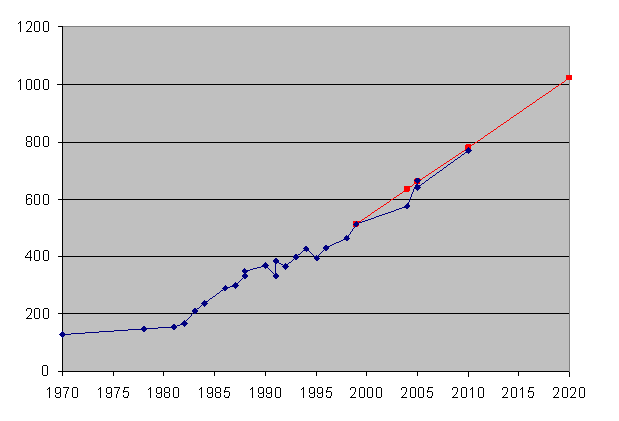
\includegraphics[scale=0.64, clip, viewport=-20 0 680 520]
                {figures/PrognoseRSAFaktorisierungSecorvo.png}
% Parameter von includegraphics: scale, x, y, dx, dy
% dx, dy spezifiziert die Ausdehnung, die man dem Bildes spendiert.
%      Ist dy zu klein, wird das Bild oben abgeschnitten
% x, y sagt, ab wo der Rahmen um das Bild gezeichnet wird.
%      Ist z.B. x=50, sind der linke Rahmenstrich und Teile des linken
%      Teiles des Bildes nicht zu sehen.
% scale dehnt Rahmenlinie und Bild aus -> Sitenrand wird bei 0.7 z.B. kleiner.
}
\caption{Vergleich der publizierten Faktorisierungserfolge (blau) mit der
prognostizierten Entwicklung (rot) [Quelle Fox 2001; letzte Ergänzung 2011]}
\label{secorvo-factorisation-forecast}
\end{center}
\end{figure}




\clearpage  % Erzwingt, dass alle Floating Objekte (z.B. Grafiken VORHER
            % geschrieben werden ! (sonst wurde Kapitel 4.11.4 begonnen,
            % und die Secorvo-Grafik auf er Folgeseite UNTER die Fussnote
            % geschoben. Außerdem wahrscheinlich auch Zeilenumbruch,
            % egal, ob nach der Garfik noch Platz ist.
% ++++++++++++++++++++++++++++++++++++++++++++++++++++++++++++++++++++++++++
\begin{ctsquote}
    Damit das Mögliche entsteht, muss immer wieder das Unmögliche
    versucht werden.
\caption[Hermann Hesse]{Hermann Hesse\footnotemark}
\end{ctsquote}
\addtocounter{footnote}{0}\footnotetext{%
    Hermann Hesse, deutsch-schweizerischer Schriftsteller und Nobelpreisträger,
    02.07.1877$-$09.08.1962.}
% ++++++++++++++++++++++++++++++++++++++++++++++++++++++++++++++++++++++++++

\subsection{Status der Faktorisierung von konkreten großen Zahlen}
\label{nt:NoteFactorization}

Ausführliche Übersichten über die Rekorde im Faktorisieren
zusammengesetzter Zahlen \index{Faktorisierung!Faktorisierungsrekorde}
mit unterschiedlichen Methoden finden sich auf den folgenden Webseiten:
\vspace{-10pt}
\begin{itemize}
\item[]
     %% URL doesn't exist any more in 2018: \url{http://www.crypto-world.com} -- archive.org used below\\
     %% http://primes.utm.edu/glossary/xpage/WheelFactorization.html no overview
     \url{http://primerecords.dk/consecutive_factorizations.htm}\\
     \url{http://en.wikipedia.org/wiki/Integer_factorization_records}\\
     \url{http://en.wikipedia.org/wiki/RSA_Factoring_Challenge}

\end{itemize}

Der aktuelle Rekord (Stand Nov. 2012) mit der GNFS-Methode (General Number
Field Sieve) \index{General Number Field Sieve (GNFS)} zerlegte eine
allgemeine $232$-stellige Dezimalzahl in ihre beiden Primfaktoren.

\vskip +10pt
Die letzten Rekorde\footnote{%
Die  "`RSA-Zahlen"' sind große semiprime Zahlen (d.h. Zahlen, die genau aus
2 Primfaktoren bestehen)\index{Zahlen!semiprim}\index{Primzahl!semiprim}.
Sie wurden von der Firma RSA Security generiert und veröffentlicht: Im
Wettbewerb "`RSA Factoring Challenge"' wurden die Primfaktoren dieser Zahlen gesucht.\\
Siehe \url{http://www.emc.com/emc-plus/rsa-labs/historical/the-rsa-factoring-challenge.htm}.

Die RSA-Laboratorien schreiben ihre Challenges schon seit Anfang der
90er-Jahre aus. In der ersten RSA-Factoring-Challenge wurden die Zahlen, von RSA-100 bis
RSA-500, gemäß der Anzahl ihrer Dezimalstellen benannt; die zweite
RSA-Factoring-Challenge benannte die Zahlen anhand der Anzahl ihrer
Binärstellen. Innerhalb des zweiten Wettbewerbs wurden Geldpreise für die
erfolgreiche Faktorisierung von RSA-576 bis RSA-2048 ausgelobt (RSA-576, RSA-640
etc. in 64-er Schritten --- Die Zahl RSA-617 bildet eine Ausnahme, da sie
vor der Änderung des Namensschemas erzeugt wurde).
Leider beendete RSA Inc. die Challenge vorzeitig und zog die Preise zurück.
Alle noch ungelösten RSA-Challenges der RSA-Labs finden sich inzwischen auch
auf der Webseite des Krypto-Wettbewerbs \glqq MysteryTwister C3\grqq~
(\url{http://www.mysterytwisterc3.org}).
\index{MTC3}\index{Challenge}\index{Cipher-Challenge}\index{Krypto-Wettbewerb}

Die "`C-Zahlen"' stammen aus dem Cunningham-Projekt:
\url{http://homes.cerias.purdue.edu/~ssw/cun/}.
Diese sind Faktoren großer Mersennezahlen, die eine ganz spezielle
Struktur haben. Dies macht es um Größenordnungen einfacher, sie zu
faktorisieren, als Moduli gleicher Längen, die man für RSA erstellt.
                               }
mit Faktorisierungsverfahren für zusammengesetzte Zahlen
sind in Tabelle~\ref{factorizationrecords} aufgeführt.

%% TODO_BE_TODO: Update 2^1193-1 laut https://www.newscientist.com/article/dn26135-factorisation-factory-smashes-number-cracking-record/  und   https://eprint.iacr.org/2014/653
%% See also: http://primes.utm.edu/primes/search.php?Comment=orial&Number=100

\begin{table}[ht]
\begin{center}
\begin{tabular}{|c|ccc@{}c|}
\hline
   & \textbf{Dezimalstellen} & \textbf{Binärstellen} & \textbf{Faktorisiert am} & \textbf{Faktorisiert von}\\
\hline
	&&&&\\
	RSA-768 & 	232 & 768 & Dez 2010 & Thorsten Kleinjung et al.\\
	RSA-200 & 	200 & 663 & Mai 2005 & Jens Franke et al.\\
	RSA-640\footnotemark & 	193 & 640 & Nov 2005 & Jens Franke et al.\\
	RSA-576 & 	174 & 576 & Dez 2003 & Jens Franke et al.\\
	RSA-160 & 	160 & 530 & Apr 2003 & Jens Franke et al.\\
	RSA-155	&	155 & 512 & Aug 1999 & Herman te Riele et al.\\
	\dots & & & &\\
	C307 & 		307 & 1017 & Mai 2007 & Jens Franke et al.\\
	C176 & 		176 & 583 & Mai 2005 & Kazumaro Aoki et al.\\
	C158 & 		158 & 523 & Jan 2002 & Jens Franke et al.\\
\hline
\end{tabular}
\caption{Die derzeitigen Faktorisierungsrekorde (Stand Nov. 2012)}  % Eyecatcher
\label{factorizationrecords}
\end{center}
\end{table}
\footnotetext{%
Eine Arbeitsgruppe des BSI löste die mit 20.000 US-Dollar dotierte Challenge
RSA-640 mit Hilfe der GNFS-Methode. Die Forscher benötigten für die
Zerlegung der Zahl in ihre beiden 320 Bit langen Primfaktoren rund fünf
Monate Rechenzeit.

Die Forscher um Prof. Jens Franke (von der Universität Bonn, dem BSI und dem
CWI) waren nicht auf die Geldpreise aus, sondern wollten die Grenzen der
Forschung ausdehnen. Dadurch werden Aussagen über notwendige Minimallängen
für sichere RSA-Moduli fundierter.
%%% Link unzugänglich: \url{http://www.heise.de/newsticker/meldung/print/65957}
}

%be_2005: Erzwingen, dass die Abb. noch in diesem Kapitel !


Laufzeituntersuchungen zur Faktorisierung\index{Faktorisierung} mit den
Open-Source Software-Paketen Pari-GP, SageMath, CrypTool~1 und CrypTool~2
finden sich in "`Zeitexperimente zur Faktorisierung"' (siehe \cite{Schulz2010}).

\vskip +20pt
%\noindent
Im Folgenden werden die letzten Rekorde aus Tabelle~\ref{factorizationrecords}
etwas ausführlicher erläutert\footnote{%
Die beiden dabei benutzten Methoden GNFS und SNFS werden kurz z.B. auf
den ff. Webseiten dargestellt:
\index{General Number Field Sieve (GNFS)}
\index{Special Number Field Sieve (SNFS)}
\begin{itemize}
\item[]
      \url{http://en.wikipedia.org/wiki/Special_number_field_sieve}\\
      \url{http://en.wikipedia.org/wiki/General_number_field_sieve}
\end{itemize}
\vspace{-10pt}
}:


% --------------------------------------------------------------------------
%\vskip +20pt
\paragraph*{RSA-155} \label{RSA-155} \index{RSA-155}
\mbox{} % Trick: für Zeilenumbruch, da er "//" allein nicht mag ! xxxxxxxxx

Am 22. August 1999 fanden niederländische Forscher die Lösung dieser
RSA-Challenge. Sie zerlegten eine $155$-stellige Zahl in ihre beiden $78$-stelligen
Primfaktoren (vergleiche Kapitel~\ref{chptSecurityParam}).
Mit der $512$ Bit-Zahl RSA-155 war eine {\em magische} Grenze erreicht.



% --------------------------------------------------------------------------
\vskip +20pt
\paragraph*{C158} \label{C158} \index{C158}
\mbox{} % für Zeilenumbruch
\hypertarget{C158-chap3}{}

Am 18. Januar 2002 zerlegten Forscher der Universität Bonn\footnote{%
  \url{https://members.loria.fr/PZimmermann/records/gnfs158}
}
mit der GNFS-Methode (General Number Field Sieve) \index{General Number
Field Sieve (GNFS)} eine $158$-stellige Dezimalzahl in ihre beiden Primfaktoren
(diese haben 73 und 86 Dezimalstellen).

Dieser Rekord fand deutlich weniger Aufmerksamkeit in der Presse als die
Lösung von RSA-155.

Die Aufgabe der Bonner Wissenschaftler entsprang auch nicht einer Challenge,
sondern die Aufgabe war, die letzten Primfaktoren der Zahl $2^{953}+1$
zu finden (siehe~\glqq Wanted List\grqq~des Cunningham-Projekts\index{Cunningham-Projekt}%
\footnote{%
Cunningham-Projekt: \url{http://homes.cerias.purdue.edu/~ssw/cun/}}).

Die 6 kleineren, schon vorher gefundenen Primfaktoren dieser Zahl waren:
$$
\begin{array}{c}
        3, 1907, 425796183929,\\
        1624700279478894385598779655842584377,\\
        3802306738549441324432139091271828121 \quad{\rm und}\\
        128064886830166671444802576129115872060027.
\end{array}
$$
\begin{sloppypar}
Die drei kleinsten Faktoren können leicht\footnote{%
Z.B. mit CT1\index{CT1} über das Menü
\textbf{Einzelverfahren \textbackslash{} RSA-Kryptosystem \textbackslash{}
Faktorisieren einer Zahl}.\\
In sinnvoller Zeit zerlegt CT1 Zahlen bis 250 Bit Länge (Zahlen größer als
1024 Bit werden von CT1 nicht angenommen). CT2\index{CT2} kann auch
Zahlen größer 250 Bit zerlegen.
}
bestimmt werden.
Die nächsten drei Primfaktoren wurden von P.~Zimmermann%
\footnote{\url{http://homepages.loria.fr/PZimmermann/ecmnet/}},
T.~Grandlund und R. Harley in den Jahren 1999 und 2000 mit der Methode
der Elliptischen Kurven gefunden.
\end{sloppypar}

Als letzter Faktor blieb der sogenannte Teiler  "`C158"',
von dem man bis dahin wusste, dass er zusammengesetzt ist, aber man kannte
seine Primfaktoren nicht (die folgenden drei Zeilen sind eine einzige Zahl):
$$
\begin{array}{c}
39505874583265144526419767800614481996020776460304936\\
45413937605157935562652945068360972784246821953509354\\
4305870490251995655335710209799226484977949442955603
\end{array}
$$
Die Faktorisierung von C158 ergab die beiden 73- und 86-stelligen Primfaktoren:
$$
\begin{array}{c}
3388495837466721394368393204672181522815830368604993048084925840555281177
\end{array}
$$
und
$$
\begin{array}{c}
1165882340667125990314837655838327081813101\\
2258146392600439520994131344334162924536139.
\end{array}
$$
Damit wurde die Zahl $2^{953}+1$ vollständig in ihre 8 Primfaktoren zerlegt.

\noindent\begin{minipage}{\textwidth}
\vspace{3ex}
Verweise:
\vspace{-10pt}
\begin{itemize}
\item \url{https://members.loria.fr/PZimmermann/records/gnfs158}
\item \url{https://web.archive.org/web/20170518021747/http://www.crypto-world.com:80/announcements/c158.txt}
        %% original URL doesn't exist any more in 2018:
	%% \url{http://www.crypto-world.com/announcements/c158.txt}
\end{itemize}
\end{minipage}
\vspace{24pt}



% --------------------------------------------------------------------------
\vskip +20pt
\paragraph*{RSA-160} \label{RSA-160} \index{RSA-160}\mbox{}
\hypertarget{RSA-160-chap3}{}

Am 1. April 2003 zerlegten Forscher der Universität Bonn\footnote{%
          \url{https://members.loria.fr/PZimmermann/records/rsa160}\\
          \url{https://members.loria.fr/PZimmermann/records/factor.html}\\
          \url{https://web.archive.org/web/20170518021747/http://www.crypto-world.com:80/FactorWorld.html}
          %% \url{http://www.crypto-world.com/FactorWorld.html}
}
mit der GNFS-Methode (General Number Field Sieve) \index{General Number
Field Sieve (GNFS)} eine $160$-stellige Zahl in ihre beiden Primfaktoren
(diese haben jeweils 80 Dezimalstellen).

Die Berechnungen dazu fanden auch im Bundesamt für Sicherheit in der
Informationstechnik (BSI) in Bonn statt.\footnote{%
Das BSI \index{BSI} erstellt jedes Jahr ein Papier über die Eignung von
Kryptoalgorithmen, mit denen Signaturen erzeugt werden können,
die den Vorgaben des deutschen Signaturgesetzes genügen.
Bei dieser Erstellung werden Experten aus Wirtschaft und Wissenschaft
beteiligt. Um die Eignung von Signaturverfahren zu beurteilen, deren
Schwierigkeit auf dem Faktorisierungsproblem beruht,
kooperiert das BSI auch mit Forschern der Universität Bonn.
%%% Toter Link: \url{http://www.bsi.bund.de/esig/basics/techbas/krypto/index.htm}
}

Die 160-stellige Dezimalzahl stammt von der alten Challenge-Liste von RSADSI.
Diese wurde nach der Faktorisierung von RSA-155 (RSA512) zurückgezogen.
Die Primfaktoren von RSA-160 waren aber nicht bekannt.
Deshalb ist dieser Rekord von Prof.\ Frankes Team immer noch die Lösung
einer alten Challenge, für die es aber von RSADSI kein Geld gibt.

Die zusammengesetzte Zahl "`RSA-160"' lautet (die folgenden drei Zeilen
sind eine einzige Zahl):
$$
\begin{array}{c}
215274110271888970189601520131282542925777358884567598017049\\
767677813314521885913567301105977349105960249790711158521430\\
2079314665202840140619946994927570407753
\end{array}
$$
Die Faktorisierung von RSA-160 ergab die beiden Primfaktoren:
$$
\begin{array}{c}
p = 45427892858481394071686190649738831\\
    656137145778469793250959984709250004157335359
\end{array}
$$
und
$$
\begin{array}{c}
q = 47388090603832016196633832303788951\\
    973268922921040957944741354648812028493909367
\end{array}
$$

Die Berechnungen erfolgten zwischen Dezember 2002 und April 2003.
\vspace{24pt}



% ammmmmmmmmmma
%
% RSA-576 faktorisiert
% Am 27.04.2004 ging die Nachricht durch
% die Ticker, dass die 576-bit-Challenge der
% Firma RSA gelöst sei. Tatsächlich wurde
% die 174 Dezimalstellen lange Zahl bereits
% am 03.12.2003 zerlegt. Die Faktorisierung
% gelang einem Team der Universität Bonn
% um Professor Franke mit Unterstützung
% durch das Institut für Experimentelle Mathematik
% in Essen und das BSI. Die verteilte
% Berechung erfolge auf einem Linux-
% Cluster mit 144 PCs (400 MHz, Pentium II)
% und verwendete den General Number Field
% Sieve-Algorithmus ? mit einem Aufwand
% von umgerechnet 13.200 MIPS-Jahren.
% Interessant dabei: Dieser Faktorisierungserfolg
% bestätigt die Prognose, die Secorvo
% vor drei Jahren auf der Basis der Faktorisierungserfolge
% der vergangenen 30 Jahre
% gestellt hat (siehe Bild), und die weit weniger
% dramatisch ausfiel als viele Expertenwarnungen
% und die Erwartung des BSI.
% Danach wäre 2004 erstmals die Faktorisierung
% einer 630 bit langen Zahl zu erwarten
% gewesen ? was nun eher unwahrscheinlich
% erscheint. Selbst die frühestens für das
% Jahr 2020 vorausgesagte Faktorisierung
% eines 1024 bit langen RSA-Schlüssels
% könnte sich daher noch als zu pessimistische
% Befürchtung erweisen ? allen Warnern
% zum Trotz, die seit Jahren Schlüssell
% ängen von 2048 bit und mehr empfehlen
% oder gar das baldige Ende von RSA prophezeihen.
%
% ammmmmmmmmmmz




% --------------------------------------------------------------------------
\vskip +20pt
\hypertarget{RSA-200-chap3}{}
\paragraph*{RSA-200} \label{RSA-200} \index{RSA-200}\mbox{}
\nopagebreak

Am 9. Mai 2005 meldete die Forschergruppe von Prof. Jens Franke der Universität Bonn\footnote{%
   \url{https://members.loria.fr/PZimmermann/records/rsa200}
   },
dass sie gemeinsam mit Kollegen des Amsterdam Centrum voor Wiskunde en Informatica
einen neuen Weltrekord im Faktorisieren aufstellten.

Sie zerlegten mit der GNFS-Methode (General Number Field Sieve) \index{General Number
Field Sieve (GNFS)} eine $200$-stellige Zahl in ihre beiden Primfaktoren
(diese haben jeweils 100 Dezimalstellen).

Die zusammengesetzte Zahl "`RSA-200"' lautet (die folgenden drei Zeilen
sind eine einzige Zahl):
$$
\begin{array}{c}
2799783391122132787082946763872260162107044678695542853756000992932\\
6128400107609345671052955360856061822351910951365788637105954482006\\
576775098580557613579098734950144178863178946295187237869221823983
\end{array}
$$
Die Faktorisierung von RSA-200 ergab die beiden Primfaktoren:
$$
\begin{array}{c}
p = 35324619344027701212726049781984643686711974001976\\
    25023649303468776121253679423200058547956528088349
\end{array}
$$
und
$$
\begin{array}{c}
q = 79258699544783330333470858414800596877379758573642\\
    19960734330341455767872818152135381409304740185467
\end{array}
$$

Die Berechnungen erfolgten zwischen Dezember 2003 und Mai 2005.
Die Faktorisierung durch die Gruppe um Bahr, Böhm, Franke, Kleinjung,
Montgomery und te Riele hatte also knapp 17 Monate gedauert.
Der Rechenaufwand lag bei umgerechnet etwa 120.000 MIPS-Jahren\footnote{%
Ein MIPS-Jahr (MY) ist die Anzahl von Operationen, die eine Maschine,
welche eine Million Integeroperationen pro Sekunde (MIPS)
ausführt, in einem Jahr bewältigt. Zur Illustration: ein INTEL
Pentium 100 Prozessor hat etwa 50 MIPS.
Für die Zerlegung eines 2048-Bit-Moduls bräuchte man ca. {$8,5 \cdot
10^{40}$ MY}.}.
\vspace{24pt}




% --------------------------------------------------------------------------
\vskip +20pt
\hypertarget{RSA-768-chap3}{}
\paragraph*{RSA-768} \label{RSA-768} \index{RSA-768}\mbox{}
\nopagebreak

Am 12. Dezember 2009 meldete die Forschergruppe um Prof. Thorsten
Kleinjung\footnote{%
   \url{http://eprint.iacr.org/2010/006.pdf} \cite{Kleinjung2010}
          }, dass sie
eine $232$-stellige Zahl in ihre beiden Primfaktoren zerlegten
(diese haben jeweils 116 Dezimalstellen).
Sie benutzten dazu die GNFS-Methode (General Number Field Sieve)
\index{General Number Field Sieve (GNFS)} in einer Art, dass vor dem
Matrix-Schritt auf mehreren hundert Rechnern "`Oversieving"' betrieben wurde.

Die zusammengesetzte Zahl "`RSA-768"' lautet (die folgenden drei Zeilen
sind eine einzige Zahl):
$$
\begin{array}{c}
123018668453011775513049495838496272077285356959533479219732245215172640050726\\
365751874520219978646938995647494277406384592519255732630345373154826850791702\\
6122142913461670429214311602221240479274737794080665351419597459856902143413
\end{array}
$$
Die Faktorisierung von RSA-768 ergab die beiden Primfaktoren (je 384 bit):
$$
\begin{array}{c}
p = 3347807169895689878604416984821269081770479498371376856891\\
    2431388982883793878002287614711652531743087737814467999489
\end{array}
$$
und
$$
\begin{array}{c}
q = 3674604366679959042824463379962795263227915816434308764267\\
    6032283815739666511279233373417143396810270092798736308917
\end{array}
$$

Die Berechnungen dauerten 2 1/2 Jahre.\footnote{%
Dies war ein "`academic effort"' -- Organisationen mit besserer Ressourcen-Ausstattung
könnten es deutlich schneller durchführen.}
\vspace{24pt}





% --------------------------------------------------------------------------
\vskip +20pt
\paragraph*{C307 / M1039} \label{C307} \index{C307} \index{M1039}
\mbox{} % für Zeilenumbruch
\hypertarget{C307-chap3}{}

Im Mai 2007 meldeten Prof. Franke, Prof. Kleinjung (von der Universität Bonn),
das japanische Telekommunikationsunternehmen NTT und Prof. Arjen Lenstra von
der Polytechnischen Hochschule in Lausanne, dass sie mit der SNFS-Methode
(Special Number Field Sieve) \index{Special Number Field Sieve (SNFS)}
innerhalb von 11 Monaten eine $307$-stellige Dezimalzahl in ihre beiden
Primfaktoren zerlegten (diese haben 80 und 227 Dezimalstellen).

Die Aufgabe der Wissenschaftler entsprang nicht einer Challenge, sondern
die Aufgabe war, die letzten Primfaktoren der Mersenne-Zahl $2^{1039}+1$
zu finden (siehe~ \glqq Wanted List\grqq~ des Cunningham-Projekts\index{Cunningham-Projekt}%
\footnote{%
Cunningham-Projekt: \url{http://homes.cerias.purdue.edu/~ssw/cun/}\\
% BE_18-8-8: Link tot: Cunningham-Tabelle: \url{http://homes.cerias.purdue.edu/~ssw/cun/pmain1215}\\%%%Linkänderungen: 1206-> 1215 -> 135
Die Zahlen in der Cunningham-Tabelle werden folgendermaßen geschrieben:\\
\glqq (2,n)-\grqq~ bedeutet $2^{n}-1$;~~~
\glqq (2,n)+\grqq~ bedeutet $2^{n}+1$.\\
Um die Größenordnung einer Zerlegung anzudeuten schreibt man $p<n>$ oder $c<n>$,
wobei \glqq n\grqq~ die Anzahl der Dezimalstellen ist und \glqq p\grqq~ und \glqq c\grqq~
bedeuten, dass die Zahl eine Primzahl oder eine zusammengesetzte Zahl ist.\\
$2^{1039}-1 = p7 * c307 = p7 * p80 * p227$\\
Genauer erklärt wird dies auf der Seite zum Cunningham-Projekt:\\
\glqq 2,651+ means $2^{651} + 1$ and the size (c209 means 209 decimal digits)
of the
number which was factored.  Then come the new factor(s), the discoverer and
the method used.  Recently, only the multiple polynomial quadratic sieve
(ppmpqs), the elliptic curve method (ecm) and the number field sieve (nfs)
have been used.  `hmpqs' stands for hypercube multiple polynomial quadratic
sieve.  Under `new factors', `p90' means a 90-digit prime and `c201' is a
201-digit composite number.\grqq.
}).\\


Die Zahl $2^{1039}-1$ besteht aus 3 Primfaktoren: Der kleinste Faktor
$p7 = 5080711$ war schon länger bekannt.\footnote{%
  Er kann mit CT1\index{CT1} über das Menü
  \textbf{Einzelverfahren \textbackslash{} RSA-Kryptosystem \textbackslash{}
  Faktorisieren einer Zahl} gefunden werden --- mit den Algorithmen von Brent,
  Williams oder Lenstra, mit denen man gut \glqq relativ\grqq~ kleine Faktoren
  abspalten kann. Analog geht es in CT2\index{CT2} mit der Komponente
  GeneralFactorizer.
}

Zur vollständigen Faktorisierung musste der zweite Faktor (Koteiler) "`C307"'
zerlegt werden: Bis dahin wusste man nur, dass er zusammengesetzt ist, aber man
kannte weder die Anzahl seiner Primfaktoren, noch die Primfaktoren selbst.
Die folgenden fünf Zeilen sind eine einzige Zahl:
$$
\begin{array}{c}
C307 =1159420574072573064369807148876894640753899791702017724986868353538\\
8224838599667566080006095408005179472053993261230204874402860435302\\
8619141014409345351233471273967988850226307575280937916602855510550\\
0425810771176177610094137970787973806187008437777186828680889844712\\
822002935201806074755451541370711023817
\end{array}
$$
Die Faktorisierung von C307 ergab die beiden 80- und 227-stelligen Primfaktoren:
$$
\begin{array}{c}
p80 = 558536666199362912607492046583159449686465270184\\
      88637648010052346319853288374753
\end{array}
$$
und
$$
\begin{array}{c}
p227 = 207581819464423827645704813703594695162939708007395209881208\\
       387037927290903246793823431438841448348825340533447691122230\\
       281583276965253760914101891052419938993341097116243589620659\\
       72167481161749004803659735573409253205425523689
.
\end{array}
$$
Damit wurde die Zahl $2^{1039}-1$ vollständig in ihre 3 Primfaktoren zerlegt.

\noindent\begin{minipage}{\textwidth}
\vspace{3ex}
Verweise:
\vspace{-10pt}
\begin{itemize}
\item \url{http://www.loria.fr/~zimmerma/records/21039-}
\item \url{https://web.archive.org/web/20170518021747/http://www.crypto-world.com:80/announcements/m1039.txt}
\item \url{https://web.archive.org/web/20170518024506/http://www.crypto-world.com:80/FactorAnnouncements.html}
\end{itemize}
\end{minipage}






% --------------------------------------------------------------------------
\vskip +50pt
\paragraph*{Größenordnung faktorisierter Zahlen im Vergleich zu auf Primalität
getesteter Zahlen}
\mbox{}

Wie man sieht, sind die größten (aus 2 Primfaktoren) zusammengesetzten
Zahlen, die man faktorisieren kann, deutlich kleiner als die Zahlen mit
einer speziellen Struktur, für die Primzahltests\index{Primzahltest} in
der Lage sind, Aussagen über ihre Primalität zu treffen (siehe Kapitel
\ref{search_for_very_big_primes},~\ref{primality_tests} und
\ref{spezialzahlentypen}).


% be_2005_UPDATEN_if-new-mersenne-prime-appears   % Eyecatcher_neue-Mersenne
Länge der derzeitigen Weltrekorde in Dezimaldarstellung:

$$  ~~~~~~~~~[RSA{-}768{-}Zahl] ~~\longleftrightarrow{}~~[49.~bekannte~Mersenne~Primzahl] $$
$$ 232 ~~ \longleftrightarrow{} ~~ 22.338.618 ~~~~~$$
$$ [vgl.~Tab.~\ref{factorizationrecords}] ~~\longleftrightarrow{}~~ [vgl.~Tab.~\ref{L_n_Largest_Known-Primes}] ~~~~~~~~~~~~~~~~$$

%be_2005 - erzwungenes Blank und $$ um Pfeilzeichen, sonst setzt er Blanks an
%          die falschen Stellen.
%        - Wenn man hier \~ statt nur ~ (außerhalb der $$) schreibt, kommen
%          nachher Fussnoten mit
%          \textbf{Einzelverfahren \textbackslash{} Protokolle}
%          nur noch mit kaputten Schriftzeichen raus !



% --------------------------------------------------------------------------
\vskip +60pt
\subsection[Weitere Forschungsergebnisse zu Primzahlen und Faktorisierung]
           {Weitere Forschungsergebnisse zu Primzahlen und Faktorisie"-rung}
\label{FactorisationResearch}
Primzahlen sind Teil vieler hochaktueller Forschungsgebiete der Zahlentheorie.
Die Fortschritte bei der Faktorisierung sind größer als noch in 2005
geschätzt -- sie gehen nicht nur auf das Konto schnellerer Rechner,
sondern sie sind auch in neuen mathematischen Erkenntnissen begründet.
Der aktuelle Stand der Forschung wird dikutiert in Kapitel \ref{Chapter_Dlog-FactoringDead}.

Die Sicherheit des RSA-Algorithmus basiert auf der empirischen Beobachtung,
dass die Faktorisierung großer ganzer Zahlen ein schwieriges Problem ist.
Besteht wie beim RSA-Algorithmus der zugrunde liegende Modul $n$ aus dem Produkt
zweier großer Primzahlen $p, q$ (typische Längen: $p, q$  $500-600$ bit,
$n$ $1024$ bit), so lässt sich $n=pq$ aus $p$ und $q$ leicht bestimmen,
jedoch ist es mit den bisher bekannten Faktorisierungsalgorithmen nicht
möglich, umgekehrt $p, q$ aus $n$ zu gewinnen.
Um jedoch den privaten aus dem öffentlichen Schlüssel zu ermitteln,
bräuchte man entweder Kenntnis von $p$ und $q$ oder vom Wert der
Eulerschen Phi-Funktion\index{Eulersche Phi-Funktion} $\phi(n)$.

Die Entdeckung eines Algorithmus zur effizienten Faktorisierung von
Produkten $n=pq$ großer Primzahlen würde daher den RSA-Algorithmus
wesentlich beeinträchtigen. Je nach Effizienz der Faktorisierung im
Vergleich zur Erzeugung von $p, q, n$ müsste der verwendete Modul $n$
(z.Zt. 1024 bit) erheblich vergrößert oder --- im Extremfall --- auf
den Einsatz des RSA ganz verzichtet werden.


% --------------------------------------------------------------------------
\vskip +20pt
%\paragraph*
\subsubsection{Das Papier von Bernstein und seine Auswirkungen auf die Sicherheit
               des RSA-Algorithmus}
\label{RSABernstein} \index{Faktorisierung!Faktorisierungsproblem}
%\mbox{} % für Zeilenumbruch, da er \\ allein nicht mag !
        % Braucht die Leerzeile danach auch noch !! bebebe ?
Die im November 2001 veröffentlichte Arbeit \glqq Circuits for integer
factorization: a proposal\grqq~von D.J. Bernstein \cite{Bernstein2001}
behandelt das Problem der Faktorisierung großer Zahlen.
Die Kernaussage des Papers besteht darin, dass es möglich ist, die
Implementierung des General Number Field Sieve-Algorithmus (GNFS)
\index{General Number Field Sieve (GNFS)} so zu
verbessern, dass mit gleichem Aufwand wie bisher Zahlen mit 3-mal
größerer Stellenzahl (Bit-Länge) faktorisiert werden können.

Wesentlich bei der Interpretation des Resultats ist die Definition des
Aufwandes: Als Auf"-wand wird das Produkt von benötigter Rechenzeit und
Kosten der Maschine (insbesondere des verwendeten Speicherplatzes)
angesetzt. Zentral für das Ergebnis des Papiers ist die Beobachtung, dass
ein wesentlicher Teil der Faktorisierung auf Sortierung zurückgeführt
werden kann und mit dem Schimmlerschen Sortierschema ein Algorithmus zur
Verfügung steht, der sich besonders gut für den Einsatz von
Parallelrechnern eignet. Am Ende des Abschnittes 3 gibt Bernstein konkret
an, dass die Verwendung von $m^2$ Parallelrechnern mit jeweils gleicher
Menge an Speicherplatz mit Kosten in der Größenordnung von $m^2$
einhergeht --- genau so wie ein einzelner Rechner mit $m^2$ Speicherzellen.
Der Parallelrechner bewältigt die Sortierung von $m^2$ Zahlen jedoch
(unter Verwendung der o.~g.\ Sortierverfahrens) in Zeit proportional zu m,
wohingegen der Einprozessorrechner Zeit proportional $m^2$ benötigt.
Verringert man daher den verwendeten Speicherplatz und erhöht --- bei
insgesamt gleich bleibenden Kosten --- die Anzahl der Prozessoren
entsprechend, verringert sich die benötigte Zeit um die Größenordnung
$1/m$. In Abschnitt 5 wird ferner angeführt, dass der massive Einsatz der
parallelisierten Elliptic Curve-Methode von Lenstra die Kosten der
Faktorisierung ebenfalls um eine Größenordnung verringert (ein
Suchalgorithmus hat dann quadratische statt kubische Kosten).  Alle
Ergebnisse von Bernstein gelten nur asymptotisch für große Zahlen $n$.
Leider liegen keine Abschätzungen über den Fehlerterm, d.h.  die
Abweichung der tatsächlichen Zeit von dem asymptotischen Wert, vor --- ein
Mangel, den auch Bernstein in seinem Papier erwähnt. Daher kann zur Zeit
keine Aussage getroffen werden, ob die Kosten (im Sinne der Bernsteinschen
Definition) bei der Faktorisierung z.~Zt.\ verwendeter RSA-Zahlen
(1024$-$2048 bit) bereits signifikant sinken würden.

Zusammenfassend lässt sich sagen, dass der Ansatz von Bernstein durchaus
innovativ ist. Da die Verbesserung der
Rechenzeit unter gleichbleibenden Kosten durch einen massiven Einsatz von
Parallelrechnern erkauft wird, stellt sich die
Frage nach der praktischen Relevanz. Auch wenn formal der Einsatz von einem
Rechner über 1 sec  und  1.000.000 Rechnern
für je 1/1.000.000 sec dieselben Kosten erzeugen mag, ist die
Parallelschaltung von 1.000.000 Rechnern praktisch nicht
(oder nur unter immensen Fixkosten, insbesondere für die Vernetzung der
Prozessoren) zu realisieren. Solche Fixkosten
werden aber nicht in Ansatz gebracht.
Die Verwendung verteilter Ansätze (distributed computing) über ein
großes Netzwerk könnte einen Ausweg bieten. Auch hier müssten
Zeiten und Kosten für Datenübertragung einkalkuliert werden.

Solange noch keine (kostengünstige) Hardware oder verteilte Ansätze
entwickelt wurden, die auf
dem Bernsteinschen Prinzip basieren, besteht noch keine akute Gefährdung
des RSA. Es bleibt zu klären, ab welchen
Größenordnungen von n die Asymptotik greift.

Arjen Lenstra, Adi Shamir et.~al.\ haben das Bernstein-Paper analysiert
\cite{Lenstra2002}.
Als Ergebnis kommen Sie zu einer Bitlängen-Verbesserung der
Faktorisierung um den Faktor 1.17
(anstatt Faktor 3 wie von Bernstein erwartet).

Die Zusammenfassung ihres Papers \glqq Analysis of Bernstein's Factorization
Circuit\grqq~lautet:

\glqq ... Bernstein proposed a circuit-based implementation of
the matrix step of the number field sieve factorization algorithm. We
show that under the non-standard cost function used in [1], these circuits
indeed offer an asymptotic improvement over other methods but
to a lesser degree than previously claimed: for a given cost, the new
method can factor integers that are 1.17 times larger (rather than 3.01).
We also propose an improved circuit design based on a new mesh routing
algorithm, and show that for factorization of 1024-bit integers the
matrix step can, under an optimistic assumption about the matrix size,
be completed within a day by a device that costs a few thousand dollars.
We conclude that from a practical standpoint, the security of RSA relies
exclusively on the hardness of the relation collection step of the number
field sieve.\grqq

Auch RSA Security kommt in ihrer
Analyse der Bernstein-Arbeit \cite{RSA-Security2002} vom 8. April 2002
erwartungsgemäß zu dem Ergebnis, dass RSA weiterhin als ungebrochen betrachtet
werden kann.

Die Diskussion ist weiterhin im Gang.

Zum Zeitpunkt der Erstellung dieses Absatzes (Juni 2002) war nichts
darüber bekannt, inwieweit die im Bernstein-Papier vorgeschlagenen
theoretischen Ansätze realisiert wurden oder wieweit die Finanzierung
seines Forschungsprojektes ist.
%%
%% \noindent\begin{minipage}{\textwidth}
%% \vspace{3ex}
%% Verweise:
%% \vspace{-10pt}
%% \begin{itemize}
%%   \item[] \url{http://cr.yp.to/djb.html}\\
%%           %% Link tot: \url{http://www.counterpane.com/crypto-gram-0203.html\#6}\\
%%           %% Link zu generisch: \url{http://www.math.uic.edu}
%% \end{itemize}
%% \end{minipage}



% --------------------------------------------------------------------------
\vskip +20pt
%\paragraph*
\subsubsection{Das TWIRL-Device} \label{TWIRLDevice} \index{TWIRL-Device}
%\mbox{} % Trick: für Zeilenumbruch

Im Januar 2003 veröffentlichten Adi Shamir und Eran Tromer vom Weizmann
Institute of Science den vorläufigen Draft {\em \glqq Factoring Large Numbers
with the TWIRL Device\grqq}, in dem deutliche Bedenken gegen RSA-Schlüssellängen
unter 1024 begründet werden \cite{Shamir2003}.

Das Abstract fasst ihre Ergebnisse folgendermaßen zusammen: \glqq The security of the RSA cryptosystem depends on the difficulty of factoring large integers. The best current factoring algorithm is the Number Field Sieve (NFS), and its most difficult part is the sieving step. In 1999 a large distributed computation involving thousands of workstations working for many months managed to factor a 512-bit RSA key, but 1024-bit keys were believed to be safe for the next 15-20 years. In this paper we describe a new hardware implementation of the NFS sieving step ... which is 3-4 orders of magnitude more cost effective than the best previously published designs ... . Based on a detailed analysis of all the critical components (but without an actual implementation), we believe that the NFS sieving step for 1024-bit RSA keys can be completed in less than a year by a \$10M device, and that the NFS sieving step for 512-bit RSA keys can be completed in less than ten minutes by a \$10K device. Coupled with recent results about the difficulty of the NFS matrix step ... this raises some concerns about the security of these key sizes.\grqq

Eine ausführliche Fassung findet sich auch in dem Artikel der beiden Autoren
in den RSA Laboratories CryptoBytes \cite{Shamir2003a}.

Eine sehr gute Erläuterung, wie der Angriff mit dem Generalized Number Field
Sieve (GNFS) \index{General Number Field Sieve (GNFS)} funktioniert und
welche Fortschritte sich ergaben, findet sich
in dem 3-seitigen Artikel in der DuD-Ausgabe Juni/2003 \cite{Weis2003}.
Beim GNFS können 2 grundlegende Schritte unterschieden werden:
der Siebungsschritt (Relationen sammeln) und die Matrix-Reduktion.
Auch wenn der Siebungsschritt hochgradig parallelisierbar ist, so dominiert
er doch den Gesamtrechenaufwand. Bisher haben Shamir und Tromer noch kein
TWIRL-Device gebaut, jedoch ist der dafür ge"-schätzte Aufwand von 10 bis
50 Millionen Euro, um eine 1024-Bit Zahl in einem Jahr zu faktorisieren
für Geheimdienste oder große kriminelle Organisationen keineswegs prohibitiv,
denn die \glqq Kosten für einen einzigen Spionagesatelliten schätzt man
z.B. auf mehrere Milliarden USD\grqq. Die Autoren empfehlen deshalb konkret,
möglichst rasch sensible, bisher benutzte RSA-, Diffie-Hellman- oder
ElGamal-Schlüssel von bis zu 1024 Bit zu wechseln und Schlüssel von
mindestens 2048 Bit Länge einzusetzen.
Auch für die geplante TCPA/Palladium-Hardware \index{Palladium} werden
2048-Bit RSA-Schlüssel verwendet!

Damit erscheinen die aktuellen Empfehlungen des BSI, auf längere
RSA-Schlüssellängen umzustellen, mehr als gerechtfertigt.



% --------------------------------------------------------------------------
\vskip +20pt
%\paragraph*{``Primes in P'': Testen auf Primalität ist polynominal}
\subsubsection{\glqq Primes in P\grqq: Testen auf Primalität ist polynominal}
\label{PrimesinP} \index{Primzahltest}
%\mbox{} % für Zeilenumbruch, da er // allein nicht mag ! xxxxxxxxx

Im August 2002 veröffentlichten die drei indischen Forscher M. Agrawal,
N. Kayal und N. Saxena ihr Paper {\em \glqq PRIMES in P\grqq}  %{\em ``PRIMES in P''}
über einen neuen Primzahltest-Algorithmus, genannt AKS\index{AKS} \cite{Agrawal2002}.
Sie entdeckten einen polynominalen\index{Polynom} deterministischen Algorithmus, um zu entscheiden, ob eine gegebene Zahl prim ist oder nicht.

Die Bedeutung dieser Entdeckung liegt darin, dass sie Zahlentheoretiker mit neuen Einsichten und Möglichkeiten für die weitere Forschung versorgt. Viele Menschen haben im Lauf der Jahrhunderte nach einem polynominalen Primzahltest gesucht, so dass dieses Ergebnis einen theoretischen Durchbruch darstellt. Es zeigt sich immer wieder, dass aus schon lange bekannten Fakten neue Ergebnisse generiert werden können.

Aber selbst die Autoren merken an, dass andere bekannte Algorithmen (z.B. ECPP) schneller sein können. Der neue Algorithmus funktioniert für alle positiven ganzen Zahlen. Dagegen verwendet das GIMPS-Projekt den Lucas-Lehmer-Primzahltest, der besondere Eigenschaften der Mersennezahlen ausnutzt. Dadurch ist der Lucas-Lehmer-Test viel schneller und erlaubt, Zahlen mit Millionen von Stellen zu testen, während generische Algorithmen auf Zahlen mit einigen tausend Stellen beschränkt sind. Nachteil der bisherigen schnellen Verfahren ist, dass sie probabilistisch sind, also ihr Ergebnis höchstwahrscheinlich, aber nicht ganz sicher ist.

\enlargethispage{20pt}
\noindent Aktuelle Forschungsergebnisse dazu finden sich z.B. auf:
\vspace{-10pt}
\begin{itemize}
  \item[] \url{http://www.mersenne.org/}\\
          \url{http://fatphil.org/maths/AKS/} Originaltext in Englisch
          % BE_2018 Toter Link: \href{http://ls2-www.cs.uni-dortmund.de/lehre/winter200203/kt/material/primes.ps}{\tt http://ls2-www.cs.uni-dortmund.de/lehre/winter200203/kt/material/primes.ps}\\% \url... created overfull \hbox
          % BE_2018  \hspace*{2em}\hspace*{2em}Gute Erläuterung in Deutsch von Thomas Hofmeister.
\end{itemize}
\vskip +10 pt



% --------------------------------------------------------------------------
\vskip +20pt
\subsubsection{\glqq Shared Primes\grqq: Module mit gleichen Primfaktoren}
\label{nt_Shared-Primes} \index{Primzahl!Shared}
%~\ref{nt_Shared-Primes}, S.~\pageref{nt_Shared-Primes}

Der RSA-Algorithmus basiert auf der angenommenen Schwierigkeit, große semi-prime
natürliche Zahlen (Module) zu faktorisieren (Faktorisierungsproblem).
Wie Lenstra et al \cite{Lenstra2012} beschrieben, ist es aber möglich, aus
einer gegebenen Menge von Modulen einige zu faktorisieren, sofern sie
gemeinsame Primfaktoren (shared primes) aufweisen. In diesem Fall kann das
Faktorisierungsproblem umgangen werden, indem man die -- relativ einfach zu
berechnenden -- größten gemeinsamen Teiler (ggT) bestimmt. Andererseits ist es
keine triviale Aufgabe, alle Shared Primes (gemeinsame Primfaktoren) effizient
zu bestimmen und die zugehörigen Module zu faktorisieren, wenn die gegebene
Menge von Moduln sehr groß ist (mehrere Millionen).

Die ggTs lassen sich nur nutzen, wenn die RSA-Schlüssel nicht zufällig genug
erzeugt wurden. Zieht man die Wichtigkeit starker kryptographischer Schlüssel
in Betracht, sollte man verifizieren, dass alle Schlüssel (wirklich)
zufällig erzeugt wurden \cite{Esslinger2012}.

Als Lenstra et al ihr Paper \cite{Lenstra2012} im Februar 2012
veröffentlichten, veröffentlichten sie nicht den zugehörigen Source-Code.
Kurz danach wurde der Source-Code eines ähnlichen Programms auf der
CrypTool-Website\footnote{%
\url{http://www.cryptool.org/de/ctp-dokumentation-de/361-ctp-paper-rsa-moduli}
}
in Python\index{Python} und C++ veröffentlicht, und noch etwas später auf der Seite, die von
\cite{Heninger2012}\footnote{\url{https://www.factorable.net/}
} benutzt wurde.
Der schnellste bisher bekannte Code ist von \cite{Heninger2012}.

Diese Programme finden alle eventuell existierenden gemeinsamen Primfaktoren aus
einer gegebenen Menge von Modulen, auch wenn diese Menge Millionen von
Modulen enthält. Mit diesen Programmen können dann System-Administratoren ihre
eigenen RSA-Schlüssel testen.

Der einfachste Ansatz, alle Primfaktoren zu finden (indem man jeden Modul mit
jedem anderen vergleicht), hat eine Komplexität, die quadratisch mit der Anzahl
der Modulen wächst.

Eine sehr effiziente Methode, die Bäume zum Vergleich aller ggT-Paare benutzt,
basiert auf einer Publikation von Dan Bernstein aus 2005 \cite{Bernstein2005}. Bernstein benutzt eine Vorberechnung, in der das Produkt aller Module erzeugt wird. Das ist ein weiteres Beispiel dafür, wie hilfreich Vorberechnungen sein können, um kryptographische Systeme zu brechen (ein anderes berühmtes Beispiel sind die Rainbow-Tabellen, um die Ursprungswerte von Hashwertes zu finden \cite{Oechslin2003}).


Das folgende SageMath-Beispiel zeigt die sehr unterschiedlichen Laufzeiten für die Berechnung eines ggT und einer Faktorisierung. In dem Abschnitt nach diesem Beispiel wird der Kern der Methode erklärt, der in \cite{Heninger2012} benutzt wird: Die Benutzung von zwei Bäumen beschleunigt die Berechnung deutlich.

Das SageMath-Beispiel~\ref{nt_sagesample_Compare-Runtime-gcd-factoring} zeigt, dass die folgenden Operationen sehr schnell sind: Multiplikation von Faktoren, Dividieren eines Moduls durch einen bekannten Faktor und Berechnen des ggT. Im Gegensatz dazu steigt die Rechendauer zur Faktorisierung von längeren Moduli stark an. Selbst die relativ kleinen Module in diesem Beispiel zeigen das: Der kleinere Modul (69 Dezimalstellen, 228 bit) brauchte 76 Sekunden, während der größere (72 Dezimalstellen, 239 bit) schon fast 217 Sekunden benötigte.

Hinzu kommt, dass die Operationen Multiplikation, Division und ggT große Laufzeit-Unter"-schiede aufweisen, wenn die Operanden von sehr unterschiedlicher Größe sind.

% Just to show the origin of the used primes
% sage: factor (2^211-1)
% 15193 * 60272956433838849161 * 3593875704495823757388199894268773153439
%
% sage: factor (2^214-1)
% 3 * 643 * 84115747449047881488635567801 * 162259276829213363391578010288127
\begin{sagecode}
\begin{Verbatim}%
[fontsize=\footnotesize]

# Multiplication
sage: 3593875704495823757388199894268773153439 * 84115747449047881488635567801
302301541122639745170382530168903859625492057067780948293331060817639

sage: 3593875704495823757388199894268773153439 * 162259276829213363391578010288127
583139672825572068433667900695808357466165186436234672858047078770918753


# Division
sage: time 302301541122639745170382530168903859625492057067780948293331060817639 /
           3593875704495823757388199894268773153439
Wall time: 0.00 s
84115747449047881488635567801

sage: time 583139672825572068433667900695808357466165186436234672858047078770918753 /
           3593875704495823757388199894268773153439
Wall time: 0.00 s
162259276829213363391578010288127


# Calculate gcd
sage: time gcd (583139672825572068433667900695808357466165186436234672858047078770918753,
                302301541122639745170382530168903859625492057067780948293331060817639)
Wall time: 0.00 s
3593875704495823757388199894268773153439


# Factorize
sage: time factor (583139672825572068433667900695808357466165186436234672858047078770918753)
Wall time: 217.08 s
162259276829213363391578010288127 * 3593875704495823757388199894268773153439

sage: time factor (302301541122639745170382530168903859625492057067780948293331060817639)
Wall time: 76.85 s
84115747449047881488635567801 * 3593875704495823757388199894268773153439

\end{Verbatim}
\caption{Vergleich der Laufzeit bei der Berechnung eines ggT und einer Faktorisierung}
\label{nt_sagesample_Compare-Runtime-gcd-factoring}
\end{sagecode}



\clearpage
\section*{Effiziente Berechnung aller ggT-Paare und Erläuterung der benutzten Formel zur Bestimmung der Shared Primes}

Der hervorragende Artikel \glqq Mining Your Ps and Qs: Detection of Widespread Weak Keys in Network Devices\grqq~\cite{Heninger2012} erklärt, wie der Algorithmus die ggTs von allen RSA-Moduln effizient berechnet.

Zuerst wird das Produkt $P$ aller Moduln $m_{i}$ mit Hilfe eines Produktbaumes berechnet, anschließend ein Restebaum modulo den Quadraten der Module. Dann werden alle ggTs aus einem Modul $m_{i}$ und dem zugehörigen Rest $z_{i}$ dividiert durch diesen Modul berechnet.

Dies wird in Abbildung \ref{Figure_Bernstein_Computing-all-pairs-GCDs} veranschaulicht -- sie ist eine Kopie aus \cite{Heninger2012} (nur dass dort die Module $N_{i}$ statt $m_{i}$ genannt werden):
\begin{figure}[ht]
\begin{center}
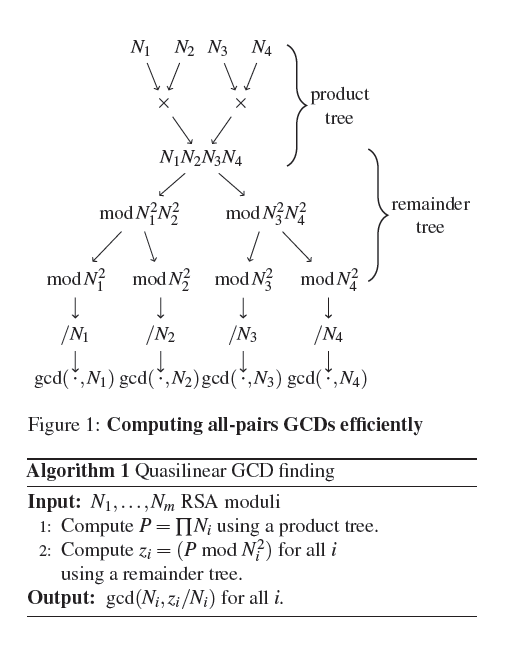
\includegraphics[scale=0.7]{figures/Bernstein_Computing-all-pairs-GCDs.png}
\caption{Algorithmus und Abbildung, um alle ggTs effizient zu berechnen}
\label{Figure_Bernstein_Computing-all-pairs-GCDs}
\end{center}
\end{figure}


Der Artikel~\cite{Heninger2012} erklärt sehr gut \textit{wie} der Algorithmus funktioniert, aber nicht so gut \textit{warum}. Das Produkt $P$ aller Module ist eine sehr große Zahl, sogar wenn man sie mit den einzelnen Modulen vergleicht. Ohne die Vereinfachungen durch den Restebaum würde man folgendermaßen vorgehen: Berechnen von $ggT_{i} = ggT( P / m_{i},  m_{i}) $ für alle $i$. Vergleichen jedes $ggT_{i} \ne 1$ mit allen anderen $ggT_{j} \ne 1$ mit  $j \ne i$. Wenn zwei ggTs gleich sind, haben ihre Module einen gemeinsamen Faktor.\footnote{%
Eine Voraussetzung dafür, dass man nur Primfaktoren erhält, ist, dass doppelte Module entfernt werden, bevor man den Baum aufsetzt.
}

Weil diese Berechnungen bei den großen Längenunterschieden der Zahlen sehr langsam sind, wird der Restebaum benutzt. Obwohl es so aussieht, als benötige er mehr Schritte, bedeutet er eine große Vereinfachung.

Innerhalb des Restebaums erhält man -- am Ende -- $(P \bmod ({m_{i}^{2}}) ) / m_{i}$ für alle $i$.\footnote{%
Es würde keinen Sinn machen, beim linken ggT modulo $m_{i}$ statt $m_{i}^{2}$
zu rechnen, denn das bedeutete, $(P \bmod m_{i} ) / m_{i}$ zu benutzen: Denn
$m_{i} | P$, so dass $P/m_{i}$ immer eine ganze Zahl ist, so dass
$(P \bmod m_{i} )$ immer $= 0$ ist.

\noindent Beispiel mit sehr kleinen Modulen:\\
$ m_{1} = 2*3 = 6;~~~ m_{2} = 2*7 = 14;~~~ P=6*14=84 $\\
$ P \bmod m_{1} = 84 \bmod 6 = 0;~~~ P \bmod {m_{1}^{2}} = 84 \bmod 36 = 12 $\\
$ P \bmod m_{2} = 84 \bmod 14 = 0;~~~ P \bmod {m_{2}^{2}} = 84 \bmod 196 = 84 $\\
$ggT_{1} = ggT(12/6, 6) = ggT(2, 6) = 2 $\\
$ggT_{2} = ggT(84/14, 14) = ggT(6, 14) = 2 $

So wie der Baum strukturiert ist, würde es auch keinen Sinn machen, zuerst zu
teilen und dann die Modulo-Operation vorzunehmen, denn das würde zu den gegebenen Modulen in umgekehrter Reihenfolge führen.

Ebenfalls keinen Sinn würde es machen, $(P \bmod ({m_{i}^{3}}) ) / {m_{i}^{2}})$ zu berechnen, da dies nur zusätzlichen Aufwand ohne Verbesserung bedeutet.
}

Die wesentliche offene Frage ist noch: Warum liefert $ggT((P \bmod {m_{i}^{2}})/ m_{i}, m_{i})$ dasselbe Ergebnis wie $ggT( P / m_{i}, m_{i})$?
Wir beweisen, dass diese Identität korrekt ist.\footnote{%
P ist das Produkt aller Module, und $m_{i}$ ist irgendein Modul.
}

$$ggT((P \bmod {m_{i}^{2}})/ m_{i}, m_{i})~~~  \overset{!}{=}  ~~~ggT( P / m_{i}, m_{i})$$
$ \Longleftrightarrow $~~~\footnote{Gemäß Euklids Algorithmus (erste Iteration) ist die folgende Identität wahr:\\
$ggT(a, b) = ggT(b, a \bmod b)$ wenn $ b \neq 0 $\\
Dies gilt, weil per Definition gilt: $ggT(a, 0) = a$\\
Angewandt auf unsere Problem bedeutet das:
\mbox{}\\
$ggT((P \bmod {m_{i}^{2}})/ m_{i}, m_{i})=ggT((P \bmod {m_{i}^{2}})/ m_{i} \bmod{m_{i}}, m_{i})$ \mbox{}\\
$ggT( P / m_{i}, m_{i})=ggT( P / m_{i} \bmod{m_{i}}, m_{i})$\mbox{}
}

$$ggT(((P \bmod {m_{i}^{2}})/ m_{i}) \bmod {m_{i}}, m_{i})~~~  \overset{!}{=}  ~~~ggT( (P / m_{i}) \bmod {m_{i}}, m_{i})$$
$ \Longleftrightarrow $~~~\footnote{Die ggTs sind gleich, wenn ihre beiden ersten Argumente gleich sind.
}

$$((P \bmod {m_{i}^{2}})/ m_{i}) \bmod {m_{i}}~~~  \overset{!}{=}  ~~~ (P / m_{i}) \bmod {m_{i}}$$
$ \Longleftrightarrow $~~~\footnote{Die folgenden Umformungen sind Äquivalenzumformungen.
}

$$(P \bmod{m_{i}^{2}})/ m_{i} - P / m_{i} \equiv 0   \bmod{m_{i}}~~~ \Leftrightarrow ~~~  m_{i} ~~ | ~~ ((P \bmod{m_{i}^{2}})/ m_{i} - P / m_{i})$$~~~\footnote{%
Benutzt man die Modulo-Operation (Definition \ref{def-zth-remainder} von Seite
\pageref{def-zth-remainder}) und eine Division, ergibt sich:
$~a \bmod{b} ~ =  ~ a - b * \lfloor a/b \rfloor$. So kann $P \bmod{m_{i}^{2}}$ geschrieben werden als $ P-m_{i}^{2} \lfloor P/m_{i}^{2} \rfloor$.
}

$$ m_{i} ~~ | ~~ ((P-m_{i}^{2}* \lfloor P/m_{i}^{2} \rfloor - P))/m_{i}$$~~~\footnote{%
$P$ reduziert sich selbst, der Exponent von $m_{i}$ im Zähler kürzt sich mit dem $m_{i}$ im Nenner.
}

$$ m_{i} ~~ | ~~ (m_{i}* \lfloor P/m_{i}^{2} \rfloor)$$

Weil dies offensichtlich wahr ist, können wir schließen, dass die zwei ggTs äquivalent sind.

% yyyyyyyyyyyyyyyyyyyyyyyyyyy
% Sätze und Links:
% https://en.wikipedia.org/wiki/Greatest_common_divisor
% https://de.wikipedia.org/wiki/Gr%C3%B6%C3%9Fter_gemeinsamer_Teiler



% ++++++++++++++++++++++++++++++++++++++++++++++++++++++++++++++++++++++++++
\newpage
\begin{ctsquote}
Viel mehr als unsere Fähigkeiten sind es
unsere Entscheidungen \dots, die zeigen, wer wir wirklich sind.
\caption[Joanne K. Rowling]{Joanne K. Rowling\footnotemark}\index{Rowling, Joanne}
\end{ctsquote}

\addtocounter{footnote}{0}\footnotetext{Joanne K. Rowling,
\glqq Harry Potter und die Kammer des Schreckens\grqq, Carlsen, 1998,
letztes Kapitel \glqq Dobbys Belohnung\grqq, S.~343, Dumbledore.}

% ++++++++++++++++++++++++++++++++++++++++++++++++++++++++++++++++++++++++++
\section{Anwendungen asymmetrischer Kryptographie mit Zahlenbeispielen}

In der modernen Kryptographie \index{Kryptographie!modern} werden die Ergebnisse
der modularen Arithmetik extensiv angewandt. Hier werden exemplarisch einige
wenige Beispiele aus der Kryptographie mit kleinen\footnote{%
\glqq Klein\grqq~bedeutet beim RSA-Verfahren, dass die Bitlängen der Zahlen sehr
viel kleiner sind als $1024$ Bit (das sind $308$ Dezimalstellen).
$1024$ Bit gilt im Moment in der Praxis als Mindestlänge für sichere RSA-Module.
} Zahlen vorgestellt.\footnote{%
Didaktisch sehr gut aufbereitete Artikel mit Programmbeispielen in Python\index{Python}
und SageMath finden sich in der Artikelserie {\em RSA \& Co. in der Schule:
Moderne Kryptologie, alte Mathematik, raffinierte Protokolle}.
Siehe beispielsweise \cite{Witten2015}.\index{RSA \& Co. in der Schule}
}

Die Chiffrierung eines Textes besteht darin, dass man aus einer Zeichenkette
(Zahl) durch Anwenden einer Funktion (mathematische Operationen) eine andere
Zahl erzeugt. Dechiffrieren heißt, diese Funktion umzukehren: aus dem
Zerrbild, das die Funktion aus dem Klartext gemacht hat, das Urbild
wiederherzustellen. Beispielsweise könnte der Absender einer vertraulichen
Nachricht zum Klartext $M$ eine geheimzuhaltende Zahl, den Schlüssel $S$,
addieren und dadurch den Chiffretext $C$ erhalten:
$$ C = M + S. $$
Durch Umkehren dieser Operation, das heißt durch Subtrahieren von $S$, kann
der Empfänger den Klartext rekonstruieren:
$$ M = C - S. $$
Das Addieren von $S$ macht den Klartext zuverlässig unkenntlich. Gleichwohl
ist diese Verschlüsselung sehr schwach; denn wenn ein Abhörer auch nur ein
zusammengehöriges Paar von Klar- und Chiffretext in die Hände bekommt, kann
er den Schlüssel berechnen
$$ S = C - M, $$
und alle folgenden mit $S$ verschlüsselten Nachrichten mitlesen.\\
Der wesentliche Grund ist, dass Subtrahieren eine ebenso einfache Operation
ist wie Addieren.



% --------------------------------------------------------------------------
\hypertarget{OneWayFunktion2}{}%
\subsection{Einwegfunktionen}\index{Einwegfunktion}
\label{OneWayFunktion2}%
Wenn der Schlüssel auch bei gleichzeitiger Kenntnis von
Klar- und Chiffretext nicht ermittelbar sein soll, braucht man eine
Funktion, die einerseits relativ einfach berechenbar ist - man will ja
chiffrieren können. Andererseits soll ihre Umkehrung zwar existieren (sonst
würde beim Chiffrieren Information verlorengehen), aber de facto
unberechenbar sein.

Was sind denkbare Kandidaten für eine solche \textbf{Einwegfunktion}?
Man könnte an
die Stelle der Addition die Multiplikation setzen; aber schon Grundschüler
wissen, dass deren Umkehrung, die Division, nur geringfügig mühsamer ist als
die Multiplikation selbst. Man muss noch eine Stufe höher in der Hierarchie
der Rechenarten gehen: Potenzieren ist immer noch eine relativ einfache
Operation; aber ihre beiden Umkehrungen {\em Wurzelziehen} (finde $b$ in der
Gleichung $a = b^c$ , wenn $a$ und $c$ bekannt sind) und {\em Logarithmieren} (in
derselben Gleichung finde $c$, wenn $a$ und $b$ bekannt sind) sind so kompliziert,
dass ihre Ausführung in der Schule normalerweise nicht mehr gelehrt wird.

Während bei Addition und Multiplikation noch eine gewisse Struktur
wiedererkennbar ist, wirbeln Potenzierung und Exponentiation alle Zahlen
wild durcheinander: Wenn man einige wenige Funktionswerte kennt, weiß man
(anders als bei Addition und Multiplikation) noch kaum etwas über die
Funktion im ganzen.



% --------------------------------------------------------------------------
\vskip +10 pt
\subsection{Das Diffie-Hellman Schlüsselaustausch-Protokoll}
\index{Diffie, Whitfield}
\index{Hellman, Martin}
\index{Diffie-Hellman}

Das DH-Schlüsselaustauschprotokoll (Key Exchange Protocol) wurde 1976 in
Stanford von Whitfield Diffie, Martin E. Hellman und Ralph Merkle erdacht.\footnote{%
  In CT1\index{CT1} ist dieses Austauschprotokoll visualisiert:
  Sie können die einzelnen Schritte mit konkreten Zahlen nachvollziehen
  per Menü \textbf{Einzelverfahren \textbackslash{} Protokolle
           \textbackslash{} Diffie-Hellman-Demo}.\\
  In JCT\index{JCT} findet man es in der Standard-Perspektive
  über den Menüeintrag \textbf{Visualisierungen \textbackslash{} Diffie-Hellman
  Schlüsselaustausch (EC)}.
}

Eine Einwegfunktion dient Alice und Bob\footnote{%
Alice\index{Alice} und Bob\index{Bob} werden standardmäßig als die beiden
berechtigten Teilnehmer eines Protokolls bezeichnet (siehe
\cite[Seite 23]{Schneier1996}).
} dazu, sich einen Schlüssel $S$, den Sessionkey, für die nachfolgende
Verständigung zu verschaffen. Dieser ist dann ein Geheimnis, das nur diesen
beiden bekannt ist. Alice wählt sich eine Zufallszahl $a$ und hält sie geheim.
Aus $a$ berechnet sie mit der Einwegfunktion die Zahl $A = g^a$ und schickt sie
an Bob. Der verfährt ebenso, indem er eine geheime Zufallszahl $b$ wählt,
daraus $B = g^b$ berechnet und an Alice schickt. Die Zahl $g$ ist beliebig und
darf öffentlich bekannt sein. Alice wendet die Einwegfunktion mit ihrer
Geheimzahl $a$ auf $B$ an, Bob tut gleiches mit seiner Geheimzahl $b$ und der
empfangenen Zahl $A$.

Das Ergebnis $S$ ist in beiden Fällen dasselbe, weil die Einwegfunktion
kommutativ ist: $g^{a*b} = g^{b*a}$. Aber selbst Bob kann Alices Geheimnis $a$ nicht aus
den ihm vorliegenden Daten rekonstruieren, Alice wiederum Bobs Geheimnis $b$
nicht ermitteln, und ein Lauscher, der $g$ kennt und sowohl $A$ als auch $B$
mitgelesen hat, vermag daraus weder $a$ noch $b$ noch $S$ zu berechnen.

\vskip +10 pt
\input{figures/DH-de.latex}
\vskip +20 pt

\noindent \textbf{Ablauf:}\par
\nopagebreak
\noindent Alice und Bob wollen also einen geheimen Sessionkey $S$ über einen
abhörbaren Kanal aushandeln.
\begin{itemize}
   \item[\textbf{1.}] Sie wählen eine Primzahl $p$ und eine Zufallszahl $g$, und tauschen diese
                 Information offen aus.
   \item[\textbf{2.}] Alice wählt nun $a$, eine Zufallszahl kleiner $p$ und
                 hält diese geheim.

                 Bob wählt ebenso $b$, eine Zufallszahl kleiner $p$ und
                 hält diese geheim.
   \item[\textbf{3.}] Alice berechnet nun $A \equiv g^a {\rm ~(mod~} p)$.\\
                 Bob berechnet $B \equiv g^b {\rm ~(mod~} p)$.
   \item[\textbf{4.}] Alice sendet das Ergebnis $A$ an Bob.\\
                 Bob sendet das Ergebnis $B$ an Alice.
   \item[\textbf{5.}] Um den nun gemeinsam zu benutzenden Sessionkey zu bestimmen,
                 potenzieren sie beide jeweils für sich das jeweils empfangene
                 Ergebnis mit ihrer geheimen Zufallszahl modulo $p$. Das heißt:
         \begin{itemize}
                    \item[-] Alice berechnet $S \equiv B^a {\rm ~(mod~} p)$, und
                    \item[-] Bob berechnet   $S \equiv A^b {\rm ~(mod~} p)$.
         \end{itemize}
\end{itemize}
Auch wenn ein Spion $g, p$, und die Zwischenergebnisse $A$ und $B$ abhört, kann
er den schließlich bestimmten Sessionkey nicht berechnen -- wegen der
Schwierigkeit, den diskreten Logarithmus\footnotemark~zu bestimmen.
\footnotetext{%
Weitere Details zum \index{Logarithmusproblem!diskret}
\hyperlink{HT-Discrete-Logarithm-as-Basis}{Diskreten Logarithmusproblem}
finden Sie in den Kapiteln~\ref{L-Discrete-Logarithm-as-Basis} und \ref{Chapter_Dlog-FactoringDead}.
}

\vskip +10 pt
\noindent Das Ganze soll an einem Beispiel mit (unrealistisch) kleinen Zahlen gezeigt
werden.\vskip +1em

\begin{example}{ mit kleinen Zahlen:}
\begin{itemize}
   \item[\textbf{1.}] Alice und Bob wählen $g = 11$, $p = 347$.
   \item[\textbf{2.}] Alice wählt $a = 240$, Bob wählt $b = 39$ und behalten $a$ und $b$ geheim.
   \item[\textbf{3.}] Alice berechnet $A \equiv g^a \equiv 11^{240} \equiv 49 {\rm ~(mod~} 347).$\\
                 Bob berechnet $B \equiv g^b \equiv 11^{39} \equiv 285 {\rm ~(mod~} 347).$
   \item[\textbf{4.}] Alice sendet Bob: $A = 49$,\\
                 Bob sendet Alice: $B = 285$.
   \item[\textbf{5.}] Alice berechnet $B^a \equiv 285^{240} \equiv 268 {\rm ~(mod~}347),$\\
                 Bob berechnet $A^b \equiv 49^{39} \equiv 268 {\rm ~(mod~}347)$.
\end{itemize}
Nun können Alice und Bob mit Hilfe ihres gemeinsamen Sessionkeys $S$ sicher
kommunizieren. Auch wenn ein Spion alles abhörte, was über die Leitung ging:
$g = 11, p = 347, A = 49$ und $B = 285$; den geheimen Schlüssel $S$ kann er nicht
berechnen.

\noindent Dies ist aber nur für sehr große Zahlen so, weil der diskrete Logarithmus
nur dann extrem schwierig gefunden werden kann (siehe Kapitel \ref{Chapter_Dlog-FactoringDead}).

\end{example}


\newpage
\begin{remark}{:}

\noindent Für solch kleine Zahlen wie in dem obigen Beispiel ist das
DH-Schlüsselaustausch-Protokoll angreifbar, da das diskrete
Logarithmusproblem\index{Logarithmusproblem!diskret} leicht berechnet
werden kann, um die Exponenten $a$ oder $b$ zu finden.

\noindent Wenn man $a$ oder $b$ hat, kann man $S$ genauso berechnen
wie es Alice or Bob vorher machten.

\noindent Um die diskreten Logarithen\index{Logarithmusproblem!diskret}
zu erhalten, ist hier Folgendes zu berechnen:

$a$ von Alice: $11 ^ x \equiv 49 \pmod{347}$, also $\log_{11}(49) \pmod{347}$.

$b$ von Bob:   $11 ^ y \equiv 285 {\rm ~(mod~}347)$, also $\log_{11}(285){\rm ~(mod~}347)$.


\noindent Mit SageMath\index{SageMath} kann man den diskreten Logarithmus $x$,
der die obige Gleichung (z.B. für Allice) löst:

\begin{sagecode}
\begin{Verbatim}%
[fontsize=\footnotesize]
# Get the secret key of Alice:
### via numbers
sage: discrete_log(mod(49,347),mod(11,347))
67
### via variables in the ring of integers
sage: R=Integers(347)
sage: g=R(11)
sage: A=R(49)
sage: discrete_log(A,g)
67

# Get the secret key of Bob:
sage: B=R(285)
sage: discrete_log(B,g)
39
\end{Verbatim}
\caption{Beispiel mit kleinen Zahlen: Berechnen der diskreten Logs $a$ und $b$, um DH anzugreifen}
\end{sagecode}

\noindent Da die SageMath-Funktion discrete\_log als Argumente nur
Elemente eines Rings erwartet (Integer zwischen 0 und einer Obergrenze),
können wir diesen Typ einerseits erzwingen, indem wir die Zahlen direkt mit dem
zugehörigen Modulo-Operator eingeben: \texttt{discrete\_log(mod(49, 347), mod(11, 347))}.\\
Eine viel bessere Alternative ist es, die Variablen so wie in der obigen Formel
zu benutzen und SageMath wissen zu lassen, dass es sich um Elements eines Rings handelt.
Nach diesem \glqq Mehraufwand\grqq~zu Beginn für die Initialisierung, kann man die Formeln
genauso niederschreiben, wie man es gewohnt ist: \texttt{discrete\_log(A, g)}.\footnote{%
Solche zahlentheoretischen Aufgaben können auch mit anderen Tools wie PariGP\index{Pari-GP},
LiDIA\index{LiDIA}, BC\index{BC} oder Mathematica\index{Mathematica}
(siehe Anhang Web-Links am Ende dieses Kapitel) gelöst werden:
Hier die entsprechende Syntax, um den diskreten Log für Alice zu bekommen:
	\begin{compactitem}
	\item Pari-GP: \texttt{znlog(Mod(49,347),Mod(11,347))}
	\item LiDIA:   \texttt{dl(11,49,347)}
	\item Mathematica: {\tt MultiplicativeOrder[11, 347, 49]}\\
		Die allgemeine Funktion \glqq Solve\grqq~liefert die  \glqq {em tdep message}\grqq:
		The equations appear to involve the variables to be solved
		for in an essentially non-algebraic way.
	\end{compactitem}
Alle liefern das Ergebnis $67$.
}${}^,$\footnote{%
Warum haben die Funktionen für den diskreten
Logarithmus\index{DL-Problem}\index{Logarithmusproblem!diskret}\index{diskreter Logarithmus} für Alice
den Wert $67$ geliefert und nicht den Wert 240, den Alice als Exponent $a$ wählte?\\
Der diskrete Logarithmus ist der kleinste natürliche Exponent, der die
Gleichung $11^x \equiv 49{\rm ~(mod~}347)$ löst. Sowohl $x=67$ als auch $x=240$ (die im Beispiel
gewählte Zahl) erfüllen die Gleichung und können damit zur Berechnung des
Sessionkeys benutzt werden: $285^{240}  \equiv 285^{67} \equiv 268 {\rm ~(mod~}347)$.
Hätten Alice und Bob als Basis $g$ eine Primitivwurzel\index{Primitivwurzel} modulo $p$ gewählt,
dann gibt es für jeden Rest aus der Menge
$\{1, 2, \cdots, p-1\}$ genau einen Exponenten aus der Menge $\{0, 1, \cdots, p-2\}.$\\
\indent Info: Zum Modul $347$ gibt es $172$ verschiedene Primitivwurzeln, davon sind $32$
prim (ist nicht notwendig).
Da die im Beispiel für $g$ gewählte Zahl $11$ keine Primitivwurzel\index{Primitivwurzel}
von $347$ ist, nehmen die Reste nicht alle Werte aus der Menge $\{1, 2, \cdots, 346\}$ an.
Somit kann es für einen bestimmten Rest mehr als einen oder auch gar keinen
Exponenten aus der Menge $\{0, 1, \cdots, 345\}$ geben, der die Gleichung
erfüllt.\\
Mit den entsprechenden SageMath-Funktionen\index{SageMath} findet man:\\
\texttt{is\_prime(347)=True}, \texttt{euler\_phi(347)=346}, \texttt{gcd(11,347)=1} und
\texttt{multiplicative\_order(mod(11, 347))=173}.

\begin{tabular}{|c|c|l|}
\hline
i  & $11^i \bmod 347$ &\\
\hline
      0  &          1   &\\
      1  &         11   &\\
      2  &        121   &\\
      3  &        290   &\\
     67  &         49   & gesuchter Exponent\\
    172  &        284   &\\
    173  &          1   &= Multiplikative Ordnung von $11^i ~(\bmod 347)$\\
    174  &         11   &\\
    175  &        121   &\\
    176  &        290   &\\
    240  &         49   & gesuchter Exponent\\
\hline
\end{tabular}
\vskip +6 pt

\noindent Weitere Details finden Sie~
in Kapitel~\ref{nt:AppArith3a2} \glqq \nameref{nt:AppArith3a2}\grqq.
}

\end{remark}



% ++++++++++++++++++++++++++++++++++++++++++++++++++++++++++++++++++++++++++
\newpage
\hypertarget{RSAKonkret}{}%
\hypertarget{Chapter_ElementaryNT_12}{}%ist wahrscheinlich redundant !
\section[Das RSA-Verfahren mit konkreten Zahlen]
	{Das RSA-Verfahren mit konkreten Zahlen\footnotemark}
\footnotetext{%
    \index{SageMath}%
    \index{Nguyen, Minh Van }%
    Nguyen schrieb einen kurzen und didaktisch sehr klaren Artikel zu einigen
    Grundlagen der Zahlentheorie und zur Benutzung von SageMath \cite{Nguyen2009a}.
}
\label{rsaconcrete}\index{RSA}

\begin{ctsquote}
\glqq Das Spiel ist eine Erfindung der Natur, um uns auf schwierige Realitäten vorzubereiten. Sind Sie jetzt endlich bereit, der Realität ins Auge zu sehen, Sergeant?\grqq
\caption[Daniel Suarez]{Daniel Suarez\footnotemark}\index{Suarez, Daniel}
%Der erste String nach \caption geht in das Zitate-Verzeichnis.
\end{ctsquote}
\addtocounter{footnote}{0}\footnotetext{Daniel Suarez, \glqq Daemon\grqq, rororo, (c) 2010,
Kapitel 45, \glqq Wiedereintritt\grqq, S. 615, Sobol.}

Nachdem oben die \hyperlink{RSA}{Funktionsweise des RSA-Verfahrens} beschrieben
wurde, sollen diese Schritte hier mit konkreten, aber kleinen Zahlen
durchgeführt werden.


% --------------------------------------------------------------------------
\subsection{RSA mit kleinen Primzahlen und mit einer Zahl als Nachricht}
Bevor wir RSA auf einen Text anwenden, wollen wir es erst direkt mit einer
Zahl\footnote{%
   In der Praxis wird RSA nie auf Texte angewandt, sondern nur auf große Zahlen.
}
zeigen.\footnote{%
   Mit CT1\index{CT1} können Sie dies per Menü \textbf{Einzelverfahren
   \textbackslash{} RSA-Kryptosystem \textbackslash{} RSA-Demo} lösen.
}
\begin{itemize}
  \item[\textbf{1.}] Die gewählten Primzahlen seien $p=5$ und $q=11$.\\
                Also ist $n=55$ und $\phi(n) = (p-1)*(q-1)=40$.
  \item[\textbf{2.}] $e = 7$ ($e$ sollte\footnote{%
                Siehe Fußnote~\ref{foot:Selection-of-e} auf Seite
                \pageref{foot:Selection-of-e}.} zwischen $11$ und $39$ liegen,
                und muss teilerfremd\index{Zahlen!teilerfremd (co-prime)}
                zu $40$ sein).
  \item[\textbf{3.}] $d = 23$ (da $23*7 \equiv 161 \equiv 1{\rm ~(mod~}40)$)
  \begin{itemize}
     \item[] $\rightarrow$ Public-Key des Empfängers: $(55, 7),$
     \item[] $\rightarrow$ Private-Key des Empfängers: $(55, 23).$
  \end{itemize}
  \item[\textbf{4.}] Nachricht sei nur die Zahl $M = 2$ (also ist kein
                Aufbrechen in Blöcke nötig).
  \item[\textbf{5.}] Verschlüsseln: $C \equiv 2^7 \equiv 18 {\rm ~(mod~}55).$
  \item[\textbf{6.}] Chiffrat ist nur die Zahl $C = 18$ (also kein Aufbrechen
                in Blöcke nötig).
  \item[\textbf{7.}] Entschlüsseln: $M \equiv 18^{23} \equiv 18^{(1+2+4+16)} \equiv 18*49*36*26 \equiv 2 {\rm ~(mod~}55).$
\end{itemize}
Nun wollen wir RSA auf einen Text anwenden: zuerst mit dem
Großbuchstabenalphabet (26 Zeichen), dann mit dem gesamten
ASCII-Zeichensatz als Bausteine für die Nachrichten.


% --------------------------------------------------------------------------
\subsection{RSA mit etwas größeren Primzahlen und einem Text aus Großbuchstaben}\label{rsaex2}
Gegeben ist der Text \glqq ATTACK AT DAWN\grqq, und die Zeichen werden gemäß
Tabelle~\ref{alphacode}\index{Blocklänge} codiert.\footnote{%
Mit CT1\index{CT1} können Sie dies per Menü
\textbf{Einzelverfahren \textbackslash{} RSA-Kryptosystem \textbackslash{} RSA-Demo} lösen.
Dies ist auch im Tutorial/Szenario der Online-Hilfe zu CT1 beschrieben [Optionen,
Alphabet vorgeben, Basissystem, Blocklänge\index{Blocklänge} 2 und Dezimaldarstellung].
}

\begin{table}[ht]
\begin{center}
\begin{tabular}{|c|l||c|l|}
\hline
Zeichen & Zahlenwert & Zeichen & Zahlenwert\\
\hline
\hline
Blank    & 0   & M    & 13\\
A        & 1   & N    & 14\\
B        & 2   & O    & 15\\
C        & 3   & P    & 16\\
D        & 4   & Q    & 17\\
E        & 5   & R    & 18\\
F        & 6   & S    & 19\\
G        & 7   & T    & 20\\
H        & 8   & U    & 21\\
I        & 9   & V    & 22\\
J       & 10   & W    & 23\\
K       & 11   & X    & 24\\
L       & 12   & Y    & 25\\
&              & Z    & 26\\
\hline
\end{tabular}
\end{center}
\hypertarget{Grossbuchstaben-Alphabet}{}
\caption{Großbuchstabenalphabet}\index{Großbuchstabenalphabet}
\label{alphacode}
\end{table}

\noindent \textbf{Schlüsselerzeugung (Schritt 1 bis 3):}\\
%\vskip 5 pt
\textbf{1.} $p=47, q=79$ $( n= 3713;~ \phi(n) = (p-1)*(q-1)=3588).$\\
\textbf{2.} $e=37$ ($e$ sollte\footnote{%
                Siehe Fußnote~\ref{foot:Selection-of-e} auf Seite
                \pageref{foot:Selection-of-e}.}  zwischen 79 und 3587 liegen,
                und muss teilerfremd\index{Zahlen!teilerfremd (co-prime)}
                zu $3588$ sein).\\
\textbf{3.} $d=97$ (denn $e*d=1{\rm ~mod~}\phi(n); 37*97 \equiv 3589
\equiv 1{\rm ~(mod~}3588) \;$).\footnote{%
  Wie man $d = 97$ mit Hilfe des erweiterten ggT berechnet, wird in
  Anhang~\ref{nt:NumberTheory_Appendix_GCD} gezeigt.
}

\noindent \textbf{4. Verschlüsselung:}\\
{\tt
\begin{tabular}{rcccccccccccccccccccc}
{\rm Text:} & A & T & T & A & C & K & & A & T &  & D & A & W & N\\
{\rm Zahl:} & 01 & 20 & 20 & 01 & 03 & 11 & 00 & 01 & 20 & 00 & 04 & 01 & 23 & 14
\end{tabular}
}
\index{Blocklänge}

\noindent Aufteilung dieser 28-stelligen Zahl in 4-stellige Teile (denn $2626$ ist noch kleiner als $n=3713$), d.h. dass
die Blocklänge 2 beträgt.\\
{\tt 0120 2001 0311 0001 2000 0401 2314}

\label{SrcArith4a}
\noindent Verschlüsselung aller 7 Teile jeweils per: $C \equiv M^{37}{\rm ~(mod~3713)}$:\footnote{%
  In Kapitel~\ref{nt:AppArith4a} \glqq \nameref{nt:AppArith4a}\grqq~
  finden Sie den Beispiel-Quelltext zur RSA-Verschlüsselung mit SageMath.
}\\
{\tt 1404 2932 3536 0001 3284 2280 2235}

\noindent \textbf{5. Entschlüsselung:}\\
Chiffrat: {\tt 1404 2932 3536 0001 3284 2280 2235 }

\noindent Aufteilung dieser 28-stelligen Zahl in 4-stellige Teile.

\noindent Entschlüsselung aller $7$ Teile jeweils per: $M \equiv C^{97}{\rm ~(mod~}3713)$:\\
{\tt 0120 2001 0311 0001 2000 0401 2314}

\noindent Umwandeln von 2-stelligen Zahlen in Großbuchstaben und Blanks.

\noindent Bei den gewählten Werten ist es für einen Kryptoanalytiker
\index{Kryptoanalyse} einfach, aus den öffentlichen Parametern
$n=3713$ und $e=37$ die geheimen Werte zu finden, indem
er offenlegt, dass $3713 = 47 * 79$.

\noindent Wenn $n$ eine $1024$-Bit-Zahl ist, bestehen dafür -- nach heutigen
Kenntnissen -- wenig Chancen.


% --------------------------------------------------------------------------
\subsection[RSA mit noch etwas größeren Primzahlen und ASCII-Zeichen]
           {RSA mit noch etwas größeren Primzahlen und mit einem Text aus ASCII-Zeichen}

Real wird das ASCII-Alphabet benutzt, um die Einzelzeichen der Nachricht in
8-Bit lange Zahlen zu codieren.

\noindent Diese Aufgabe\footnote{%
Mit CT1\index{CT1} können Sie diese Aufgabe per Menü
  \textbf{Einzelverfahren \textbackslash{} RSA-Kryptosystem \textbackslash{}
  RSA-Demo} lösen.\\
  Mit JCT\index{JCT} können Sie diese Aufgabe im Menü
  \textbf{Visualisierungen \textbackslash{} RSA-Kryptosystem}
  der Standard-Perspektive lösen.%xxxxxxxxxxxxxxxxTODOxxxxxxxxxxxxxxxxxxxxCT2?
}
ist angeregt durch das Beispiel aus \cite[S. 271]{Eckert2014}.
% Eigentlich stammte die Aufgabe aus Eckert2001, S. 215. Diese 1. Buchausgabe
% ist nun nicht mehr im Literaturverzeichnis (6.6.2, Das RSA-Verfahren,
% Bsp. 6.14 (ASCII-Codierung).
% In Eckert2001 passten nur die Zahlen nicht ganz, so dass ich andere
% wählte bei gl. Text. In Eckert 20003 sind nochmal andere Zahlen,
% aber ich ließ das Skript unverändert.

\noindent Der Text \glqq RSA works!\grqq~bedeutet in Dezimalschreibweise codiert:

{\tt
\begin{tabular}{rcccccccccccccccccccc}
{\rm Text:} & R & S & A &   & w & o & r & k & s & !\\
{\rm Zahl:} & 82 & 83 & 65 & 32 & 119 & 111 & 114 & 107 & 115 & 33
\end{tabular} } % \tt

\noindent Das Beispiel wird in 2 Varianten durchgespielt. Gemeinsam für beide sind die Schritte $1$ bis $3$.
\vskip +10pt
\noindent \textbf{Schlüsselerzeugung (Schritt 1 bis 3):}\\\label{SrcArith4b}%
\textbf{1.} $p=509,~q=503 \quad (n= 256.027; \; ~\phi(n)=(p-1)*(q-1)=255.016=2^3*127*251)$.\footnote{%
  In Kapitel~\ref{nt:AppArith4b} \glqq \nameref{nt:AppArith4b}\grqq~
  finden Sie den Quelltext zur Faktorisierung von $\phi(n)$ mit SageMath.
}\\
\textbf{2.} $e=65.537$ ($e$ sollte\footnote{%
                Siehe Fußnote~\ref{foot:Selection-of-e} auf Seite
                \pageref{foot:Selection-of-e}.}
                zwischen $509$ und $255.015$ liegen, u. muss\footnote{%
                $e$ darf also nicht $2, 127$ oder $251$ sein
                ($65537 = 2^{16}+1$) ($255,016 = 2^{3}*127*251$).\\
                Real wird $\phi(n)$ nicht faktorisiert, sondern für das gewählte
                $e$ wird mit dem Euklidschen Algorithmus sichergestellt, dass
                ggT$(e,\phi(n))=1$.
                }
      teilerfremd\index{Zahlen!teilerfremd (co-prime)} zu $255.016$ sein).\\
\textbf{3.} $d=231.953$\\
\strut\quad\ (denn $e \equiv d^{-1}{\rm ~mod~}\phi(n);$
\mbox{}\quad $65.537*231.953 \equiv 15.201.503.761 \equiv 1
{\rm ~(mod~}255.016))$.\footnote{%
Andere mögliche Kombinationen von (e,d) sind z.B.: (3, 170.011), (5, 204.013), (7, 36.431).
}


% --------------------------------------------------------------------------
\subsection*{Variante 1:\\ ASCII-Zeichen werden einzeln ver- und entschlüsselt (keine Blockbildung).}

\textbf{4. Verschlüsselung:}\\
{\tt
\begin{tabular}{rcccccccccccccccccccc}
{\rm Text:} & R & S & A &   & w & o & r & k & s & !\\
{\rm Zahl:} & 82 & 83 & 65 & 32 & 119 & 111 & 114 & 107 & 115 & 33
\end{tabular} } % \tt

\noindent Keine Zusammenfassung der Buchstaben!\footnote{%
Für sichere Verfahren braucht man große Zahlen, die möglichst alle Werte bis
$n-1$ annehmen. Wenn die mögliche Wertemenge der Zahlen in der Nachricht zu
klein ist, nutzen auch große Primzahlen nichts für die Sicherheit.
Ein ASCII-Zeichen ist durch $8$ Bits repräsentiert. Will man größere Werte,
muss man mehrere Zeichen zusammenfassen. Zwei Zeichen benötigen 16 Bit, womit
maximal der Wert 65.536 darstellbar ist; dann muss der Modul $n$ größer sein als
$2^{16} = 65.536$. Dies wird in Variante 2 angewandt.
Beim Zusammenfassen bleiben in der Binär-Schreibweise die führenden Nullen
erhalten (genauso wie wenn man oben in der Dezimalschreibweise alle Zahlen
3-stellig schreiben würde und dann die Folge {\tt 082 083, 065 032,
119 111, 114 107, 115 033} hätte).
}
\label{SrcArith4c}\\
Verschlüsselung pro Zeichen per: $C \equiv M^{65.537}{\rm ~(mod~}256.027)$:\footnote{%
%%  In Kapitel~\ref{nt:AppArith4c} \glqq \nameref{nt:AppArith4c}\grqq~
%%  finden Sie den Quelltext zur RSA-Exponentiation mit SageMath.  %%% BE_War gerade so lange, dass danach eine Leerzeile.
  Kapitel~\ref{nt:AppArith4c} \glqq \nameref{nt:AppArith4c}\grqq~
  enthält den Quelltext zur RSA-Exponentiation mit SageMath.
}\\
{\tt
\begin{tabular}{lllll}
212984 & 025546 & 104529 & 031692 & 248407\\
100412 & 054196 & 100184 & 058179 & 227433\\
\end{tabular}
}

\noindent \textbf{5. Entschlüsselung:}\\
Chiffrat:\\
{\tt
\begin{tabular}{lllll}
212984 & 025546 & 104529 & 031692 & 248407\\
100412 & 054196 & 100184 & 058179 & 227433\\
\end{tabular} }

\noindent Entschlüsselung pro Zeichen per: $M \equiv C^{231.953}{\rm ~mod~}256.027$:\\
{\tt 82 83 65 32 119 111 114 107 115 33}\\


% --------------------------------------------------------------------------
\subsection*{Variante 2:\\ Jeweils zwei ASCII-Zeichen werden als Block ver- und entschlüsselt.}

Bei der Variante 2 wird die Blockbildung in zwei verschiedenen Untervarianten 4./5. und 4'./5'. dargestellt.

{\tt
\begin{tabular}{rcccccccccccccccccccc}
{\rm Text:} & R & S & A &   & w & o & r & k & s & !\\
{\rm Zahl:} & 82 & 83 & 65 & 32 & 119 & 111 & 114 & 107 & 115 & 33
\end{tabular} } % \tt

\noindent \textbf{4. Verschlüsselung:}\\
Blockbildung\footnote{%
Blockbildung:\\ \tt \begin{tabular}{ll@{ }l@{ }l}
%%% \tt \begin{tabular}{ll@{ }l@{ }l}   %%% BE_So steht die Fußnotennummer nicht oberhalb, sondern vertikal mittig vor der Table.
Einzelzeichen& Binärdarstellung  &&Dezimaldarstellung\\
01010010, 82 & 01010010 01010011 & = &21075\\
01010011, 83 &\\
01000001, 65 & 01000001 00100000 & = &16672\\
00100000, 32\\
01110111, 119 & 01110111 01101111 & = &30575\\
01101111, 111\\
01110010, 114 & 01110010 01101011 & = &29291\\
01101011, 107\\
01110011, 115 & 01110011 00100001 & = &29473\\
00100001, 33:
\end{tabular}
} (je zwei ASCII-Zeichen werden als je 8-stellige Binärzahlen hintereinander geschrie"-ben):\\
{\tt 21075 16672 30575 29291 29473}\footnote{%
Mit CT1\index{CT1} können Sie dies per Menü \textbf{Einzelverfahren \textbackslash{}
RSA-Kryptosystem \textbackslash{} RSA-Demo} mit den folgenden Optionen lösen: alle
$256$ Zeichen, b-adisch, Blocklänge\index{Blocklänge} 2, dezimale Darstellung.
}

\label{SrcArith4d}
\noindent Verschlüsselung pro Block per: $C \equiv M^{65.537}{\rm ~(mod~}256027)$:\footnote{%
  In Kapitel~\ref{nt:AppArith4d} \glqq \nameref{nt:AppArith4d}\grqq~
  finden Sie den Quelltext zur RSA-Exponentiation mit SageMath.
}\\
{\tt 158721 137346 37358 240130 112898}

\noindent \textbf{5. Entschlüsselung:}\\
Chiffrat:\\
{\tt 158721 137346 37358 240130 112898}

\noindent Entschlüsselung pro Block per: $M \equiv C^{231.953}{\rm ~(mod~}256.027)$:\\
{\tt 21075 16672 30575 29291 29473}

\vskip +10 pt
%\textbf{Umwandeln:} jeden Block binär in 2 Zahlen; danach jede Zahl in ASCII-Zeichen.

\noindent \textbf{4'. Verschlüsselung:}\\
Blockbildung (die ASCII-Zeichen werden als 3-stellige Dezimalzahlen hintereinander geschrie"-ben):\\
{\tt 82083 65032 119111 114107 115033}\footnote{%
Die RSA-Verschlüsselung mit dem Modul $n=256.027$ ist bei dieser Einstellung korrekt,
da die ASCII-Blöcke in Zahlen kleiner oder gleich $255.255$ kodiert werden.
}

\label{SrcArith4e}
\noindent Verschlüsselung pro Block per: $C \equiv M^{65537}{\rm ~(mod~}256.027)$:\footnote{%
  In Kapitel~\ref{nt:AppArith4e} \glqq \nameref{nt:AppArith4e}\grqq~
  %%xIn \hyperlink{nt:AppArith4e}{Anhang zu diesem Kapitel}
  finden Sie den Quelltext zur RSA-Exponentiation mit SageMath.
}\\
{\tt 198967 051405 254571 115318 014251}

\noindent \textbf{5'. Entschlüsselung:}\\
Chiffrat:\\
{\tt 198967 051405 254571 115318 014251}

\noindent Entschlüsselung pro Block per: $M \equiv C^{231.953}{\rm ~(mod~}256.027)$:\\
{\tt 82083 65032 119111 114107 115033}



% --------------------------------------------------------------------------
\subsection{Eine kleine RSA-Cipher-Challenge (1)}
\index{RSA!Cipher-Challenge}
Die Aufgabe stammt aus \cite[Exercise 4.6]{Stin2006}:
Prof. Stinson hat dazu eine Lösung veröffentlicht.\footnote{%
\url{http://cacr.uwaterloo.ca/~dstinson/solns.html}
%% Toter Link: \url{http://bibd.unl/~stinson/solns.html}
}
Es geht aber nicht nur um das Ergebnis, sondern vor allem
um die Einzelschritte der Lösung, also um die Darlegung der
Kryptoanalyse\index{Kryptoanalyse}.\footnote{%
Im Szenario der Online-Hilfe zu CT1\index{CT1} und in der
Präsentation auf der CT-Webseite wird der Lösungsweg skizziert.
}

\noindent Hier die Aufgabe im Originaltext:

Two samples of RSA ciphertext are presented in Tables~\ref{stinson1}\footnote{%
Die Zahlen dieser Tabelle können Sie mit Copy und Paste weiter bearbeiten.
}
and \ref{stinson2}\footnote{%
  Die Zahlen dieser Tabelle befinden sich auch in der Online-Hilfe zu
  CT1\index{CT1} im Kapitel \glqq Szenario für die RSA-Demonstration\grqq.
}.
Your task is to decrypt them. The public parameters of the system are

\noindent $n = 18.923$ and $e = 1261$ (for Table~\ref{stinson1}) and\\
\noindent $n = 31.313$ and $e = 4913$ (for Table~\ref{stinson2}).

This can be accomplished as follows. First, factor $n$ (which is easy
because it is so small). Then compute the exponent $d$ from $\phi(n)$, and,
finally, decrypt the ciphertext. Use the square-and-multiply
\index{Square and multiply} algorithm to exponentiate modulo $n$.

In order to translate the plaintext back into ordinary English text, you
need to know how alphabetic characters are ''encoded'' as elements in
$\mathbb{Z}_n$. Each element of $\mathbb{Z}_n$ represents three alphabetic
characters as in the following examples:

{\tt \begin{tabular}{lll}
DOG & $\mapsto$ & $3 * 26^2 + 14 * 26 + 6= 2398$\\
CAT & $\mapsto$ & $2 * 26^2 + 0 * 26 + 19 = 1371$\\
ZZZ & $\mapsto$ & $25 * 26^2 + 25 * 26 + 25 = 17.575$.
\end{tabular} }

You will have to invert this process as the final step in your program.

The first plaintext was taken from ''The Diary of Samuel Marchbanks'', by
Robertson Davies, 1947, and the second was taken from ''Lake Wobegon Days'',
by Garrison Keillor, 1985.

\begin{table}[ht]
{\tt
\begin{tabular}{llllllll}
12423 & 11524  & 7243  & 7459 & 14303  & 6127 & 10964 & 16399\\
 9792 & 13629 & 14407 & 18817 & 18830 & 13556  & 3159 & 16647\\
 5300 & 13951    & 81  & 8986  & 8007 & 13167 & 10022 & 17213\\
 2264   & 961 & 17459  & 4101  & 2999 & 14569 & 17183 & 15827\\
12693  & 9553 & 18194  & 3830  & 2664 & 13998 & 12501 & 18873\\
12161 & 13071 & 16900  & 7233  & 8270 & 17086  & 9792 & 14266\\
13236  & 5300 & 13951  & 8850 & 12129  & 6091 & 18110  & 3332\\
15061 & 12347  & 7817  & 7946 & 11675 & 13924 & 13892 & 18031\\
 2620  & 6276  & 8500   & 201  & 8850 & 11178 & 16477 & 10161\\
 3533 & 13842  & 7537 & 12259 & 18110    & 44  & 2364 & 15570\\
 3460  & 9886  & 8687  & 4481 & 11231  & 7547 & 11383 & 17910\\
12867 & 13203  & 5102  & 4742  & 5053 & 15407  & 2976  & 9330\\
12192    & 56  & 2471 & 15334   & 841 & 13995 & 17592 & 13297\\
 2430  & 9741 & 11675   & 424  & 6686   & 738 & 13874  & 8168\\
 7913  & 6246 & 14301  & 1144  & 9056 & 15967  & 7328 & 13203\\
  796   & 195  & 9872 & 16979 & 15404 & 14130  & 9105  & 2001\\
 9792 & 14251  & 1498 & 11296  & 1105  & 4502 & 16979  & 1105\\
   56  & 4118 & 11302  & 5988  & 3363 & 15827  & 6928  & 4191\\
 4277 & 10617   & 874 & 13211 & 11821  & 3090 & 18110    & 44\\
 2364 & 15570  & 3460  & 9886  & 9988  & 3798  & 1158  & 9872\\
16979 & 15404  & 6127  & 9872  & 3652 & 14838  & 7437  & 2540\\
 1367  & 2512 & 14407  & 5053  & 1521   & 297 & 10935 & 17137\\
 2186  & 9433 & 13293  & 7555 & 13618 & 13000  & 6490  & 5310\\
18676  & 4782 & 11374   & 446  & 4165 & 11634  & 3846 & 14611\\
 2364  & 6789 & 11634  & 4493  & 4063  & 4576 & 17955  & 7965\\
11748 & 14616 & 11453 & 17666   & 925    & 56  & 4118 & 18031\\
 9522 & 14838  & 7437  & 3880 & 11476  & 8305  & 5102  & 2999\\
18628 & 14326  & 9175  & 9061   & 650 & 18110  & 8720 & 15404\\
 2951   & 722 & 15334   & 841 & 15610  & 2443 & 11056  & 2186
\end{tabular} } % tt
\caption{RSA-Geheimtext A}
\label{stinson1}
\end{table}

\begin{table}[ht]
{\tt
\begin{tabular}{llllllll}
 6340  & 8309 & 14010  & 8936 & 27358 & 25023 & 16481 & 25809\\
23614  & 7135 & 24996 & 30590 & 27570 & 26486 & 30388  & 9395\\
27584 & 14999  & 4517 & 12146 & 29421 & 26439  & 1606 & 17881\\
25774  & 7647 & 23901  & 7372 & 25774 & 18436 & 12056 & 13547\\
 7908  & 8635  & 2149  & 1908 & 22076  & 7372  & 8686  & 1304\\
 4082 & 11803  & 5314   & 107  & 7359 & 22470  & 7372 & 22827\\
15698 & 30317  & 4685 & 14696 & 30388  & 8671 & 29956 & 15705\\
 1417 & 26905 & 25809 & 28347 & 26277  & 7897 & 20240 & 21519\\
12437  & 1108 & 27106 & 18743 & 24144 & 10685 & 25234 & 30155\\
23005  & 8267  & 9917  & 7994  & 9694  & 2149 & 10042 & 27705\\
15930 & 29748  & 8635 & 23645 & 11738 & 24591 & 20240 & 27212\\
27486  & 9741  & 2149 & 29329  & 2149  & 5501 & 14015 & 30155\\
18154 & 22319 & 27705 & 20321 & 23254 & 13624  & 3249  & 5443\\
 2149 & 16975 & 16087 & 14600 & 27705 & 19386  & 7325 & 26277\\
19554 & 23614  & 7553  & 4734  & 8091 & 23973 & 14015   & 107\\
 3183 & 17347 & 25234  & 4595 & 21498  & 6360 & 19837  & 8463\\
 6000 & 31280 & 29413  & 2066   & 369 & 23204  & 8425  & 7792\\
25973  & 4477 & 30989
\end{tabular} } % tt
\caption{RSA-Geheimtext B}
\label{stinson2}
\end{table}


% --------------------------------------------------------------------------
\clearpage
\subsection{Eine kleine RSA-Cipher-Challenge (2)}
\index{RSA!Cipher-Challenge}

Die folgende Aufgabe ist eine korrigierte Variante aus dem Buch
von Prof.~Yan \cite[Example 3.3.7, S. 318]{Yan2000}. \index{Yan 2000}
Es geht aber nicht nur um das Ergebnis, sondern vor allem um die
Einzelschritte der Lösung, also um die Darlegung der
Kryptoanalyse\index{Kryptoanalyse}.\footnote{%
  Im Szenario der Online-Hilfe zu CT1\index{CT1} und in der
  CrypTool-Präsentation werden der Lösungsweg skizziert.
}

Man kann sich drei völlig unterschiedlich schwierige Aufgaben vorstellen:
Gegeben ist jeweils der Geheimtext und der öffentliche Schlüssel $(e,n)$:
\begin{itemize}
\item \index{Angriff!Known-Plaintext} Known-Plaintext: finde den geheimen Schlüssel $d$ unter Benutzung der
zusätzlich bekannten Ursprungsnachricht.
\item \index{Angriff!Ciphertext-only} Ciphertext-only: finde $d$ und die Klartextnachricht.
\item \index{Faktorisierung!Faktorisierungsproblem} RSA-Modul knacken, d.h. faktorisieren\footnote{%
  Hier ergibt die Zerlegung: $n = 63978486879527143858831415041 = 145295143558111 * 440334654777631$.
} (ohne Kenntnis der Nachrichten).
\end{itemize}

%\newpage
$n = 63978486879527143858831415041, ~e = 17579$

Klartextnachricht\footnote{%
  Die Zahlen dieser Tabelle befinden sich auch in der Online-Hilfe zu
  CT1\index{CT1} im Kapitel \glqq Szenario für die RSA-Demonstration\grqq.
}:

{\tt
\begin{tabular}{l}
1401202118011200,\\
1421130205181900,\\
0118050013010405,\\
0002250007150400
\end{tabular} } % tt

Geheimtext:

{\tt
\begin{tabular}{l}
45411667895024938209259253423,\\
16597091621432020076311552201,\\
46468979279750354732637631044,\\
32870167545903741339819671379
\end{tabular} } % tt
\vskip +8pt

\begin{remark}{:}\\
Die ursprüngliche Nachricht bestand aus einem Satz mit 31 Zeichen (codiert
mit dem Großbuchstabenalphabet\index{Großbuchstabenalphabet} aus Abschnitt~\ref{rsaex2}).
ann wurden je 16 Dezimalziffern zu
einer Zahl zusammengefasst (die letzte Zahl wurde mit Nullen aufgefüllt).
Diese Zahlen wurden mit $e$ potenziert.
\end{remark}

Beim Entschlüsseln ist darauf zu achten, dass die berechneten Zahlen vorne
mit Nullen aufzufüllen sind, um den Klartext zu erhalten.

Wir betonen das, weil in der Implementierung und Standardisierung die Art
des Padding sehr wichtig ist für interoperable Algorithmen.




% ---------------------------------------------------------------------------
% ---------------------------------------------------------------------------
% ++++++++++++++++++++++++++++++++++++++++++++++++++++++++++++++++++++++++++
\newpage
\hypertarget{nt:NumberTheory_Appendix_GCD}{}
\section[Anhang: Der ggT und die beiden Algorithmen von Euklid]
        {Anhang: Der größte gemeinsame Teiler (ggT) von ganzen Zahlen und die beiden
	 Algorithmen von Euklid\footnotemark}
\footnotetext{%
    \index{ZT, Lernprogramm Zahlentheorie}%
    \index{Lernprogramm ZT}%
Mit dem Zahlentheorie-Lernprogramm \textbf{ZT} können Sie sehen,\\
a) wie Euklids Algorithmus den ggT berechnet (Lern-Kapitel 1.3, Seiten 14-19/21) und\\
b) wie Euklids erweiterter Algorithmus das multiplikative Inverse findet
   (Lern-Kapitel 2.2, Seite 13/40).\\
ZT können Sie in CT1\index{CT1} über das Menü
\textbf{Einzelverfahren \textbackslash{} Zahlentheorie interaktiv \textbackslash{}
Lernprogramm für Zahlentheorie} aufrufen.
Siehe Anhang~\ref{s:appendix-Learn-NT}.

    CT2\index{CT2} enthält in dem Krypto-Tutorial
    \glqq \textbf{Die Welt der Primzahlen} $\Rightarrow$ Zahlentheorie
    $\Rightarrow$ Zahlentheoretische Funktionen\grqq~die Funktionen
    \glqq Erweiterter euklidischer Algorithmus\grqq~und
    \glqq Modulare multiplikative Inverse\grqq.

    In JCT\index{JCT} findet man es in der Standard-Perspektive
    über den Menüeintrag \textbf{Visualisierungen \textbackslash{}
    Erweiterter Euklid / Wechselwegnahme}.
}
\label{nt:NumberTheory_Appendix_GCD}
\index{Euklidscher Algorithmus!erweiterter}
\index{ggT}

%%%\item
Der größte gemeinsame Teiler zweier natürlicher Zahlen $a$ und $b$ ist eine
wichtige Größe, die sehr schnell berechnet werden kann. Wenn eine Zahl $c$ die
Zahlen $a$ und $b$ teilt (d.h. es gibt ein $a'$ und ein $b'$, so dass
$a = a'*c$ und $b = b'*c$), dann teilt $c$ auch den Rest $r$ der Division von
$a$ durch $b$. Wir schreiben in aller Kürze:
Aus $c$ teilt $a$ und $b$ folgt:
$c$ teilt $r = a - \lfloor a/b \rfloor * b$.\footnote{\label{nt_Gauss-Klammer}%
Die untere Gaussklammer \index{Gaussklammer} $\lfloor x \rfloor $ der
reellwertigen Zahl $x$ ist definiert als: $\lfloor x \rfloor $ ist die größte
ganze Zahl kleiner oder gleich $x$.
Vergleiche Fußnote~\ref{nt_Gauss-Funktion} auf Seite~\pageref{nt_Gauss-Funktion}.
%aaaaaaaaaaaa
}

Weil die obige Aussage für alle gemeinsamen Teiler $c$ von $a$ und $b$ gilt,
folgt für den größten gemeinsamen Teiler von $a$ und $b$ (ggT($a,b$)) die
Aussage $$ {\rm ggT}(a,b) = {\rm ggT}(a - \lfloor a/b \rfloor * b, b). $$
Mit dieser Erkenntnis lässt sich der Algorithmus zum Berechnen des ggT zweier
Zahlen wie folgt (in Pseudocode) beschreiben:

\begin{verbatim}
INPUT: a,b != 0
1. if ( a < b ) then  x = a; a = b; b = x; // Vertausche a und b (a > b)
2. a = a - int(a/b) * b        // a wird kleiner b, der ggT(a, b)
                               // bleibt unverändert
3. if ( a != 0 ) then goto 1.  // nach jedem Schritt fällt a, und
                               // der Algorithmus endet, wenn a == 0.
OUTPUT "ggT(a,b) = " b         // b ist der ggT vom ursprünglichen a und b
\end{verbatim}


%%%\item
Aus dem ggT lassen sich aber noch weitere Zusammenhänge bestimmen:
Dazu betrachtet man für $a$ und $b$ das Gleichungssystem:
\begin{eqnarray*}
 a & = & 1*a + 0*b \nonumber\\
 b & = & 0*a + 1*b, \nonumber
\end{eqnarray*}
bzw. in Matrix-Schreibweise:
$$ \left(\begin{array}{c}a \\ b\end{array}\right) =
   \left(\begin{array}{cc} 1 & 0 \\ 0 & 1 \end{array}\right) *
   \left(\begin{array}{c} a \\ b \end{array} \right).$$

\noindent Wir fassen diese Informationen in der erweiterten Matrix
$$\left(\begin{array}{cccc} a & | & 1 & 0 \\ b & | & 0 & 1 \end{array} \right)$$
zusammen. Wendet man den ggT-Algorithmus auf diese Matrix an, so erhält man den
{\em erweiterten Euklidschen Algorithmus}, mit dem die multiplikative Inverse
bestimmt wird.\footnote{%
  Einen eher intuitiven und generischen Gang vom einfachen zum erweiterten
  Euklidschen Algorithmus findet sich in der Artikelserie {\em RSA \& Co.
  in der Schule: Moderne Kryptologie, alte Mathematik, raffinierte Protokolle}.
  Siehe NF Teil 2 \cite{Witten2006}.\index{RSA \& Co. in der Schule}
  %
  %Dies wird zudem mit der Erfahrung verbunden, dass sich die multiplikative
  %Verschlüsselung nicht für ein asymmetrisches Kryptosystem eignet.
}
\index{Euklidscher Algorithmus!erweiterter}

\newpage
\noindent {\tt INPUT:} $a,b \not= 0$
\begin{itemize}
  \item[\tt 0.] $x_{1,1} := 1, x_{1,2} := 0, x_{2,1} := 0, x_{2,2} := 1$
  \item[\tt 1.] $ \left(\begin{array}{cccc} a & | & x_{1,1} & x_{1,2} \\ b & | & x_{2,1} & x_{2,2} \end{array} \right) :=
           \left(\begin{array}{cc} 0 & 1  \\ 1 & - \lfloor a/b \rfloor * b \end{array} \right)*
           \left(\begin{array}{cccc} a & | & x_{1,1} & x_{1,2} \\ b & | & x_{2,1} & x_{2,2} \end{array} \right).$
  \item[\tt 2.] {\tt if (b != 0) then goto 1.}
\end{itemize}

\noindent{\tt OUTPUT:} \glqq ggT$(a,b) = a*x +b*y$: \grqq,~~ \glqq ggT$(a,b) =$ \grqq $b$,~~
                       \glqq $x = $\grqq $x_{2,1}$,~~ \glqq $y = $\grqq $x_{2,2}$

\noindent Da dieser Algorithmus nur lineare Transformationen durchführt, gelten immer die Gleichungen
\begin{eqnarray*}
 a & = & x_{1,1}*a + x_{1,2}*b \nonumber\\
 b & = & x_{2,1}*a + x_{2,2}*b, \nonumber
\end{eqnarray*}
Am Ende liefert der Algorithmus\footnote{%
Wenn der ggT-Algorithmus endet, steht in den Programmvariablen $a$ und $b$:
$a = 0$ und $b=ggT(a,b)$. Bitte beachten Sie, dass die Programmvariablen zu den Zahlen
$a$ und $b$ verschieden sind und ihre Gültigkeit nur im Rahmen des Algorithmus haben.
} die erweiterte ggT-Gleichung:
$$gcd(a,b) = a*x_{2,1} + b*x_{2,2}.$$

% \vskip +8 pt
\begin{example}{:}\\
Mit dem erweiterten ggT lässt sich für $e = 37$ die modulo $3588$ multiplikativ inverse Zahl
$d$ bestimmen (d.h. $37*d \equiv 1 {\rm ~(mod~} 3588$)):

{\tt 0.}
 $ \left(\begin{array}{cccc} 3588 & | & 1 & 0 \\ 37 & | & 0 & 1 \end{array} \right)$

{\tt 1.}
 $ \left(\begin{array}{cccc} 37 & | & 1 & 0 \\ 36 & | & 0 & -96 \end{array} \right) =
   \left(\begin{array}{cc} 0 & 1  \\ 1 & - (\lfloor 3588/36 \rfloor = 96) * 37 \end{array} \right)*
   \left(\begin{array}{cccc} 3588 & | & 1 & 0 \\ 37 & | & 0 & 1 \end{array} \right).$

{\tt 2.}
 $ \left(\begin{array}{cccc} 36 & | & 1 & -96 \\ 1 & | & -1 & 97 \end{array} \right) =
   \left(\begin{array}{cc} 0 & 1  \\ 1 & - (\lfloor 37/36 \rfloor = 1) * 36 \end{array} \right)*
   \left(\begin{array}{cccc} 37 & | & 1 & 0 \\ 36 & | & 0 & -96 \end{array} \right).$

{\tt 3.}
 $ \left(\begin{array}{cccc} \textbf{1} & | & \textbf{-1} & \textbf{97} \\ 0 & | & 37 & -3588 \end{array} \right) =
   \left(\begin{array}{cc} 0 & 1  \\ 1 & - (\lfloor 36/1 \rfloor = 36) * 1 \end{array} \right)*
   \left(\begin{array}{cccc} 36 & | & 1 & -96 \\ 1 & | & -1 & 97 \end{array} \right).$\\

\vskip + 12pt
\noindent {\tt OUTPUT:}\\
ggT($37,3588) = a*x + b*y$:\\
ggT($37,3588$) = 1, $x = -1$, $y=97$.

\noindent Es folgt
\begin{enumerate}

   \item $37$ und $3588$ sind teilerfremd\index{Zahlen!teilerfremd (co-prime)}
         ($37$ ist invertierbar modulo $3588$).

   \item $37*97 = (1*3588)+1$ mit anderen Worten $37*97 \equiv 1 {\rm ~(mod~} 3588)$\\
                 und damit ist die Zahl $97$ multiplikativ invers zu $37$ modulo $3588$.

\end{enumerate}

\end{example}
% End of gcd and the two algorithms of Euclid.



% ++++++++++++++++++++++++++++++++++++++++++++++++++++++++++++++++++++++++++
\newpage
\hypertarget{nt:NumberTheory_Appendix_B}{}
\section{Anhang: Abschlussbildung}
\label{nt:NumberTheory_Appendix_B}{}

Die Eigenschaft der Abgeschlossenheit\index{Abgeschlossenheit} innerhalb einer Menge
wird immer bezüglich einer Operation definiert.
Im folgenden wird gezeigt, wie man für eine gegebene Ausgangsmenge $G_0$ die
abgeschlossene Menge G bezüglich der Operation $+ {\rm ~(mod~} 8)$ konstruiert:

\begin{eqnarray*}
G_0 & = & \{ 2, 3 \} {\rm ~~--- die~Addition~der~Zahlen~in~} G_0
{\rm ~bestimmt~weitere~Zahlen:} \nonumber\\
    & &    2 + 3 \equiv 5{\rm ~(mod~}8) = 5 \nonumber\\
    & &    2 + 2 \equiv 4{\rm ~(mod~}8) = 4 \nonumber\\
    & &    3 + 3 \equiv 6{\rm ~(mod~}8) = 6 \nonumber\\
G_1 & = & \{ 2, 3, 4, 5, 6 \} {\rm ~~--- die~Addition~der~Zahlen~in~} G_1
{\rm ~bestimmt:}\nonumber\\
    & &    3 + 4 \equiv 7{\rm ~(mod~}8) = 7 \nonumber\\
    & &    3 + 5 \equiv 8{\rm ~(mod~}8) = 0 \nonumber\\
    & &    3 + 6 \equiv 9{\rm ~(mod~}8) = 1 \nonumber\\
G_2 & = & \{ 0, 1, 2, 3, 4, 5, 6, 7 \} {\rm ~~--- die~Addition~der~Zahlen~in~} G_2
{~erweitert~die~Menge~nicht!} \nonumber\\
G_3 & = & G_2 {\rm ~~--- man~sagt:~} G_2
\mbox{\rm~ist~abgeschlossen~bezüglich~der~Addition~~(mod~}8). \nonumber
\end{eqnarray*}
% End of forming a closed set.



% ++++++++++++++++++++++++++++++++++++++++++++++++++++++++++++++++++++++++++
\vskip +60pt
\hypertarget{nt:NumberTheory_Appendix_C}{}
\section{Anhang: Bemerkungen zur modulo Subtraktion}
\label{nt:NumberTheory_Appendix_C}{}

Beispielweise gilt für die Subtraktion modulo 5: $~2 - 4 = -2 \equiv
3{\rm ~mod~}5$.\\
Es gilt also \textbf{nicht}, dass: $-2 \equiv 2 {\rm ~mod~} 5$ !

Dies gleichzusetzen ist ein häufig gemachter Fehler.
Warum dies nicht gleich ist, kann man sich gut verdeutlichen, wenn man die
Permutation $(0, 1, 2, 3, 4)$ aus $\mathbb{Z}_5$ von z.B. $-11$ bis $+11$
wiederholt über den Zahlenstrahl aus $\mathbb{Z}$ legt.

\vskip +10 pt
\input{figures/line-de.latex}



% ++++++++++++++++++++++++++++++++++++++++++++++++++++++++++++++++++++++++++
\newpage
\hypertarget{NumberTheory_Appendix_D}{}
\section[Anhang: Basisdarstellung von Zahlen, Abschätzung der Ziffernlänge]
        {Anhang: Basisdarstellung und -umwandlung von Zahlen, Abschätzung der Ziffernlänge}
\label{l:NumberTheory_Appendix_D}{}

Betrachtet man eine Zahl $z$, so stellt sich die Frage, wie man sie
darstellt.  Üblich sind die Schreibweisen $z = 2374$ oder $z = \sqrt{2}$.
Die zweite Zahl kann nicht in der ersten Form dargestellt werden, da sie
unendlich viele Stellen hat.
Man umgeht das Problem durch die symbolische Schreibweise. Muss man solche
Zahlen in der Ziffernschreibweise darstellen, bleibt nichts anderes übrig
als die Zahl zu runden.

Wir haben uns an die Dezimalschreibweise (Zahlen zur Basis 10) gewöhnt.
Computer rechnen intern mit Zahlen im Binärformat, die nur bei der Ausgabe
in Dezimalschreibweise oder auch manchmal in Hexadezimalschreibweise (Basis 16)
dargestellt werden.

Dieser Anhang beschreibt, wie man die Basisdarstellung einer natürlichen Zahl
umrechnet in die Darstellung derselben Zahl mit einer anderen Basis,
und wie man mit Hilfe der Logarithmusfunktion die Ziffernlänge jeder
natürlichen Zahl zu einer beliebigen Basis abschätzen kann.


\subsection*{$b$-adische Summendarstellung von natürlichen Zahlen}

Zur {\em Basis} $b$ kann man jede natürliche Zahl $z$ darstellen als eine
{\em b-adische Summe von Zahlen}.
$$ z = a_nb^n + a_{n-1}b^{n-1} + \cdots + a_1b + a_0, $$
wobei die natürlichen Zahlen $a_i, \; i = 0, \dots, n$ aus dem Wertebereich
$0, 1, 2, \dots, b-1$  gewählt sind.
Wir nennen diese Zahlen $a_i$ {\em Ziffern}.

Für diese spezielle Summe gilt:\\
1) Für beliebige Ziffern $a_0, a_1, \dots, a_n$ gilt:
   $b^{n+1} > a_nb^n + a_{n-1}b^{n-1} + \cdots + a_1b + a_0$.\\
2) Es gibt auch Ziffern $a_0, a_1, \dots, a_n$
   ~(nämlich $a_i = b-1$ für $i=0, \dots, n$), so dass
   $b^{n+1}-1 \le a_nb^n + a_{n-1}b^{n-1} + \cdots + a_1b + a_0$.\\
(Damit lässt sich leicht zeigen, dass sich jede natürliche Zahl als
 $b$-adische Summe darstellen lässt).

Wenn man diese Ziffern $a_na_{n-1} \cdots a_1a_0$ direkt hintereinander
schreibt und die Gewichte $b^i$ weg"-lässt, so erhält man die gewohnte
Schreibweise für Zahlen.

\begin{example}{:}\\
Basis $b = 10$: $10278 =  1\cdot10^4 +  0\cdot 10^3 + 2\cdot 10^2 + 7\cdot 10^1 + 8$\\
Basis $b = 16$: $FE70A = 15\cdot16^4 + 14\cdot 16^3 + 7\cdot 16^2 + 0\cdot 16^1 + 10$.
\end{example}


\vskip +20 pt
\subsection*{Länge der Zifferndarstellung}

Für eine natürliche Zahl $z$ kann die Länge der Zahl in $b$-adischer
Darstellung wie folgt bestimmt werden. Dazu geht man von der Abschätzung
$b^{n+1} > z \ge b^n$ aus, wobei $n+1$ die gesuchte Stellenzahl ist.
Nach dem Logarithmieren zur Basis $b$\footnote{%
Nach den Logarithmengesetzen gilt für die Basen $b$ und $b'$ die Gleichung
$\log_b z = \log_{b'} z / \log_{b'} (b)$.
Es ist also einfach, ausgehend von Logarithmentafeln für z.B. die Basis $b' = 10$ den Logarithmus zur Basis $b = 2$ zu berechnen.
}
bestimmt man die Ungleichung $n+1 > log_b z \ge n$.
Es folgt, dass $n = \lfloor \log_b z \rfloor$.\footnote{\label{nt_Gauss-Funktion}%
Die Funktion $\lfloor x \rfloor$ bestimmt die nächste ganze Zahl kleiner $x$
(wenn $x \ge 0$, dann werden die Nachkommastellen der Zahl einfach abgeschnitten).
Man sagt auch {\em untere Gaußklammer von} $x$.\\
Vergleiche Fußnote~\ref{nt_Gauss-Klammer} auf Seite ~\pageref{nt_Gauss-Klammer}.
%aaaaaaaaaaaaaaaa
}
Man bezeichnet mit $l_b(z)$ die Zahl der benötigten Ziffern zur Darstellung
der Zahl $z$ in $b$-adischer Schreibweise. Es gilt die Gleichung
$$l_b(z) = \lfloor \log_b z \rfloor +1. $$


\vskip +10 pt
\begin{example}{ 1 (dezimal$\rightarrow$hex):}\\
Für die Zahl $z = 234$ in Dezimalschreibweise (EA in hex) bestimmt man die
Länge in Hexadezimalschreibweise durch
$$l_{16}(z) = \lfloor \log_{16}(z) \rfloor + 1 = \lfloor \ln (z) / \ln(16) \rfloor + 1 = \lfloor 1,96... \rfloor + 1 = 1 + 1 = 2.$$
\end{example}

\vskip +10 pt
\begin{example}{ 2 (dezimal$\rightarrow$binär):}\\
Für die Zahl $z = 234$ in Dezimalschreibweise (11101010 in binär) bestimmt
man die Länge in Binärschreibweise durch
$$l_{2}(z) = \lfloor \log_{2}(z) \rfloor + 1 = \lfloor \ln (z) / \ln(2) \rfloor + 1 = \lfloor 7,87... \rfloor + 1 = 7 + 1 = 8.$$
\end{example}

\vskip +10 pt
\begin{example}{ 3 (binär$\rightarrow$dezimal):}\\
Für die Zahl $z = 11101010$ in Binärschreibweise (234 dezimal) bestimmt
man die Länge in Dezimalschreibweise durch
$$l_{10}(z) = \lfloor \log_{10}(z) \rfloor + 1 = \lfloor \ln (z) / \ln(10) \rfloor + 1 = \lfloor 2,36... \rfloor + 1 = 2 + 1 = 3.$$
\end{example}



\vskip + 20 pt
\subsection*{Algorithmus zur Basisdarstellung von Zahlen}
Ausgehend von der Zahl $z$ bestimmt man die Zahlendarstellung zur Basis $b$
durch den folgenden Algorithmus:
\begin{tabbing}
bla\= \kill
\textbf{input}: $z, b$\\
$n := 0, z' := z$\\
\textbf{while} $z' > 0$ \textbf{do}\\
 \> $a_n := z' {\rm ~mod~} b$,\\
 \> $z' := \lfloor z' / b \rfloor$\\
 \> $n := n+1$\\
\textbf{end do}\\
\textbf{output}:  $a_n a_{n-1} \cdots a_1 a_0$ Zahlendarstellung zur Basis $b$.
\end{tabbing}


\begin{example}{ 1 (dezimal$\rightarrow$hex):}\\
Die Zahl $z = 234$ in Dezimalschreibweise wird umgewandelt in Hexadezimalschreibweise:\\
$a_0 = 234 {\rm ~mod~} 16 = 10 = A$, $234 / 16 = 14 = E$,\\
$a_1 = 14 {\rm ~mod~} 16 = E$\\
Damit ergibt sich $EA$.
\end{example}


\vskip +10 pt
\begin{example}{ 2 (binär$\rightarrow$dezimal):}\\
Die Binärzahl $z = 1000100101110101$ wird in die Dezimaldarstellung durch
die folgenden Berechnungen umgewandelt:

\noindent $1000100101110101 = 1001$ (mod $1010)  \Longrightarrow a_0 = 9$, ~ ~ $1000100101110101 / 1010 = 110110111110$\\
$110110111110 = 1000$ (mod $1010) \Longrightarrow a_1 = 8$, $110110111110 / 1010 = 101011111$\\
$101011111 = 1$ (mod $1010) \Longrightarrow a_2 = 1$, $10101111 / 1010 = 100011$\\
$100011 =  101$ (mod $1010) \Longrightarrow a_3 = 5$, $100011 / 1010 = 1$\\
$11 = 11$ (mod $1010) \Longrightarrow a_4 = 3$\\
Damit ergibt sich $z = 35189$.
\end{example}
% End of Base representation and base transformation of numbers.



% ++++++++++++++++++++++++++++++++++++++++++++++++++++++++++++++++++++++++++
\newpage
\hypertarget{NumberTheory_Appendix_D2_Koblenz}{}
\section{Anhang: Interaktive Präsentation zur RSA-Chiffre}
\label{l:NumberTheory_Appendix_D2_Koblenz}{}

Die folgende Präsentation (letzte Änderung Nov. 2010) zeigt in interaktiver
Form die Grundlagen und Funktionsweisen der RSA-Chiffre.

\noindent Folgende drei Varianten der Präsentation sind vorhanden:
\begin{itemize}
 \item Powerpoint 2007 (dynamisch, animiert)\footnote{%
    \url{http://www.cryptool.org/images/ct1/presentations/RSA/RSA-de.pptx}}
 \item PDF (statisch, keine Interaktion)\footnote{%
    \url{http://www.cryptool.org/images/ct1/presentations/RSA/RSA-de(keine%20Interaktivitaet).pdf}}
 \item Flash (kann im Browser gestartet werden, erfordert JavaScript; zeitgesteuerte Wiedergabe)\footnote{%
\url{http://www.cryptool.org/images/ct1/presentations/RSA/RSA-Flash-de/player.html}}
\end{itemize}

\begin{figure}[ht]
\begin{center}
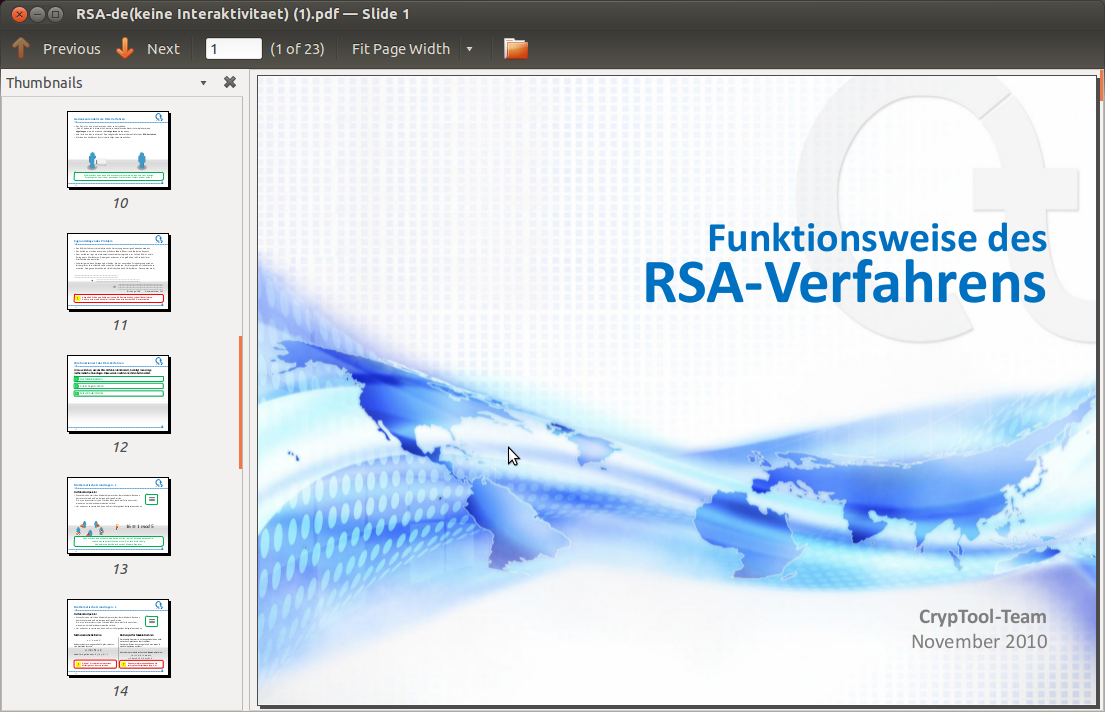
\includegraphics[scale=0.4]{figures/Interactive_RSA_Presentation_D.png}
\caption{Screenshot RSA-Präsentation (PDF)}
\label{l_Interactive_RSA_Presentation}
\end{center}
\end{figure}



% ++++++++++++++++++++++++++++++++++++++++++++++++++++++++++++++++++++++++++
\newpage
\hypertarget{NumberTheory_Appendix_E}{}
\section{Anhang: Beispiele mit SageMath}
\label{NumberTheory_Appendix_E}{}
\index{SageMath}
\index{SageMath!Programmbeispiele}

\begin{ctsquote}
\glqq Nie würde sie ihren Eltern ... von dieser ganzen Welt erzählen können. Nicht von ihrer Arbeit, die im Knacken von Codes bestand. Nicht vom Fiasko der Daemon-Taskforce ... Nicht von den schattenhaften Marionetten, die die Regierung nach ihrer Pfeife tanzen ließen.\grqq
\caption[Daniel Suarez]{Daniel Suarez\footnotemark}\index{Suarez, Daniel}
\end{ctsquote}
\addtocounter{footnote}{0}\footnotetext{Daniel Suarez, \glqq Darknet\grqq,
     rororo, (c) 2011, Kapitel 19, \glqq Scheideweg\grqq, S. 229, Philips.}


\noindent In diesem Anhang finden Sie SageMath-Quellcode, mit dem Sie die Tabellen und
Beispiele des Kapitels~\ref{Chapter_ElementaryNT}
(\glqq \nameref{Chapter_ElementaryNT}\grqq) berechnen können.


% ---------------------------------------------------------------------------
\hypertarget{nt:AppArith1}{}
\subsection{Multiplikationstabellen modulo m}
\label{nt:AppArith1}{}

Die Multiplikationstabelle~\ref{mulmod17} (von Seite \pageref{SrcArith1a})
für $a \times i \pmod{m}$, mit $m = 17$, $a=5$ and $a=6$, und $i$ von $0$ bis $16$
kann mit folgenden SageMath-Befehlen berechnet werden:

\begin{sagecode}
\begin{Verbatim}%
[fontsize=\footnotesize]
sage: m = 17; a = 5; b = 6
sage: [mod(a * i, m).lift() for i in xrange(m)]
[0, 5, 10, 15, 3, 8, 13, 1, 6, 11, 16, 4, 9, 14, 2, 7, 12]
sage: [mod(b * i, m).lift() for i in xrange(m)]
[0, 6, 12, 1, 7, 13, 2, 8, 14, 3, 9, 15, 4, 10, 16, 5, 11]
\end{Verbatim}
\caption{Multiplikationstabelle $a \times i \pmod{m}$ mit $m = 17$, $a=5$ and $a=6$}
\end{sagecode}

\noindent Die Funktion \verb!mod()! gibt das Objekt zurück, das die natürlichen
Zahlen modulo $m$ (in unserem Fall $m = 17$) repräsentiert.
Aus dem {\tt Mod}-Objekt kann man die einzelnen Komponenten entweder mit der
\texttt{component}- oder mit der \texttt{lift}-Funktion zurückgewinnen.
Wir nutzen hier die Methode \verb!lift()!, um das Objekt in eine Zahl umzuwandeln und
auszugeben.

Die weiteren Beispiele der Multiplikationstabelle modulo $13$ (Tabelle~\ref{mulmod13})
und modulo $12$ (Tabelle~\ref{mulmod12}) auf Seite \pageref{SrcArith1b}
kann man auf dieselbe Weise bestimmen, wenn man im Quelltext jeweils
{\tt m=17} durch den entsprechenden Zahlenwert ({\tt m=13} bzw. {\tt m=12}) ersetzt.


% ---------------------------------------------------------------------------
\vskip +25 pt
\hypertarget{nt:AppArith2}{}
\subsection{Schnelles Berechnen hoher Potenzen}
\label{nt:AppArith2}{}

Das schnelle Potenzieren modulo $m$ kann mit der SageMath-Funktion \verb!power_mod()!
durchgeführt werden. Das Ergebnis dieser Funktion ist eine natürliche Zahl.
Sie können mit Hilfe der folgenden Zeilen die Idee der Square-and-Multiply-Methode
nachvollziehen, wie sie im Beispiel in Kapitel \glqq \nameref{hohpot}\grqq~
auf Seite \pageref{SrcArith2} dargestellt ist:

\begin{sagecode}
\begin{Verbatim}%
[fontsize=\footnotesize]
sage: a = 87; m = 103
sage: exp = [2, 4, 8, 16, 32, 43]
sage: [power_mod(a, e, m) for e in exp]
[50, 28, 63, 55, 38, 85]
\end{Verbatim}
\caption{Schnelles Berechnen hoher Potenzen mod $m = 103$}
\end{sagecode}


% ---------------------------------------------------------------------------
\newpage
\hypertarget{nt:AppArith3a1}{}
\subsection{Multiplikative Ordnung}
\label{nt:AppArith3a1}{}

Die Ordnung $ord_m(a)$ einer Zahl $a$ in der multiplikativen Gruppe $Z_m^*$ ist
die kleinste natürliche Zahl $i \ge 1$ für die gilt $a^i \equiv 1$ mod $m$
(siehe Kapitel~\ref{MultOrdPrimitveRoot}, \glqq \nameref{MultOrdPrimitveRoot}\grqq).

Um die Tabelle~\ref{expmod11} auf Seite~\pageref{SrcArith3a} zu berechnen,
können wir alle Potenzen $a^i \pmod{11}$ wie folgt ausgeben:

\begin{sagecode}
\begin{Verbatim}%
[fontsize=\footnotesize]
sage: m = 11
sage: for a in xrange(1, m):
....:     print [power_mod(a, i, m) for i in xrange(1, m)]
....:
[1, 1, 1, 1, 1, 1, 1, 1, 1, 1]
[2, 4, 8, 5, 10, 9, 7, 3, 6, 1]
[3, 9, 5, 4, 1, 3, 9, 5, 4, 1]
[4, 5, 9, 3, 1, 4, 5, 9, 3, 1]
[5, 3, 4, 9, 1, 5, 3, 4, 9, 1]
[6, 3, 7, 9, 10, 5, 8, 4, 2, 1]
[7, 5, 2, 3, 10, 4, 6, 9, 8, 1]
[8, 9, 6, 4, 10, 3, 2, 5, 7, 1]
[9, 4, 3, 5, 1, 9, 4, 3, 5, 1]
[10, 1, 10, 1, 10, 1, 10, 1, 10, 1]

und die letzte Spalte ergänzt um die Ordnung des jeweiligen a mod (11)

sage: m = 11
sage: for a in xrange(1, m):
....:     lst= [power_mod(a, i, m) for i in xrange(1, m)]
....:     lst.append(multiplicative_order(mod(a,m)))
....:     print lst
....:
[1, 1, 1, 1, 1, 1, 1, 1, 1, 1, 1]
[2, 4, 8, 5, 10, 9, 7, 3, 6, 1, 10]
[3, 9, 5, 4, 1, 3, 9, 5, 4, 1, 5]
[4, 5, 9, 3, 1, 4, 5, 9, 3, 1, 5]
[5, 3, 4, 9, 1, 5, 3, 4, 9, 1, 5]
[6, 3, 7, 9, 10, 5, 8, 4, 2, 1, 10]
[7, 5, 2, 3, 10, 4, 6, 9, 8, 1, 10]
[8, 9, 6, 4, 10, 3, 2, 5, 7, 1, 10]
[9, 4, 3, 5, 1, 9, 4, 3, 5, 1, 5]
[10, 1, 10, 1, 10, 1, 10, 1, 10, 1, 2]
\end{Verbatim}
\caption{Tabelle mit allen Potenzen $a^i \pmod{m}$ für $m=11$, $a=1,...,10$}
\label{nt_Sage-code_MultOrder_expmod11}%Creates table with label expmod11
\end{sagecode}


\newpage
\hypertarget{nt:AppArith3b}{}
\label{nt:AppArith3b}{}
Die Tabelle~\ref{expmod45} auf Seite~\pageref{SrcArith3b} enthält Beispiele
für die Ordnung von a modulo 45 ($ord_{45}(a)$) und den Wert der Eulerfunktion
von 45 ($\phi(45)$).

Der folgende SageMath-Code erzeugt eine analoge Tabelle.

\begin{sagecode}
\begin{Verbatim}%
[fontsize=\footnotesize]
sage: m = 45
sage: for a in xrange(1, 13):
....:     lst = [power_mod(a, i, m) for i in xrange(1, 13)]
....:     try:
....:         lst.append(multiplicative_order(mod(a, m)))
....:     except:
....:         lst.append("None")
....:     lst.append(euler_phi(m))
....:     print lst
....:
[1, 1, 1, 1, 1, 1, 1, 1, 1, 1, 1, 1, 1, 24]
[2, 4, 8, 16, 32, 19, 38, 31, 17, 34, 23, 1, 12, 24]
[3, 9, 27, 36, 18, 9, 27, 36, 18, 9, 27, 36, 'None', 24]
[4, 16, 19, 31, 34, 1, 4, 16, 19, 31, 34, 1, 6, 24]
[5, 25, 35, 40, 20, 10, 5, 25, 35, 40, 20, 10, 'None', 24]
[6, 36, 36, 36, 36, 36, 36, 36, 36, 36, 36, 36, 'None', 24]
[7, 4, 28, 16, 22, 19, 43, 31, 37, 34, 13, 1, 12, 24]
[8, 19, 17, 1, 8, 19, 17, 1, 8, 19, 17, 1, 4, 24]
[9, 36, 9, 36, 9, 36, 9, 36, 9, 36, 9, 36, 'None', 24]
[10, 10, 10, 10, 10, 10, 10, 10, 10, 10, 10, 10, 'None', 24]
[11, 31, 26, 16, 41, 1, 11, 31, 26, 16, 41, 1, 6, 24]
[12, 9, 18, 36, 27, 9, 18, 36, 27, 9, 18, 36, 'None', 24]
\end{Verbatim}
\caption{Tabelle mit allen Potenzen $a^i \pmod{45}$ für $a=1,...,12$ plus der Ordnung von a}
\label{nt_Sage-code_MultOrder_expmod45}
\end{sagecode}

Die Ordnung $\text{ord}_m(a)$ kann nur berechnet werden, wenn $a$
teilerfremd\index{Zahlen!teilerfremd (co-prime)} zu $m$ ist.
Das kann mit der Abfrage, ob \verb!gcd(a, m)==1!, überprüft werden.

In unserem Codebeispiel haben wir stattdessen die Berechung der
multiplikativen Ordnung in einem \verb!try!-\verb!except!-Block
durchgeführt. Auf diese Weise kann SageMath jede Ausnahme und jeden Fehler
abfangen, der von der Funktion \verb!multiplicative_order()! geworfen wird.
Wird eine Ausnahmen oder ein Fehler im \verb!try!-Block geworfen, wissen
wir, dass $\text{ord}_m(a)$ nicht existiert für den gegebenen Wert von $a$.
Daher wird dann im \verb!except!-Block ans Ende der Zeile der String \verb!"None"!
angehängt (die Zeile wird durch das Objekt \verb!lst! repräsentiert).


\newpage
\hypertarget{nt:AppArith3c}{}
\label{nt:AppArith3c}{}
Die Tabelle~\ref{expmod46} auf Seite~\pageref{SrcArith3c} enthält Beispiele
für die Exponentiationen $a^i$ mod $46$ sowie die Ordnungen $ord_{46}(a)$

Der folgende SageMath-Code erzeugt eine analoge Tabelle.

\begin{sagecode}
\begin{Verbatim}%
[fontsize=\footnotesize]
sage: m = 46
sage: euler_phi(m)
22
sage: for a in xrange(1, 24):
....:     lst = [power_mod(a, i, m) for i in xrange(1, 24)]
....:     try:
....:         lst.append(multiplicative_order(mod(a, m)))
....:     except:
....:         lst.append("None")
....:     print lst
....:
[1, 1, 1, 1, 1, 1, 1, 1, 1, 1, 1, 1, 1, 1, 1, 1, 1, 1, 1, 1, 1, 1, 1, 1]
[2, 4, 8, 16, 32, 18, 36, 26, 6, 12, 24, 2, 4, 8, 16, 32, 18, 36, 26, 6, 12, 24, 2, 'None']
[3, 9, 27, 35, 13, 39, 25, 29, 41, 31, 1, 3, 9, 27, 35, 13, 39, 25, 29, 41, 31, 1, 3, 11]
[4, 16, 18, 26, 12, 2, 8, 32, 36, 6, 24, 4, 16, 18, 26, 12, 2, 8, 32, 36, 6, 24, 4, 'None']
[5, 25, 33, 27, 43, 31, 17, 39, 11, 9, 45, 41, 21, 13, 19, 3, 15, 29, 7, 35, 37, 1, 5, 22]
[6, 36, 32, 8, 2, 12, 26, 18, 16, 4, 24, 6, 36, 32, 8, 2, 12, 26, 18, 16, 4, 24, 6, 'None']
[7, 3, 21, 9, 17, 27, 5, 35, 15, 13, 45, 39, 43, 25, 37, 29, 19, 41, 11, 31, 33, 1, 7, 22]
[8, 18, 6, 2, 16, 36, 12, 4, 32, 26, 24, 8, 18, 6, 2, 16, 36, 12, 4, 32, 26, 24, 8, 'None']
[9, 35, 39, 29, 31, 3, 27, 13, 25, 41, 1, 9, 35, 39, 29, 31, 3, 27, 13, 25, 41, 1, 9, 11]
[10, 8, 34, 18, 42, 6, 14, 2, 20, 16, 22, 36, 38, 12, 28, 4, 40, 32, 44, 26, 30, 24, 10, 'None']
[11, 29, 43, 13, 5, 9, 7, 31, 19, 25, 45, 35, 17, 3, 33, 41, 37, 39, 15, 27, 21, 1, 11, 22]
[12, 6, 26, 36, 18, 32, 16, 8, 4, 2, 24, 12, 6, 26, 36, 18, 32, 16, 8, 4, 2, 24, 12, 'None']
[13, 31, 35, 41, 27, 29, 9, 25, 3, 39, 1, 13, 31, 35, 41, 27, 29, 9, 25, 3, 39, 1, 13, 11]
[14, 12, 30, 6, 38, 26, 42, 36, 44, 18, 22, 32, 34, 16, 40, 8, 20, 4, 10, 2, 28, 24, 14, 'None']
[15, 41, 17, 25, 7, 13, 11, 27, 37, 3, 45, 31, 5, 29, 21, 39, 33, 35, 19, 9, 43, 1, 15, 22]
[16, 26, 2, 32, 6, 4, 18, 12, 8, 36, 24, 16, 26, 2, 32, 6, 4, 18, 12, 8, 36, 24, 16, 'None']
[17, 13, 37, 31, 21, 35, 43, 41, 7, 27, 45, 29, 33, 9, 15, 25, 11, 3, 5, 39, 19, 1, 17, 22]
[18, 2, 36, 4, 26, 8, 6, 16, 12, 32, 24, 18, 2, 36, 4, 26, 8, 6, 16, 12, 32, 24, 18, 'None']
[19, 39, 5, 3, 11, 25, 15, 9, 33, 29, 45, 27, 7, 41, 43, 35, 21, 31, 37, 13, 17, 1, 19, 22]
[20, 32, 42, 12, 10, 16, 44, 6, 28, 8, 22, 26, 14, 4, 34, 36, 30, 2, 40, 18, 38, 24, 20, 'None']
[21, 27, 15, 39, 37, 41, 33, 3, 17, 35, 45, 25, 19, 31, 7, 9, 5, 13, 43, 29, 11, 1, 21, 22]
[22, 24, 22, 24, 22, 24, 22, 24, 22, 24, 22, 24, 22, 24, 22, 24, 22, 24, 22, 24, 22, 24, 22, 'None']
[23, 23, 23, 23, 23, 23, 23, 23, 23, 23, 23, 23, 23, 23, 23, 23, 23, 23, 23, 23, 23, 23, 23, 'None']
\end{Verbatim}
\caption{Tabelle mit allen Potenzen $a^i \pmod{46}$ für $a=1,...,23$ plus die Ordnung von a}
\label{nt_Sage-code_MultOrder_expmod46}
\end{sagecode}




\newpage
\hypertarget{nt:AppArith3d}{}
\label{nt:AppArith3d}{}
Der folgende Code für die Tabellen~\ref{expmod14} und~\ref{expmod22}
auf Seite~\pageref{expmod14} f. gibt auch gleich das Ergebnis so aus,
dass man es leicht in LaTeX weiter verarbeiten kann. Voraussetzung dafür ist,
dass alle Inhalte vorher einem SageMath-Objekt (hier einer Matrix) zugewiesen
werden.\footnote{%
        Anmerkungen zu dem SageMath-Programm, insbesondere den
        SageMath-Indizes\index{SageMath}\index{SageMath!latex()}:
        \begin{compactitem}
         \item for x in xrange(2, 5) liefert 2,3,4.
         \item m = matrix(ZZ, 2, 5) hat 2 Zeilen und 5 Spalten.\\
               Die Zellen haben die Bezeichner m(0,0) bis m(1,4).
         \item Alle Elemente der Matrix müssen numerisch sein, daher \glqq 0\grqq
               statt \glqq None\grqq.
         \item Die Ausgabe von Matrizen kann man in SageMath so steuern:
\begin{Verbatim}
               sage: from sage.matrix.matrix0 import set_max_cols, set_max_rows
               sage: set_max_cols(100)
               sage: set_max_rows(100)
\end{Verbatim}
         \item Die Zykluslänge in der letzten Spalte in den
               Tabellen~\ref{expmod14} und~\ref{expmod22}
               wurde noch von Hand ermittelt.
        \end{compactitem}
        \vspace{-\baselineskip} % Hier nötig, damit alles auf 1 Seite passt!
        }

\begin{sagecode}
\begin{Verbatim}%
[fontsize=\footnotesize]
def power_mod_order_matrix(m, max_a, max_i):
    r = matrix(ZZ, max_a+1, max_i+3)
    for a in xrange(0, max_a+1):
        r[a, 0] = a
        for i in xrange(1, max_i+1):
            if a==0:
                r[a,i] = i
            else:
                r[a, i] = power_mod(a, i, m)
        try:
            r[a, max_i+1] = multiplicative_order(mod(a, m))
        except:
            r[a, max_i+1] = 0
        r[a, max_i+2] = euler_phi(m)
    return r

print "\n1: m=45;max_i=13;max_a=13";m=45;max_i=13;max_a=13
r = power_mod_order_matrix(m, max_a, max_i);print r;print latex(r)

print "\n2: m=46;max_i=25;max_a=25";m=46;max_i=25;max_a=25
r = power_mod_order_matrix(m, max_a, max_i);print r.str();print latex(r)

print "\n3: m=14;max_i=13;max_a=16";m=14;max_i=13;max_a=16
r = power_mod_order_matrix(m, max_a, max_i);print r;print latex(r)

print "\n4: m=22;max_i=21;max_a=25";m=22;max_i=21;max_a=25
r = power_mod_order_matrix(m, max_a, max_i);print r.str();print latex(r)
...
3: m=14;max_i=13;max_a=16
[ 0  1  2  3  4  5  6  7  8  9 10 11 12 13  0  6]
[ 1  1  1  1  1  1  1  1  1  1  1  1  1  1  1  6]
[ 2  2  4  8  2  4  8  2  4  8  2  4  8  2  0  6]
[ 3  3  9 13 11  5  1  3  9 13 11  5  1  3  6  6]
...
\left(\begin{array}{rrrrrrrrrrrrrrrr}
0 & 1 & 2 & 3 & 4 & 5 & 6 & 7 & 8 & 9 & 10 & 11 & 12 & 13 & 0 & 6\\
1 & 1 & 1 & 1 & 1 & 1 & 1 & 1 & 1 & 1 & 1 & 1 & 1 & 1 & 1 & 6\\
2 & 2 & 4 & 8 & 2 & 4 & 8 & 2 & 4 & 8 & 2 & 4 & 8 & 2 & 0 & 6\\
3 & 3 & 9 & 13 & 11 & 5 & 1 & 3 & 9 & 13 & 11 & 5 & 1 & 3 & 6 & 6\\
...
\end{Verbatim}
\caption{Code für Tabellen mit allen Potenzen $a^i \pmod{m}$ für variable $a$ und $i$ plus Ordnung von a und Eulerphi von m}
\end{sagecode}




% ---------------------------------------------------------------------------
\newpage
\hypertarget{nt:AppArith3a2}{}
\subsection{Primitivwurzeln}
\label{nt:AppArith3a2}
\label{primitive-roots-with-sage}
\index{Primitivwurzel}

Das Berechnen von Primitivwurzeln
(siehe Kapitel~\ref{MultOrdPrimitveRoot}, \glqq \nameref{MultOrdPrimitveRoot}\grqq)
geht in SageMath sehr einfach: Sei \verb!n! eine natürliche Zahl, dann kann mit dem Befehl
\verb!primitive_root(n)! \textit{eine} Primitivwurzel der multiplikativen Gruppe
$(\mathbf{Z} / n \mathbf{Z})^{\ast}$ berechnet werden, sofern eine existiert.
Ist $n$ prim, dann ist das äquivalent zum Berechnen einer Primitivwurzel in
$\mathbf{Z} / n \mathbf{Z}$.

\noindent Im folgenden berechnen wir die Primitivwurzeln einiger natürlicher Zahlen.

\begin{sagecode}
\begin{Verbatim}%
[fontsize=\footnotesize]
sage: primitive_root(4)
3
sage: primitive_root(22)
13
sage: for p in primes(1, 50):
....:     print p, primitive_root(p)
....:
2 1
3 2
5 2
7 3
11 2
13 2
17 3
19 2
23 5
29 2
31 3
37 2
41 6
43 3
47 5
\end{Verbatim}
\caption{Berechnen einer Primitivwurzel für eine gegebene Primzahl}
\end{sagecode}

\noindent Ist $p$ prim, dann hat $\mathbf{Z} / p \mathbf{Z}$ mindestens eine Primitivwurzel.\\



\newpage
\noindent Will man \texttt{alle} Primitivwurzeln von $(\mathbf{Z} / n \mathbf{Z})^{\ast}$
berechnen, und nicht nur irgend eine einzige von $(\mathbf{Z} / n \mathbf{Z})^{\ast}$,
dann kann man das mit der folgenden selbstgeschriebenen Funktion durchführen.%
\footnote{Der folgende Code wurde als SageMath-Skriptdatei erstellt und
  nicht-interaktiv ausgeführt. Deshalb gibt es in der Ausgabe keine Zeilen,
  die mit \glqq sage:\grqq~oder
  \glqq ....:\grqq~anfangen wie in den SageMath-Programmbeispielen bisher.
}

%\newpage %BERM_Warning: Egal, ob Newpage hier oder vor dem Text (wie im Englischen): Warum gibt
         %              es nur im Deutschen die Warnung: "Text page 202 contains only floats."
\begin{sagecode}
\begin{Verbatim}%
[fontsize=\footnotesize]
def enum_PrimitiveRoots_of_an_Integer(M):
    r"""
    Return all the primitive roots of the integer M (if possible).
    """
    try:
        g = primitive_root(M)
    except:
        return None
    targetOrder = euler_phi(M)
    L=[]
    # Stepping through all odd integers from 1 up to M, not including
    # M. So this loop only considers values of i where 1 <= i < M.
    for i in xrange(1,M,2):
            testGen = Mod(g^i,M)
            if testGen.multiplicative_order() == targetOrder:
                L.append(testGen.lift())
    # removing duplicates
    return Set(L)

# AA_Start -- Testcases for enum_PrimitiveRoots_of_an_Integer(M)
print "AA_Start -- Testcases for enum_PrimitiveRoots_of_an_Integer(M)"
M=10; print "1-----------Testcase: M = %s" % M
LL = enum_PrimitiveRoots_of_an_Integer(M)
if LL==None:
    print M
else:
    print LL
M=8; print "2-----------Testcase: M = %s" % M
# M=8 hat keine primitive root mod m. Checke, ob per try - except abgefangen.
LL = enum_PrimitiveRoots_of_an_Integer(M)
if LL==None:
    print M
else:
    print LL
M=17; print "3-----------Testcase: M = %s" % M
LL = enum_PrimitiveRoots_of_an_Integer(M)
if LL==None:
    print M
else:
    print LL
# AA_End -- Testcases

OUTPUT:
AA_Start -- Testcases for enum_PrimitiveRoots_of_an_Integer(M)
1-----------Testcase: M = 10
{3, 7}
2-----------Testcase: M = 8
8
3-----------Testcase: M = 17
{3, 5, 6, 7, 10, 11, 12, 14}
\end{Verbatim}
\caption{Funktion \glqq enum\_PrimitiveRoots\_of\_an\_Integer\grqq~zur Berechnung
         aller Primitiv\-wurzeln für eine gegebene Zahl}
\end{sagecode}



\newpage
\noindent Das folgende Beispiel listet alle Primitivwurzeln der Primzahl 541 auf.

\begin{sagecode}
\begin{Verbatim}%
[fontsize=\footnotesize]
sage: L=enum_PrimitiveRoots_of_an_Integer(541); L
{2, 517, 10, 523, 13, 14, 527, 528, 18, 531, 24, 539, 30, 37, 40, 51,
54, 55, 59, 62, 65, 67, 68, 72, 73, 77, 83, 86, 87, 91, 94, 96, 98,
99, 107, 113, 114, 116, 117, 126, 127, 128, 131, 132, 138, 150, 152,
153, 156, 158, 163, 176, 181, 183, 184, 195, 197, 199, 206, 208,
210, 213, 218, 220, 223, 224, 244, 248, 250, 257, 258, 259, 260,
261, 263, 267, 269, 270, 271, 272, 274, 278, 280, 281, 282, 283,
284, 291, 293, 297, 317, 318, 321, 323, 328, 331, 333, 335, 342,
344, 346, 357, 358, 360, 365, 378, 383, 385, 388, 389, 391, 403,
409, 410, 413, 414, 415, 424, 425, 427, 428, 434, 442, 443, 445,
447, 450, 454, 455, 458, 464, 468, 469, 473, 474, 476, 479, 482,
486, 487, 490, 501, 504, 511}
sage: len(L)
144
\end{Verbatim}
\caption{Tabelle mit allen Primitivwurzeln der vorgegebenen Primzahl 541}
\end{sagecode}



\newpage
\noindent Mit etwas Programmieren kann man zählen, wie viele Primitivwurzeln
es gibt für alle natürlichen Zahlen in einem gegebenen Zahlenbereich.
Wir können das für alle Zahlen oder nur für die Primzahlen in diesem Bereich berechnen.

\begin{sagecode}
\begin{Verbatim}%
[fontsize=\footnotesize]
def count_PrimitiveRoots_of_an_IntegerRange(start, end, bPrimesOnly=True):
	r"""
	Compute all primitive roots of all numbers between start and end,
	inclusive, and count them.
	If the flag bPrimesOnly is True, it performs primality tests, so it
	allows us to count the number of primes from start to end, inclusive.
        If the flag bPrimesOnly is false, it additionally counts these even
	numbers which have no primitive root.
	"""
	nCheckedNumb = 0
	nCheckedNumb_WithoutPrimitivRoots = 0
	nPrimitiveRoots = 0
	for n in xrange(start, end+1):
		if bPrimesOnly:
			if is_prime(n):
				nCheckedNumb += 1
				L = enum_PrimitiveRoots_of_an_Integer(n)
				nPrimitiveRoots += len(L)
		else:
			nCheckedNumb += 1
			L = enum_PrimitiveRoots_of_an_Integer(n)
			if L==None:
				nCheckedNumb_WithoutPrimitivRoots += 1
			else:
				nPrimitiveRoots += len(L)

	if bPrimesOnly:
		print "Found all %s" % nPrimitiveRoots + \
		      " primitive roots of %s primes." % nCheckedNumb
	else:
		if nCheckedNumb_WithoutPrimitivRoots == 0:
			print "Found all %s " % nPrimitiveRoots + \
			      "primitive roots of %s numbers." % nCheckedNumb
		else:
			print "Found all %s " % nPrimitiveRoots + \
			      "primitive roots of %s numbers." % \
			          (nCheckedNumb - nCheckedNumb_WithoutPrimitivRoots)
			print "(Total of numbers checked: %s, " % nCheckedNumb + \
			      "Amount of numbers without primitive roots: %s)" % \
			          nCheckedNumb_WithoutPrimitivRoots
\end{Verbatim}
\caption{Funktion \glqq count\_PrimitiveRoots\_of\_an\_IntegerRange\grqq~zur Berechnung
         aller Pri\-mitivwurzeln für einen gegebenen Zahlenbereich}
\end{sagecode}


\newpage
\noindent Um zu sehen, wie lange unser Computer für diese Berechnung braucht,
kann man den SageMath-Befehl \verb!time! verwenden.

\begin{sagecode}
\begin{Verbatim}%
[fontsize=\footnotesize]
# BB_Start -- Testcases for count_PrimitiveRoots_of_an_IntegerRange(start, end, bPrimesOnly=True)
print "\n\nBB_Start -- Testcases for count_PrimitiveRoots_of_an_IntegerRange(start, end, True)"

print "\n1-----------Testcase: (1, 500)"
time count_PrimitiveRoots_of_an_IntegerRange(1, 500)

print "\n2-----------Testcase: (5, 6, False)"
time count_PrimitiveRoots_of_an_IntegerRange(5, 6, False)

print "\n3-----------Testcase: (1, 500, False)"
time count_PrimitiveRoots_of_an_IntegerRange(1, 500, False)
# BB_End -- Testcases

OUTPUT:
BB_Start -- Testcases for count_PrimitiveRoots_of_an_IntegerRange(start, end, bPrimesOnly=True)

1-----------Testcase: (1, 500)
Found all 8070 primitive roots of 95 primes.
Time: CPU 0.94 s, Wall: 0.97 s

2-----------Testcase: (5, 6, False)
Found all 3 primitive roots of 2 numbers.
Time: CPU 0.00 s, Wall: 0.00 s

3-----------Testcase: (1, 500, False)
Found all 11010 primitive roots of 170 numbers.
(Total of numbers checked: 500, Amount of numbers without primitive roots: 330)
Time: CPU 1.52 s, Wall: 1.59 s
\end{Verbatim}
\caption{Funktion \glqq count\_PrimitiveRoots\_of\_an\_IntegerRange\grqq: Testfälle und Testausgaben}
\end{sagecode}




\clearpage
\noindent Mit unserer selbst erstellten Funktion \verb!enum_PrimitiveRoots_of_an_Integer!
kann man alle Primitivwurzeln einer Primzahl $p$ finden.

Die folgende Funktion zählt, wie viele Primitivwurzeln es innerhalb eines Primzahl-Bereiches
gibt, und listet diese Primitivwurzeln jeweils auf.

Aus dieser Liste der Primitivwurzeln können wir jeweils die kleinste und größte
Primitivwurzel pro $\mathbf{Z} / p \mathbf{Z}$ bestimmen, als auch die Anzahl von
Primitivwurzeln pro $\mathbf{Z} / p \mathbf{Z}$ zählen.

\begin{sagecode}
\begin{Verbatim}%
[fontsize=\footnotesize]
def count_PrimitiveRoots_of_a_PrimesRange(start, end):
      r"""
      Compute all primitive roots of all primes between start and end,
      inclusive. This uses a primes iterator.
      """
      nPrimes = 0
      nPrimitiveRoots = 0
      for p in primes(start, end+1):
          L = enum_PrimitiveRoots_of_an_Integer(p)
	  print p, len(L)
          nPrimes += 1
          nPrimitiveRoots += len(L)
      print "Found all %s" % nPrimitiveRoots + " primitive roots of %s primes." % nPrimes

# CC_Start -- Testcases for count_PrimitiveRoots_of_a_PrimesRange(start, end)
print "\n\nBB_Start -- Testcases for count_PrimitiveRoots_of_a_PrimesRange(start, end)"
print "-----------Testcase: (1, 1500)"
time count_PrimitiveRoots_of_a_PrimesRange(1, 1500)
# CC_End -- Testcases

OUTPUT:
CC_Start -- Testcases for count_PrimitiveRoots_of_a_PrimesRange(start, end)
-----------Testcase: (1, 1500)
2 1
3 1
5 2
7 2
11 4
13 4
17 8
19 6
23 10
29 12
31 8
37 12
...
1483 432
1487 742
1489 480
1493 744
1499 636
Found all 62044 primitive roots of 239 primes.
Time: CPU 7.55 s, Wall: 7.85 s
\end{Verbatim}
\caption{Funktion \glqq count\_PrimitiveRoots\_of\_a\_PrimesRange\grqq~zur Berechnung
         aller Primitivwurzeln für ein gegebenes Intervall von Primzahlen}
\end{sagecode}



\newpage
\noindent Die Funktion \verb!count_PrimitiveRoots_of_a_PrimesRange! wurde von
Minh Van Nguyen leicht geändert, um eine Liste (Datenbank) aller Primitivwurzeln
für alle Primzahlen zwischen 1 und 100.000 zu erstellen.

\begin{sagecode}
\begin{Verbatim}%
[fontsize=\footnotesize]
start = 1
end = 10^5
fileName = "./primroots.dat"
file = open(fileName, "w")
for p in primes(start, end+1):
    L = enum_PrimitiveRoots_of_an_Integer(p)
    print p, len(L)
    # Output to a file. The format is:
    # (1) the prime number p under consideration
    # (2) the number of primitive roots of Z/pZ
    # (3) all the primitive roots of Z/pZ
    file.write(str(p) + " " + str(len(L)) + " " + str(L) + "\n")
    file.flush()
file.close()
\end{Verbatim}
\caption{Code zur Erstellung einer Liste mit allen Primitivwurzeln für alle Primzahlen
         zwischen 1 und 100.000}
\end{sagecode}

Auch dieser Code und die Funktion \verb!enum_PrimitiveRoots_of_an_Integer!
wurden mit einer Sage-Skriptdatei nicht-interaktiv ausgeführt.
Die Ausführung dauerte mit SageMath 7.2 auf einem modernen PC rund 6 h.

Im Bereich 1 bis 100.000 liegen 9.592 Primzahlen. Für sie wurden insgesamt mehr als
169 Millionen Primitivwurzeln berechnet. Für jede Primzahl $p>3$ gilt, dass zwischen
20 \% und knapp 50 \% aller Zahlen zwischen 1 und p eine Primitivwurzel davon darstellen.
%%%%% Oder anders:
% Theorem: If p is a prime, then there is a primitive root for p.
% (In fact, if p is a prime and p>2, there are always at least two primitive roots,
% and sometimes many more.)
% The proof of this theorem is hard. It's in our ??? text (9.2?) and in
% second-semeter abstract algebra.

Die resultierende Datei \glqq primroots\_1-100000.dat\grqq~enthält die Liste
% Either mask _ within brackets, or use \verb!!primroots_1-100000.dat!
aller Primitivwurzeln für alle Primzahlen zwischen 1 und 100.000 inklusive.
Dies ist eine große Datei (ca. 1,1 GB unkomprimiert, und 156 MB komprimiert mit 7Zip).
Die komprimierte Datei kann abgerufen werden unter\\
\url{https://www.cryptool.org/images/ctp/documents/primroots_1-100000.7z}.

Ihr Inhalt sieht wie folgt aus:
\begin{Verbatim}%
[fontsize=\footnotesize]
2      1      {1}
3      1      {2}
5      2      {2, 3}
7      2      {3, 5}
11     4      {8, 2, 6, 7}
...
99989  42840  {2, 3, 8, 10, 11, 13, 14, ..., 99978, 99979, 99981, 99986, 99987}
99991  24000  {65539, 6, 65546, 11, 12, ..., 65518, 65520, 87379, 65526, 65528}
\end{Verbatim}




\newpage
Das Sage-Skript \ref{l:Sagecode_SmallestPrimRoot} berechnet für jede Primzahl (bis \glqq end\grqq)
alle Primitivwurzeln, und gibt jeweils die Anzahl unterschiedlicher
Primitivwurzeln und die jeweils kleinste Primitivwurzel aus.

\begin{sagecode}
\begin{Verbatim}%
[fontsize=\footnotesize]
start = 1
end = 10^6
fileName = "./primroot-smallest_up-to-one-million.dat"
file = open(fileName, "w")
file.write(timestring + "\n")
file.flush()
for p in primes(start, end+1):
	L = enum_PrimitiveRoots_of_an_Integer(p)
	# Output to commandline only p and number of prim roots of Z_p
	print p, len(L)
	# Output more to a file. The format is:
	# (1) the prime number p under consideration
	# (2) the number of primitive roots of Z_p
	# (3) the smallest primitive roots of Z_p
        LL = sorted(L) # necessary as the smallest primroot is not always
	               # found first by the enum fct (see L of p=43)
	file.write(str(p) + " " + str(len(L)) + " " + str(LL[0]) + "\n")
	file.flush()
file.flush()
file.close()
\end{Verbatim}
\caption{Code zur Erstellung einer Liste der jeweils kleinsten Primitivwurzeln für
	alle Primzahlen zwischen 1 und 1.000.000}
\label{l:Sagecode_SmallestPrimRoot}{}
\end{sagecode}

Das Sage-Skript \ref{l:Sagecode_SmallestPrimRoot} wurde nach mehreren Wochen
gestoppt (wo es auf einem modernen PC mit SageMath 7.2 lief), nachdem es alle
Primzahlen bis zu einer halben Million auswertete. Das Ergebnis wurde in der
Datei \glqq primroot\_number-of-and-smallest\_up-to-prime-500107.dat\grqq~gespeichert
(sie ist unkomprimiert 617 kB groß, und 178 kB komprimiert mit 7Zip).

Die komprimierte Datei kann abgerufen werden unter
%%% \url{https://www.cryptool.org/images/ctp/documents/primroot-smallest_up-to-one-million.7z}.
\url{https://www.cryptool.org/images/ctp/documents/primroot_number-of-and-smallest_up-to-prime-500107.7z}.

Diese Datenbank enthält für jede einzelne Primzahl p zwischen 1 und 500.107
die Anzahl der zugehörigen Primitivwurzeln und die kleinste Primitivwurzel mod p.
Es gilt, dass die Anzahl der Primitivwurzeln (für $p>3$) immer gerade ist.
Eine Formel, die die Anzahl der Primitivwurzeln zu einer Zahl angibt, kennen wir nicht.
Diese Datenbank könnte für Zahlentheoretiker interessant sein.\footnote{%
  Siehe auch Re: [sage-devel] What can we do with a database of primitive roots?\\
  \url{https://groups.google.com/forum/m/#!topic/sage-devel/TA5Nk2GdhOI}
}
% David Joyner mentions in his answer in [sage-devel]:
% "Least primitive root of prime numbers"
% http://plouffe.fr/simon/articles/Least%20primitive%20root%20of%20prime%20numbers.pdf
% Tomás Oliveira e Silva  October 21, 2004 (Universidade de Aveiro, PORTUGAL)
%
% Vgl. später auch mal:
% - http://wstein.org/edu/124/lectures/lecture11/lecture11.tex
% - http://www.aw-bc.com/rosen/weblinkch9.html   Annotated Web Links to
%   CHAPTER 9 - Primitive Roots in Elementary Number Theory, 5/E by
%   Kenneth H. Rosen, AT&T Laboratories, Publisher: Addison-Wesley, 2005, 744 pages
% - http://arxiv.org/pdf/0810.2325.pdf
%   A NOTE ON ARTIN’S CONSTANT  by  IVAN CHEREDNIK
% xxxxxxxxxxxxxxxxxxxxxxxxxxxxxxxxxxxxxx
%
Ihr Inhalt sieht wie folgt aus:
\begin{Verbatim}%xxxxxxxxxxx
[fontsize=\footnotesize]
2       1       1
3       1       2
5       2       2
7       2       3
11      4       2
13      4       2
17      8       3
...
99989   42840   2
99991   24000   6
100003  28560   2
...
500069  250032  2
500083  151520  2
500107  156864  2
\end{Verbatim}


\vskip +20 pt
Wenn man pro Primzahl nur die kleinste Primitivwurzel sucht, kann man dieses Skript
drastisch beschleunigen, indem man anhand der Theorie die möglichen Kandidaten direkter
sucht (anstatt mit \verb!enum_PrimitiveRoots_of_an_Integer! erstmal alle Primroots zu
generieren).






% \newpage
\clearpage
\noindent Die Datei \glqq primroots\_1-100000.dat\grqq~wurde dann als Input benutzt,
um mit dem folgenden Code (Sage-Skript \ref{l:Sagecode_Graphics-Distribution-PrimRoots})
drei Grafiken zu erstellen.

\begin{sagecode}
\begin{Verbatim}%
[fontsize=\footnotesize]
sage: # open a database file on primitive roots from 1 to 100,000
sage: file = open("/scratch/mvngu/primroots.dat", "r")
sage: plist = []    # list of all primes from 1 to 100,000
sage: nlist = []    # number of primitive roots modulo prime p
sage: minlist = []  # smallest primitive root modulo prime p
sage: maxlist = []  # largest primitive root modulo prime p
sage: for line in file:
....:     # get a line from the database file and tokenize it for processing
....:     line = line.strip().split(" ", 2)
....:     # extract the prime number p in question
....:     plist.append(Integer(line[0]))
....:     # extract the number of primitive roots modulo p
....:     nlist.append(Integer(line[1]))
....:     # extract the list of all primitive roots modulo p
....:     line = line[-1]
....:     line = line.replace("{", "")
....:     line = line.replace("}", "")
....:     line = line.split(", ")
....:     # sort the list in non-decreasing order
....:     line = [Integer(s) for s in line]
....:     line.sort()
....:     # get the smallest primitive root modulo p
....:     minlist.append(line[0])
....:     # get the largest primitive root modulo p
....:     maxlist.append(line[-1])
....:
sage: file.close()  # close the database file
sage: # plot of number of primitive roots modulo p
sage: nplot = point2d(zip(plist, nlist), pointsize=1)
sage: nplot.axes_labels(["x", "y"])
sage: nplot
sage: # plot of smallest primitive root modulo prime p
sage: minplot = point2d(zip(plist, minlist), pointsize=1)
sage: minplot.axes_labels(["x", "y"])
sage: minplot
sage: # plot of largest primitive root modulo prime p
sage: maxplot = point2d(zip(plist, maxlist), pointsize=1)
sage: maxplot.axes_labels(["x", "y"])
sage: maxplot
\end{Verbatim}
\caption{Code zur Erzeugung der Grafiken zur Verteilung der Primitivwurzeln}
\label{l:Sagecode_Graphics-Distribution-PrimRoots}{}
\end{sagecode}




\newpage
Abbildung~\ref{fig:primitive_roots_all} gibt die Anzahl der Primitivwurzeln
für jede Primzahl zwischen 1 und 100.000 aus. Die $x$-Achse repräsentiert
die Primzahlen 1 bis 100.000, die $y$-Achse gibt die Anzahl der Primitivwurzeln
pro Primzahl aus.

\begin{figure}[!htbp]
\centering
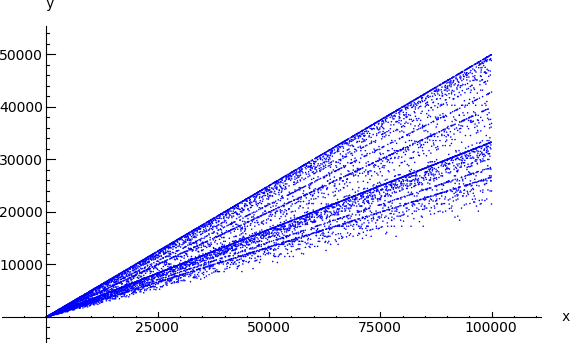
\includegraphics{figures/primitive-roots-all}
\caption{Die Anzahl der Primitivwurzeln für alle Primzahlen zwischen 1 und 100.000}
\label{fig:primitive_roots_all}
\end{figure}

\vskip +50 pt
Abbildung~\ref{fig:primitive_roots_smallest} gibt die kleinste Primitivwurzel
von jeder Primzahl zwischen 1 und 100.000 aus. Die $x$-Achse repräsentiert
die Primzahlen 1 bis 100.000, die $y$-Achse gibt die kleinste Primitivwurzel
pro Primzahl aus.

\vskip +25 pt
Abbildung~\ref{fig:primitive_roots_largest} zeigt die entsprechende Grafik
mit der größten Primitivwurzel zu jeder Primzahl im obigen Intervall.

\begin{figure}[!htbp]
\centering
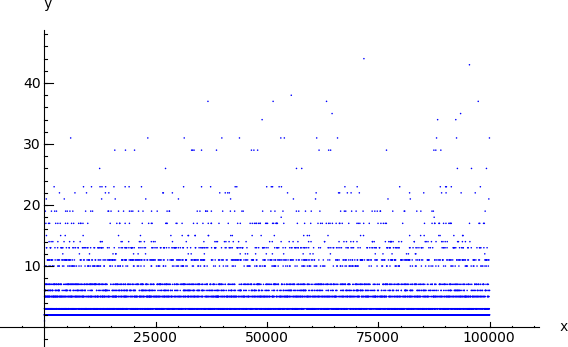
\includegraphics{figures/primitive-roots-smallest.png}
\caption{Die kleinste Primitivwurzel von jeder Primzahl zwischen 1 und 100.000}
\label{fig:primitive_roots_smallest}
\end{figure}

\begin{figure}[!htbp]
\centering
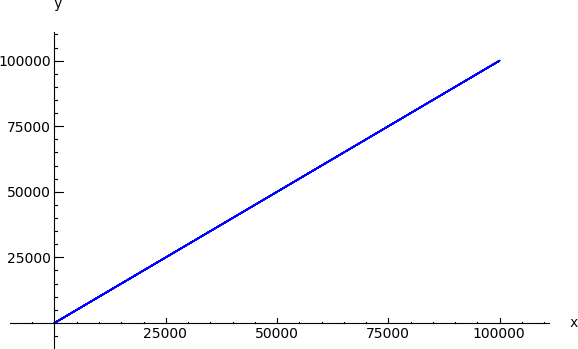
\includegraphics{figures/primitive-roots-largest.png}
\caption{Die größte Primitivwurzel von jeder Primzahl zwischen 1 und 100.000}
\label{fig:primitive_roots_largest}
\end{figure}

% To enforce that the next chapter starts at the beginning of a new page after
% the freely placed graphics, it was necessary to have TWO newpages and in between
% something to be printed (here invisible blanks).
% \newpage
% $ $
% I guess \clearpage is preferable.



% ---------------------------------------------------------------------------
\newpage
\hypertarget{NumberTheory_Sage_RSA_sample}{}
\subsection{RSA-Beispiele mit SageMath}
\label{l:NumberTheory_Sage_RSA_sample}{}

\noindent In diesem Abschnitt sind die SageMath-Quelltexte für die einfachen RSA-Beispiele
im Kapitel~\ref{rsaconcrete} (\glqq \nameref{rsaconcrete}\grqq) angegeben.

\vskip +10 pt
\hypertarget{nt:AppArith4a}{%
\noindent \textbf{Beispiel auf Seite~\pageref{SrcArith4a}:}}
\label{nt:AppArith4a}\\
Die RSA-Exponentiation $M^{37} \pmod{3713}$ für die Nachricht $M = 120$ kann
mit SageMath folgendermaßen ausgeführt werden:

\begin{Verbatim}%
[fontsize=\footnotesize]
sage: power_mod(120, 37, 3713)
1404
\end{Verbatim}


\vskip +10 pt
\hypertarget{nt:AppArith4b}{%
\noindent \textbf{Beispiel auf Seite~\pageref{SrcArith4b}:}}
\label{nt:AppArith4b}\\
Die Faktorisierung von $\phi(256.027) = 255.016 = 2^3 * 127 * 251$ kann mit SageMath
folgendermaßen durchgeführt werden:

\begin{sagecode}
\begin{Verbatim}%
[fontsize=\footnotesize]
sage: factor(255016)
2^3 * 127 * 251
\end{Verbatim}
\caption{Faktorisierung einer Zahl}
\end{sagecode}


\vskip +10 pt
\hypertarget{nt:AppArith4c}{%
\noindent \textbf{Beispiel auf Seite~\pageref{SrcArith4c}:}}
\label{nt:AppArith4c}\\
RSA-Verschlüsselung mit SageMath:

\begin{sagecode}
\begin{Verbatim}%
[fontsize=\footnotesize]
sage: A = [82, 83, 65, 32, 119, 111, 114, 107, 115, 33]
sage: e = 65537; m = 256027
sage: [power_mod(a, e, m) for a in A]
[212984, 25546, 104529, 31692, 248407, 100412, 54196, 100184, 58179, 227433]
\end{Verbatim}
\caption{RSA-Verschlüsselung durch modulare Exponentiation einer Zahl (als Nachricht)}
\end{sagecode}


\vskip +10 pt
\hypertarget{nt:AppArith4d}{%
\noindent \textbf{Beispiel auf Seite~\pageref{SrcArith4d}:}}
\label{nt:AppArith4d}\\
RSA-Verschlüsselung mit SageMath:

\begin{Verbatim}%
[fontsize=\footnotesize]
sage: A = [21075, 16672, 30575, 29291, 29473]
sage: e = 65537; m = 256027
sage: [power_mod(a, e, m) for a in A]
[158721, 137346, 37358, 240130, 112898]
\end{Verbatim}


\vskip +10 pt
\hypertarget{nt:AppArith4e}{%
\noindent \textbf{Beispiel auf Seite~\pageref{SrcArith4e}:}}
\label{nt:AppArith4e}\\
RSA-Verschlüsselung mit SageMath:

\begin{Verbatim}%
[fontsize=\footnotesize]
sage: A = [82083, 65032, 119111, 114107, 115033]
sage: e = 65537; m = 256027
sage: [power_mod(a, e, m) for a in A]
[198967, 51405, 254571, 115318, 14251]
\end{Verbatim}




% ---------------------------------------------------------------------------
\newpage
\hypertarget{NumberTheory_Sage_Number-of-RSA-keys}{}
%\subsection{Wie viele private RSA-Schlüssel gibt es innerhalb eines Modulo-Bereiches?}
% \texorpdfstring{$d$}{d} not necessary as title-id and title-output separated.
% \subsection[Wie viele private RSA-Schlüssel \texorpdfstring{$d$}{d} gibt es innerhalb eines Modulo-Bereiches?]
\subsection[Wie viele private RSA-Schlüssel d gibt es innerhalb eines Modulo-Bereiches?]
{Wie viele private RSA-Schlüs\discretionary{-}{}{}sel $d$ gibt es innerhalb eines Modulo-Be\-rei\-ches?}

\label{l:NumberTheory_Sage_Number-of-RSA-keys}{}

Die RSA-Verschlüsselung wurde beschrieben in Abschnitt \ref{RSA} (\glqq \nameref{RSA}\grqq).
Schritt 1 bis 3 definieren die Schlüsselerzeugung, Schritt 4 und 5 stellen die
eigentliche Verschlüsselung dar:
\begin{itemize}
  \item[\textbf{1.}] Wähle zwei unterschiedliche Primzahlen $p$ and $q$
                  und berechne $n = p*q$.\\
                  Der Wert $n$ wird RSA-Modul genannt.

  \item[\textbf{2.}] Wähle ein zufälliges $e \in \{2, \cdots, n-1\}$, so dass gilt:\\
                  $e$ ist relativ prim
                  \index{Primzahl!relativ}\index{Zahlen!relativ prim}
                  zu $\phi(n) = (p-1)*(q-1)$.\\
                  Danach kann man $p$ und $q$ \glqq wegwerfen\grqq.

  \item[\textbf{3.}] Wähle $d \in \{1, \cdots, n-1\}$ mit $e*d \equiv 1
                  {\rm ~(mod~} \phi(n))$,\\
		  d.h. $d$ ist die multiplikative Inverse von $e$ modulo $\phi(n)$.
		  Dann kann man $\phi(n)$ \glqq wegwerfen\grqq.
    \begin{compactitem}
      \item[] $\rightarrow (n, e)$ ist der öffentliche Schlüssel $P$.
      \item[] $\rightarrow (n, d)$ ist der private Schlüssel $S$ (nur $d$ muss man geheim halten).
    \end{compactitem}

  \item[\textbf{4.}] Zur Verschlüsselung wird die Nachricht als (binäre) Ziffernfolge
                  geschrieben. Diese Ziffernfolge wird dann so in gleich lange
                  Teilfolgen aufgeteilt, dass jede Teilfolge eine Zahl kleiner als
                  $n$ darstellt.

  \item[\textbf{5.}] Vorgang der Verschlüsselung auf dem Klartext (bzw. auf Teilen davon)
                  $M \in \{1, \cdots, n-1\}$:
                  $$C = E ( (n, e); M ) := M^e {\rm ~(mod~} n).$$
\end{itemize}

Standardmäßig versucht man, einen mit RSA verschlüsselten Geheimtext $C$
dadurch zu knacken, dass man den öffentlichen Schlüssel des Empfängers
betrachtet und versucht, $n$ zu faktorisieren. Hat man das erreicht, geht man
wieder durch die Schritte 2 und 3 und erzeugt den privaten Schlüssel $e$, den
man zum Entschlüsseln des Geheimtextes braucht.

Gemäß dem \glqq Primzahlsatz\grqq\footnote{%
Siehe Abschnitt \ref{thm-pz-pi-x} \glqq (\nameref{l_Primes_Distrib-of-Primes}\grqq).
% Der Ausdruck \nameref{thm-pz-pi-x}\grqq lieferte nur einen leeren String.
}
geht die Anzahl der Primzahlen $PI(x)$ asymptotisch gegen $x / ln(x)$.
Zwischen $1$ und einem gegebenen $n$ gibt es also ca. $n / ln(n)$ unterschiedliche
Primzahlen.

\noindent Will man nicht faktorisieren, sondern stellt sich eine Frage ähnlich
wie bei den klassischen Verschlüsselungsverfahren, kann man herausfinden wollen:
Wie viele verschiedene private Schlüssel $(n, d)$ gibt es für einen bestimmten
Bereich der Schlüsselgröße $n \in [a, b]$?\footnote{%
Kapitel~\ref{L_nt_Num-of-d-mod-26} (\glqq \nameref{L_nt_Num-of-d-mod-26}\grqq),
S.~\pageref{L_nt_Num-of-d-mod-26} behandelt den Spezialfall $n=26$.
}

\newpage
\noindent Das SageMath-Programm~\ref{nt_sagesample_Count_RSA_Keys} unten
definiert die Funktion \verb#count_Number_of_RSA_Keys#, die diese Frage konkret
beantwortet (wenn der Modulus nicht zu groß ist).\footnote{%
%\begin{compactitem}
\newlength{\saveleftmargini}
\setlength{\saveleftmargini}{\leftmargini}
\setlength{\leftmargini}{0em}% for example to outdent verse
\settowidth{\versewidth}{xxxxx xxxxx xxxxx xxxxx xxxxx xxxxx xxxxx xxxxx xxxxx xxxxx xxxxx xxxxx xxxxx xxxxx xxxxx xxxxx xxxxx xxxxx}
\vspace{-\baselineskip} % TODO_LaTeX: Geht das nicht anders?
\begin{verse}[\versewidth]
 a) Der Aufruf \verb#sage: count_Number_of_RSA_Keys(100, 1000)# bedeutet, dass
man das Intervall $[100, 1000]$ für $n$ betrachtet.
$n$ war definiert durch die beiden Primzahlen $p, q: n = p*q$.
\verselinebreak Daher kann hier die eine Primzahl höchstens den Wert $500$ annehmen, weil
$2 * 500 =1000$ (d.h. wenn die andere Primzahl den kleinst-möglichen Primzahlwert $2$
annimmt).\\
\vin Die Anzahl möglicher Primzahl-Kombinationen beträgt: $comb = 258$.\\
\vin Die Anzahl der Primzahlen im gegebenen Bereich beträgt: $143$.\\
\vin Die Anzahl der privaten Schlüssel beträgt: $34.816$.
\end{verse}
%\noindent %       \item
\begin{verse}[\versewidth]
 b) Der Aufruf \verb#sage: count_Number_of_RSA_Keys(100, 100, True)#
hat die folgende Ausgabe:\\
\vin    - Number of private keys for modulus in a given range: 0\\
\vin    - Number of primes in a given range: 0\\
\vin   Der Grund dafür ist, dass mit diesem Aufruf nur $n=100$ betrachtet wird und
   die Funktion nur semiprime $n$\\ % TODO_LaTeX: Newline und anschließendes \vin sind nur Krücken, damit der ganze Satz vorne bündig! Unklar, wie man länger Sätze linksbündig ausgibt.
\vin untersucht. Die Zahl $100$ ist nicht
   semiprim\index{Primzahl!semiprim}\index{Primzahl!Halbprimzahl}\index{Halbprimzahl}\index{Zahlen!semiprim}, d.h. $100$ ist nicht das Produkt von genau zwei Primzahlen.
\end{verse}
\setlength{\leftmargini}{\saveleftmargini}% restore original value
%\end{compactitem}
}


\begin{sagecode}
\begin{Verbatim}%
[fontsize=\footnotesize]
def count_Number_of_RSA_Keys(start, end, Verbose=False):
      r"""
      How many private RSA keys (n,d) exist, if only modulus N is given, and start <= N <= end?
        (prime_range(u,o) delivers all primes >=u und < o).
      """
      a = start
      b = end
      s = 0
      comb = 0
      for p in prime_range(1, b/2+1):
          for q in prime_range(p + 1, b/2+1):
              if a <= p * q and p * q <= b:
                  comb = comb +1
                  s = s + (euler_phi(euler_phi(p * q))-1)
                  if Verbose:
                      print "p=%s, " % p + "q=%s, " % q + "s=%s" % s
      print "Number of private keys d for modulus in a given range: %s" % s + " (comb=%s), " % comb

      # Just for comparison: How many primes are in this range?
      s = 0
      for p in prime_range(a, b+1):
          if Verbose:
              print "a=%s, " % a + "b=%s, " % b + "p=%s" % p
          s = s + 1
      print "Number of primes in a given range: %s" % s

print "\n\nDD_Start -- Testcases for count_Number_of_RSA_Keys(start, end)"
print "\n-----------Testcase: (100, 1000) [Should deliver 34.816]"
time count_Number_of_RSA_Keys(100, 1000)
print "\n-----------Testcase: (100, 107, True) [Should deliver 23]"
time count_Number_of_RSA_Keys(100, 107, True)
u = 10^3; o = 10^4;
print "\n-----------Testcase: (%s, " % u + "%s) [Should deliver 3.260.044]" % o
time count_Number_of_RSA_Keys(u, o)

OUTPUT:
DD_Start -- Testcases for count_Number_of_RSA_Keys(start, end)

-----------Testcase: (100, 1000) [Should deliver 34.816]
Number of private keys d for modulus in a given range: 34816 (comb=258),
Number of primes in a given range: 143
Time: CPU 0.03 s, Wall: 0.04 s

-----------Testcase: (100, 107, True) [Should deliver 23]
p=2, q=53, s=23
Number of private keys d for modulus in a given range: 23 (comb=1),
a=100, b=107, p=101
a=100, b=107, p=103
a=100, b=107, p=107
Number of primes in a given range: 3
Time: CPU 0.00 s, Wall: 0.00 s

-----------Testcase: (1000, 10000) [Should deliver 3.260.044]
Number of private keys d for modulus in a given range: 3260044 (comb=2312),
Number of primes in a given range: 1061
Time: CPU 0.63 s, Wall: 0.66 s
\end{Verbatim}
\caption{Wie viele private RSA-Schlüssel d gibt es, wenn man den Bereich für die Schlüssel\-größe n kennt?}
\label{nt_sagesample_Count_RSA_Keys}
\end{sagecode}

\noindent Weil es mehr private Schlüssel $(n, d)$ innerhalb eines größeren
Bereiches von Werten für $n$ gibt, ist das Brute-Force-Faktorisieren
viel effizienter als das Durchprobieren aller möglichen Schlüssel.




% ---------------------------------------------------------------------------
\clearpage
\newpage
\hypertarget{NumberTheory_Sage_Number-of-RSA-FixedPoints}{}
\subsection
    [RSA-Fixpunkte \texorpdfstring{}{m = m\^{}e}]%Das kommt ins Inhaltsverzeichnis
    {RSA-Fixpunkte $ m^e = m \bmod n $ mit $m \in \{1,...,n-1\}$ }
\label{l:NumberTheory_Sage_Number-of-RSA-FixedPoints}{}
\index{Fixpunkt}\index{RSA!Fixpunkt}
%%% xxx111222xxx-beg

Auch Verschlüsselungsverfahren können Fixpunkte haben, also Texte, deren Chiffrat
mit dem Original übereinstimmt. In der Mathematik nennt man Variablen, die von einem
Verfahren (Funktion) auf sich selbst abgebildet werden, Fixpunkte. In der Kryptographie nennt man entsprechende Nachrichten "`unconcealed messages"' ("`unconcealed"' = unverborgen, offen).

Generell gilt: Je mehr Fixpunkte ein Verschlüsselungsalgorithmus besitzt,
desto einfacher ist es, ihn zu knacken.

Beim RSA-Verfahren gilt: $n=pq$ ist das Produkt zweier verschiedener Primzahlen, und
es gibt ein $e$ mit $ggT(e,(p-1)(q-1))=1$. Die Verschlüsselung erfolgt mit
$c = m^e \mod n$.
Ein Fixpunkt beim RSA-Verfahren ist eine Nachricht $m$, für die gilt:
$m = m^e \mod n$. Das Ergebnis der Verschlüsselung ist wieder die gegebene
Nachricht.

Die Wahrscheinlichkeit für das Auftreten von Fixpunkten ist bei RSA bei genügend
großem $n$ allerdings sehr gering -- wie Abbildung \ref{fig:NumberFixpointsGrowingN}
zeigt: Im Durchschnitt fanden wir nicht mehr als 40 Fixpunkte.

Studenten nehmen oft an, dass es viele Fixpunkte gibt, da sie beim Probieren mit
relativ \textbf{kleinen} Primzahlen immer auf "`relativ"' viele Fixpunkte-Beispiele
stoßen, denn m = 0, 1 und n-1 sind immer auch Fixpunkte.

In der Praxis, also bei groß genug gewählten Primzahlen, haben Fixpunkte keine
Bedeutung für die Sicherheit von RSA. Deshalb bezieht sich dieser Abschnitt
eher auf mathematische Fragen.\footnote{%
Dank geht an Taras Shevchenko, der Teile des Inhalts dieses Abschnitts zusammentrug, und an Volker Simon, der das SageMath-Programm \ref{nt_sagesample_Calculate_RSA-Fixpoints}
\glqq Getfixpoints\grqq~% "`Getfixpoints"'
schrieb.}


% ----------------------------------------------------
\subsubsection{Die Anzahl der RSA-Fixpunkte}
In diesem Kapitel zeigen wir, wie viele RSA-Fixpunkte es für $m \in \{1,...,n-1\} $ gibt.\\

\begin{satz}\label{nt-number-of-fixpoints-1-to-n-1}
  Die Anzahl der Fixpunkte $ m^e = m \bmod n$ mit
  $m \in \{1,...,n-1\} $ ist \\$ ggT(p-1, e-1) \cdot ggT(q-1, e-1) $.
\end{satz}

\begin{proof}{}%% be_Remark: Ohne {} oder Tilde am Ende kommt der erste Buchstabe
	       %%            (hier "S") noch auf die Proof-Zeile.
               %%            Bevor in script-de.tex ein renewcommand dafür eingeführt, kam "Beweis."
	       %% Wo wird das Wort "proof" festgelegt?
Sei $m^e = m \bmod n.$
Nach dem CRT\index{CRT}\footnote{%
  CRT = Chinesischer Restsatz.
  \url{http://de.wikipedia.org/wiki/Chinesischer_Restsatz}
}
sind die beiden folgenden Aussagen äquivalent:\\
$$ [ m^e = m \bmod n ]~~ \Leftrightarrow ~~[ m^{e} = m \bmod p \text{ ~~und~~  } m^{e} = m \bmod q ] $$
Weiterhin ist die Zerlegung auf der rechten Seite äquivalent zu:
$$m^{e-1} = 1 \bmod p \text{ ~~~und~~~ } m^{e-1} = 1 \bmod q. $$


\noindent Wir betrachten  $m^{e-1} = 1 \bmod p $ und  suchen alle $(e-1)$-ten
Einheitswurzeln\index{Einheitswurzel}\footnote{%
- In der Algebra werden Zahlen $x$, deren n-te Potenz die Zahl 1 ergibt, n-te \textbf{Einheitswurzeln} genannt.

\noindent- Eine $n$-te Einheitswurzel $x$ heißt \textbf{primitiv}, falls für $x$ gilt:
 $$x^{n} = 1  \text{ und }   x^{k} \neq 1 ~~~(k = 1,2, 3, ..., n-1)$$

% Was ist der Zusammenhang zw. "Primitivwurzel" und "primitiver Einheitswurzel"?

\noindent- Ist $F$ ein endlicher Körper und $n$ eine natürliche Zahl, dann ist eine
$n$-te Einheitswurzel in $F$ eine Lösung der Gleichung $$ x^{n}-1 = 0 \text{ in } F $$
}
in $\mathbb{Z}_p^{*}.$\\
Es gilt:~~ $\mathbb{Z}_p^{*}$ für p prim ist zyklisch.~~$\Rightarrow $~~
Es existiert ein Generator $g$, der $\mathbb{Z}_p^{*}$ erzeugt: $\mathbb{Z}_p^{*}=<g>$.

\noindent Der ff. Satz aus \cite[S. 69]{Katzenbeisser2001}\index{Katzenbeisser 2001} charakterisiert alle $(e-1)$-ten Einheitswurzeln in $\mathbb{Z}_p^{*}$:
%\begin{lem}[$\cite{Katzenbeisser2001}$]
%\end{lem}

\begin{satz}\label{nt-katzenbeisser-Anzahl-Einheitswurzeln}
  $g^{\alpha}$ ist genau dann $(e-1)$-te Einheitswurzel in $\mathbb{Z}_p^{*}$,
  wenn $(e-1)\alpha = 0\bmod p-1.$ Davon gibt es $ggT(p-1, e-1)$ viele.
\end{satz}

\begin{proof}{}%%% Innerer Proof dieses geschachtelten Beweises.
Die erste Behauptung ergibt sich direkt aus dem kleinen Satz von Fermat:
\[g^{\alpha (e-1)}= 1 \bmod p  ~~\Rightarrow~~ \alpha (e-1) = 0\bmod p-1 \]
%%% Kann man diese Äquivalenz zum Rechnen in den Exponenten mod (p-1) wirklich aus dem
%%% kleinen Satz von Fermat folgern:
%%%           a^p = a mod p  oder  a^(p-1)=1 mod p
 Sei $\delta =ggT(p-1, e-1)$. Aus $\alpha (e-1) = 0\bmod p-1$ folgt, dass $\frac{\alpha (e-1)}{\delta}= 0 \bmod \frac{p-1}{\delta}$.\\
Da $\frac {e-1}{\delta}$ und $\frac{p-1}{\delta}$ teilerfremd sind (da jeweils durch
den ggT ihrer Zähler gekürzt wurde), muss $\alpha$ ein Vielfaches von $\frac{p-1}{\delta}$ sein.

\[ \alpha \frac{p-1}{\delta} ~~ \text{mit} ~~ \alpha = 1,...,\delta
\]\\
Diese $\delta$ verschiedenen Potenzen entsprechen dann den
$(e-1)$-ten Einheitswurzeln $g^{\alpha \frac{p-1}{\delta}} \bmod p$ in $\mathbb{Z}_p^{*}$.
\end{proof}
%%%% Ist $g^{\alpha \frac{p-1}{\delta}} \bmod p$ in $\mathbb{Z}_p^{*}$ richtig?


\noindent Analog für $q$: Für $m^{e-1} = 1 \bmod q $ haben wir dann $ ggT(q-1, e-1) $
viele $(e-1)$-te Einheitswurzeln.\\

\noindent Die Anzahl der Arten, die $(e-1)$-ten Einheitswurzeln in $\mathbb{Z}_p^{*}$ und
$\mathbb{Z}_q^{*}$ zu kombinieren, ergibt die Gesamt-Anzahl der RSA-Fixpunkte
$ m^e = m \bmod n$ mit $ m \in \{1,...,n-1\}$:\\
 $ggT(p-1, e-1) \cdot ggT(q-1, e-1) $\\


\noindent Nimmt man $m=0$ hinzu, ergibt sich Satz \ref{nt-thm-Anzahl-RSA-Fixpunkte}:
\begin{satz}\label{nt-thm-Anzahl-RSA-Fixpunkte}
Wenn $ m \in \{0,...,n-1\}$ ist, dann ist die Anzahl der RSA-Fixpunkte:
          \[ (ggT(p-1, e-1)+1) \cdot (ggT(q-1, e-1)+1) \]
\end{satz}

\end{proof}
\vspace{15pt}



% ----------------------------------------------------
\subsubsection{Untere Schranke für die Anzahl der RSA-Fixpunkte}
Im folgenden Kapitel zeigen wir, dass eine untere Schranke für die Anzahl der RSA-Fixpunkte
existiert. Diese untere Schranke $6$ liegt vor, wenn die beiden unterschiedlichen
RSA-Primzahlen die kleinstmöglichen sind (2 und 3).

\noindent\textbf{Behauptung 1:} Sei $p = 2, q = 3$.\\
Die Anzahl der RSA-Fixpunkte für $p=2$ und $q=3$ ist\\
$(\underbrace{ggT(p-1, e-1)}_{=1}+1) \cdot (\underbrace{ggT(q-1, e-1)}_{=2}+1)=2 \cdot 3=6$\\

\noindent\textbf{Behauptung 2:} Sei $p \neq q; p > 2,q > 2$.\\
Die Anzahl der RSA-Fixpunkte für $p \neq q; p,q > 2$ ist $\geq 9$.

\begin{proof}{(der 2. Behauptung)}
Da $p$ und $q$ prim sind, sind $(p-1)$ und $(q-1)$ für $ p,q > 2 $ gerade.\\
Nach dem RSA-Verfahren ist e so zu wählen, dass $1 < e < \phi(n)=(p-1)(q-1)$ und\\
$ggT(e,(p-1)(q-1))=1$\\
Da $(p-1)$ und $(q-1)$ gerade sind, ist e ungerade $ \Rightarrow e-1$ ist gerade.\\
Da $(p-1)$ und $(e-1)$ gerade sind, gilt:\\
$ggT(p-1, e-1) \geq 2$\\
$\Rightarrow (ggT(p-1, e-1)+1) \geq 3$ und $(ggT(q-1, e-1)+1) \geq 3$\\
$\Rightarrow (ggT(p-1, e-1)+1) \cdot (ggT(q-1, e-1)+1) \geq 9$
\end{proof}

\vspace{\baselineskip}
\noindent \textbf{Beispiele:}\\
Für $(e,n)=(17,6)$ sind alle sechs möglichen Nachrichten \{0,1,2,3,4,5\} Fixpunkte (bei $n=6$ ist das unabhängig vom Wert von $e$).\\
Für $(e,n)=(17,10)$ sind alle 10 möglichen Nachrichten Fixpunkte.\\
Für $(e,n)=(19,10)$ sind nur 6 der 10 möglichen Nachrichten Fixpunkte.



% ----------------------------------------------------
\vspace{15pt}
\subsubsection{Ungeschickte Wahl von \texorpdfstring{$e$}{e}}%%%BE_Remark: Im Englischen ohne \texorpdfstring. Nötig?

In diesem Kapitel zeigen wir, dass mit $e=1+kgV(p-1,q-1)$ jede Verschlüsselung ein
Fixpunkt ist (unabhängig von der Größe von $p, q$ oder $n$, wird $m$ auf sich selbst abgebildet);
und erweitern das dann auf alle möglichen schlecht gewählten Werte für $e$.
%%% Wie viele solcher ungeschickter e existieren?
%%% Warum muss es das kgV sein, und kann nicht irgendein Vielfaches von phi?

\noindent Wenn $e=1$, dann gilt für alle $ m$: $ c = m^e = m$. Das ist der Trivialfall.\\

\noindent\textbf{Behauptung:} Sei $p,q > 2$.\\
Wenn $e=1+kgV(p-1,q-1)$, dann gilt für alle $ m \in \{1,...,n-1\}$: $ m^e = m \bmod n$.

\begin{proof}{}
Es gilt:\\
-~~~ $ ~~~ e\cdot d=1 \mod \phi(n)$ ~oder~ $e\cdot d=1 \mod kgV(p-1,q-1) $\\
-~~~ $ ~~~ m^{x} \mod n = m^{x \mod \phi(n)} \mod n $

\noindent Verschlüsseln von Nachrichten:\\
 $~~~c=m^e \mod n$, wobei c der Geheimtext und m der Klartext ist.

\noindent Entschlüsseln von Nachrichten:\\
 $~~~m'=c^d \mod n$, wobei d die multiplikative Inverse von e ist.

\noindent Zu zeigen ist: $c=m \mod n$ für das gewählte e.

$~~~c = m^e \mod n$

$~~~c = m^{1+kgV(p-1,q-1)} \mod n$  ~~~~~\# Umformung gilt aufgrund der Voraussetzung

$~~~c = m^1 \cdot m^{k \cdot (p-1) \cdot (q-1)} \mod n$

$~~~c = m^1 \cdot m^{[k \cdot \phi(n)] \mod \phi(n)} \mod n$

$~~~c = m^1 \cdot m^{0} = m \mod n $
\end{proof}

\newpage
%~\\ % Zeilenumbruch erzwingen
\noindent\textbf{Beispiel: Fixpunkteigenschaft für alle m:}\\
Gegeben sei $n=p\cdot q= 13\cdot 37=481\\
\Rightarrow \phi(n)=(p-1)(q-1)=12\cdot 36=432$\\
$\Rightarrow e=kgV(p-1,q-1)+1=kgV(12,36)+1=36+1=37$.\\
Mit $m \in \{4,6,7,480\}$ ergibt sich $m^{e} \mod n$ als:\\
$~~4^{37} \mod 481=~~4 $\\
$~~6^{37} \mod 481=~~6 $\\
$~~7^{37} \mod 481=~~7 $\\
$480^{37} \mod 481=480 $\\
   % be-xxxxxxxx Testen aller m-Werte auch mit 1 + 2*36 = 37+36= 73 !!!!!!!!!!!!!

~\\ % Trick: Zeilenumbruch erzwingen
\noindent Es gibt nicht nur das einzige $e$ (siehe oben), so dass für alle $ m \in \{1,...,n-1\}$ die Fixpunkteigenschaft $ m^e = m \bmod n$ gilt.\footnote{%
  Man kann diese $e$, die jede Nachricht zu einem Fixpunkt machen, als
  "`schwache Schlüssel"' $(e,n)$ des RSA-Verfahrens
  bezeichnen\index{Schlüssel!schwach}.
  Diese Bezeichnung unterscheidet sich jedoch von den "`schwachen Schlüsseln"'
  $k$ bei DES\index{DES}, die \textbf{jede} Nachricht $m$ bei doppelt
  hintereinander durchgeführter \textbf{Ver}schlüsselung auf sich selbst
  abbilden.
  Das RSA-Verfahren kennt m.W. für größere $n$ keine schwachen Schlüssel
  dieser Art: $(m^e)^e = m$.\\
  In JCT\index{JCT} findet man schwache DES-Schlüssel in der
  Standard-Perspektive über den Menüeintrag \textbf{Visualisierungen
  \textbackslash{} Innere Zustände im Data Encryption Standard (DES)}.
}

\begin{satz}\label{nt-thm-complete-fixed-point-property-values-of-e}
Die vollständige Fixpunkteigenschaft aller $m$ gilt für jedes\\
$e=j\cdot kgV(p-1,q-1)+1$, wobei $j=0,1,2,3,4, ... $ bis $e \leq \phi(n)$.
\end{satz}

~\\ % Zeilenumbruch erzwingen
\noindent\textbf{Beispiel: Weitere Werte für $e$ mit Fixpunkteigenschaft:}\\
Betrachten wir wieder
$n=p\cdot q= 13\cdot 37=481$ mit $kgV(p-1,q-1)=kgV(12,36)=36$.\\
Dann kann $e$ die ff. Werte annehmen: $e=j\cdot kgV(p-1,q-1)+1$ für $j=0,1,2,...,11$:\\
$\Rightarrow e \in \left\{ 1, 37,73,109,145,181,217, 253, 289, 325, 361,397\right\}$.\\

\noindent Ab $j=12$ gilt: $ e=12\cdot kgV(12,36)+1=432+1=433 > 432=\phi(n)$.\\

\noindent Überprüfen wir z.B. wieder die obigen vier Werte für $m$ mit $e=217$, ergibt sich:\\
$~~4^{217} \mod 481=~~4 $\\
$~~6^{217} \mod 481=~~6 $\\
$~~7^{217} \mod 481=~~7 $\\
$480^{217} \mod 481=480 $\\

\begin{satz}\label{nt-thm-complete-fixed-point-property-number-of-e}
Die Anzahl der möglichen Werte für $e\text{ mit } m^e = m \bmod n$ lässt sich wie folgt berechnen:
\[\left[ \text{Anzahl }e \right]=\left\lfloor \frac{\phi(n)}{kgV(p-1,q-1)+1}\right\rfloor +1=\frac{\phi(n)}{kgV(p-1,q-1)}
\]
\end{satz}

\noindent In unserem Beispiel ergibt dies $\frac{432}{kgV(12,36)}=12 $ verschiedene Werte
für $e$, bei denen für alle $m$ in $\mathbb{Z}_{481}$ gilt: $m^e = m \bmod n$.\\
~\\ % Zeilenumbruch erzwingen



% ----------------------------------------------------
\newpage
\subsubsection[Empirische Abschätzung der Anzahl der Fixpunkte für wachsende Moduli]
              {Eine empirische Abschätzung der Anzahl der Fixpunkte für wachsende Moduli}
In diesem Kapitel machen wir eine empirische Abschätzung der Anzahl der Fixpunkte
für wachsende Moduli (und nicht schwache $e$).

\noindent Dabei haben wir $p $ und $ q$ zufällig aus den sechs folgenden Bereichen
gewählt (jeder gkennzeichnet durch seine untere und obere Schranke):\\
$(2^2, 2^{10}), (2^{10}, 2^{20}), (2^{20}, 2^{40}), (2^{40}, 2^{80}),
 (2^{80}, 2^{160}), (2^{160}, 2^{320})$.\\
In jedem Bereich haben wir 10 Versuche gemacht. Für den Exponenten $e$ haben wir
immer den Standardwert $e=2^{16}+1$ genommen. Die Anzahl der Fixpunkte wurde für
alle 60 Versuche mit dem Programm
\ref{nt_sagesample_Calculate_RSA-Fixpoints} "`Getfixpoints.sage"' berechnet.

\noindent Die folgenden fünf Mengen enthalten die zufällig gewählten Wertepaare (p,q) innerhalb
der ersten fünf Größenbereiche.

\begin{equation*}
  \begin{split}
Aus (2^2, 2^{10}): (p,q)~\in~ & \{ (127,947),(349,809),(47,461),(587,151),(19,23),\\
                              & (709,509),(653,11),(859,523),(823,811),(83,331)\}\\
\\
Aus (2^{10}, 2^{20}): (p,q)~\in~
            & \{ (447401,526283),(474223,973757),(100829,126757),(35803,116933),\\
            &    (577751,598783),(558121,607337),(950233,248167),(451103,73009),\\
            &    (235787,164429),(433267,287939)\}\\
  \end{split}
\end{equation*}

\begin{equation*}
  \begin{split}
Aus (2^{20},2^{40}): (p,q)~\in~
            & \{ (58569604997,321367332149),(286573447351,636576727223),\\
            &    (134703821971,134220414529),(161234614601,711682765579),\\
            &    (19367840881, 804790726361),(932891507377,521129503333),\\
            &    (337186437739,426034644493),(986529569219,604515928397),\\
            &    (276825557171,654134442649),(639276602353,1069979301731) \}\\
  \end{split}
\end{equation*}

\begin{equation*}
  \begin{split}
Aus (2^{40}, 2^{80}): (p,q)~\in~
            & \{ (667530919106151273090539,287940270633610590682889),\\
            &    (437090557112369481760661,590040807609821698387141),\\
            &    (1131921188937480863054851,813935599673320990215139)\\
            &    (874130181777177966406673,632270193935624953596331),\\
            &    (599303355925474677078809,717005631177936134003029),\\
            &    (752829320004631398659063,714134510643836818718761),\\
            &    (1046313315092743492917349,835721729660755006973833),\\
            &    (877161707568112212806617,42831503328261105793649),\\
            &    (575464819450637793425803, 5425832051159043433027),\\
            &    (321404337099945148592363,992663778486687980443879) \}\\
  \end{split}
\end{equation*}

\begin{equation*}
  \begin{split}
Aus (2^{80}, 2^{160}): (p,q)~\in~
   & \{ (838952969674957834783403492645269831354775774659,\\
   &     694309130163549038783972189350416942879771871411),\\
   &    (981985107290629501374187748859961786804311564643,\\
   &     178616495258601001174141825667078950281544628693),\\
   &    (614446632627716919862227545890890553330513965359,\\
   &     761232454374959264696945191327265643178491649141),\\
   &    (1421756952722008095585945863962560425554707936337,\\
   &     986781711714138924140285492105143175328486228197),\\
   &    (862346475785474165539441761205023498091366178341,\\
   &     438589995804600940885415547506719456975478582911),\\
   &    (1034081318899669345416602574034081247538053001533,\\
   &     1207032778571434704618111297072774884748706223447),\\
   &    (308083812465705343620096534684980088954958466893,\\
   &     350597371862294596793629011464584694618569736021),\\
   &    (830376326124356299120963861338027196931951857769,\\
   &     924874232653136669722297184352059466357375363191),\\
   &    (85600581120154590810189237569820706006659829231,\\
   &     297064381842806596646150718828138629443319259829),\\
   &    (1358984492013516052055790129324581847590275909129,\\
   &     609402294805414245544586792657989060761523960427) \}\\
  \end{split}
\end{equation*}


\begin{figure}[!htb]  %[htbp]
  \centering
   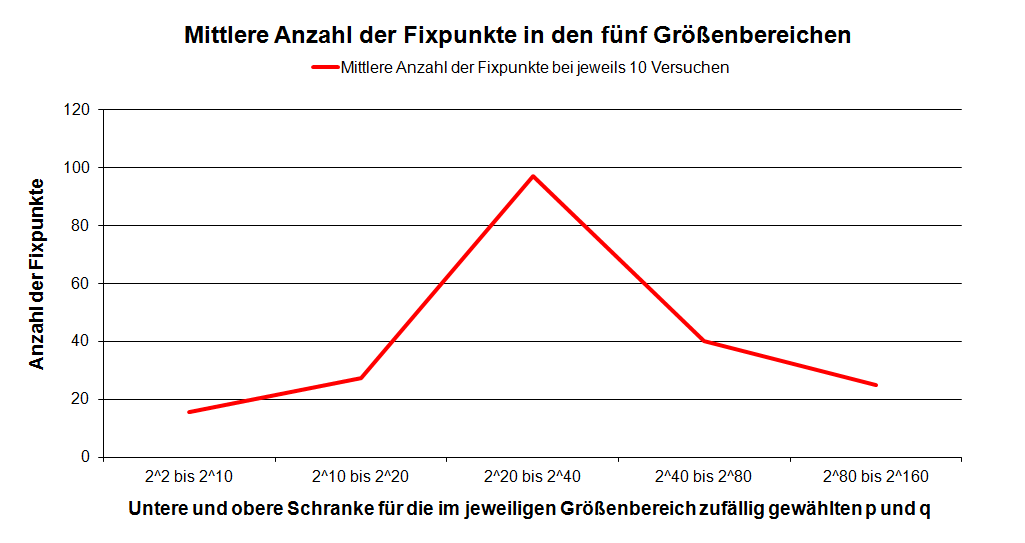
\includegraphics[width=0.92\textwidth]{figures/MAF.png}
  \caption{Eine empirische Abschätzung der Anzahl der Fixpunkte für wachsende Moduli}
  \label{fig:NumberFixpointsGrowingN}
  %\vskip +45pt
\end{figure}

Abbildung \ref{fig:NumberFixpointsGrowingN} zeigt, dass innerhalb der sechs Größenbereiche die durchschnittliche Anzahl der Fixpunkte nicht größer als 40 ist.
% Leider konnten wir die Moduli in noch höheren Bereichen nicht testen, da unser
% SageMath-Programm \ref{nt_sagesample_Calculate_RSA-Fixpoints}  "`Getfixpoints"'
% in Bereichen mit $(p,q) > 2^{320}$ zu langsam ist.\\



\vspace{15pt}
% ----------------------------------------------------
\subsubsection{Beispiel: Bestimmung aller Fixpunkte für einen bestimmten öf\discretionary{-}{}{}fent\-lichen RSA-Schlüssel}

Die Aufgabe besteht darin, alle Fixpunkte für (n, e) = (866959, 17) zu bestimmem.\\

\noindent \textbf{Lösung:}\\
Zuerst faktorisieren wir $n$:  $ 866959 = 811 \cdot 1069$.\\

\noindent Die Anzahl der RSA-Fixpunkte ergibt sich nach Satz \ref{nt-thm-Anzahl-RSA-Fixpunkte}:\\
$ (ggT(  p-1,  e-1)+1) \cdot (ggT(   q-1,  e-1)+1) =
  (ggT(811-1, 17-1)+1) \cdot (ggT(1069-1, 17-1)+1) = (2+1) \cdot (4+1) = 15 $\\

  \noindent Das SageMath-Programm \ref{nt_sagesample_Calculate_RSA-Fixpoints} (Getfixpoints) liefert für $(n,e) = (866959, 17)$ die folgenden 15 Fixpunkte:
%
%\noindent \textbf{3 Fixpunkte modulo p:}\\
%$ ~~~~~0$ (trivialer Fixpunkt manuell hinzugefügt)\\
%$ ~~~~~1$\\
%$ ~~~810$\\
%
%\noindent \textbf{5 Fixpunkte modulo q:}\\
%~~~~~~0 (trivialer Fixpunkt manuell hinzugefügt)\\
%~~~~~~1\\
%~~~~249\\
%~~~~820\\
%~~~1068\\
%
%\noindent \textbf{15 Fixpunkte modulo 866959 bei e= 17:}\\  % TODO_LaTeX: Warum wirkt "~" nicht?
% Deshalb Tabelle statt Liste (spart auch Platz)
%$~~~~~~~~0$\\
%~~~~~~~~1\\
%~~~~23518\\
%~~~~23519\\
%~~~~47037\\
%~~~188964\\
%~~~212482\\
%~~~236000\\
%~~~654477\\
%~~~843440\\
%~~~843441\\
%~~~630959\\
%~~~677995\\
%~~~819922\\
%~~~866958\\
\begin{table}[ht]
\begin{center}
{\tt
\begin{tabular}{llllllll}
     0 &      1 &  23518 &  23519 &  47037\\
188964 & 212482 & 236000 & 654477 & 843440\\
843441 & 630959 & 677995 & 819922 & 866958
\end{tabular} } % tt
\end{center}
\end{table}

\noindent \textbf{Beispiel:}\\
Beispielhaftes Validieren für $ 843441 $:~~
$843441^{17} \mod 866959 = 843441$\\
Also ist $ m = 843441$ ein Fixpunkt für das gegebene $(n,e)$.\\

%%% Leicht modifiziertes SAGE-Programm von Volker Simon (9/2012)
\begin{sagecode}
\begin{Verbatim}%
[fontsize=\footnotesize]
import numpy

print "--- Search for fixpoints in Textbook-RSA given p, q, e ---";
fp=numpy.array([0])
fq=numpy.array([0])

#Edit e,p,q here
###EDIT BEGIN###
e=17;
p=811;
q=1069;
###EDIT END###

n=p*q;
print "Prime p: ",p;
print "Prime q: ",q;
print "Modul n: ",n;
print "Public exponent e: ", e;

r=Integers(p)
gen_f_p = r.multiplicative_generator(); print "\nGenerator of f_p: ",gen_f_p;
s=Integers(q)
gen_f_q = s.multiplicative_generator(); print "Generator of f_q: ",gen_f_q;

gcd_p = gcd(e-1,p-1)
gcd_q = gcd(e-1,q-1)
print "\ngcd(e-1,p-1): ", gcd_p;
print "gcd(e-1,q-1): ", gcd_q;

print "\nNumber of fixpoints: ",(gcd_p+1)*(gcd_q+1);
#Calculating fixpoints modulo F_p
#run i from 0 until gcd(e-1,p-1):
#g^( i*(p-1) / (ggT(e-1,p-1)) ) mod p

print "\nFixpoints modulo p";
print "0 (trivial fixpoint added manually)";
i=0;
for i in range(gcd_p):
                fix_p = power_mod(gen_f_p,Integer(i*(p-1)/gcd_p),p); print fix_p;
                fp = numpy.append(fp,fix_p)

print "\nFixpoints modulo q";
print "0 (trivial fixpoint added manually)";
j=0;
for j in range(gcd_q):
                fix_q = power_mod(gen_f_q,Integer(j*(q-1)/gcd_q),q); print fix_q;
                fq = numpy.append(fq,fix_q);

print "\nFixpoints for the public RSA key (n,e) = (", n, ",", e, ")"
for r in fp:
       for s in fq:
               print crt(Integer(r),Integer(s),Integer(p),Integer(q))

print "\nRemark: You can verify each fixpoint with power_mod(m,e,n).";
\end{Verbatim}
\caption{Bestimmung aller Fixpunkt-Nachrichten für einen gegebenen öffentlichen
         RSA-Schlüssel}
\label{nt_sagesample_Calculate_RSA-Fixpoints}
\end{sagecode}
%#print "        Here done for the last found fixpoint:";
%#m = crt(Integer(r),Integer(s),Integer(p),Integer(q))
%#print "        m = ", m, ",", "power_mod = ", power_mod(m,e,n)
%#if (m != power_mod(m,e,n)):
%#                print "Verification failed !!!";


\vspace{60pt}
\noindent \textbf{Bedeutung der Variablen im SageMath-Code
                  \ref{nt_sagesample_Calculate_RSA-Fixpoints}:}
\begin{Verbatim}%
[fontsize=\footnotesize]
- gen_f_p = r.multiplicative_generator()
  r ist ein Restklassen-Ring modulo p, und multiplicative_generator() gibt
  ein Generator-Element zurück, welches diesen Ring modulo p erzeugt.
- power_mod(gen_f_p,Integer(i*(p-1)/gcd_p),p)
  Die power_mod Funktion potenziert eine Zahl m mit e, und gibt das Ergebnis modulo n aus.
  Bsp.: power_mod(m, e, n) := m^e modulo n
- numpy.append(fp,power_mod(gen_f_p,Integer(i*(p-1)/gcd_p),p))
  Die append Funktion erweitert ein Array (fp) um ein weiteres Element.
- crt(Integer(r),Integer(s),Integer(p),Integer(q))
  CRT steht für Chinese Remainder Theorem. crt(r, s, p, q) löst die Kongruenzen
  x = r mod p und x = s mod q mit Hilfe des Chinesischen Restsatzes.
\end{Verbatim}

%%% xxx111222xxx-end




% ++++++++++++++++++++++++++++++++++++++++++++++++++++++++++++++++++++++++++
\clearpage
\newpage
\hypertarget{NumberTheory_Appendix_F}{}  %\hypertarget{AppendixListAndDef}{}
\section{Anhang: Liste der in diesem Kapitel formulierten Definitionen und Sätze}
\label{l:NumberTheory_Appendix_F}{}  %\label{l:AppendixListAndDef}{}

\begin{center}
\begin{tabular}{|l|l|l|}\hline
 & Kurzbeschreibung~~ & Seite\\ \hline

Definition~\ref{def-zth-prime} & Primzahlen &  \pageref{def-zth-prime}\\
Definition~\ref{def-zth-composite} & Zusammengesetzte Zahlen
                                   & \pageref{def-zth-composite}\\ \hline

Satz~\ref{thm-zth-cnum} & Teiler von zusammengesetzten Zahlen~~~~~~~ & \pageref{thm-zth-cnum}\\
Satz~\ref{thm-zth-mthm} &  Erster Hauptsatz der elementaren Zahlentheorie &  \pageref{thm-zth-mthm}\\  \hline

Definition~\ref{def-zth-divisibility} & Teilbarkeit & \pageref{def-zth-divisibility}\\
Definition~\ref{def-zth-remainder} & Restklasse $r$ modulo $m$ & \pageref{def-zth-remainder}\\
Definition~\ref{def-zth-congruence} & restgleich oder kongruent & \pageref{def-zth-congruence}\\ \hline

Satz~\ref{thm-zth-div} & Kongruenz mittels Differenz & \pageref{thm-zth-div}\\
Satz~\ref{thm-zth-multinv} & Multiplikative Inverse (Existenz) & \pageref{thm-zth-multinv}\\
Satz~\ref{thm-zth-exhperm} & Erschöpfende Permutation & \pageref{thm-zth-exhperm}\\
Satz~\ref{thm-zth-pot} & Gestaffelte Exponentiation mod $m$ & \pageref{thm-zth-pot}\\ \hline

Definition~\ref{def-zth-zn} & $\mathbb{Z}_n$  & \pageref{def-zth-zn}\\
Definition~\ref{def-zth-znmult} &   $\mathbb{Z}_n^*$ & \pageref{def-zth-znmult}\\ \hline

Satz~\ref{thm-zth-znmult} & Multiplikative Inverse in $\mathbb{Z}_n^*$& \pageref{thm-zth-znmult}\\ \hline

Definition~\ref{def-zth-phiofn} & Euler-Funktion $\phi(n)$ & \pageref{def-zth-phiofn}\\
Satz~\ref{thm-zth-phiprime} & $\phi(p)$ &  \pageref{thm-zth-phiprime}\\
Satz~\ref{thm-zth-phipq} & $\phi(p*q)$ &  \pageref{thm-zth-phipq}\\
Satz~\ref{thm-zth-phimultprime} & $\phi(p_1 * \cdots *p_k)$ & \pageref{thm-zth-phimultprime}\\
Satz~\ref{thm-zth-phinum} & $\phi(p_1^{e_1} * \cdots *p_k^{e_k})$ & \pageref{thm-zth-phinum}\\
Satz~\ref{thm-zth-fermat1} & Kleiner Satz von Fermat &  \pageref{thm-zth-fermat1}\\
Satz~\ref{thm-zth-fermateuler} & Satz von Euler-Fermat & \pageref{thm-zth-fermateuler}\\ \hline

Definition~\ref{def-zth-ordn} & Multiplikative Ordnung $ {\rm ord}_{m} (a)$ & \pageref{def-zth-ordn}\\
Definition~\ref{def-zth-primitiveroot} & Primitivwurzel von $m$ &  \pageref{def-zth-primitiveroot}\\
Satz~\ref{thm-zth-ordp} & Ausschöpfung des Wertebereiches & \pageref{thm-zth-ordp}\\ \hline

Satz~\ref{nt-thm-Anzahl-RSA-Fixpunkte} & Anzahl der RSA-Fixpunkte & \pageref{nt-thm-Anzahl-RSA-Fixpunkte}\\ \hline

\end{tabular}
\end{center}
\vskip +6 pt





%------------------------------------------------------------------------------
\printbibliography[%
	heading=subbibintoc,
	title={Literatur zu Kapitel \thechapter},
	segment=\therefsegment,
]


\noindent Alle Links wurden am 12.07.2016 überprüft.



% ++++++++++++++++++++++++++++++++++++++++++++++++++++++++++++++++++++++++++
\newpage
\section*{Web-Links}\addcontentsline{toc}{section}{Web-Links}

\begin{enumerate}
   \item \hypertarget{knott}{} \index{Knott, Ron}
          Fibonacci-Seite\index{Fibonacci} von Ron Knott\\
          Hier dreht sich alles um Fibonacci-Zahlen.\\
          \url{http://www.maths.surrey.ac.uk/hosted-sites/R.Knott/Fibonacci/fib.html}

   \item CrypTool\index{CrypTool}\\
          E-Learning-Freeware zur Veranschaulichung von Kryptographie
          und Kryptoanalyse\\
          \url{http://www.cryptool.de},\\
          \url{http://www.cryptool.org}

   \item Mathematica \index{Mathematica}\\
          Kommerzielles Mathematik-Paket\\
          \url{http://www.wolfram.com}

   \item  LiDIA \index{LiDIA 2000}\\
          Umfangreiche Bibliothek mit zahlentheoretischen Funktionen und der
          Interpretersprache LC. LiDIA wird seit 2000 nicht weiter entwickelt.\\
          \url{http://cs.nyu.edu/exact/core/download/core_v1.3/core_v1.3/lidia/}

   \item BC \index{BC}\\
         Interpreter mit zahlentheoretischen Funktionen. Wird leider seit 2006
	 nicht weiter entwickelt und funktioniert unter neueren Windows-Versionen
	 auch nicht mehr korrekt.\\
	 Von Keith Matthews gibt es für Unix aber regelmäßig keine Updates.\\
         \url{http://www.gnu.org/software/bc/bc.html}\\
         \url{http://www.numbertheory.org/gnubc/gnubc.html}

   \item Pari-GP \index{Pari-GP}\\
         Schneller und freier Interpreter mit zahlentheoretischen Funktionen.
	 Auch im Browser. Gepflegt von Karim Belabas.\\
         \url{http://pari.math.u-bordeaux.fr/}\\%% http://pari.math.u-bordeaux1.fr/
         \url{http://pari.math.u-bordeaux.fr/gp.html}\\
         \url{http://en.wikipedia.org/wiki/PARI/GP}

   \item\sloppy SageMath\index{SageMath}\\
         Ausgezeichnetes Open-Source Computer-Algebra-System, basierend auf Python\index{Python}
	 als Skript-Sprache. Damit sind die Code-Beispiele in diesem Kapitel erstellt.
	 Vergleiche hierzu die Einführung in Kapitel~\ref{s:appendix-using-sage}.\\
         \url{http://www.sagemath.org/}\\
         \url{https://de.wikipedia.org/wiki/Sage_(Software)}

   \item Münchenbach\index{Munchenbach@Münchenbach, Carsten}\\
         Erst nach Vollendung der ersten Versionen dieses Artikels wurde mir die Web-Seite von
	 Herrn Münchenbach (1999) bekannt, die interaktiv und didaktisch sehr
         ausgereift die grundlegenden Denkweisen der Mathematik anhand
         der elementaren Zahlentheorie nahebringt. Sie entstand für
         ein Unterrichtsprojekt der 11. Klasse des Technischen Gymnasiums
         und nutzt MuPAD (leider nur in Deutsch verfügbar).\\
         \url{http://www.hydrargyrum.de/kryptographie}

   \item Wagner\\
	 Seite des Beauftragten für die Lehrplanentwicklung des Fachs
         Informatik an der gymnasialen Oberstufe des Landes Saarland aus 2012.
         Hier befindet sich eine Sammlung von Texten und Programmen
         (in Java), die aus didaktischen Überlegungen entstand (alles
         nur in Deutsch verfügbar).\\
         \url{http://www.saar.de/~awa/kryptologie.html}\\
         \url{http://www.saar.de/~awa/menu_kryptologie.html}

   \item BSI\index{BSI}\\
         Bundesamt für Sicherheit in der Informationstechnik\\
         \url{http://www.bsi.bund.de}


   \item Faktorisierungsrekorde und Challenges
	 \index{Faktorisierung!Faktorisierungsrekorde}
	 \index{Faktorisierung!Faktorisierungs-Challenges}\\
         \url{https://web.archive.org/web/20170704003418/http://www.crypto-world.com:80/},~~ letztes Update 2013\\
         \url{https://web.archive.org/web/20170518021747/http://www.crypto-world.com:80/FactorWorld.html},~~ Webseite von Scott Contini\\
         \url{http://www.loria.fr/~zimmerma/records/factor.html}\\
	 \url{http://www.emc.com/emc-plus/rsa-labs/historical/the-rsa-factoring-challenge.htm}

         \url{https://www.uni-bonn.de/Pressemitteilungen/004-2010},~~ zu RSA-768\\
         \url{https://members.loria.fr/PZimmermann/records/gnfs158},~~ zu C158\\
         \url{http://www.loria.fr/~zimmerma/records/rsa160}

         % Toter Link: \url{http://www.tutorgig.com/ed/RSA\_number}
	 % Toter Link: \url{http://www.ercim.org/publication/Ercim\_News/enw49/franke.html}\\ %2002-01
         % Toter Link: \url{http://www.rsa.com/rsalabs/node.asp?id=2092}
	

   \item Das Cunningham-Projekt\index{Cunningham-Projekt}\\
         \url{http://www.cerias.purdue.edu/homes/ssw/cun/},~~ letzte Änderung 11.05.2016

   \item Daniel J. Bernsteins Webseiten\\
	 \url{http://cr.yp.to}

   \item Post-Quantum-Kryptographie\\
	 \url{http://pqcrypto.org/}

\end{enumerate}

\noindent Alle Links wurden am 06.08.2018 überprüft.



% ++++++++++++++++++++++++++++++++++++++++++++++++++++++++++++++++++++++++++
\vskip +20 pt
\section*{Dank} \addcontentsline{toc}{section}{Dank}
Ich möchte hier die Gelegenheit nutzen, den folgenden Personen ganz
herzlich zu danken:
\begin{itemize}

  \item {Hr. Henrik Koy für das anregende und sehr konstruktive
         Korrekturlesen und die vielen Verbesserungen der ersten
	 Version dieses Artikels, und für die Hilfen bei TeX, ohne die
	 dieser Artikel nie in dieser Form erschienen wäre.}
%	 RSA-Krypto"-system   (TRENNUNG erzwingen)

  \item {Jörg Cornelius Schneider für die engagierte Unterstützung bei TeX und
         die mannigfaltigen Hilfen bei allen Arten von Programmier- und
	 Design-Problemen.}

  \item {Dr. Georg Illies für den Hinweis auf Pari-GP\index{Pari-GP}.}

  \item {Lars Fischer für seine Hilfe bei schnellem Pari-GP\index{Pari-GP}-Code
         für Primitivwurzeln.}

  \item {Minh Van Nguyen aus Australien für seine immer schnelle, kompetente und
         ausführliche Hilfe bei den ersten SageMath\index{SageMath}-Code-Beispielen
	 in diesem Kapitel. Schade, dass er nicht mehr erreichbar ist ...}

\end{itemize}

\end{refsegment}

% Local Variables:
% TeX-master: "../script-de.tex"
% End:
